\documentclass[10pt]{report}
\usepackage{lmodern}
\usepackage{graphicx}
\usepackage{varwidth}
\usepackage{enumitem}
\usepackage{amsmath}
\usepackage{amssymb}
\usepackage{mathtools}
\usepackage{pifont}
\usepackage{arydshln}
\usepackage{tikz}
\usepackage{lscape}
\usepackage{bm}
\usepackage{nicefrac}
\usepackage{physics}
\usepackage{fontsize}
\usepackage[landscape]{geometry}
\geometry{a4paper, total={296mm,210mm}, left=-5mm, top=0mm}
\renewcommand{\labelenumi}{\bfseries(\alph{enumi})\phantom{x}}
\newcommand\omicron{o}
\hfuzz=50pt
\setlist[enumerate]{leftmargin=0pt,itemindent=34pt}
\pagenumbering{gobble}
\setlength{\tabcolsep}{0pt}
\begin{document}
\thispagestyle{empty}
\begin{tabular}{c:c}
\begin{minipage}[c][104.5mm][t]{0.5\linewidth}
\begin{center}
\vspace{7mm}
{\huge Kvadratická rovnice, skupina \textit{Alpha $\alpha$} -\romannumeral1}\\[5mm]
\textit{Jméno:}\phantom{xxxxxxxxxxxxxxxxxxxxxxxxxxxxxxxxxxxxxxxxxxxxxxxxxxxxxxxxxxxxxxxxx}\\[5mm]
\begin{minipage}{0.95\linewidth}
\begin{center}
V \textbf{(a)} a \textbf{(b)} zjisti počet řešení. V \textbf{(c)} x-ovú polohu vrcholu, a v \textbf{(d)} y-ovú polohu vrcholu.\\V \textbf{(e)} a \textbf{(f)} zjisti součet řešení. Pokud ti vyjde stejný výsledek jako je za otazníky, tak\\napravo obarvi příslušející kroužek načerno. \textbf{Spolu odevzdejte výsledné slovo}.
\end{center}
\end{minipage}
\\[1mm]
\begin{minipage}{0.79\linewidth}
\begin{center}
\begin{varwidth}{\linewidth}
\begin{enumerate}
\Large
\item $4x^2-6x+6=0$\quad \dotfill\; ???\;\dotfill \quad 0
\item $x^2-2x-3=0$\quad \dotfill\; ???\;\dotfill \quad 0
\item $f(x)=-5x^2+4x+3$\quad \dotfill\; ???\;\dotfill \quad $\nicefrac{-2}{5}$
\item $f(x)=-4x^2+3x-4$\quad \dotfill\; ???\;\dotfill \quad $\nicefrac{-55}{16}$
\item $9x^2+27x+18=0$\quad \dotfill\; ???\;\dotfill \quad -3
\item $4x^2-9x+2=0$\quad \dotfill\; ???\;\dotfill \quad $\nicefrac{-7}{4}$
\end{enumerate}
\end{varwidth}
\end{center}
\end{minipage}
\begin{minipage}{0.20\linewidth}
\begin{center}
{\Huge\bfseries 1.} \\[2mm]
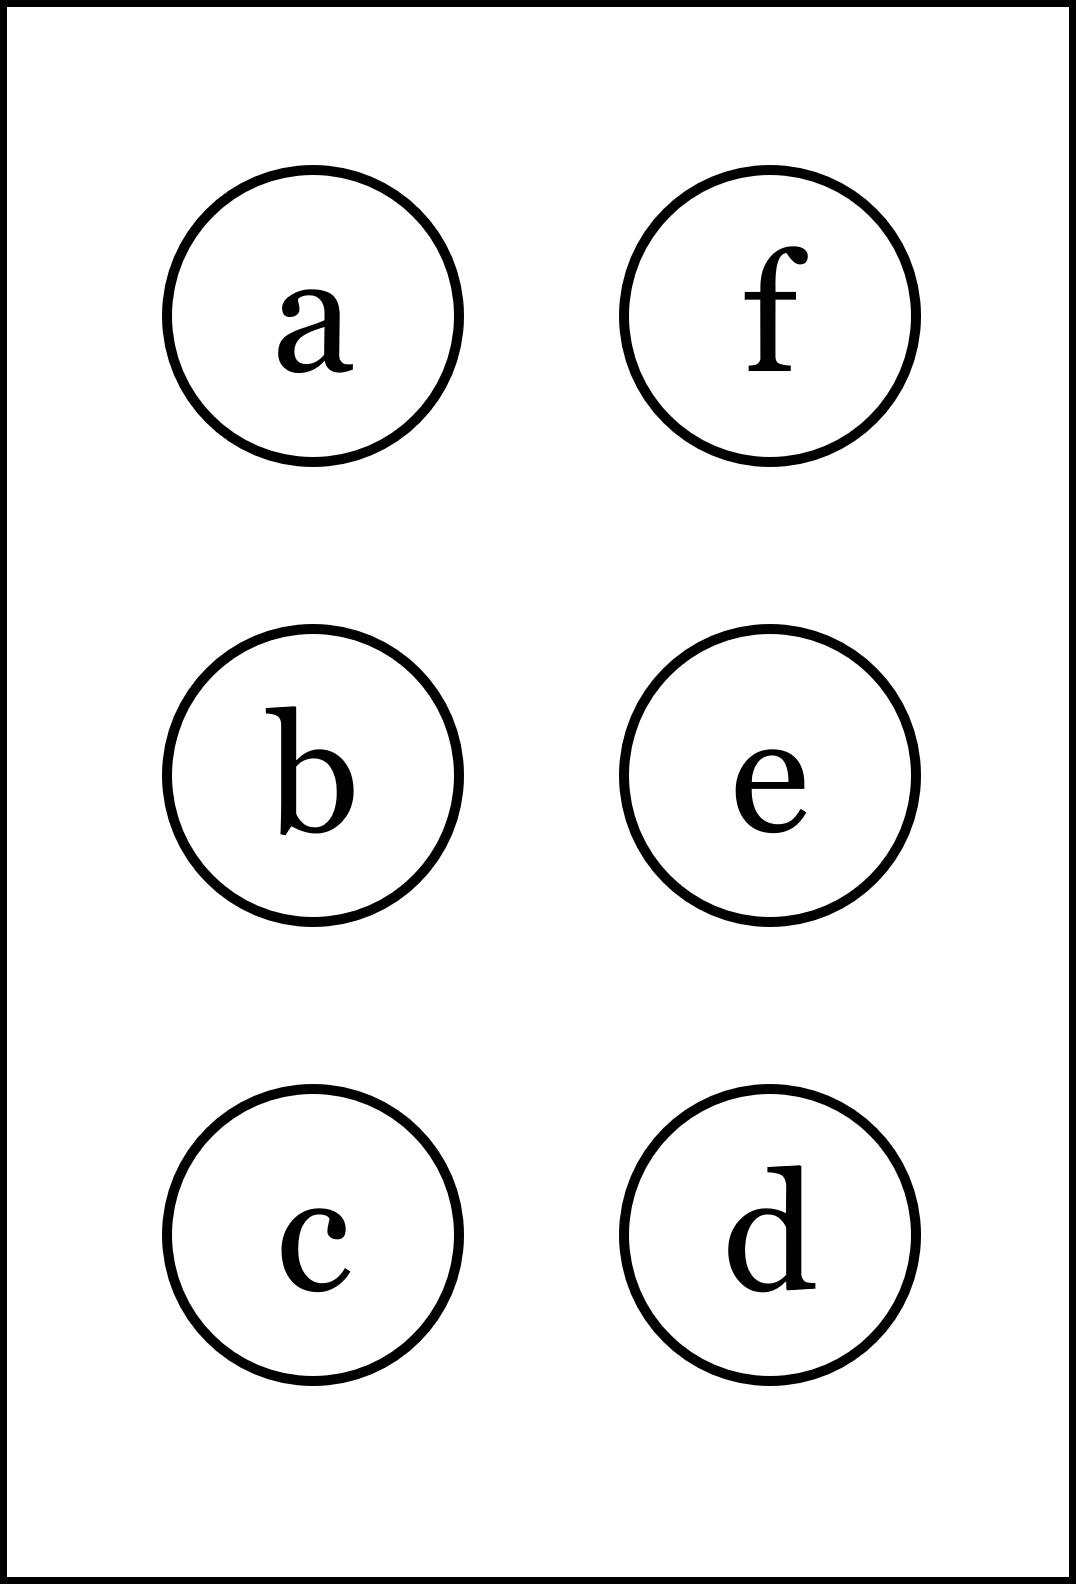
\includegraphics[height=40mm]{../images/braille.png}
{\small Písmeno Braillovej abecedy}
\end{center}
\end{minipage}
\end{center}
\end{minipage}
&
\begin{minipage}[c][104.5mm][t]{0.5\linewidth}
\begin{center}
\vspace{7mm}
{\huge Kvadratická rovnice, skupina \textit{Alpha $\alpha$} -\romannumeral2}\\[5mm]
\textit{Jméno:}\phantom{xxxxxxxxxxxxxxxxxxxxxxxxxxxxxxxxxxxxxxxxxxxxxxxxxxxxxxxxxxxxxxxxx}\\[5mm]
\begin{minipage}{0.95\linewidth}
\begin{center}
V \textbf{(a)} a \textbf{(b)} zjisti počet řešení. V \textbf{(c)} x-ovú polohu vrcholu, a v \textbf{(d)} y-ovú polohu vrcholu.\\V \textbf{(e)} a \textbf{(f)} zjisti součet řešení. Pokud ti vyjde stejný výsledek jako je za otazníky, tak\\napravo obarvi příslušející kroužek načerno. \textbf{Spolu odevzdejte výsledné slovo}.
\end{center}
\end{minipage}
\\[1mm]
\begin{minipage}{0.79\linewidth}
\begin{center}
\begin{varwidth}{\linewidth}
\begin{enumerate}
\Large
\item $8x^2+3x+1=0$\quad \dotfill\; ???\;\dotfill \quad 0
\item $-8x^2-5x+2=0$\quad \dotfill\; ???\;\dotfill \quad 0
\item $f(x)=3x^2-3x-5$\quad \dotfill\; ???\;\dotfill \quad $\nicefrac{1}{2}$
\item $f(x)=-3x^2-6x+1$\quad \dotfill\; ???\;\dotfill \quad $\nicefrac{7}{2}$
\item $-x^2+3x+18=0$\quad \dotfill\; ???\;\dotfill \quad 3
\item $40x^2-13x+1=0$\quad \dotfill\; ???\;\dotfill \quad $\nicefrac{13}{40}$
\end{enumerate}
\end{varwidth}
\end{center}
\end{minipage}
\begin{minipage}{0.20\linewidth}
\begin{center}
{\Huge\bfseries 2.} \\[2mm]
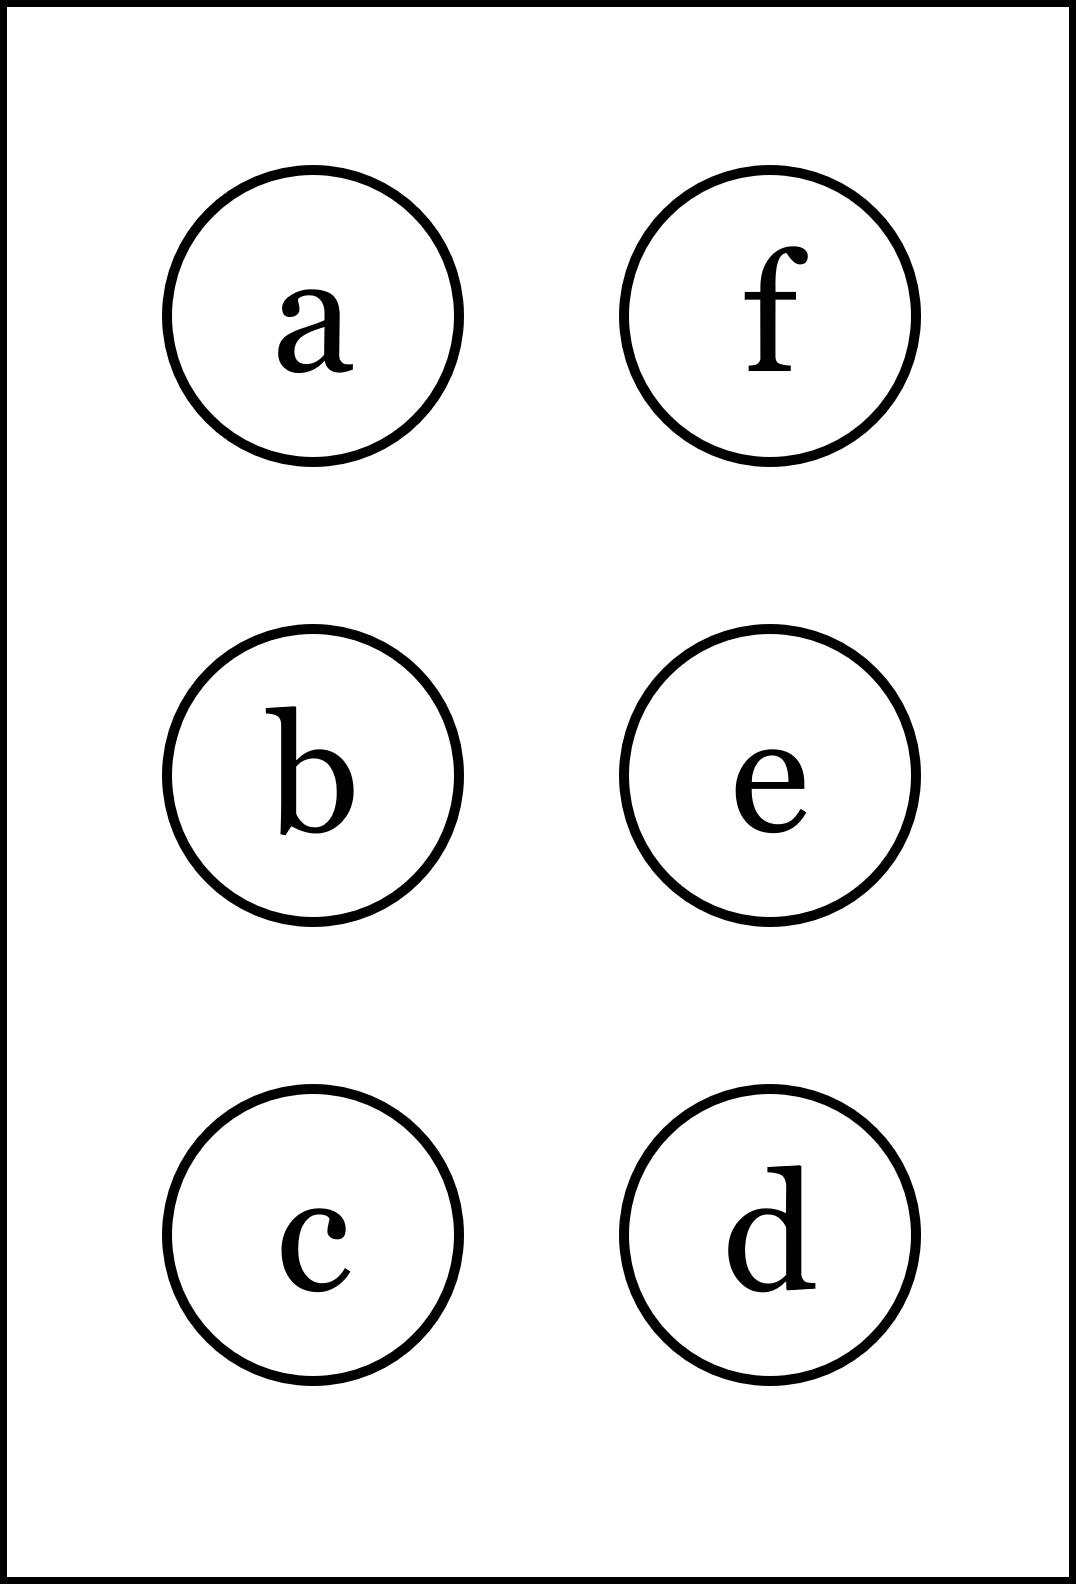
\includegraphics[height=40mm]{../images/braille.png}
{\small Písmeno Braillovej abecedy}
\end{center}
\end{minipage}
\end{center}
\end{minipage}
\\ \hdashline
\begin{minipage}[c][104.5mm][t]{0.5\linewidth}
\begin{center}
\vspace{7mm}
{\huge Kvadratická rovnice, skupina \textit{Alpha $\alpha$} -\romannumeral3}\\[5mm]
\textit{Jméno:}\phantom{xxxxxxxxxxxxxxxxxxxxxxxxxxxxxxxxxxxxxxxxxxxxxxxxxxxxxxxxxxxxxxxxx}\\[5mm]
\begin{minipage}{0.95\linewidth}
\begin{center}
V \textbf{(a)} a \textbf{(b)} zjisti počet řešení. V \textbf{(c)} x-ovú polohu vrcholu, a v \textbf{(d)} y-ovú polohu vrcholu.\\V \textbf{(e)} a \textbf{(f)} zjisti součet řešení. Pokud ti vyjde stejný výsledek jako je za otazníky, tak\\napravo obarvi příslušející kroužek načerno. \textbf{Spolu odevzdejte výsledné slovo}.
\end{center}
\end{minipage}
\\[1mm]
\begin{minipage}{0.79\linewidth}
\begin{center}
\begin{varwidth}{\linewidth}
\begin{enumerate}
\Large
\item $x^2-2x-3=0$\quad \dotfill\; ???\;\dotfill \quad 2
\item $6x^2-3x-7=0$\quad \dotfill\; ???\;\dotfill \quad 1
\item $f(x)=6x^2+x-2$\quad \dotfill\; ???\;\dotfill \quad $\nicefrac{1}{12}$
\item $f(x)=-4x^2+x+6$\quad \dotfill\; ???\;\dotfill \quad $\nicefrac{49}{16}$
\item $-3x^2-12x+15=0$\quad \dotfill\; ???\;\dotfill \quad -4
\item $-10x^2+11x-3=0$\quad \dotfill\; ???\;\dotfill \quad $\nicefrac{-1}{10}$
\end{enumerate}
\end{varwidth}
\end{center}
\end{minipage}
\begin{minipage}{0.20\linewidth}
\begin{center}
{\Huge\bfseries 3.} \\[2mm]
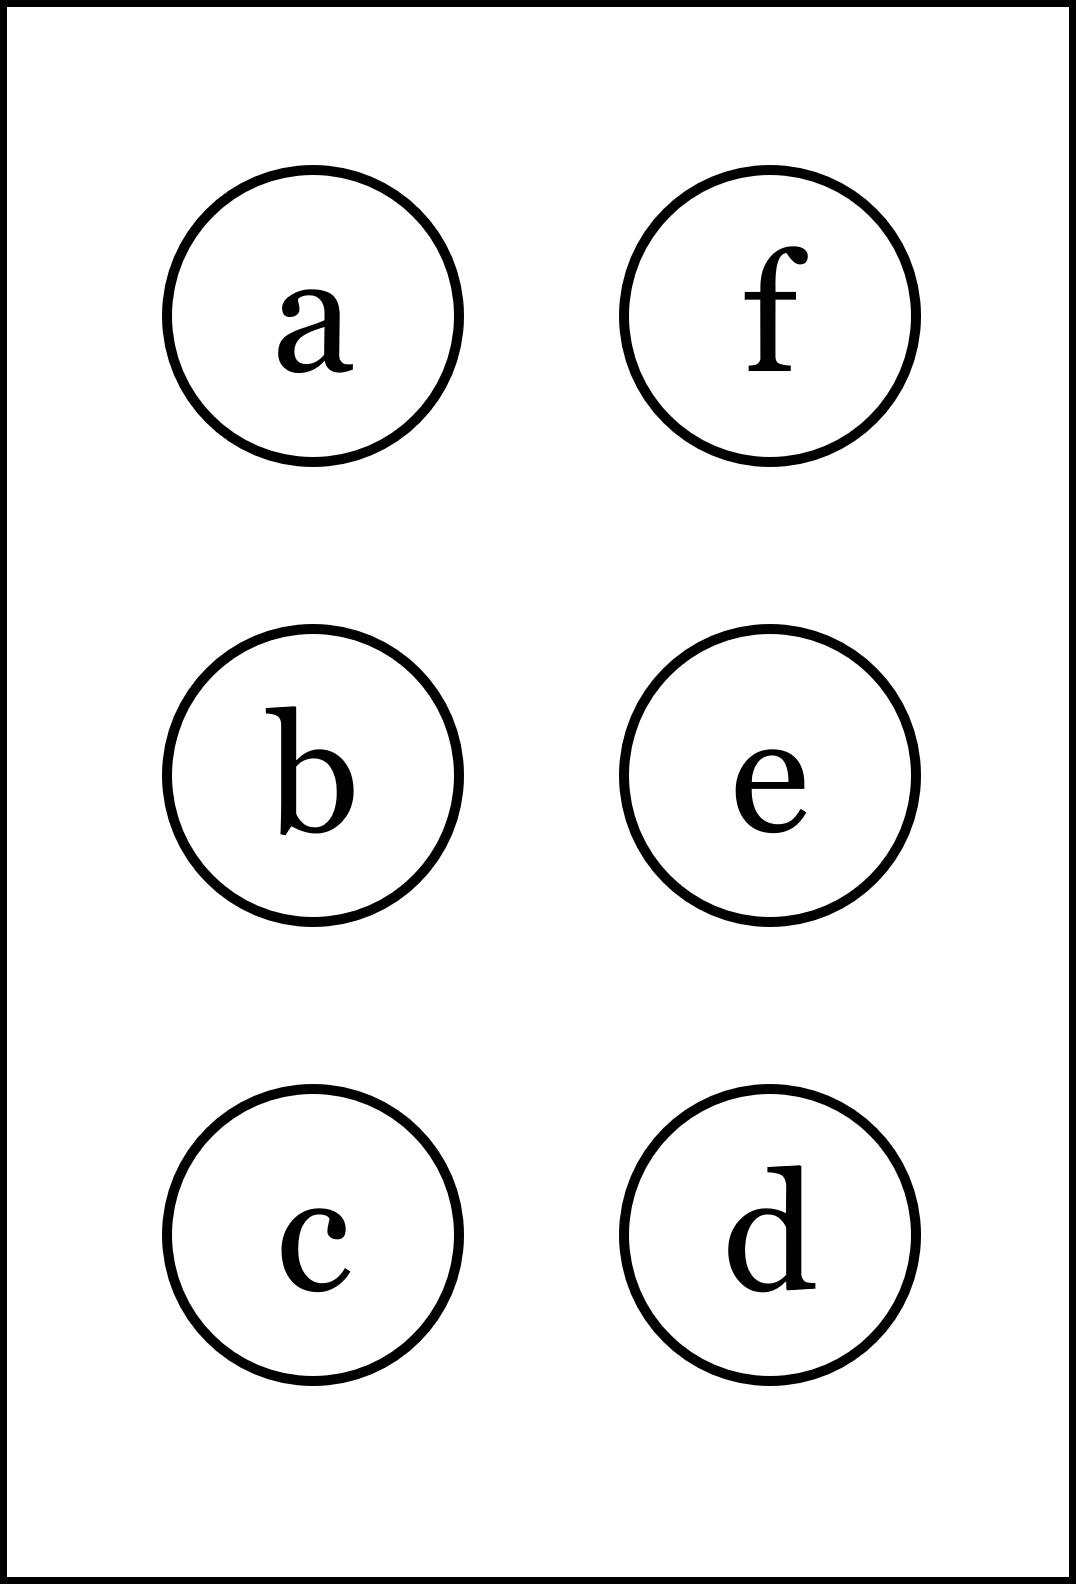
\includegraphics[height=40mm]{../images/braille.png}
{\small Písmeno Braillovej abecedy}
\end{center}
\end{minipage}
\end{center}
\end{minipage}
&
\begin{minipage}[c][104.5mm][t]{0.5\linewidth}
\begin{center}
\vspace{7mm}
{\huge Kvadratická rovnice, skupina \textit{Alpha $\alpha$} -\romannumeral4}\\[5mm]
\textit{Jméno:}\phantom{xxxxxxxxxxxxxxxxxxxxxxxxxxxxxxxxxxxxxxxxxxxxxxxxxxxxxxxxxxxxxxxxx}\\[5mm]
\begin{minipage}{0.95\linewidth}
\begin{center}
V \textbf{(a)} a \textbf{(b)} zjisti počet řešení. V \textbf{(c)} x-ovú polohu vrcholu, a v \textbf{(d)} y-ovú polohu vrcholu.\\V \textbf{(e)} a \textbf{(f)} zjisti součet řešení. Pokud ti vyjde stejný výsledek jako je za otazníky, tak\\napravo obarvi příslušející kroužek načerno. \textbf{Spolu odevzdejte výsledné slovo}.
\end{center}
\end{minipage}
\\[1mm]
\begin{minipage}{0.79\linewidth}
\begin{center}
\begin{varwidth}{\linewidth}
\begin{enumerate}
\Large
\item $-x^2-5x+2=0$\quad \dotfill\; ???\;\dotfill \quad 2
\item $5x^2-9x+4=0$\quad \dotfill\; ???\;\dotfill \quad 0
\item $f(x)=-4x^2-2x+2$\quad \dotfill\; ???\;\dotfill \quad $\nicefrac{-1}{4}$
\item $f(x)=-6x^2+9x-3$\quad \dotfill\; ???\;\dotfill \quad $\nicefrac{15}{8}$
\item $-x^2+10x-16=0$\quad \dotfill\; ???\;\dotfill \quad 8
\item $-24x^2+14x-2=0$\quad \dotfill\; ???\;\dotfill \quad $\nicefrac{-1}{12}$
\end{enumerate}
\end{varwidth}
\end{center}
\end{minipage}
\begin{minipage}{0.20\linewidth}
\begin{center}
{\Huge\bfseries 4.} \\[2mm]
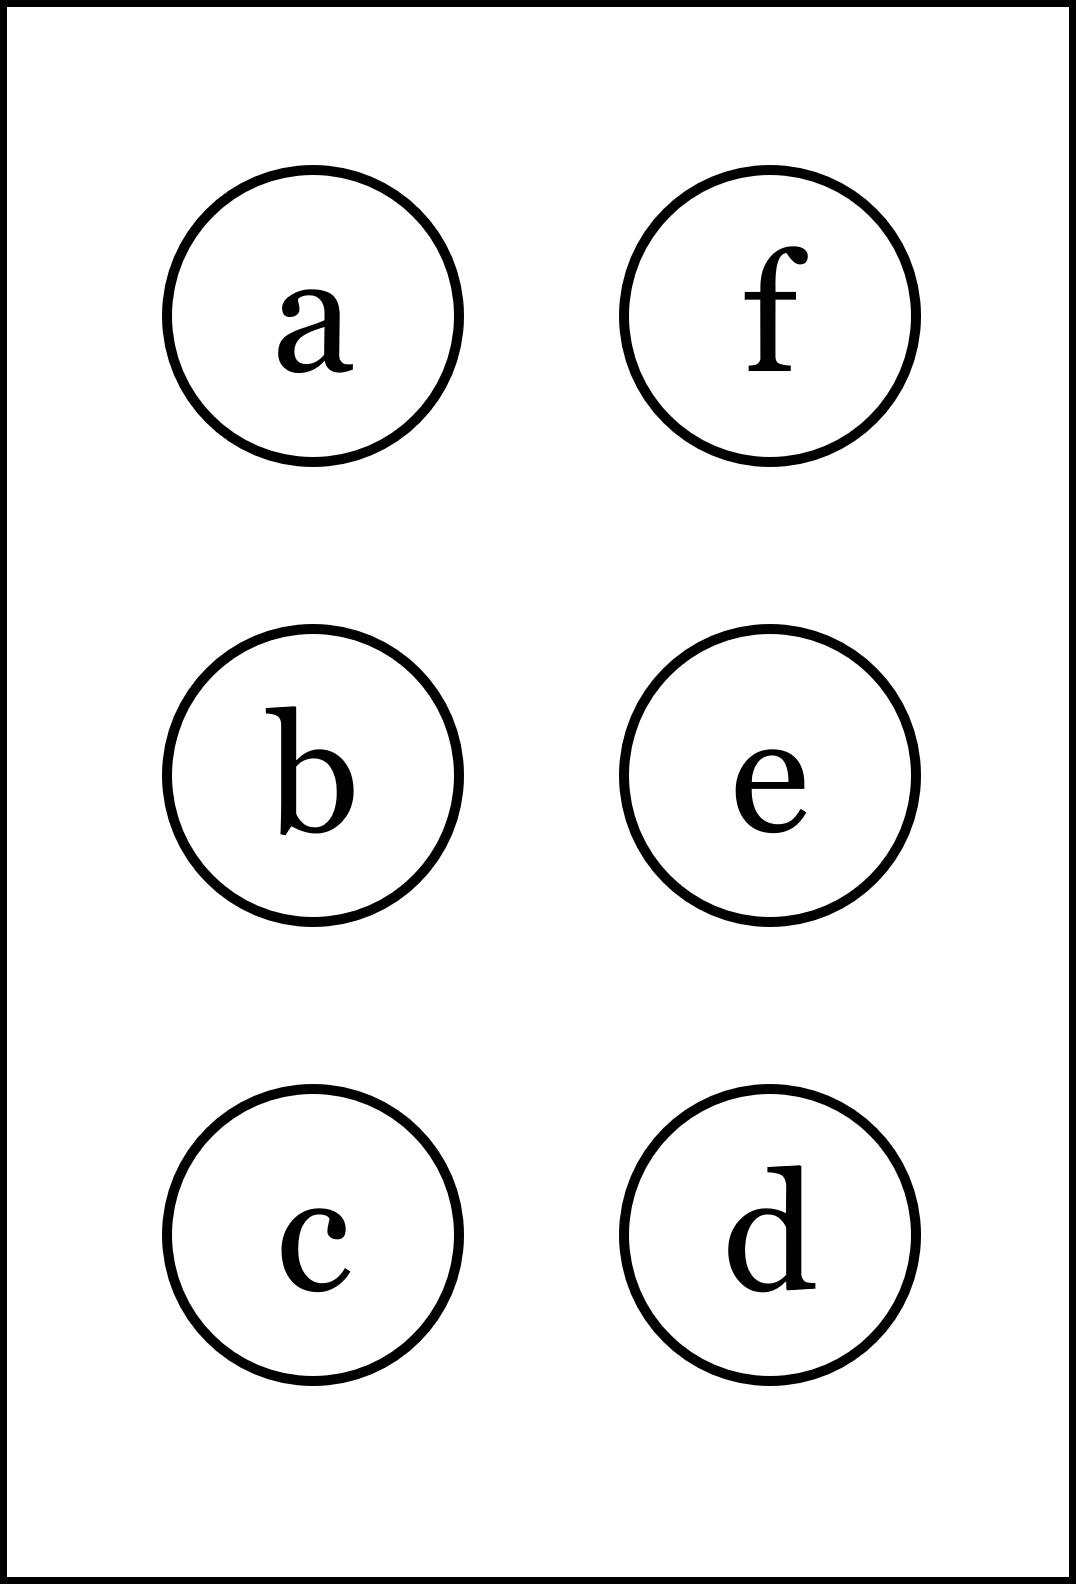
\includegraphics[height=40mm]{../images/braille.png}
{\small Písmeno Braillovej abecedy}
\end{center}
\end{minipage}
\end{center}
\end{minipage}
%
\end{tabular}
\newpage
\thispagestyle{empty}
\begin{tabular}{c:c}
\begin{minipage}[c][104.5mm][t]{0.5\linewidth}
\begin{center}
\vspace{7mm}
{\huge Kvadratická rovnice, skupina \textit{Beta $\beta$} -\romannumeral1}\\[5mm]
\textit{Jméno:}\phantom{xxxxxxxxxxxxxxxxxxxxxxxxxxxxxxxxxxxxxxxxxxxxxxxxxxxxxxxxxxxxxxxxx}\\[5mm]
\begin{minipage}{0.95\linewidth}
\begin{center}
V \textbf{(a)} a \textbf{(b)} zjisti počet řešení. V \textbf{(c)} x-ovú polohu vrcholu, a v \textbf{(d)} y-ovú polohu vrcholu.\\V \textbf{(e)} a \textbf{(f)} zjisti součet řešení. Pokud ti vyjde stejný výsledek jako je za otazníky, tak\\napravo obarvi příslušející kroužek načerno. \textbf{Spolu odevzdejte výsledné slovo}.
\end{center}
\end{minipage}
\\[1mm]
\begin{minipage}{0.79\linewidth}
\begin{center}
\begin{varwidth}{\linewidth}
\begin{enumerate}
\Large
\item $3x^2-6x-5=0$\quad \dotfill\; ???\;\dotfill \quad 2
\item $-4x^2+x+2=0$\quad \dotfill\; ???\;\dotfill \quad 2
\item $f(x)=-3x^2+3x+1$\quad \dotfill\; ???\;\dotfill \quad $\nicefrac{-1}{2}$
\item $f(x)=-6x^2+2x-6$\quad \dotfill\; ???\;\dotfill \quad $\nicefrac{-17}{6}$
\item $-x^2-9x-20=0$\quad \dotfill\; ???\;\dotfill \quad -9
\item $-4x^2-2x+2=0$\quad \dotfill\; ???\;\dotfill \quad $\nicefrac{3}{2}$
\end{enumerate}
\end{varwidth}
\end{center}
\end{minipage}
\begin{minipage}{0.20\linewidth}
\begin{center}
{\Huge\bfseries 1.} \\[2mm]
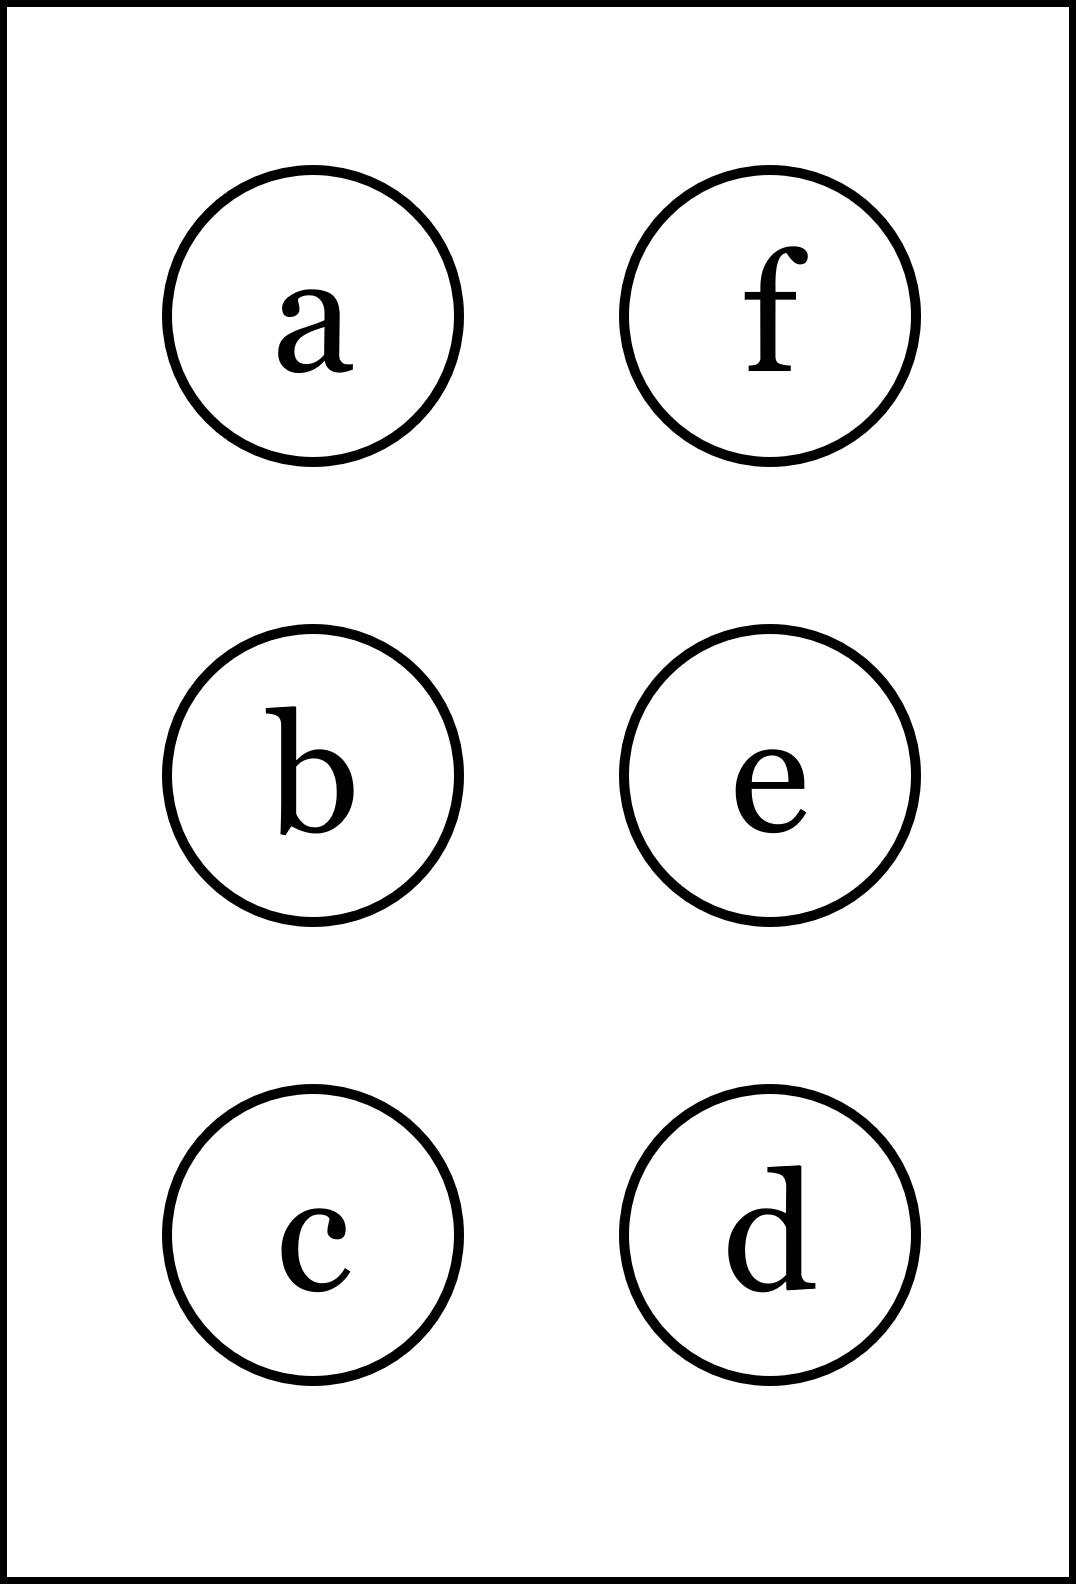
\includegraphics[height=40mm]{../images/braille.png}
{\small Písmeno Braillovej abecedy}
\end{center}
\end{minipage}
\end{center}
\end{minipage}
&
\begin{minipage}[c][104.5mm][t]{0.5\linewidth}
\begin{center}
\vspace{7mm}
{\huge Kvadratická rovnice, skupina \textit{Beta $\beta$} -\romannumeral2}\\[5mm]
\textit{Jméno:}\phantom{xxxxxxxxxxxxxxxxxxxxxxxxxxxxxxxxxxxxxxxxxxxxxxxxxxxxxxxxxxxxxxxxx}\\[5mm]
\begin{minipage}{0.95\linewidth}
\begin{center}
V \textbf{(a)} a \textbf{(b)} zjisti počet řešení. V \textbf{(c)} x-ovú polohu vrcholu, a v \textbf{(d)} y-ovú polohu vrcholu.\\V \textbf{(e)} a \textbf{(f)} zjisti součet řešení. Pokud ti vyjde stejný výsledek jako je za otazníky, tak\\napravo obarvi příslušející kroužek načerno. \textbf{Spolu odevzdejte výsledné slovo}.
\end{center}
\end{minipage}
\\[1mm]
\begin{minipage}{0.79\linewidth}
\begin{center}
\begin{varwidth}{\linewidth}
\begin{enumerate}
\Large
\item $5x^2+5x-1=0$\quad \dotfill\; ???\;\dotfill \quad 2
\item $-7x^2-5x+7=0$\quad \dotfill\; ???\;\dotfill \quad 1
\item $f(x)=3x^2-6x+4$\quad \dotfill\; ???\;\dotfill \quad $-1$
\item $f(x)=2x^2-7x-8$\quad \dotfill\; ???\;\dotfill \quad $\nicefrac{-81}{8}$
\item $-x^2-x+6=0$\quad \dotfill\; ???\;\dotfill \quad -4
\item $3x^2-6x-9=0$\quad \dotfill\; ???\;\dotfill \quad $-4$
\end{enumerate}
\end{varwidth}
\end{center}
\end{minipage}
\begin{minipage}{0.20\linewidth}
\begin{center}
{\Huge\bfseries 2.} \\[2mm]
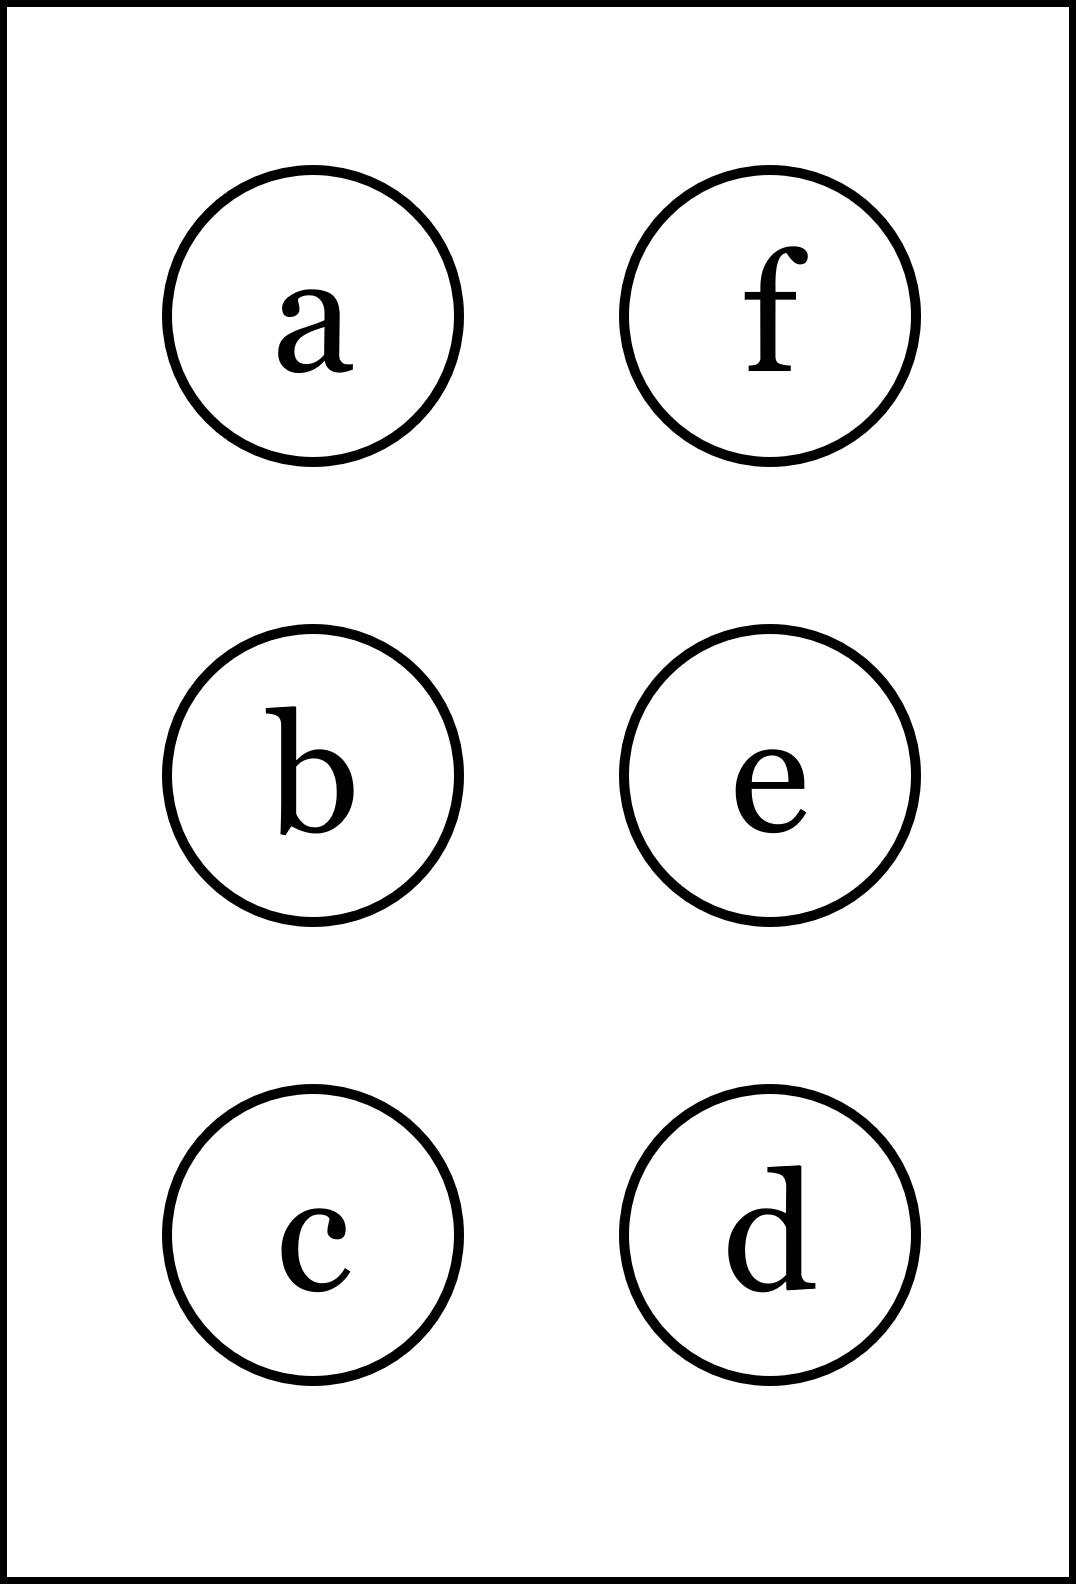
\includegraphics[height=40mm]{../images/braille.png}
{\small Písmeno Braillovej abecedy}
\end{center}
\end{minipage}
\end{center}
\end{minipage}
\\ \hdashline
\begin{minipage}[c][104.5mm][t]{0.5\linewidth}
\begin{center}
\vspace{7mm}
{\huge Kvadratická rovnice, skupina \textit{Beta $\beta$} -\romannumeral3}\\[5mm]
\textit{Jméno:}\phantom{xxxxxxxxxxxxxxxxxxxxxxxxxxxxxxxxxxxxxxxxxxxxxxxxxxxxxxxxxxxxxxxxx}\\[5mm]
\begin{minipage}{0.95\linewidth}
\begin{center}
V \textbf{(a)} a \textbf{(b)} zjisti počet řešení. V \textbf{(c)} x-ovú polohu vrcholu, a v \textbf{(d)} y-ovú polohu vrcholu.\\V \textbf{(e)} a \textbf{(f)} zjisti součet řešení. Pokud ti vyjde stejný výsledek jako je za otazníky, tak\\napravo obarvi příslušející kroužek načerno. \textbf{Spolu odevzdejte výsledné slovo}.
\end{center}
\end{minipage}
\\[1mm]
\begin{minipage}{0.79\linewidth}
\begin{center}
\begin{varwidth}{\linewidth}
\begin{enumerate}
\Large
\item $3x^2-2x-6=0$\quad \dotfill\; ???\;\dotfill \quad 2
\item $5x^2+5x+8=0$\quad \dotfill\; ???\;\dotfill \quad 1
\item $f(x)=8x^2-2x+6$\quad \dotfill\; ???\;\dotfill \quad $\nicefrac{1}{8}$
\item $f(x)=7x^2-x+7$\quad \dotfill\; ???\;\dotfill \quad $\nicefrac{97}{28}$
\item $-2x^2+6x+8=0$\quad \dotfill\; ???\;\dotfill \quad 3
\item $-6x^2-5x+4=0$\quad \dotfill\; ???\;\dotfill \quad $\nicefrac{-5}{6}$
\end{enumerate}
\end{varwidth}
\end{center}
\end{minipage}
\begin{minipage}{0.20\linewidth}
\begin{center}
{\Huge\bfseries 3.} \\[2mm]
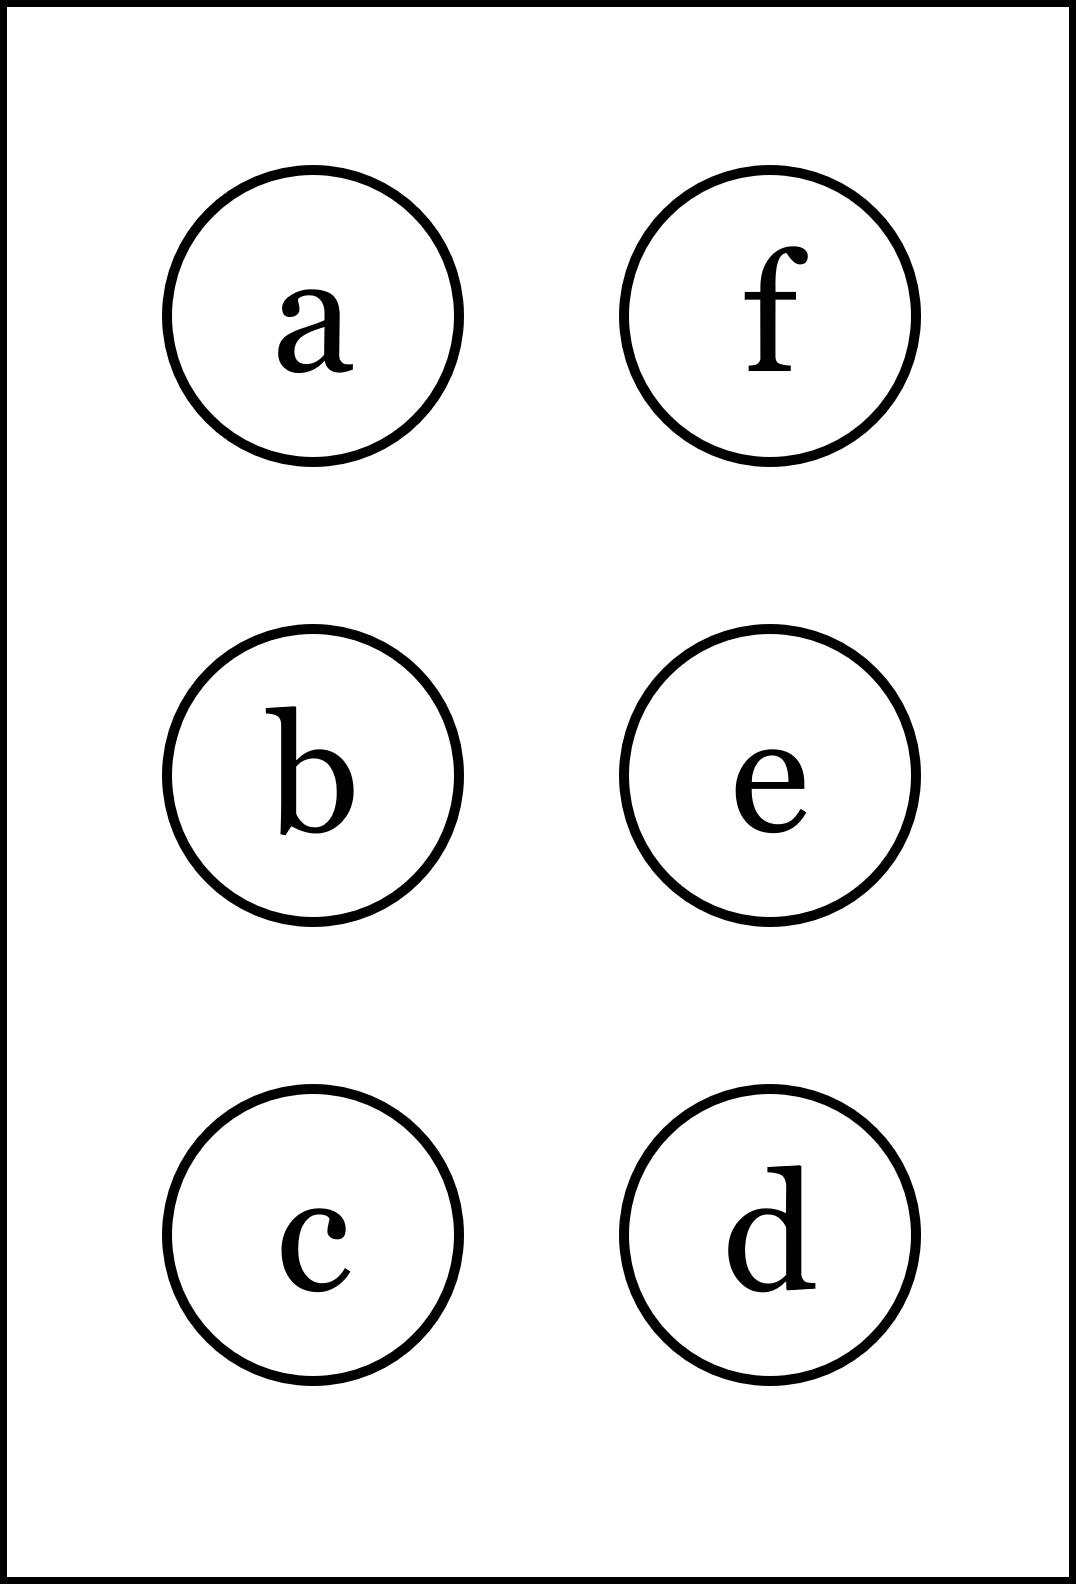
\includegraphics[height=40mm]{../images/braille.png}
{\small Písmeno Braillovej abecedy}
\end{center}
\end{minipage}
\end{center}
\end{minipage}
&
\begin{minipage}[c][104.5mm][t]{0.5\linewidth}
\begin{center}
\vspace{7mm}
{\huge Kvadratická rovnice, skupina \textit{Beta $\beta$} -\romannumeral4}\\[5mm]
\textit{Jméno:}\phantom{xxxxxxxxxxxxxxxxxxxxxxxxxxxxxxxxxxxxxxxxxxxxxxxxxxxxxxxxxxxxxxxxx}\\[5mm]
\begin{minipage}{0.95\linewidth}
\begin{center}
V \textbf{(a)} a \textbf{(b)} zjisti počet řešení. V \textbf{(c)} x-ovú polohu vrcholu, a v \textbf{(d)} y-ovú polohu vrcholu.\\V \textbf{(e)} a \textbf{(f)} zjisti součet řešení. Pokud ti vyjde stejný výsledek jako je za otazníky, tak\\napravo obarvi příslušející kroužek načerno. \textbf{Spolu odevzdejte výsledné slovo}.
\end{center}
\end{minipage}
\\[1mm]
\begin{minipage}{0.79\linewidth}
\begin{center}
\begin{varwidth}{\linewidth}
\begin{enumerate}
\Large
\item $x^2-8x-1=0$\quad \dotfill\; ???\;\dotfill \quad 2
\item $-6x^2-5x+2=0$\quad \dotfill\; ???\;\dotfill \quad 0
\item $f(x)=5x^2+6x-3$\quad \dotfill\; ???\;\dotfill \quad $\nicefrac{3}{5}$
\item $f(x)=2x^2-2x+5$\quad \dotfill\; ???\;\dotfill \quad $2$
\item $-x^2-6x-5=0$\quad \dotfill\; ???\;\dotfill \quad -8
\item $2x^2+4x-6=0$\quad \dotfill\; ???\;\dotfill \quad $-4$
\end{enumerate}
\end{varwidth}
\end{center}
\end{minipage}
\begin{minipage}{0.20\linewidth}
\begin{center}
{\Huge\bfseries 4.} \\[2mm]
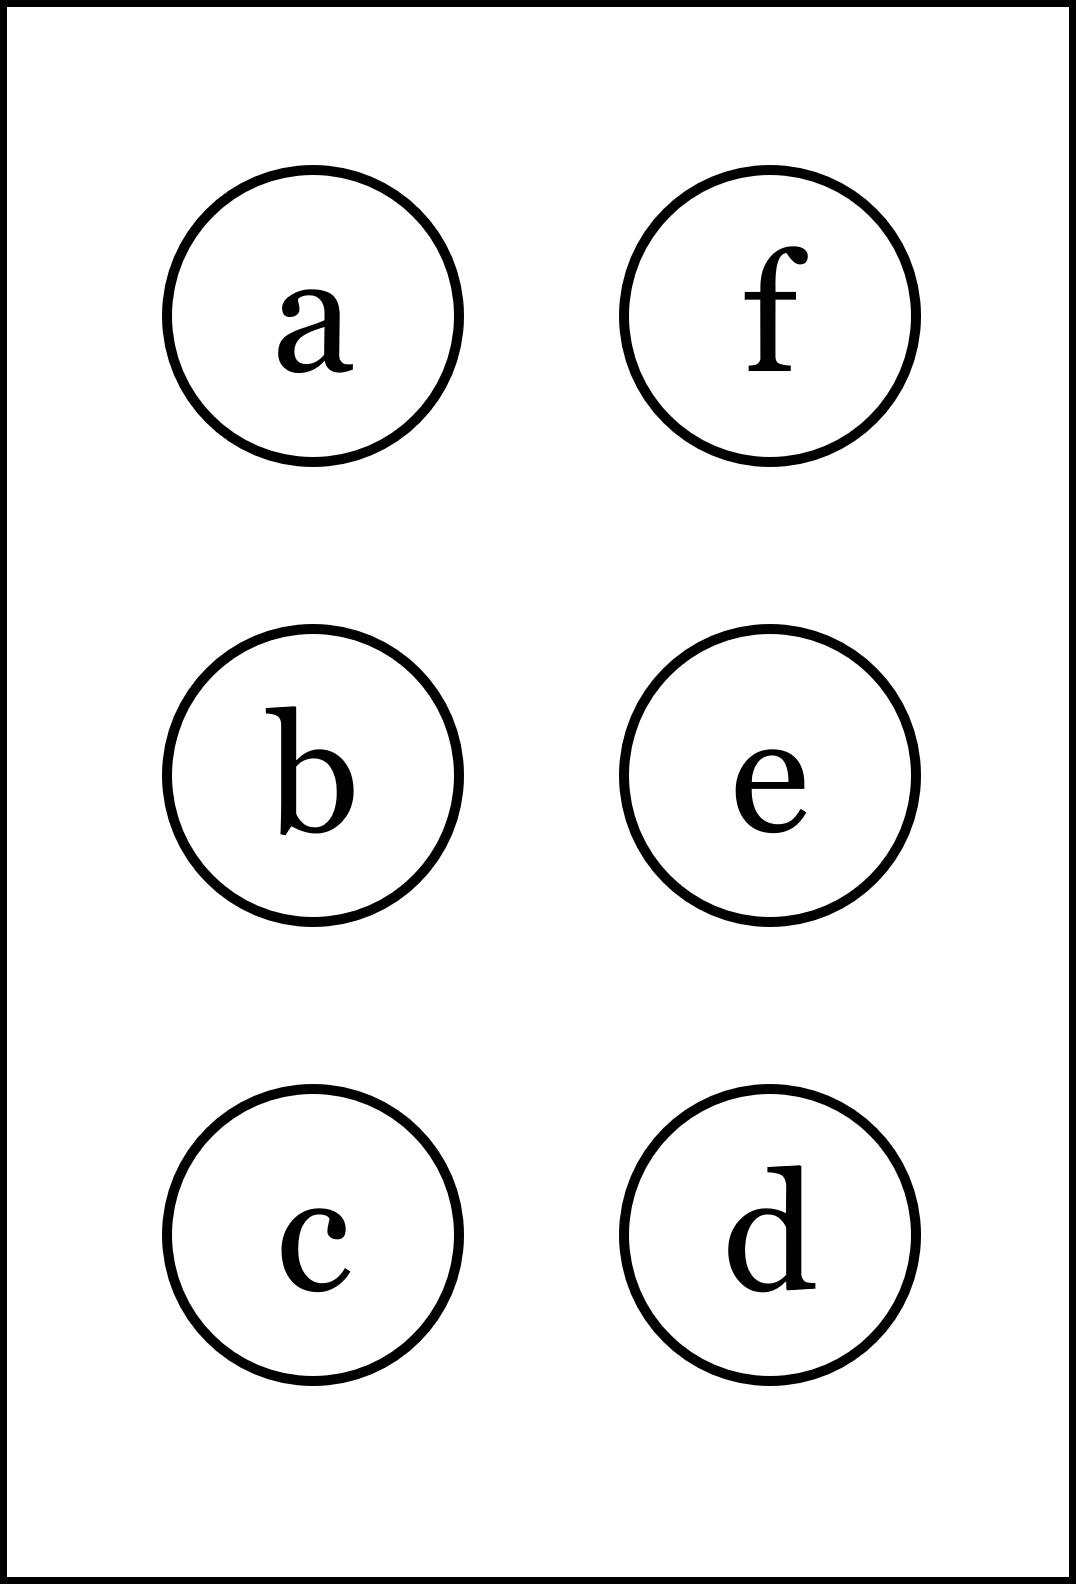
\includegraphics[height=40mm]{../images/braille.png}
{\small Písmeno Braillovej abecedy}
\end{center}
\end{minipage}
\end{center}
\end{minipage}
%
\end{tabular}
\newpage
\thispagestyle{empty}
\begin{tabular}{c:c}
\begin{minipage}[c][104.5mm][t]{0.5\linewidth}
\begin{center}
\vspace{7mm}
{\huge Kvadratická rovnice, skupina \textit{Gamma $\gamma$} -\romannumeral1}\\[5mm]
\textit{Jméno:}\phantom{xxxxxxxxxxxxxxxxxxxxxxxxxxxxxxxxxxxxxxxxxxxxxxxxxxxxxxxxxxxxxxxxx}\\[5mm]
\begin{minipage}{0.95\linewidth}
\begin{center}
V \textbf{(a)} a \textbf{(b)} zjisti počet řešení. V \textbf{(c)} x-ovú polohu vrcholu, a v \textbf{(d)} y-ovú polohu vrcholu.\\V \textbf{(e)} a \textbf{(f)} zjisti součet řešení. Pokud ti vyjde stejný výsledek jako je za otazníky, tak\\napravo obarvi příslušející kroužek načerno. \textbf{Spolu odevzdejte výsledné slovo}.
\end{center}
\end{minipage}
\\[1mm]
\begin{minipage}{0.79\linewidth}
\begin{center}
\begin{varwidth}{\linewidth}
\begin{enumerate}
\Large
\item $3x^2-7x+1=0$\quad \dotfill\; ???\;\dotfill \quad 2
\item $-4x^2+2x+3=0$\quad \dotfill\; ???\;\dotfill \quad 2
\item $f(x)=2x^2+5x+4$\quad \dotfill\; ???\;\dotfill \quad $\nicefrac{-5}{4}$
\item $f(x)=-2x^2+2x-3$\quad \dotfill\; ???\;\dotfill \quad $\nicefrac{-5}{2}$
\item $-4x^2-12x-8=0$\quad \dotfill\; ???\;\dotfill \quad -4
\item $-15x^2-4x+3=0$\quad \dotfill\; ???\;\dotfill \quad $\nicefrac{14}{15}$
\end{enumerate}
\end{varwidth}
\end{center}
\end{minipage}
\begin{minipage}{0.20\linewidth}
\begin{center}
{\Huge\bfseries 1.} \\[2mm]
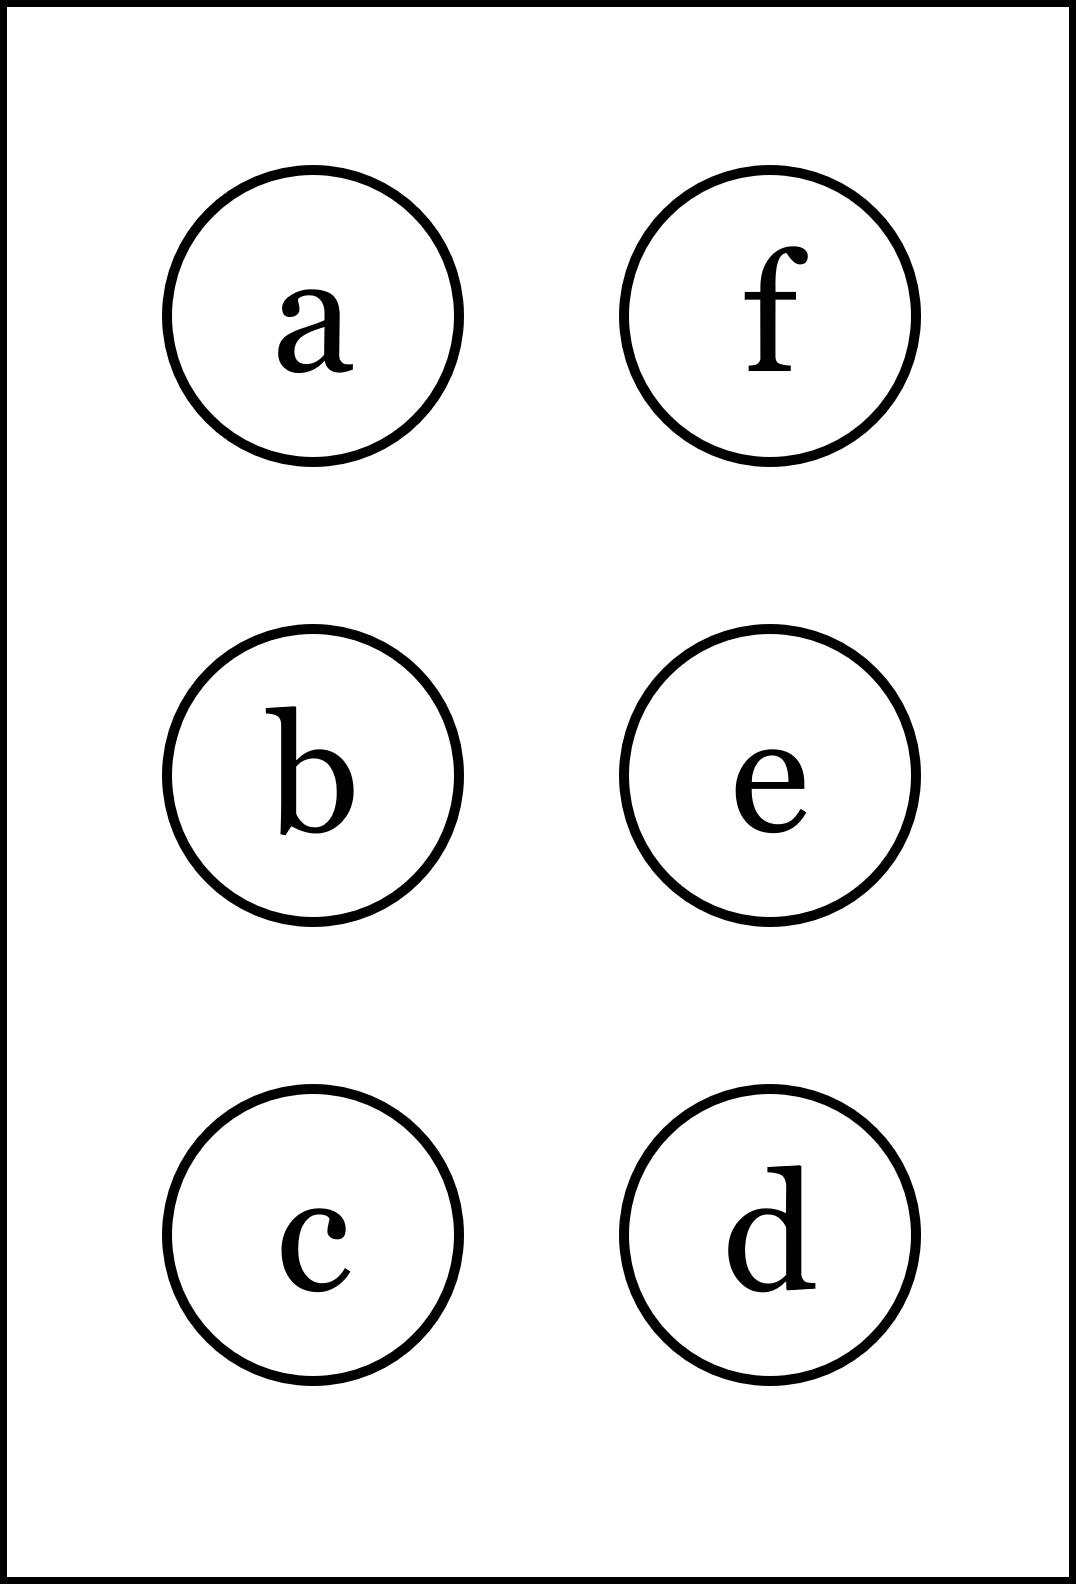
\includegraphics[height=40mm]{../images/braille.png}
{\small Písmeno Braillovej abecedy}
\end{center}
\end{minipage}
\end{center}
\end{minipage}
&
\begin{minipage}[c][104.5mm][t]{0.5\linewidth}
\begin{center}
\vspace{7mm}
{\huge Kvadratická rovnice, skupina \textit{Gamma $\gamma$} -\romannumeral2}\\[5mm]
\textit{Jméno:}\phantom{xxxxxxxxxxxxxxxxxxxxxxxxxxxxxxxxxxxxxxxxxxxxxxxxxxxxxxxxxxxxxxxxx}\\[5mm]
\begin{minipage}{0.95\linewidth}
\begin{center}
V \textbf{(a)} a \textbf{(b)} zjisti počet řešení. V \textbf{(c)} x-ovú polohu vrcholu, a v \textbf{(d)} y-ovú polohu vrcholu.\\V \textbf{(e)} a \textbf{(f)} zjisti součet řešení. Pokud ti vyjde stejný výsledek jako je za otazníky, tak\\napravo obarvi příslušející kroužek načerno. \textbf{Spolu odevzdejte výsledné slovo}.
\end{center}
\end{minipage}
\\[1mm]
\begin{minipage}{0.79\linewidth}
\begin{center}
\begin{varwidth}{\linewidth}
\begin{enumerate}
\Large
\item $3x^2+2x-1=0$\quad \dotfill\; ???\;\dotfill \quad 2
\item $-8x^2-4x+1=0$\quad \dotfill\; ???\;\dotfill \quad 0
\item $f(x)=-x^2-3x+3$\quad \dotfill\; ???\;\dotfill \quad $\nicefrac{3}{2}$
\item $f(x)=2x^2-6x+4$\quad \dotfill\; ???\;\dotfill \quad $\nicefrac{-5}{2}$
\item $-x^2-5x-6=0$\quad \dotfill\; ???\;\dotfill \quad -8
\item $2x^2-6x-20=0$\quad \dotfill\; ???\;\dotfill \quad $7$
\end{enumerate}
\end{varwidth}
\end{center}
\end{minipage}
\begin{minipage}{0.20\linewidth}
\begin{center}
{\Huge\bfseries 2.} \\[2mm]
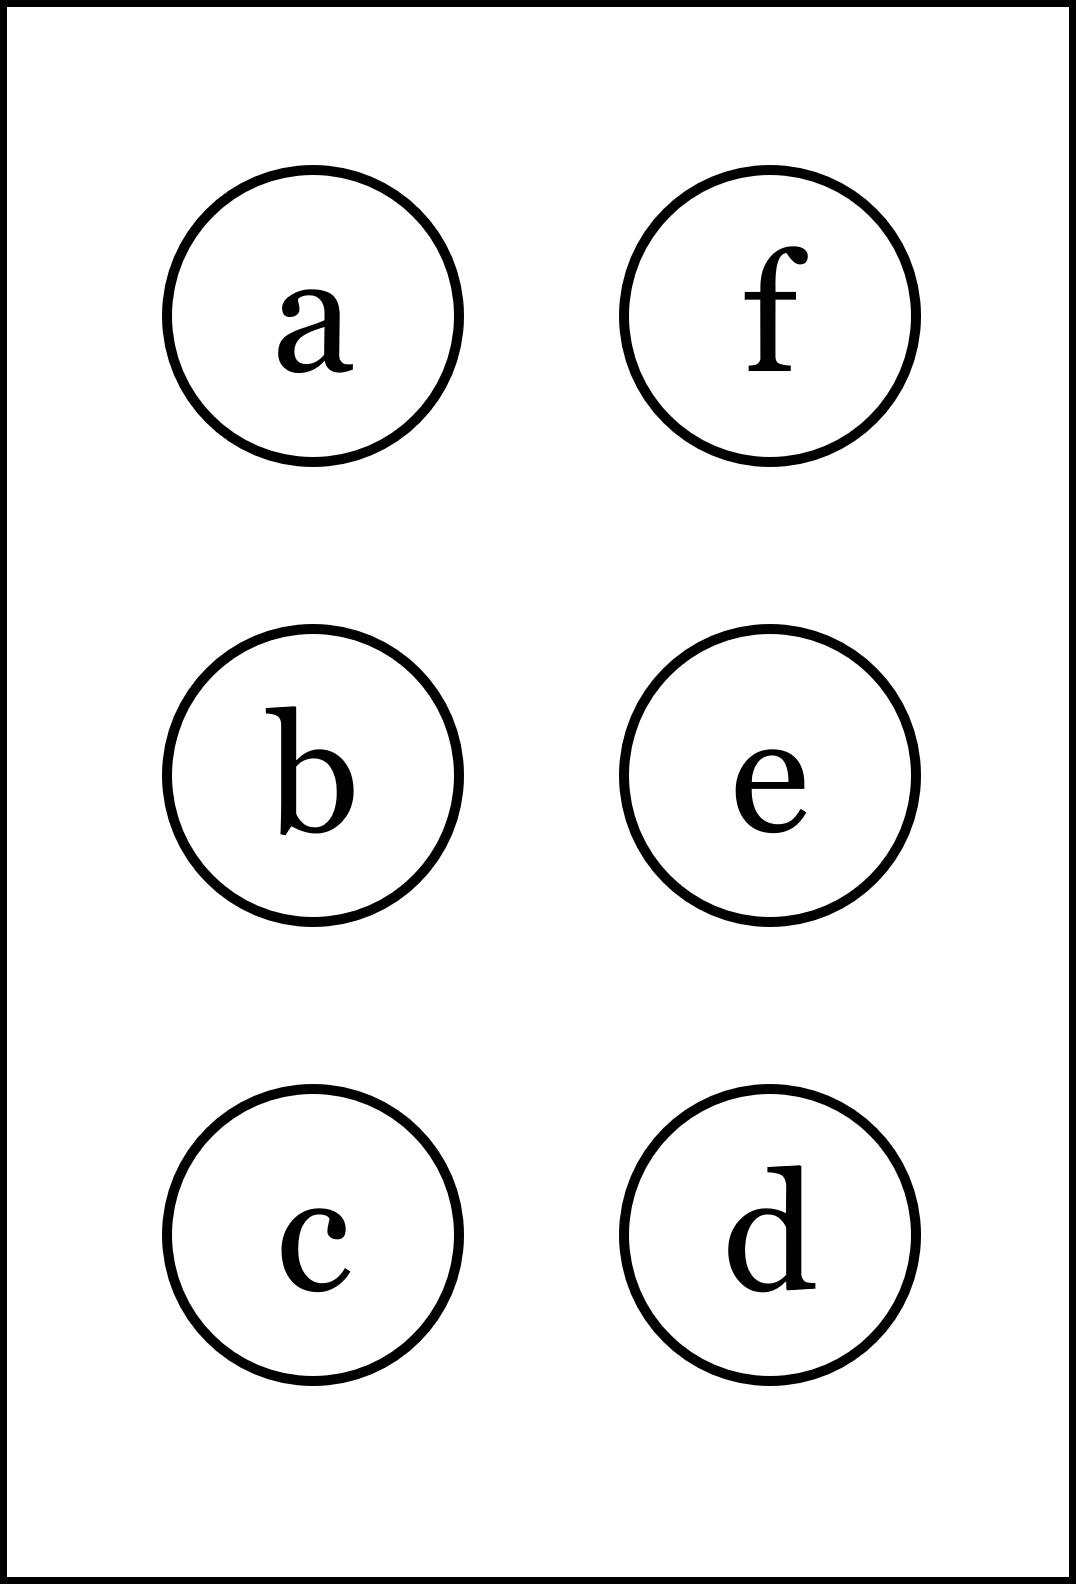
\includegraphics[height=40mm]{../images/braille.png}
{\small Písmeno Braillovej abecedy}
\end{center}
\end{minipage}
\end{center}
\end{minipage}
\\ \hdashline
\begin{minipage}[c][104.5mm][t]{0.5\linewidth}
\begin{center}
\vspace{7mm}
{\huge Kvadratická rovnice, skupina \textit{Gamma $\gamma$} -\romannumeral3}\\[5mm]
\textit{Jméno:}\phantom{xxxxxxxxxxxxxxxxxxxxxxxxxxxxxxxxxxxxxxxxxxxxxxxxxxxxxxxxxxxxxxxxx}\\[5mm]
\begin{minipage}{0.95\linewidth}
\begin{center}
V \textbf{(a)} a \textbf{(b)} zjisti počet řešení. V \textbf{(c)} x-ovú polohu vrcholu, a v \textbf{(d)} y-ovú polohu vrcholu.\\V \textbf{(e)} a \textbf{(f)} zjisti součet řešení. Pokud ti vyjde stejný výsledek jako je za otazníky, tak\\napravo obarvi příslušející kroužek načerno. \textbf{Spolu odevzdejte výsledné slovo}.
\end{center}
\end{minipage}
\\[1mm]
\begin{minipage}{0.79\linewidth}
\begin{center}
\begin{varwidth}{\linewidth}
\begin{enumerate}
\Large
\item $6x^2-x+3=0$\quad \dotfill\; ???\;\dotfill \quad 0
\item $-2x^2-6x-4=0$\quad \dotfill\; ???\;\dotfill \quad 1
\item $f(x)=-5x^2+5x+1$\quad \dotfill\; ???\;\dotfill \quad $\nicefrac{1}{2}$
\item $f(x)=-3x^2+x-6$\quad \dotfill\; ???\;\dotfill \quad $\nicefrac{-35}{12}$
\item $2x^2+16x+14=0$\quad \dotfill\; ???\;\dotfill \quad -8
\item $-12x^2+10x-2=0$\quad \dotfill\; ???\;\dotfill \quad $\nicefrac{5}{6}$
\end{enumerate}
\end{varwidth}
\end{center}
\end{minipage}
\begin{minipage}{0.20\linewidth}
\begin{center}
{\Huge\bfseries 3.} \\[2mm]
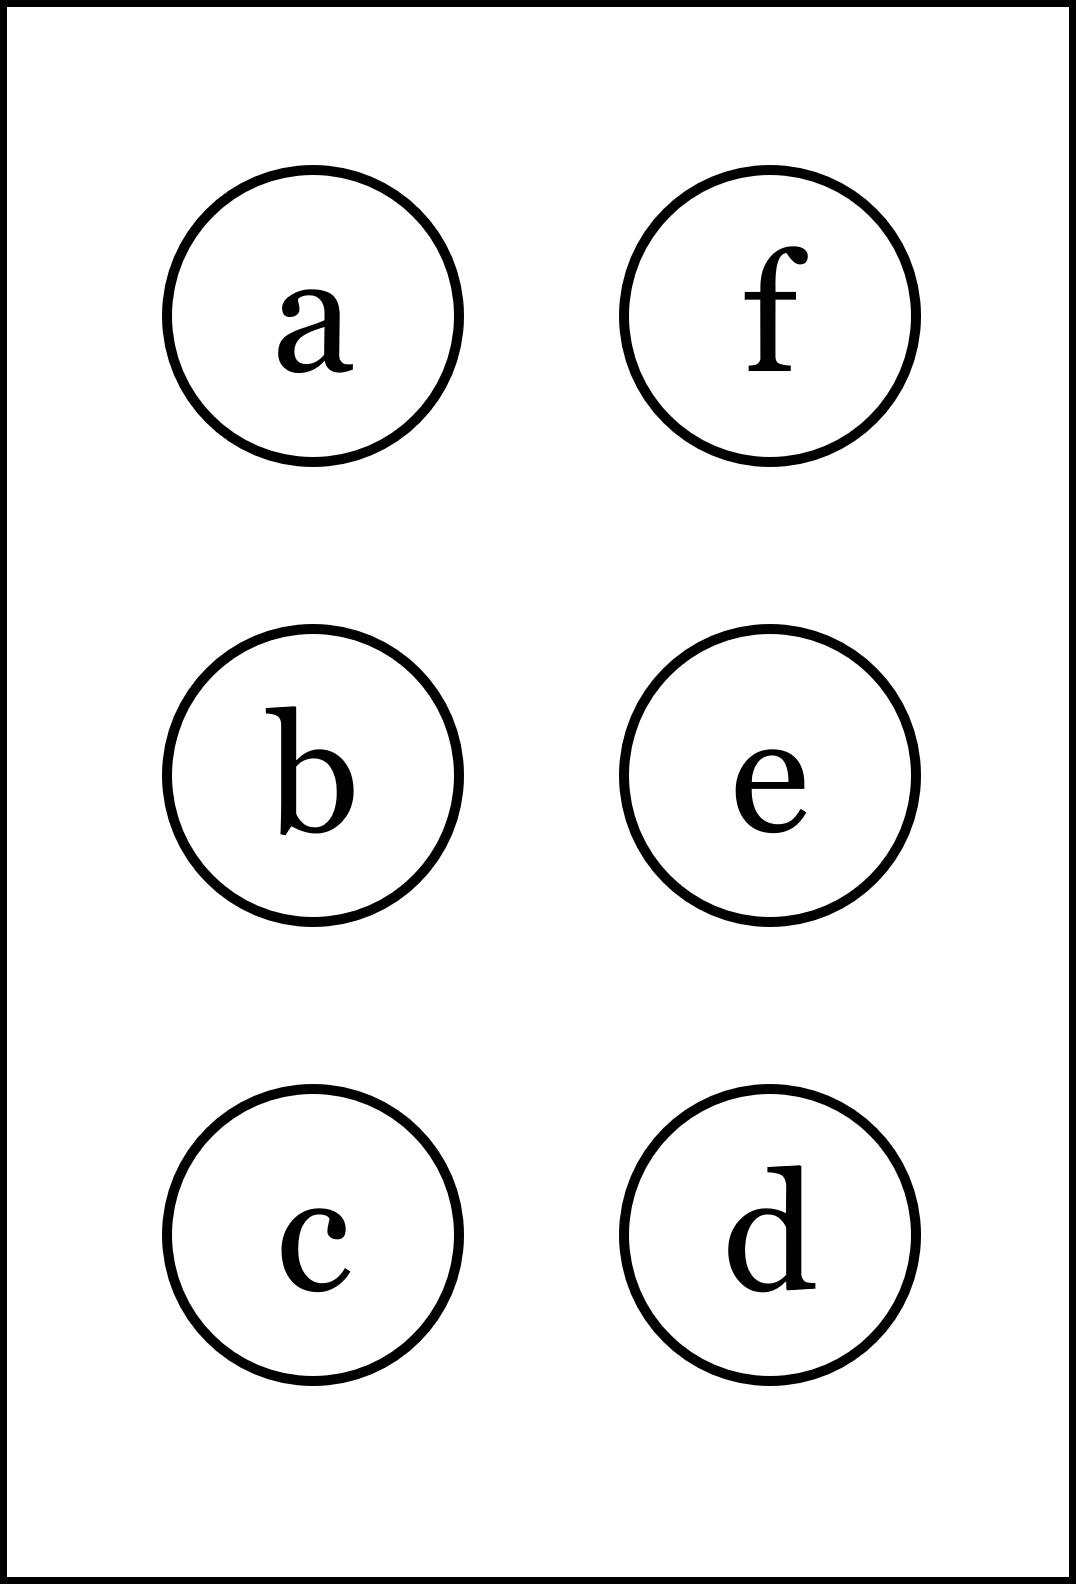
\includegraphics[height=40mm]{../images/braille.png}
{\small Písmeno Braillovej abecedy}
\end{center}
\end{minipage}
\end{center}
\end{minipage}
&
\begin{minipage}[c][104.5mm][t]{0.5\linewidth}
\begin{center}
\vspace{7mm}
{\huge Kvadratická rovnice, skupina \textit{Gamma $\gamma$} -\romannumeral4}\\[5mm]
\textit{Jméno:}\phantom{xxxxxxxxxxxxxxxxxxxxxxxxxxxxxxxxxxxxxxxxxxxxxxxxxxxxxxxxxxxxxxxxx}\\[5mm]
\begin{minipage}{0.95\linewidth}
\begin{center}
V \textbf{(a)} a \textbf{(b)} zjisti počet řešení. V \textbf{(c)} x-ovú polohu vrcholu, a v \textbf{(d)} y-ovú polohu vrcholu.\\V \textbf{(e)} a \textbf{(f)} zjisti součet řešení. Pokud ti vyjde stejný výsledek jako je za otazníky, tak\\napravo obarvi příslušející kroužek načerno. \textbf{Spolu odevzdejte výsledné slovo}.
\end{center}
\end{minipage}
\\[1mm]
\begin{minipage}{0.79\linewidth}
\begin{center}
\begin{varwidth}{\linewidth}
\begin{enumerate}
\Large
\item $2x^2-x-2=0$\quad \dotfill\; ???\;\dotfill \quad 2
\item $-2x^2+x-2=0$\quad \dotfill\; ???\;\dotfill \quad 2
\item $f(x)=5x^2+2x+4$\quad \dotfill\; ???\;\dotfill \quad $\nicefrac{1}{5}$
\item $f(x)=-2x^2-x+2$\quad \dotfill\; ???\;\dotfill \quad $\nicefrac{9}{8}$
\item $x^2+3x-28=0$\quad \dotfill\; ???\;\dotfill \quad -6
\item $8x^2-12x+4=0$\quad \dotfill\; ???\;\dotfill \quad $\nicefrac{1}{2}$
\end{enumerate}
\end{varwidth}
\end{center}
\end{minipage}
\begin{minipage}{0.20\linewidth}
\begin{center}
{\Huge\bfseries 4.} \\[2mm]
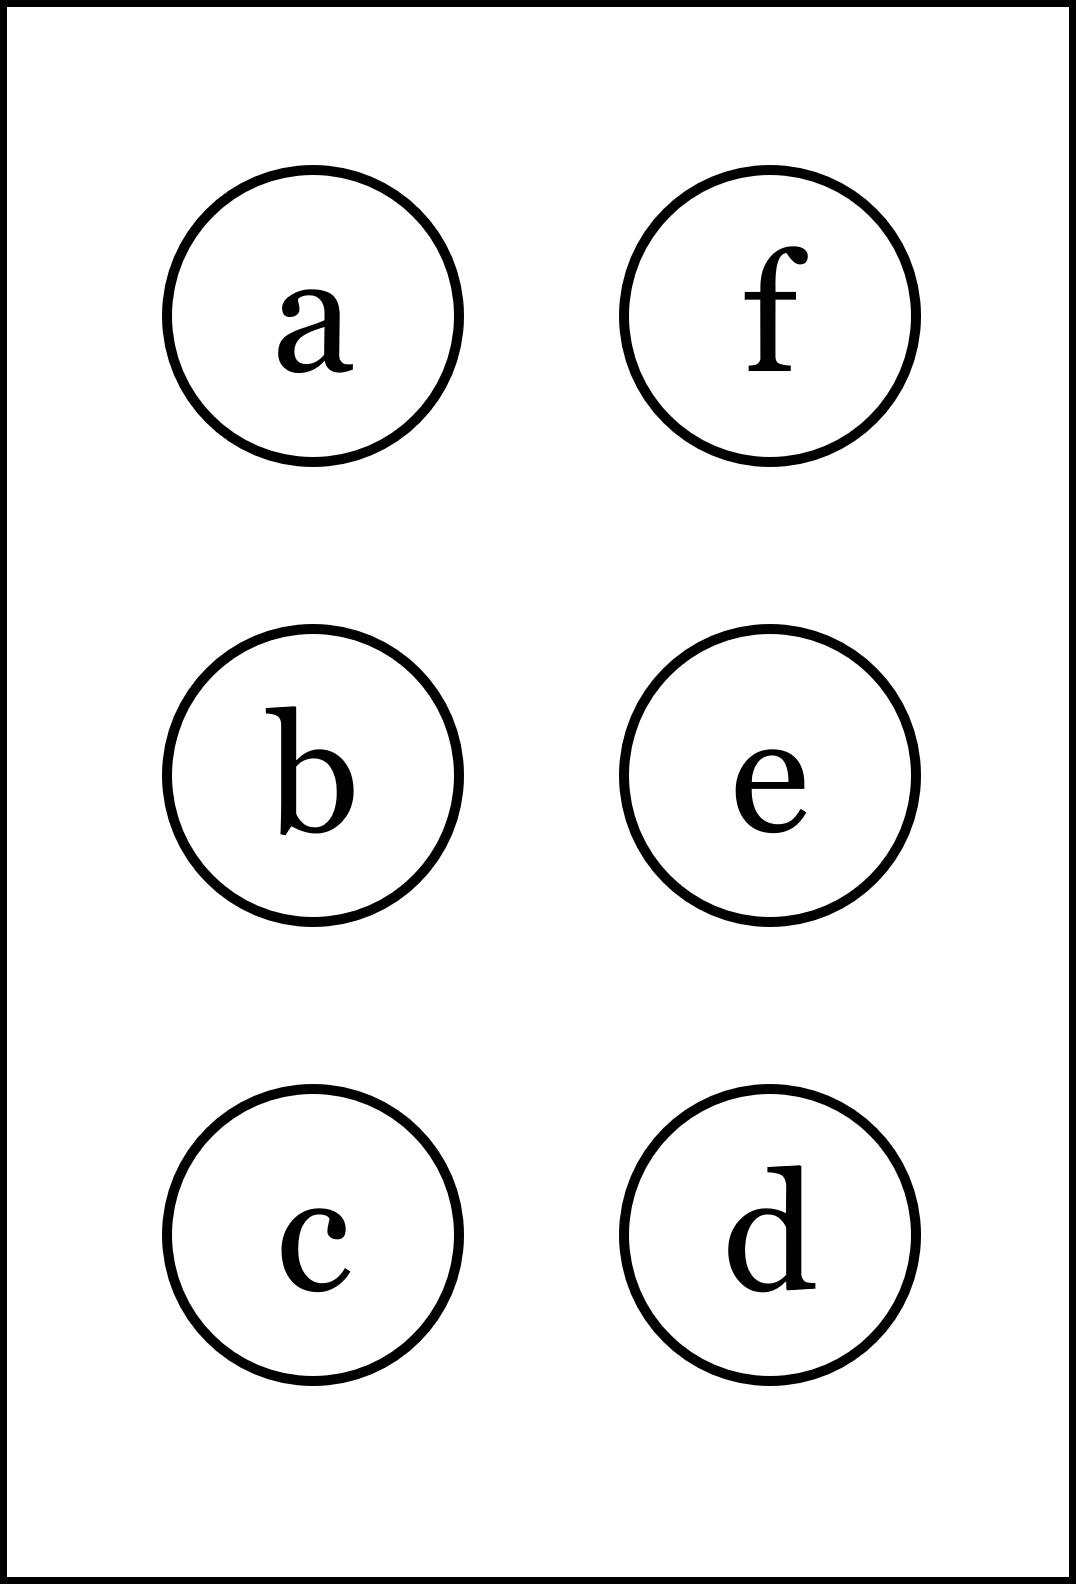
\includegraphics[height=40mm]{../images/braille.png}
{\small Písmeno Braillovej abecedy}
\end{center}
\end{minipage}
\end{center}
\end{minipage}
%
\end{tabular}
\newpage
\thispagestyle{empty}
\begin{tabular}{c:c}
\begin{minipage}[c][104.5mm][t]{0.5\linewidth}
\begin{center}
\vspace{7mm}
{\huge Kvadratická rovnice, skupina \textit{Delta $\delta$} -\romannumeral1}\\[5mm]
\textit{Jméno:}\phantom{xxxxxxxxxxxxxxxxxxxxxxxxxxxxxxxxxxxxxxxxxxxxxxxxxxxxxxxxxxxxxxxxx}\\[5mm]
\begin{minipage}{0.95\linewidth}
\begin{center}
V \textbf{(a)} a \textbf{(b)} zjisti počet řešení. V \textbf{(c)} x-ovú polohu vrcholu, a v \textbf{(d)} y-ovú polohu vrcholu.\\V \textbf{(e)} a \textbf{(f)} zjisti součet řešení. Pokud ti vyjde stejný výsledek jako je za otazníky, tak\\napravo obarvi příslušející kroužek načerno. \textbf{Spolu odevzdejte výsledné slovo}.
\end{center}
\end{minipage}
\\[1mm]
\begin{minipage}{0.79\linewidth}
\begin{center}
\begin{varwidth}{\linewidth}
\begin{enumerate}
\Large
\item $4x^2+8x-3=0$\quad \dotfill\; ???\;\dotfill \quad 2
\item $-5x^2+3x-2=0$\quad \dotfill\; ???\;\dotfill \quad 1
\item $f(x)=x^2-2x-6$\quad \dotfill\; ???\;\dotfill \quad $-1$
\item $f(x)=-x^2-6x+4$\quad \dotfill\; ???\;\dotfill \quad $11$
\item $-3x^2+21x-30=0$\quad \dotfill\; ???\;\dotfill \quad 5
\item $4x^2-7x-2=0$\quad \dotfill\; ???\;\dotfill \quad $\nicefrac{-9}{4}$
\end{enumerate}
\end{varwidth}
\end{center}
\end{minipage}
\begin{minipage}{0.20\linewidth}
\begin{center}
{\Huge\bfseries 1.} \\[2mm]
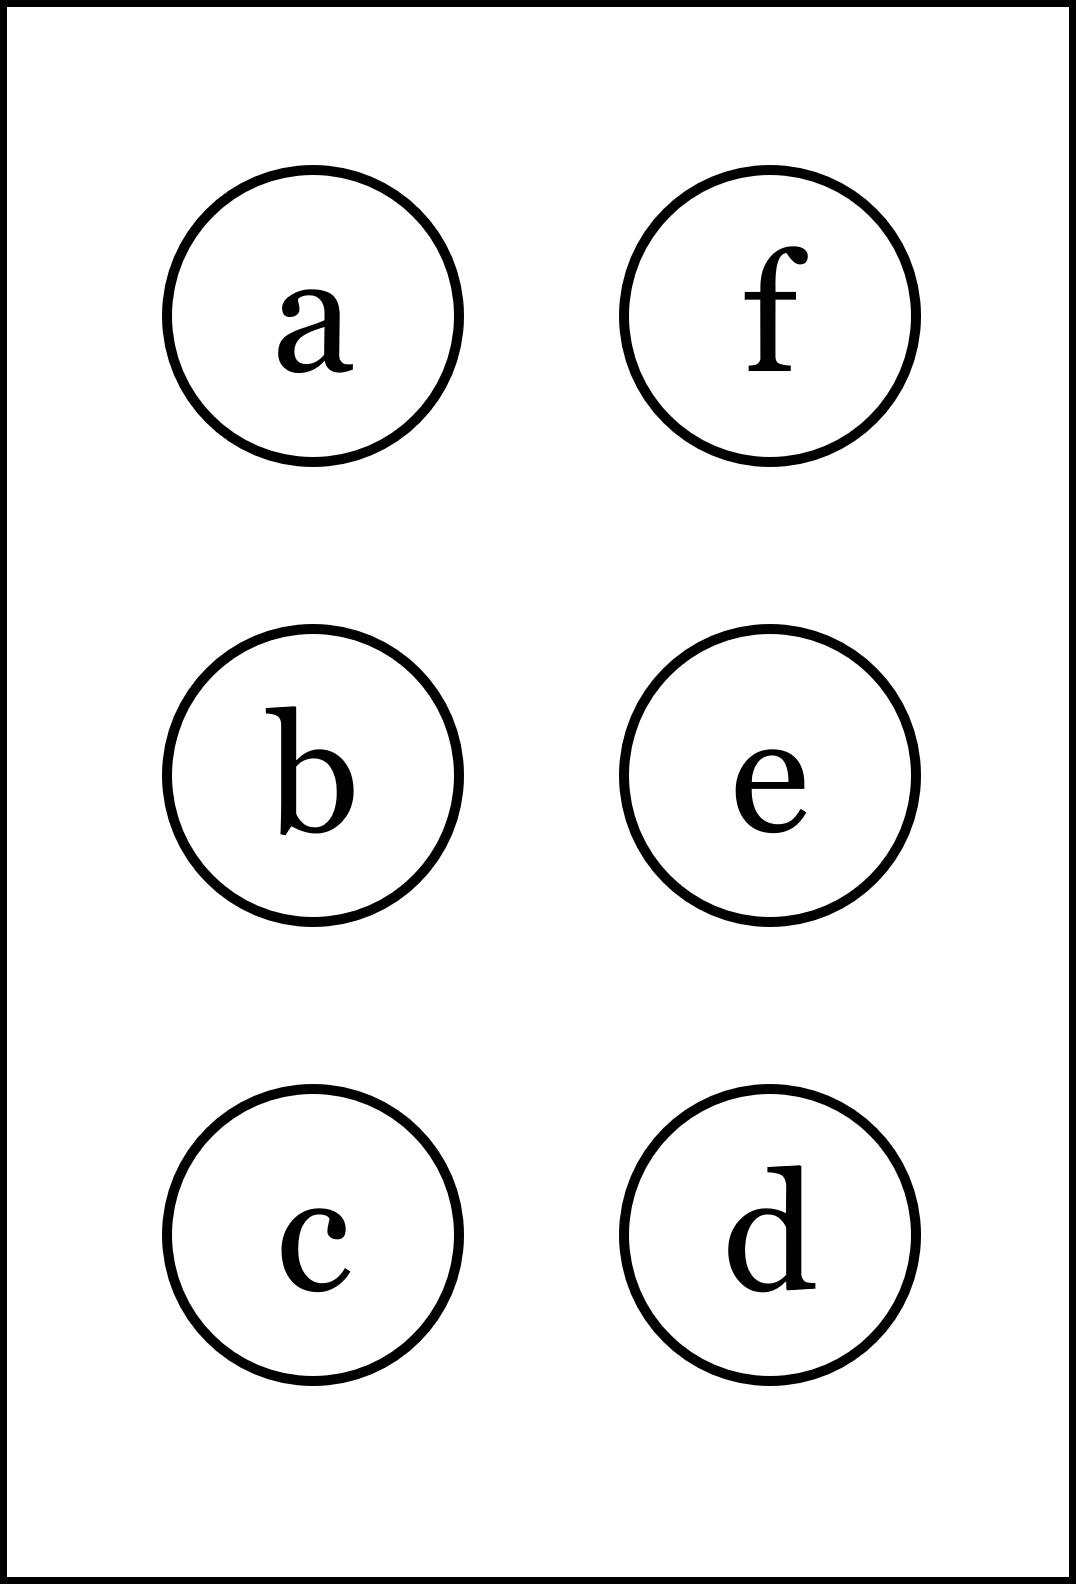
\includegraphics[height=40mm]{../images/braille.png}
{\small Písmeno Braillovej abecedy}
\end{center}
\end{minipage}
\end{center}
\end{minipage}
&
\begin{minipage}[c][104.5mm][t]{0.5\linewidth}
\begin{center}
\vspace{7mm}
{\huge Kvadratická rovnice, skupina \textit{Delta $\delta$} -\romannumeral2}\\[5mm]
\textit{Jméno:}\phantom{xxxxxxxxxxxxxxxxxxxxxxxxxxxxxxxxxxxxxxxxxxxxxxxxxxxxxxxxxxxxxxxxx}\\[5mm]
\begin{minipage}{0.95\linewidth}
\begin{center}
V \textbf{(a)} a \textbf{(b)} zjisti počet řešení. V \textbf{(c)} x-ovú polohu vrcholu, a v \textbf{(d)} y-ovú polohu vrcholu.\\V \textbf{(e)} a \textbf{(f)} zjisti součet řešení. Pokud ti vyjde stejný výsledek jako je za otazníky, tak\\napravo obarvi příslušející kroužek načerno. \textbf{Spolu odevzdejte výsledné slovo}.
\end{center}
\end{minipage}
\\[1mm]
\begin{minipage}{0.79\linewidth}
\begin{center}
\begin{varwidth}{\linewidth}
\begin{enumerate}
\Large
\item $2x^2+4x+1=0$\quad \dotfill\; ???\;\dotfill \quad 2
\item $5x^2+3x-2=0$\quad \dotfill\; ???\;\dotfill \quad 1
\item $f(x)=-6x^2-8x-3$\quad \dotfill\; ???\;\dotfill \quad $\nicefrac{-2}{3}$
\item $f(x)=4x^2-3x+2$\quad \dotfill\; ???\;\dotfill \quad $\nicefrac{23}{16}$
\item $-8x^2+24x-16=0$\quad \dotfill\; ???\;\dotfill \quad 5
\item $7x^2+12x+5=0$\quad \dotfill\; ???\;\dotfill \quad $\nicefrac{-2}{7}$
\end{enumerate}
\end{varwidth}
\end{center}
\end{minipage}
\begin{minipage}{0.20\linewidth}
\begin{center}
{\Huge\bfseries 2.} \\[2mm]
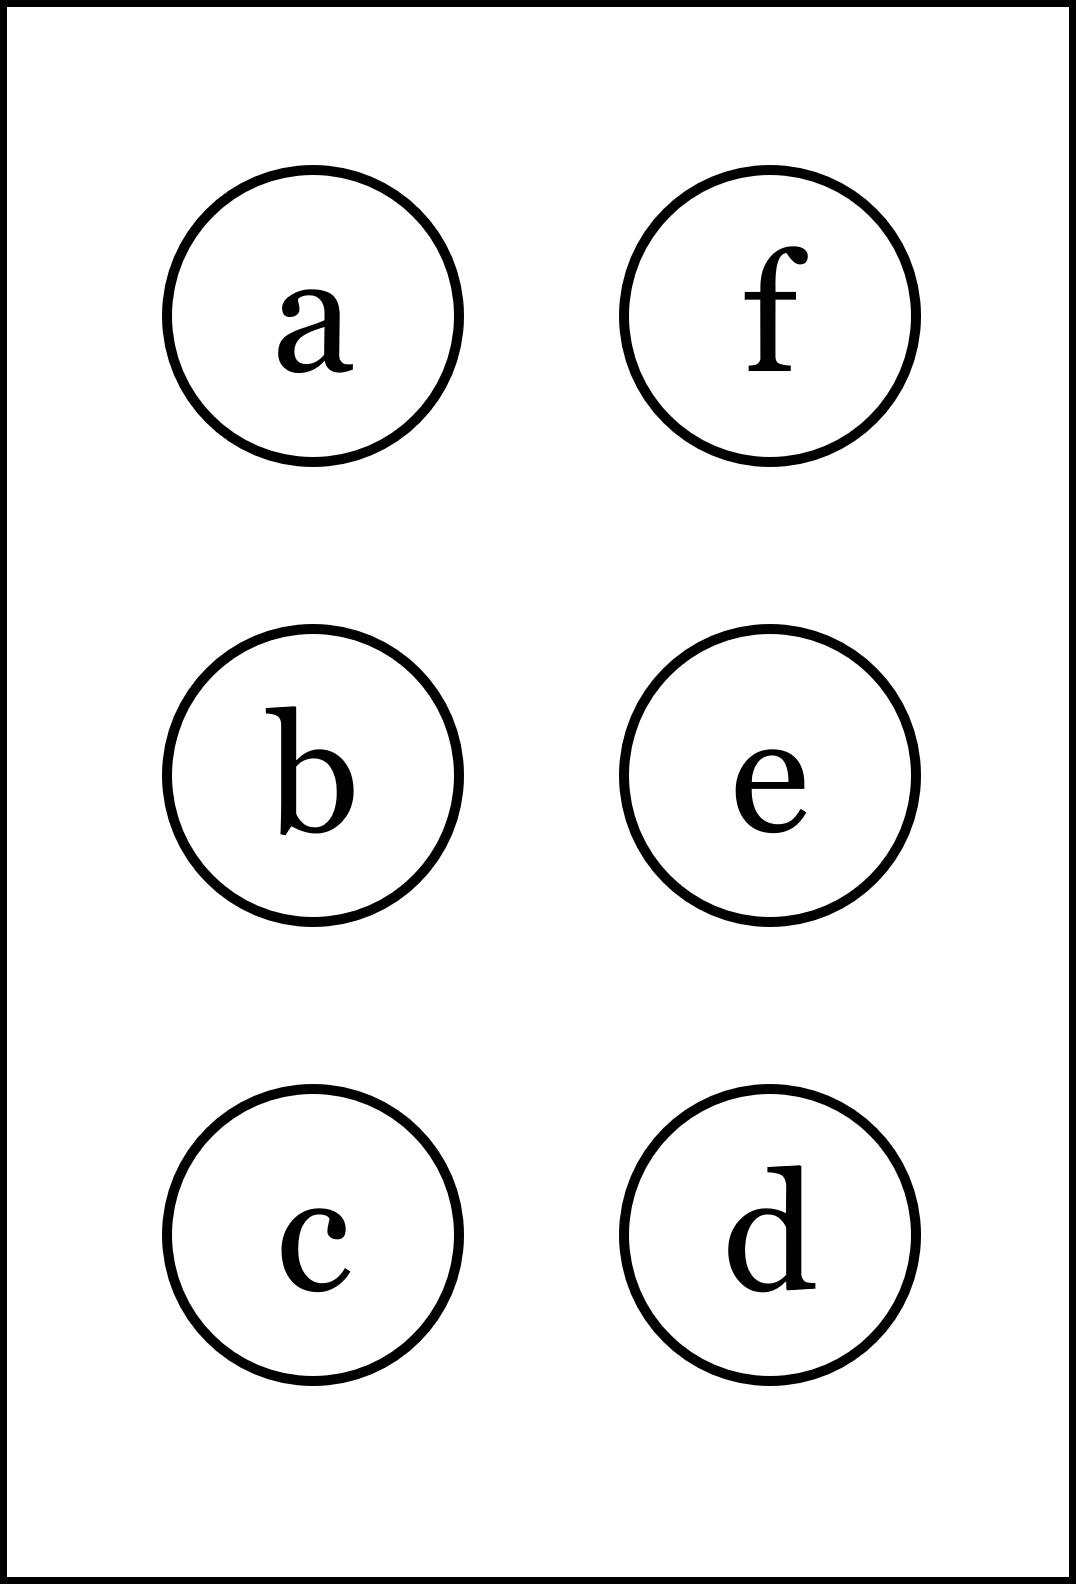
\includegraphics[height=40mm]{../images/braille.png}
{\small Písmeno Braillovej abecedy}
\end{center}
\end{minipage}
\end{center}
\end{minipage}
\\ \hdashline
\begin{minipage}[c][104.5mm][t]{0.5\linewidth}
\begin{center}
\vspace{7mm}
{\huge Kvadratická rovnice, skupina \textit{Delta $\delta$} -\romannumeral3}\\[5mm]
\textit{Jméno:}\phantom{xxxxxxxxxxxxxxxxxxxxxxxxxxxxxxxxxxxxxxxxxxxxxxxxxxxxxxxxxxxxxxxxx}\\[5mm]
\begin{minipage}{0.95\linewidth}
\begin{center}
V \textbf{(a)} a \textbf{(b)} zjisti počet řešení. V \textbf{(c)} x-ovú polohu vrcholu, a v \textbf{(d)} y-ovú polohu vrcholu.\\V \textbf{(e)} a \textbf{(f)} zjisti součet řešení. Pokud ti vyjde stejný výsledek jako je za otazníky, tak\\napravo obarvi příslušející kroužek načerno. \textbf{Spolu odevzdejte výsledné slovo}.
\end{center}
\end{minipage}
\\[1mm]
\begin{minipage}{0.79\linewidth}
\begin{center}
\begin{varwidth}{\linewidth}
\begin{enumerate}
\Large
\item $3x^2+7x-2=0$\quad \dotfill\; ???\;\dotfill \quad 0
\item $-x^2-x-4=0$\quad \dotfill\; ???\;\dotfill \quad 0
\item $f(x)=2x^2-4x-3$\quad \dotfill\; ???\;\dotfill \quad $1$
\item $f(x)=6x^2-7x-2$\quad \dotfill\; ???\;\dotfill \quad $\nicefrac{-73}{24}$
\item $-3x^2-12x-9=0$\quad \dotfill\; ???\;\dotfill \quad -4
\item $2x^2+8x+6=0$\quad \dotfill\; ???\;\dotfill \quad $-4$
\end{enumerate}
\end{varwidth}
\end{center}
\end{minipage}
\begin{minipage}{0.20\linewidth}
\begin{center}
{\Huge\bfseries 3.} \\[2mm]
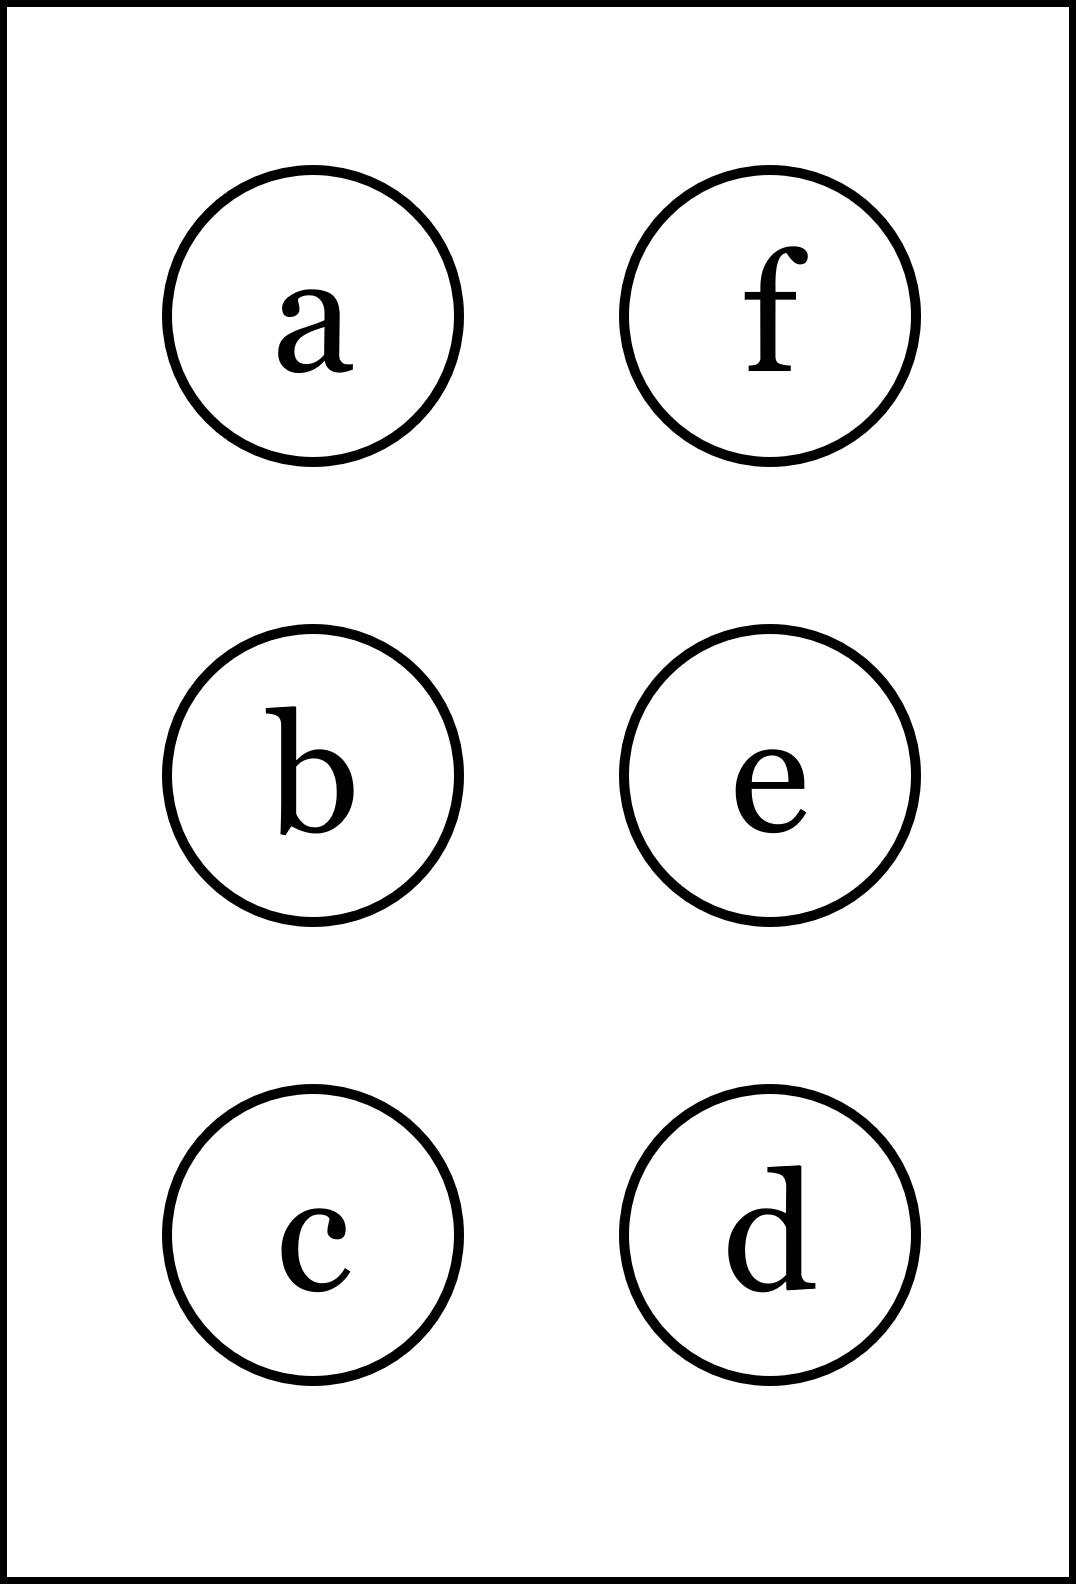
\includegraphics[height=40mm]{../images/braille.png}
{\small Písmeno Braillovej abecedy}
\end{center}
\end{minipage}
\end{center}
\end{minipage}
&
\begin{minipage}[c][104.5mm][t]{0.5\linewidth}
\begin{center}
\vspace{7mm}
{\huge Kvadratická rovnice, skupina \textit{Delta $\delta$} -\romannumeral4}\\[5mm]
\textit{Jméno:}\phantom{xxxxxxxxxxxxxxxxxxxxxxxxxxxxxxxxxxxxxxxxxxxxxxxxxxxxxxxxxxxxxxxxx}\\[5mm]
\begin{minipage}{0.95\linewidth}
\begin{center}
V \textbf{(a)} a \textbf{(b)} zjisti počet řešení. V \textbf{(c)} x-ovú polohu vrcholu, a v \textbf{(d)} y-ovú polohu vrcholu.\\V \textbf{(e)} a \textbf{(f)} zjisti součet řešení. Pokud ti vyjde stejný výsledek jako je za otazníky, tak\\napravo obarvi příslušející kroužek načerno. \textbf{Spolu odevzdejte výsledné slovo}.
\end{center}
\end{minipage}
\\[1mm]
\begin{minipage}{0.79\linewidth}
\begin{center}
\begin{varwidth}{\linewidth}
\begin{enumerate}
\Large
\item $2x^2+7x-5=0$\quad \dotfill\; ???\;\dotfill \quad 2
\item $-7x^2+4x+7=0$\quad \dotfill\; ???\;\dotfill \quad 1
\item $f(x)=-8x^2+5x-8$\quad \dotfill\; ???\;\dotfill \quad $\nicefrac{5}{16}$
\item $f(x)=6x^2+6x-6$\quad \dotfill\; ???\;\dotfill \quad $\nicefrac{-9}{2}$
\item $4x^2+4x-8=0$\quad \dotfill\; ???\;\dotfill \quad -1
\item $4x^2+4x-8=0$\quad \dotfill\; ???\;\dotfill \quad $3$
\end{enumerate}
\end{varwidth}
\end{center}
\end{minipage}
\begin{minipage}{0.20\linewidth}
\begin{center}
{\Huge\bfseries 4.} \\[2mm]
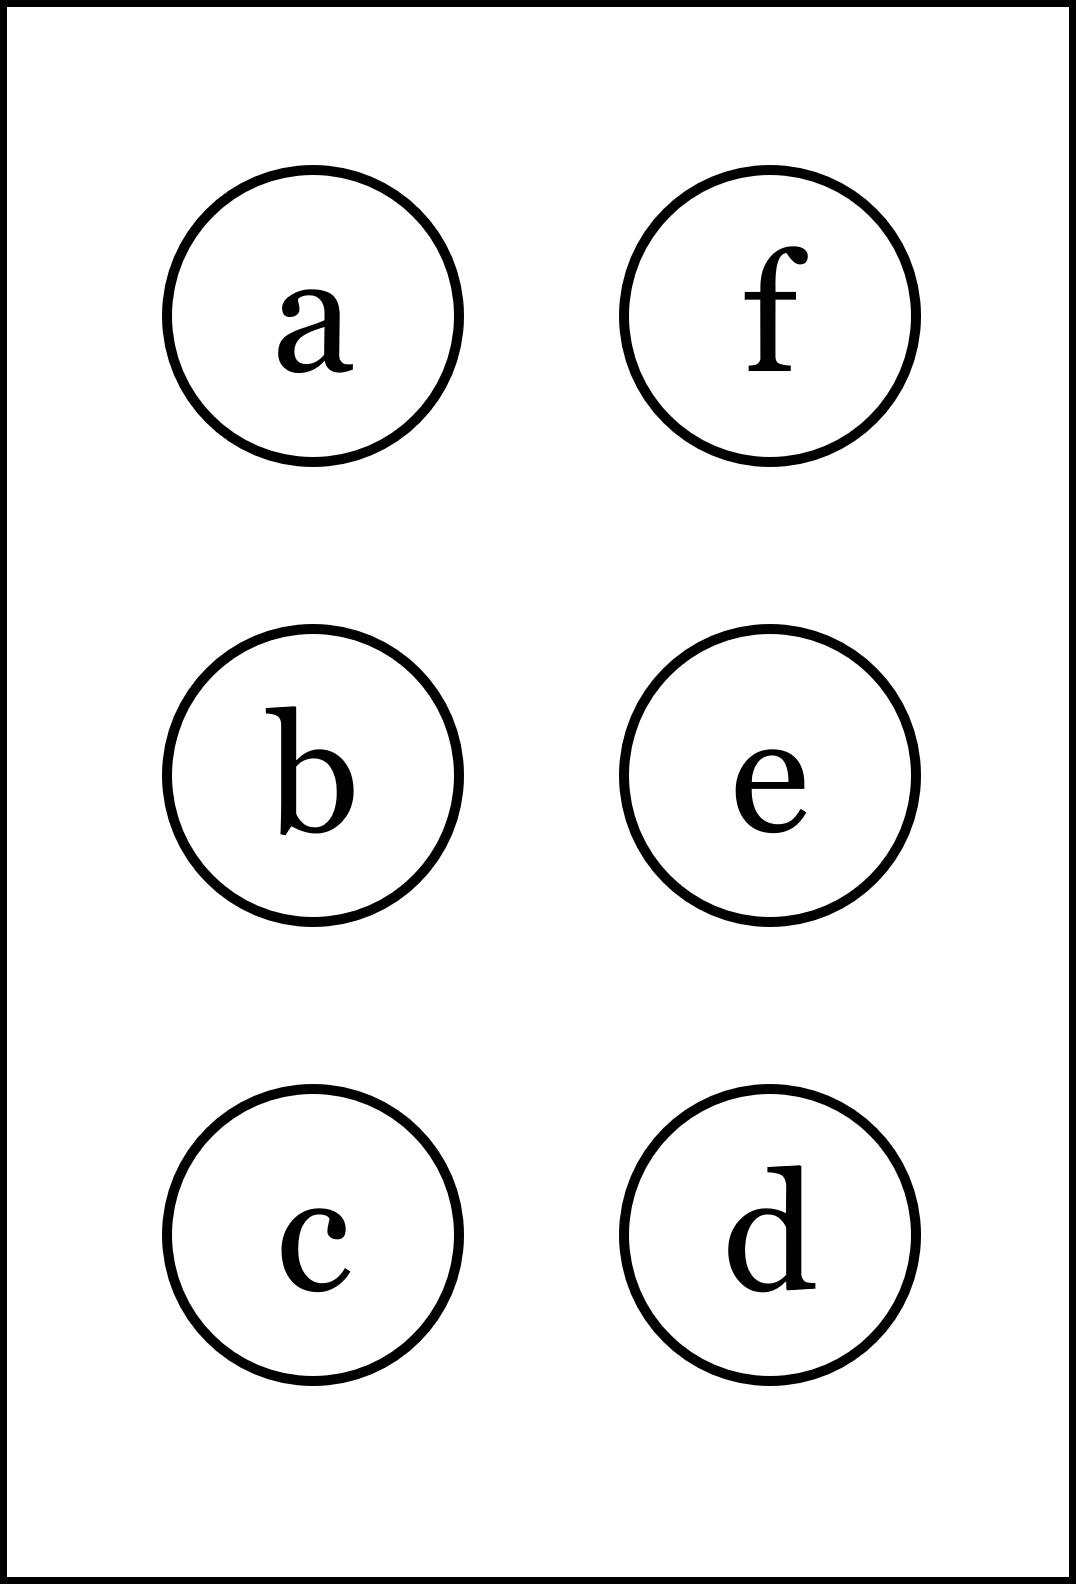
\includegraphics[height=40mm]{../images/braille.png}
{\small Písmeno Braillovej abecedy}
\end{center}
\end{minipage}
\end{center}
\end{minipage}
%
\end{tabular}
\newpage
\thispagestyle{empty}
\begin{tabular}{c:c}
\begin{minipage}[c][104.5mm][t]{0.5\linewidth}
\begin{center}
\vspace{7mm}
{\huge Kvadratická rovnice, skupina \textit{Epsilon $\epsilon$} -\romannumeral1}\\[5mm]
\textit{Jméno:}\phantom{xxxxxxxxxxxxxxxxxxxxxxxxxxxxxxxxxxxxxxxxxxxxxxxxxxxxxxxxxxxxxxxxx}\\[5mm]
\begin{minipage}{0.95\linewidth}
\begin{center}
V \textbf{(a)} a \textbf{(b)} zjisti počet řešení. V \textbf{(c)} x-ovú polohu vrcholu, a v \textbf{(d)} y-ovú polohu vrcholu.\\V \textbf{(e)} a \textbf{(f)} zjisti součet řešení. Pokud ti vyjde stejný výsledek jako je za otazníky, tak\\napravo obarvi příslušející kroužek načerno. \textbf{Spolu odevzdejte výsledné slovo}.
\end{center}
\end{minipage}
\\[1mm]
\begin{minipage}{0.79\linewidth}
\begin{center}
\begin{varwidth}{\linewidth}
\begin{enumerate}
\Large
\item $-3x^2-x+4=0$\quad \dotfill\; ???\;\dotfill \quad 2
\item $-6x^2+2x-8=0$\quad \dotfill\; ???\;\dotfill \quad 0
\item $f(x)=-2x^2-7x+2$\quad \dotfill\; ???\;\dotfill \quad $\nicefrac{7}{4}$
\item $f(x)=x^2+4x-1$\quad \dotfill\; ???\;\dotfill \quad $\nicefrac{-9}{2}$
\item $x^2+10x+24=0$\quad \dotfill\; ???\;\dotfill \quad -10
\item $6x^2+x-5=0$\quad \dotfill\; ???\;\dotfill \quad $\nicefrac{-11}{6}$
\end{enumerate}
\end{varwidth}
\end{center}
\end{minipage}
\begin{minipage}{0.20\linewidth}
\begin{center}
{\Huge\bfseries 1.} \\[2mm]
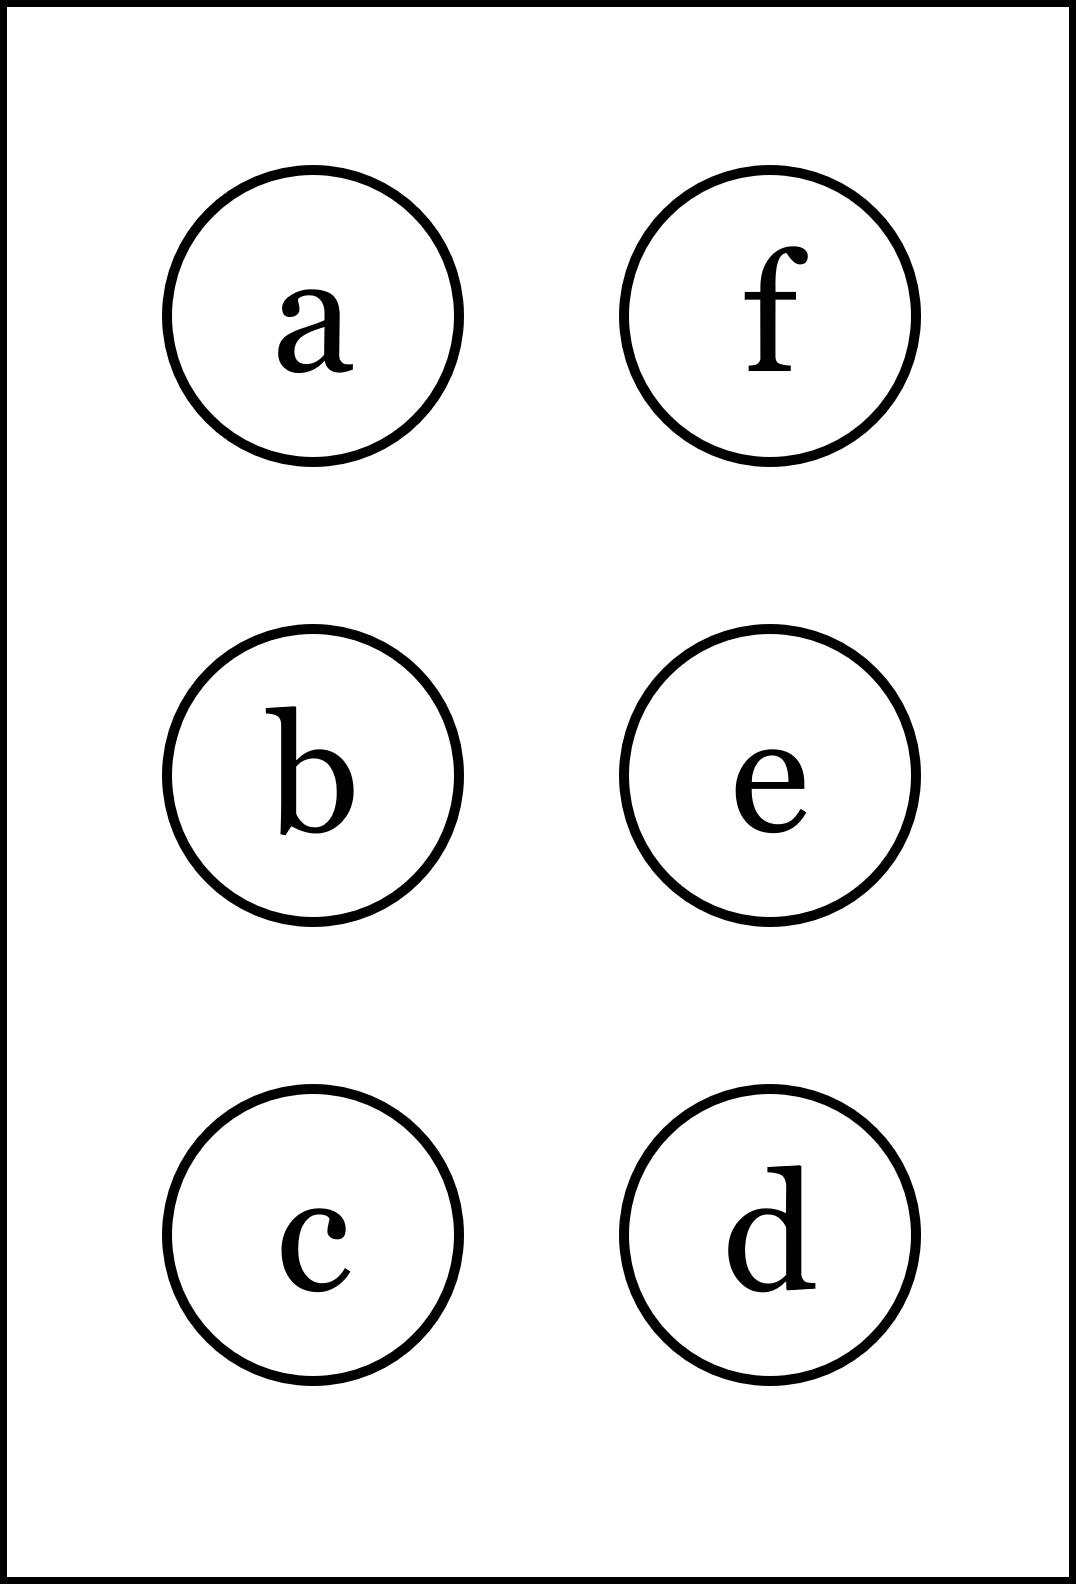
\includegraphics[height=40mm]{../images/braille.png}
{\small Písmeno Braillovej abecedy}
\end{center}
\end{minipage}
\end{center}
\end{minipage}
&
\begin{minipage}[c][104.5mm][t]{0.5\linewidth}
\begin{center}
\vspace{7mm}
{\huge Kvadratická rovnice, skupina \textit{Epsilon $\epsilon$} -\romannumeral2}\\[5mm]
\textit{Jméno:}\phantom{xxxxxxxxxxxxxxxxxxxxxxxxxxxxxxxxxxxxxxxxxxxxxxxxxxxxxxxxxxxxxxxxx}\\[5mm]
\begin{minipage}{0.95\linewidth}
\begin{center}
V \textbf{(a)} a \textbf{(b)} zjisti počet řešení. V \textbf{(c)} x-ovú polohu vrcholu, a v \textbf{(d)} y-ovú polohu vrcholu.\\V \textbf{(e)} a \textbf{(f)} zjisti součet řešení. Pokud ti vyjde stejný výsledek jako je za otazníky, tak\\napravo obarvi příslušející kroužek načerno. \textbf{Spolu odevzdejte výsledné slovo}.
\end{center}
\end{minipage}
\\[1mm]
\begin{minipage}{0.79\linewidth}
\begin{center}
\begin{varwidth}{\linewidth}
\begin{enumerate}
\Large
\item $-5x^2-x-7=0$\quad \dotfill\; ???\;\dotfill \quad 0
\item $x^2+6x+3=0$\quad \dotfill\; ???\;\dotfill \quad 0
\item $f(x)=2x^2+5x-4$\quad \dotfill\; ???\;\dotfill \quad $\nicefrac{-5}{4}$
\item $f(x)=7x^2+5x-3$\quad \dotfill\; ???\;\dotfill \quad $\nicefrac{-67}{28}$
\item $6x^2-18x-24=0$\quad \dotfill\; ???\;\dotfill \quad 3
\item $6x^2-3x-9=0$\quad \dotfill\; ???\;\dotfill \quad $\nicefrac{-5}{2}$
\end{enumerate}
\end{varwidth}
\end{center}
\end{minipage}
\begin{minipage}{0.20\linewidth}
\begin{center}
{\Huge\bfseries 2.} \\[2mm]
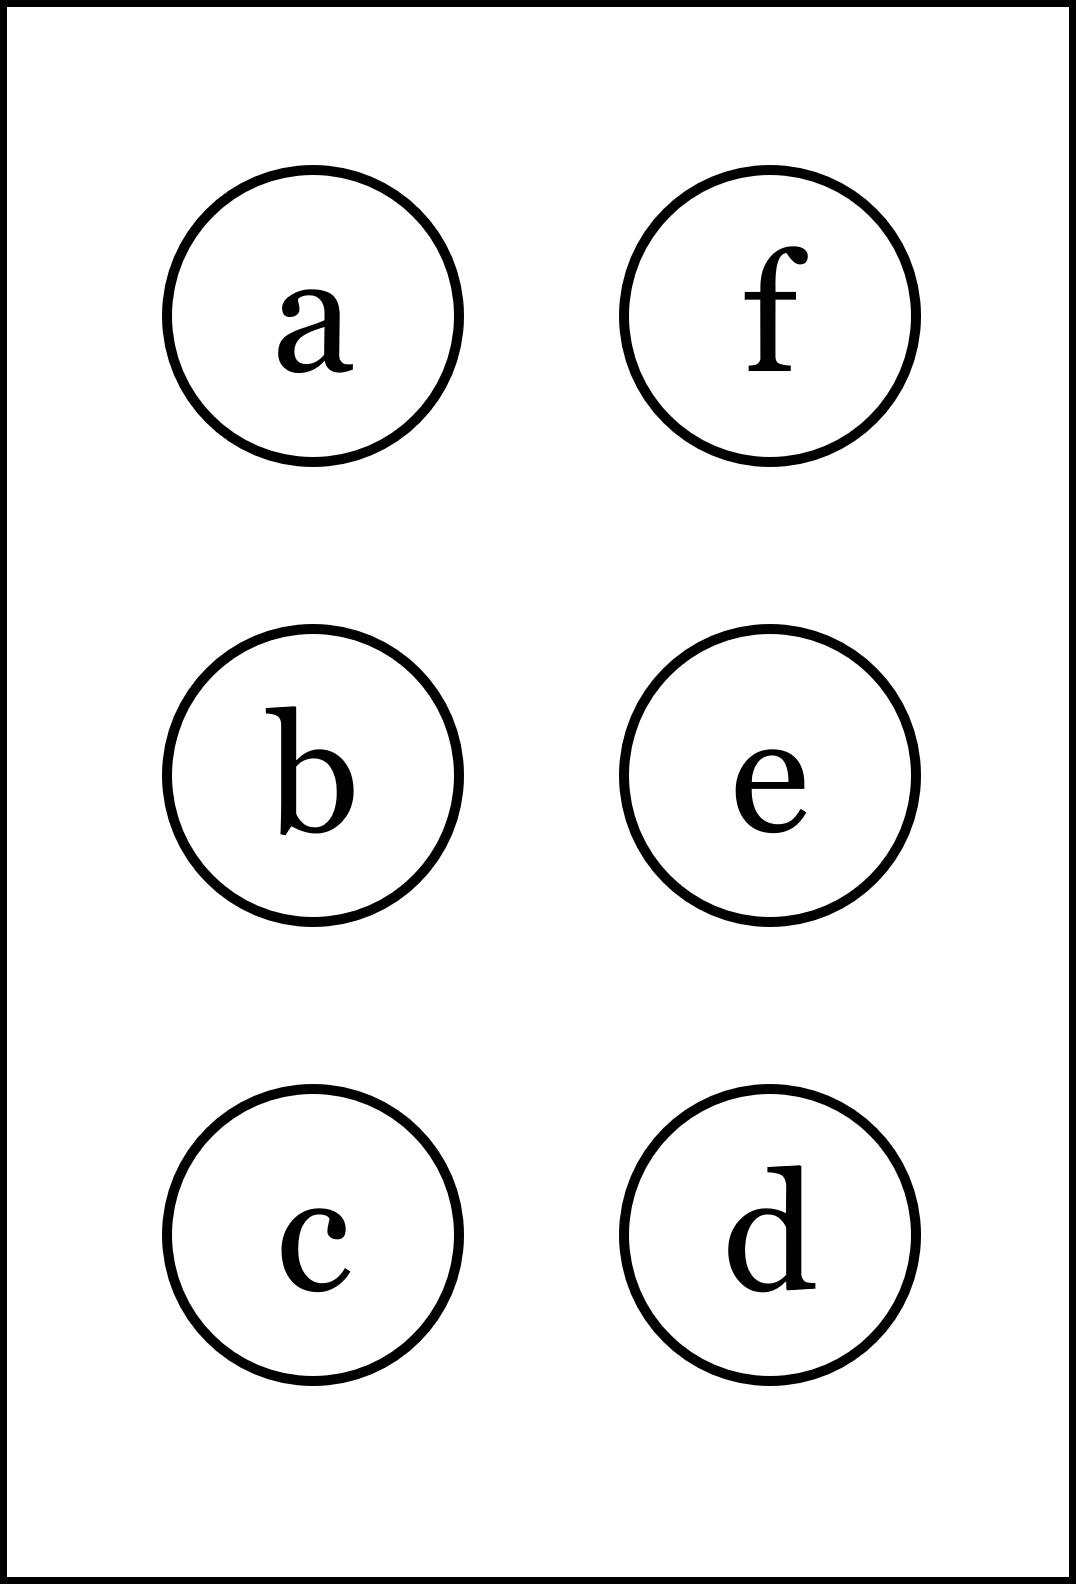
\includegraphics[height=40mm]{../images/braille.png}
{\small Písmeno Braillovej abecedy}
\end{center}
\end{minipage}
\end{center}
\end{minipage}
\\ \hdashline
\begin{minipage}[c][104.5mm][t]{0.5\linewidth}
\begin{center}
\vspace{7mm}
{\huge Kvadratická rovnice, skupina \textit{Epsilon $\epsilon$} -\romannumeral3}\\[5mm]
\textit{Jméno:}\phantom{xxxxxxxxxxxxxxxxxxxxxxxxxxxxxxxxxxxxxxxxxxxxxxxxxxxxxxxxxxxxxxxxx}\\[5mm]
\begin{minipage}{0.95\linewidth}
\begin{center}
V \textbf{(a)} a \textbf{(b)} zjisti počet řešení. V \textbf{(c)} x-ovú polohu vrcholu, a v \textbf{(d)} y-ovú polohu vrcholu.\\V \textbf{(e)} a \textbf{(f)} zjisti součet řešení. Pokud ti vyjde stejný výsledek jako je za otazníky, tak\\napravo obarvi příslušející kroužek načerno. \textbf{Spolu odevzdejte výsledné slovo}.
\end{center}
\end{minipage}
\\[1mm]
\begin{minipage}{0.79\linewidth}
\begin{center}
\begin{varwidth}{\linewidth}
\begin{enumerate}
\Large
\item $-7x^2+5x-7=0$\quad \dotfill\; ???\;\dotfill \quad 0
\item $-6x^2+5x+1=0$\quad \dotfill\; ???\;\dotfill \quad 2
\item $f(x)=-3x^2+2x+5$\quad \dotfill\; ???\;\dotfill \quad $\nicefrac{1}{3}$
\item $f(x)=-8x^2-6x+3$\quad \dotfill\; ???\;\dotfill \quad $\nicefrac{21}{8}$
\item $-x^2-x+2=0$\quad \dotfill\; ???\;\dotfill \quad -1
\item $-16x^2+10x-1=0$\quad \dotfill\; ???\;\dotfill \quad $\nicefrac{3}{8}$
\end{enumerate}
\end{varwidth}
\end{center}
\end{minipage}
\begin{minipage}{0.20\linewidth}
\begin{center}
{\Huge\bfseries 3.} \\[2mm]
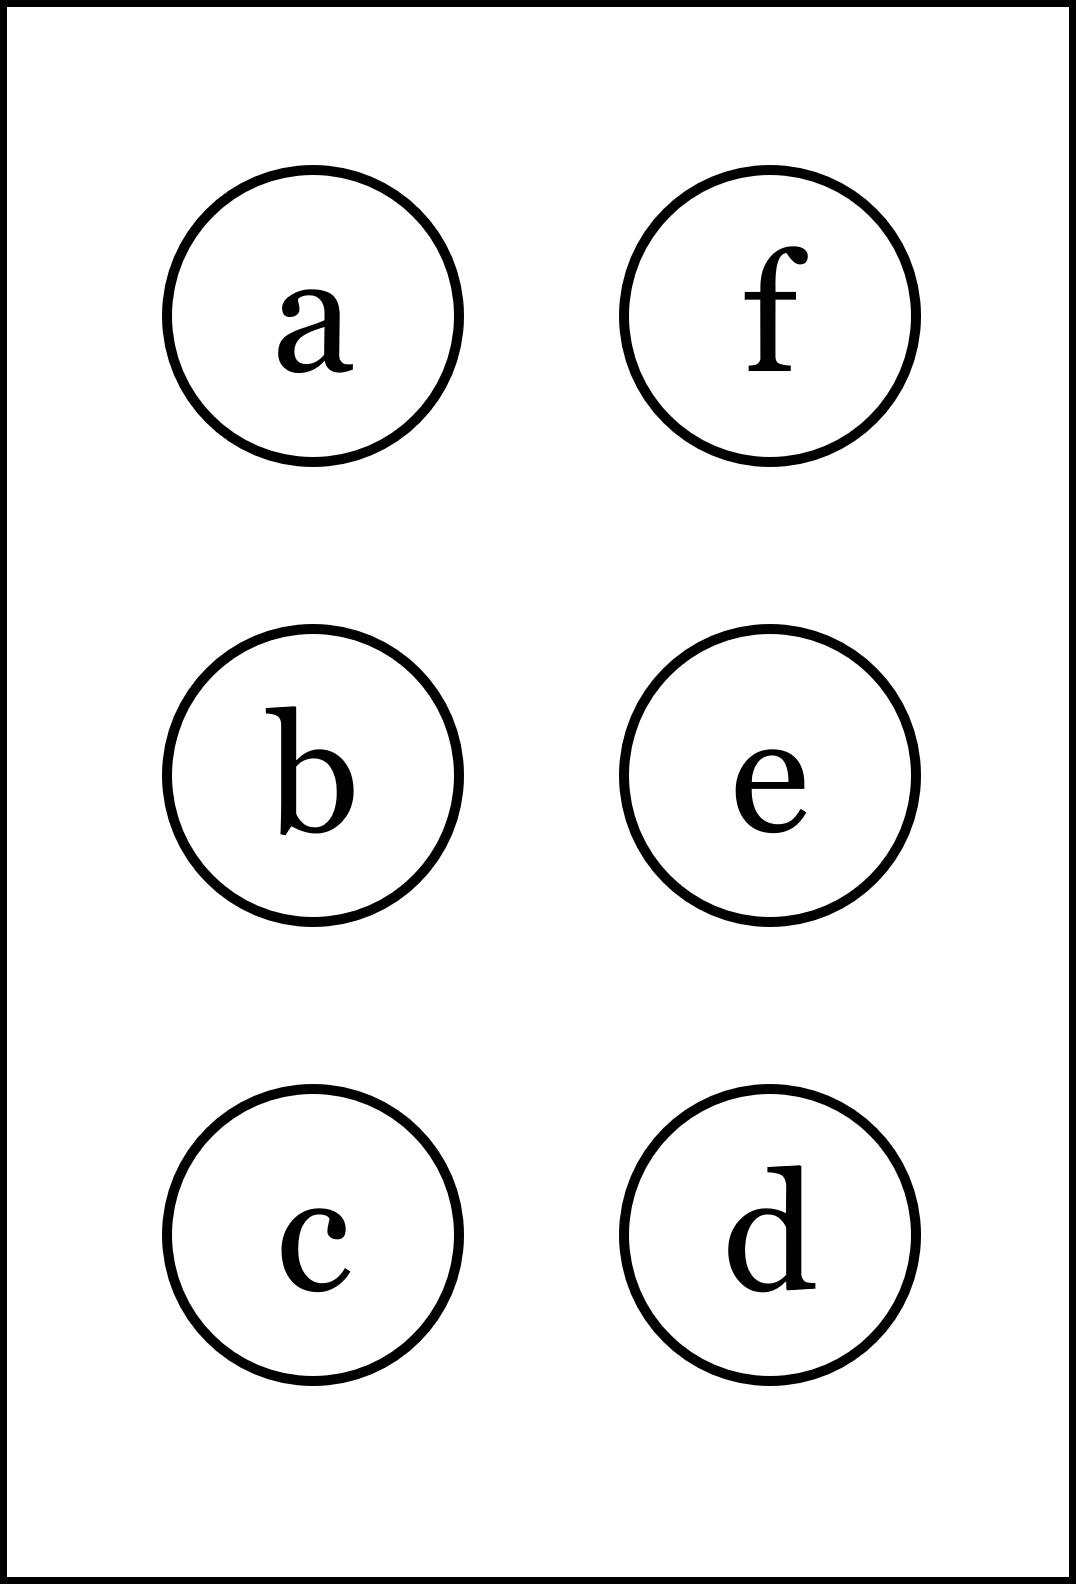
\includegraphics[height=40mm]{../images/braille.png}
{\small Písmeno Braillovej abecedy}
\end{center}
\end{minipage}
\end{center}
\end{minipage}
&
\begin{minipage}[c][104.5mm][t]{0.5\linewidth}
\begin{center}
\vspace{7mm}
{\huge Kvadratická rovnice, skupina \textit{Epsilon $\epsilon$} -\romannumeral4}\\[5mm]
\textit{Jméno:}\phantom{xxxxxxxxxxxxxxxxxxxxxxxxxxxxxxxxxxxxxxxxxxxxxxxxxxxxxxxxxxxxxxxxx}\\[5mm]
\begin{minipage}{0.95\linewidth}
\begin{center}
V \textbf{(a)} a \textbf{(b)} zjisti počet řešení. V \textbf{(c)} x-ovú polohu vrcholu, a v \textbf{(d)} y-ovú polohu vrcholu.\\V \textbf{(e)} a \textbf{(f)} zjisti součet řešení. Pokud ti vyjde stejný výsledek jako je za otazníky, tak\\napravo obarvi příslušející kroužek načerno. \textbf{Spolu odevzdejte výsledné slovo}.
\end{center}
\end{minipage}
\\[1mm]
\begin{minipage}{0.79\linewidth}
\begin{center}
\begin{varwidth}{\linewidth}
\begin{enumerate}
\Large
\item $-3x^2+x-5=0$\quad \dotfill\; ???\;\dotfill \quad 0
\item $5x^2+2x-5=0$\quad \dotfill\; ???\;\dotfill \quad 1
\item $f(x)=5x^2+7x+3$\quad \dotfill\; ???\;\dotfill \quad $\nicefrac{7}{10}$
\item $f(x)=x^2-4x-7$\quad \dotfill\; ???\;\dotfill \quad $\nicefrac{-15}{2}$
\item $3x^2-21x+36=0$\quad \dotfill\; ???\;\dotfill \quad 8
\item $-x^2+x+2=0$\quad \dotfill\; ???\;\dotfill \quad $3$
\end{enumerate}
\end{varwidth}
\end{center}
\end{minipage}
\begin{minipage}{0.20\linewidth}
\begin{center}
{\Huge\bfseries 4.} \\[2mm]
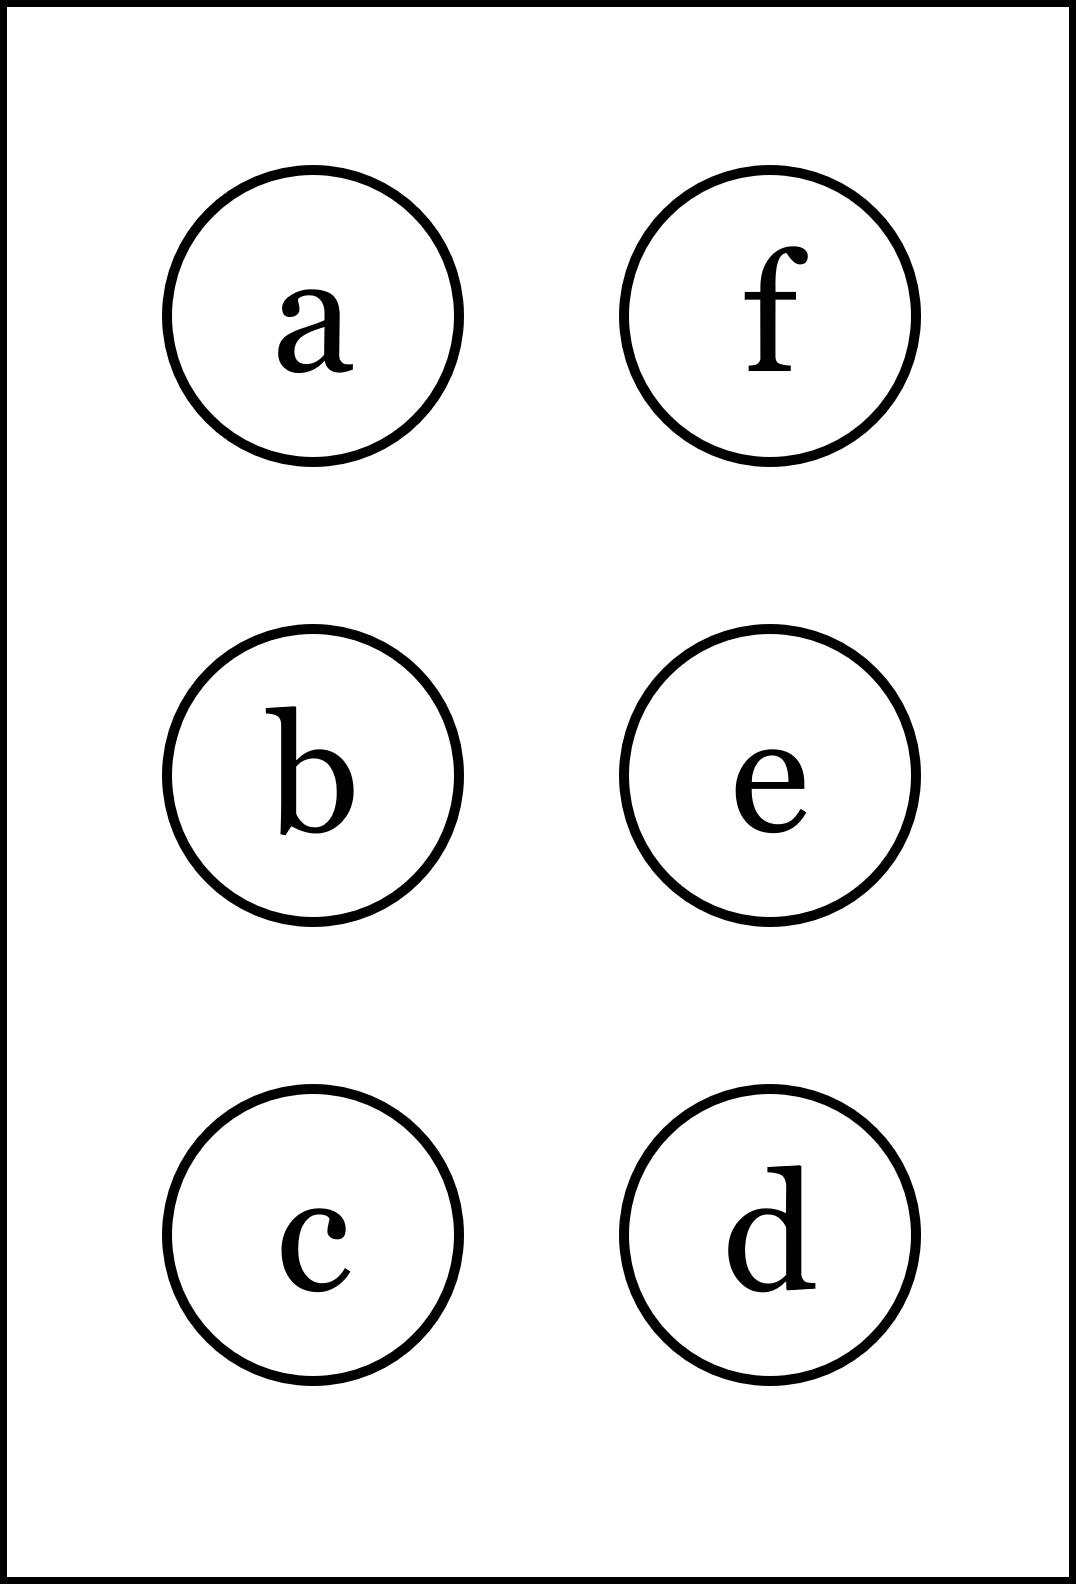
\includegraphics[height=40mm]{../images/braille.png}
{\small Písmeno Braillovej abecedy}
\end{center}
\end{minipage}
\end{center}
\end{minipage}
%
\end{tabular}
\newpage
\thispagestyle{empty}
\begin{tabular}{c:c}
\begin{minipage}[c][104.5mm][t]{0.5\linewidth}
\begin{center}
\vspace{7mm}
{\huge Kvadratická rovnice, skupina \textit{Zeta $\zeta$} -\romannumeral1}\\[5mm]
\textit{Jméno:}\phantom{xxxxxxxxxxxxxxxxxxxxxxxxxxxxxxxxxxxxxxxxxxxxxxxxxxxxxxxxxxxxxxxxx}\\[5mm]
\begin{minipage}{0.95\linewidth}
\begin{center}
V \textbf{(a)} a \textbf{(b)} zjisti počet řešení. V \textbf{(c)} x-ovú polohu vrcholu, a v \textbf{(d)} y-ovú polohu vrcholu.\\V \textbf{(e)} a \textbf{(f)} zjisti součet řešení. Pokud ti vyjde stejný výsledek jako je za otazníky, tak\\napravo obarvi příslušející kroužek načerno. \textbf{Spolu odevzdejte výsledné slovo}.
\end{center}
\end{minipage}
\\[1mm]
\begin{minipage}{0.79\linewidth}
\begin{center}
\begin{varwidth}{\linewidth}
\begin{enumerate}
\Large
\item $-x^2+x-1=0$\quad \dotfill\; ???\;\dotfill \quad 0
\item $-3x^2-5x+1=0$\quad \dotfill\; ???\;\dotfill \quad 1
\item $f(x)=5x^2+8x-1$\quad \dotfill\; ???\;\dotfill \quad $\nicefrac{-4}{5}$
\item $f(x)=-6x^2-x-5$\quad \dotfill\; ???\;\dotfill \quad $\nicefrac{-119}{24}$
\item $3x^2-18x+15=0$\quad \dotfill\; ???\;\dotfill \quad 6
\item $2x^2+11x+5=0$\quad \dotfill\; ???\;\dotfill \quad $\nicefrac{-9}{2}$
\end{enumerate}
\end{varwidth}
\end{center}
\end{minipage}
\begin{minipage}{0.20\linewidth}
\begin{center}
{\Huge\bfseries 1.} \\[2mm]
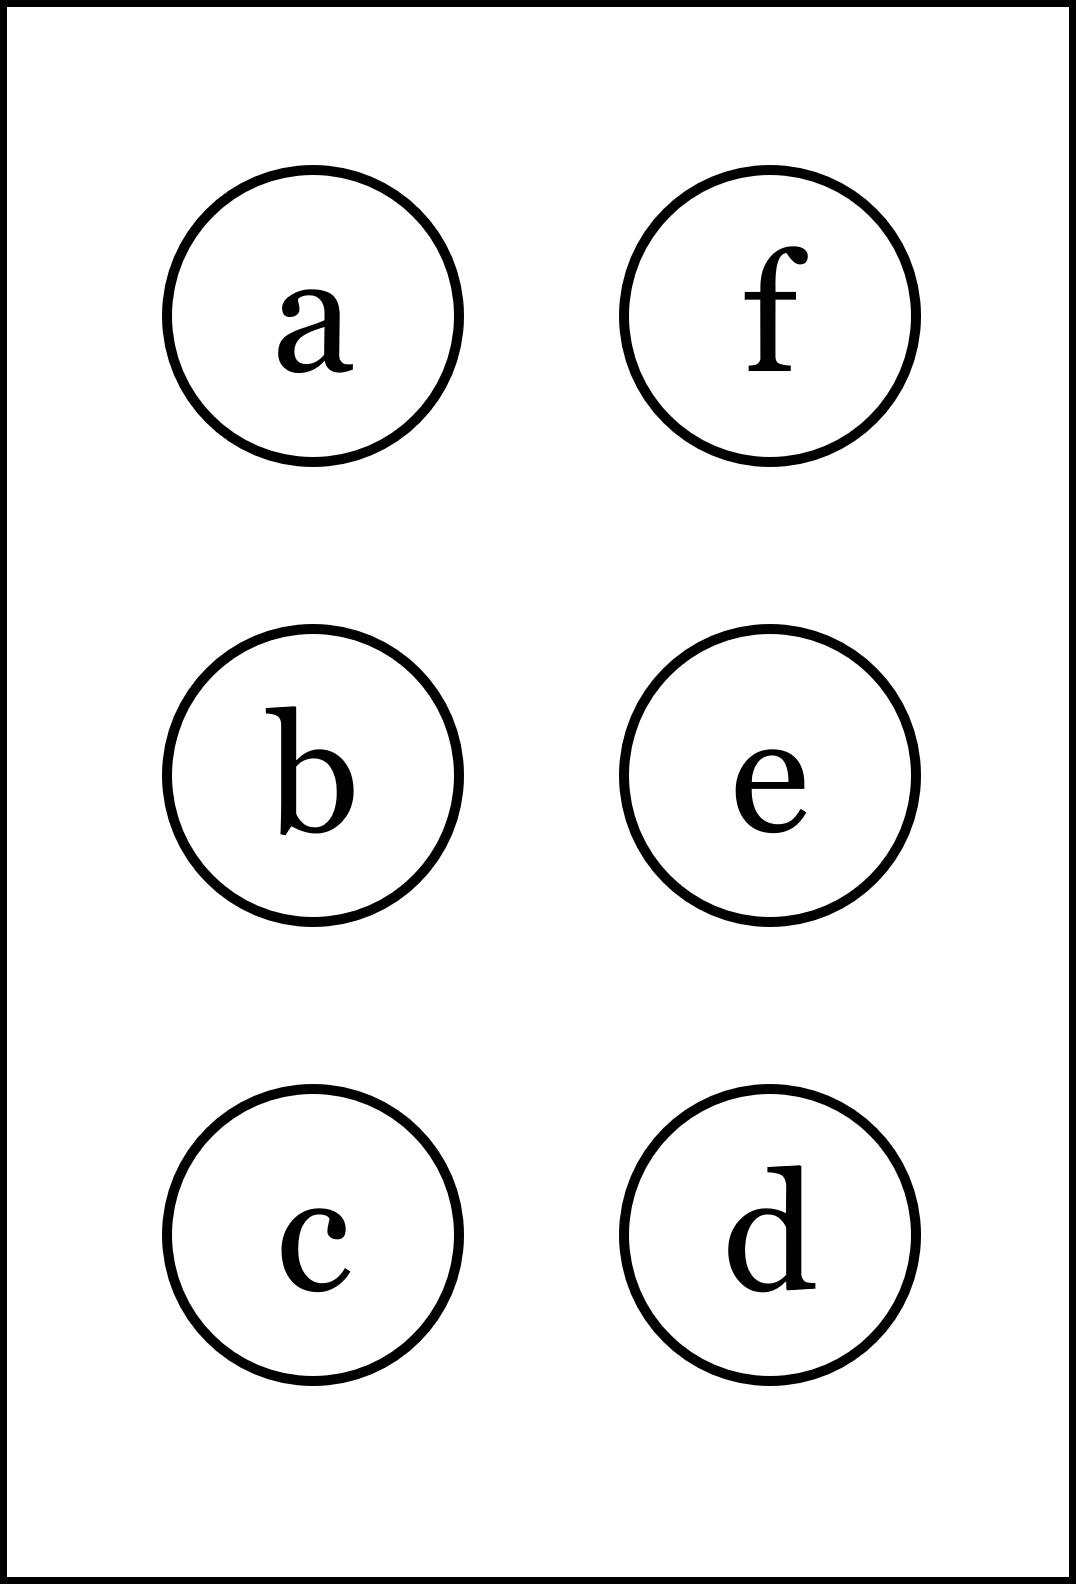
\includegraphics[height=40mm]{../images/braille.png}
{\small Písmeno Braillovej abecedy}
\end{center}
\end{minipage}
\end{center}
\end{minipage}
&
\begin{minipage}[c][104.5mm][t]{0.5\linewidth}
\begin{center}
\vspace{7mm}
{\huge Kvadratická rovnice, skupina \textit{Zeta $\zeta$} -\romannumeral2}\\[5mm]
\textit{Jméno:}\phantom{xxxxxxxxxxxxxxxxxxxxxxxxxxxxxxxxxxxxxxxxxxxxxxxxxxxxxxxxxxxxxxxxx}\\[5mm]
\begin{minipage}{0.95\linewidth}
\begin{center}
V \textbf{(a)} a \textbf{(b)} zjisti počet řešení. V \textbf{(c)} x-ovú polohu vrcholu, a v \textbf{(d)} y-ovú polohu vrcholu.\\V \textbf{(e)} a \textbf{(f)} zjisti součet řešení. Pokud ti vyjde stejný výsledek jako je za otazníky, tak\\napravo obarvi příslušející kroužek načerno. \textbf{Spolu odevzdejte výsledné slovo}.
\end{center}
\end{minipage}
\\[1mm]
\begin{minipage}{0.79\linewidth}
\begin{center}
\begin{varwidth}{\linewidth}
\begin{enumerate}
\Large
\item $2x^2+7x-4=0$\quad \dotfill\; ???\;\dotfill \quad 2
\item $-8x^2-3x-3=0$\quad \dotfill\; ???\;\dotfill \quad 2
\item $f(x)=-2x^2-x-1$\quad \dotfill\; ???\;\dotfill \quad $\nicefrac{-1}{4}$
\item $f(x)=-7x^2-3x+3$\quad \dotfill\; ???\;\dotfill \quad $\nicefrac{93}{28}$
\item $-2x^2-10x+12=0$\quad \dotfill\; ???\;\dotfill \quad -3
\item $9x^2+12x+3=0$\quad \dotfill\; ???\;\dotfill \quad $\nicefrac{2}{3}$
\end{enumerate}
\end{varwidth}
\end{center}
\end{minipage}
\begin{minipage}{0.20\linewidth}
\begin{center}
{\Huge\bfseries 2.} \\[2mm]
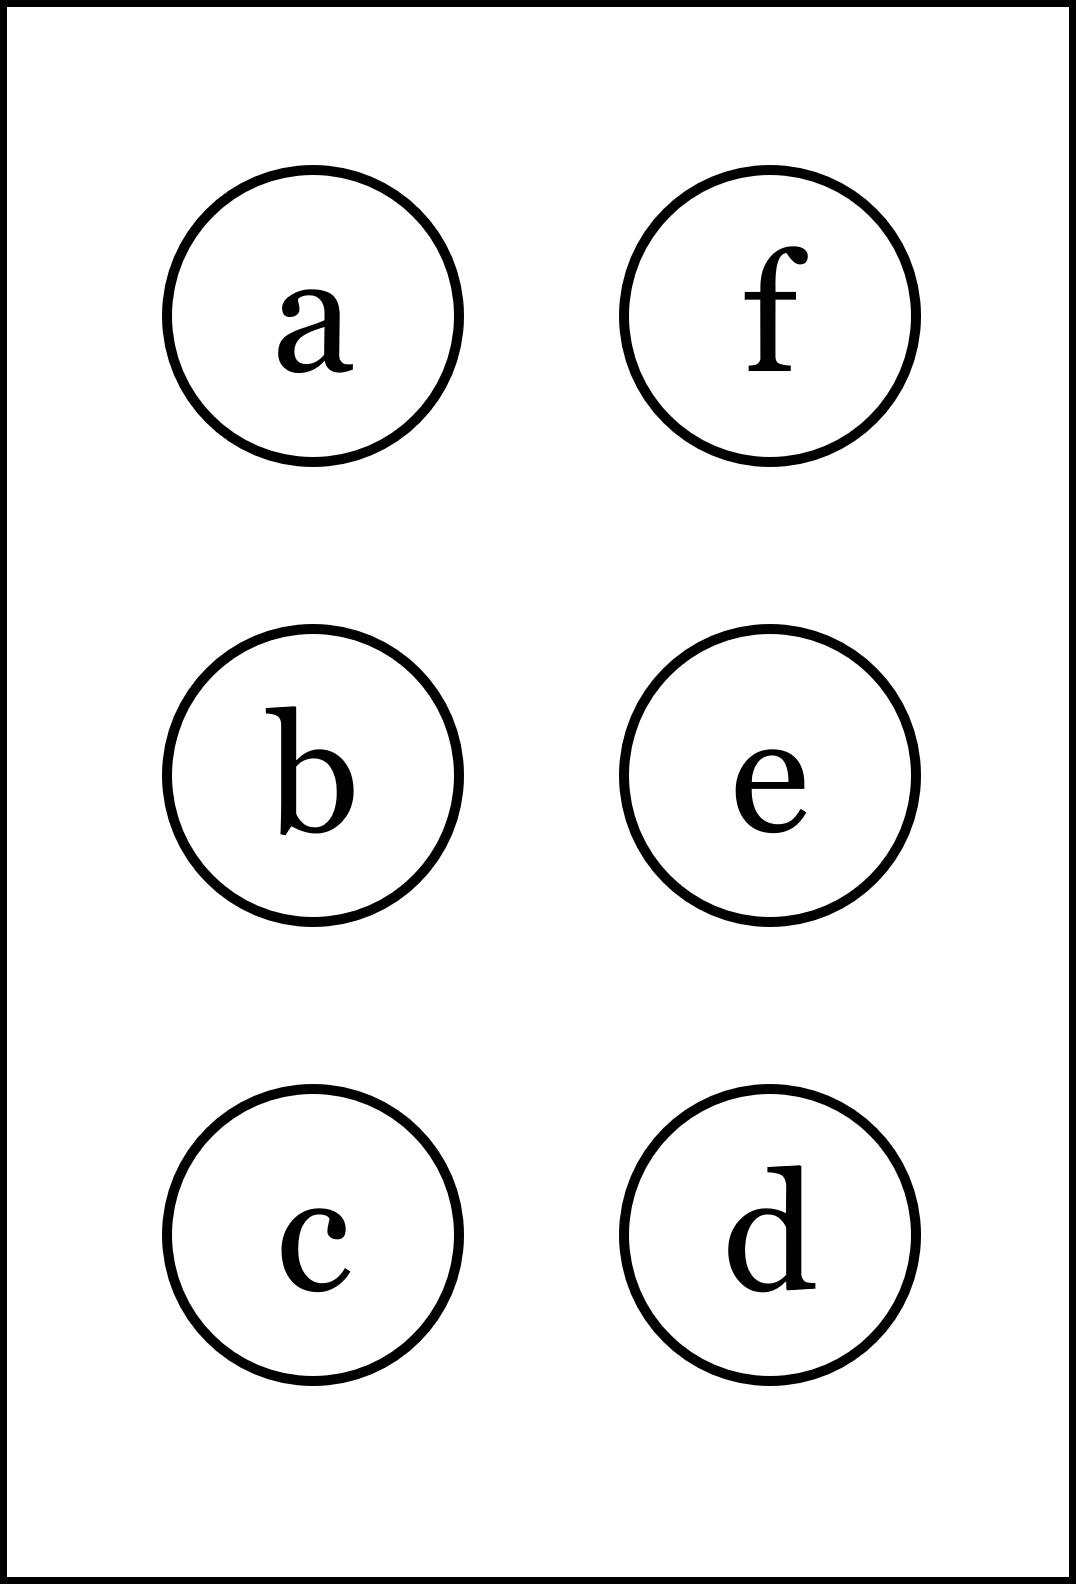
\includegraphics[height=40mm]{../images/braille.png}
{\small Písmeno Braillovej abecedy}
\end{center}
\end{minipage}
\end{center}
\end{minipage}
\\ \hdashline
\begin{minipage}[c][104.5mm][t]{0.5\linewidth}
\begin{center}
\vspace{7mm}
{\huge Kvadratická rovnice, skupina \textit{Zeta $\zeta$} -\romannumeral3}\\[5mm]
\textit{Jméno:}\phantom{xxxxxxxxxxxxxxxxxxxxxxxxxxxxxxxxxxxxxxxxxxxxxxxxxxxxxxxxxxxxxxxxx}\\[5mm]
\begin{minipage}{0.95\linewidth}
\begin{center}
V \textbf{(a)} a \textbf{(b)} zjisti počet řešení. V \textbf{(c)} x-ovú polohu vrcholu, a v \textbf{(d)} y-ovú polohu vrcholu.\\V \textbf{(e)} a \textbf{(f)} zjisti součet řešení. Pokud ti vyjde stejný výsledek jako je za otazníky, tak\\napravo obarvi příslušející kroužek načerno. \textbf{Spolu odevzdejte výsledné slovo}.
\end{center}
\end{minipage}
\\[1mm]
\begin{minipage}{0.79\linewidth}
\begin{center}
\begin{varwidth}{\linewidth}
\begin{enumerate}
\Large
\item $-2x^2+5x+3=0$\quad \dotfill\; ???\;\dotfill \quad 2
\item $-4x^2-4x-6=0$\quad \dotfill\; ???\;\dotfill \quad 0
\item $f(x)=3x^2+8x-1$\quad \dotfill\; ???\;\dotfill \quad $\nicefrac{4}{3}$
\item $f(x)=2x^2-x+7$\quad \dotfill\; ???\;\dotfill \quad $\nicefrac{27}{8}$
\item $x^2+x-2=0$\quad \dotfill\; ???\;\dotfill \quad 1
\item $-5x^2-15x-10=0$\quad \dotfill\; ???\;\dotfill \quad $1$
\end{enumerate}
\end{varwidth}
\end{center}
\end{minipage}
\begin{minipage}{0.20\linewidth}
\begin{center}
{\Huge\bfseries 3.} \\[2mm]
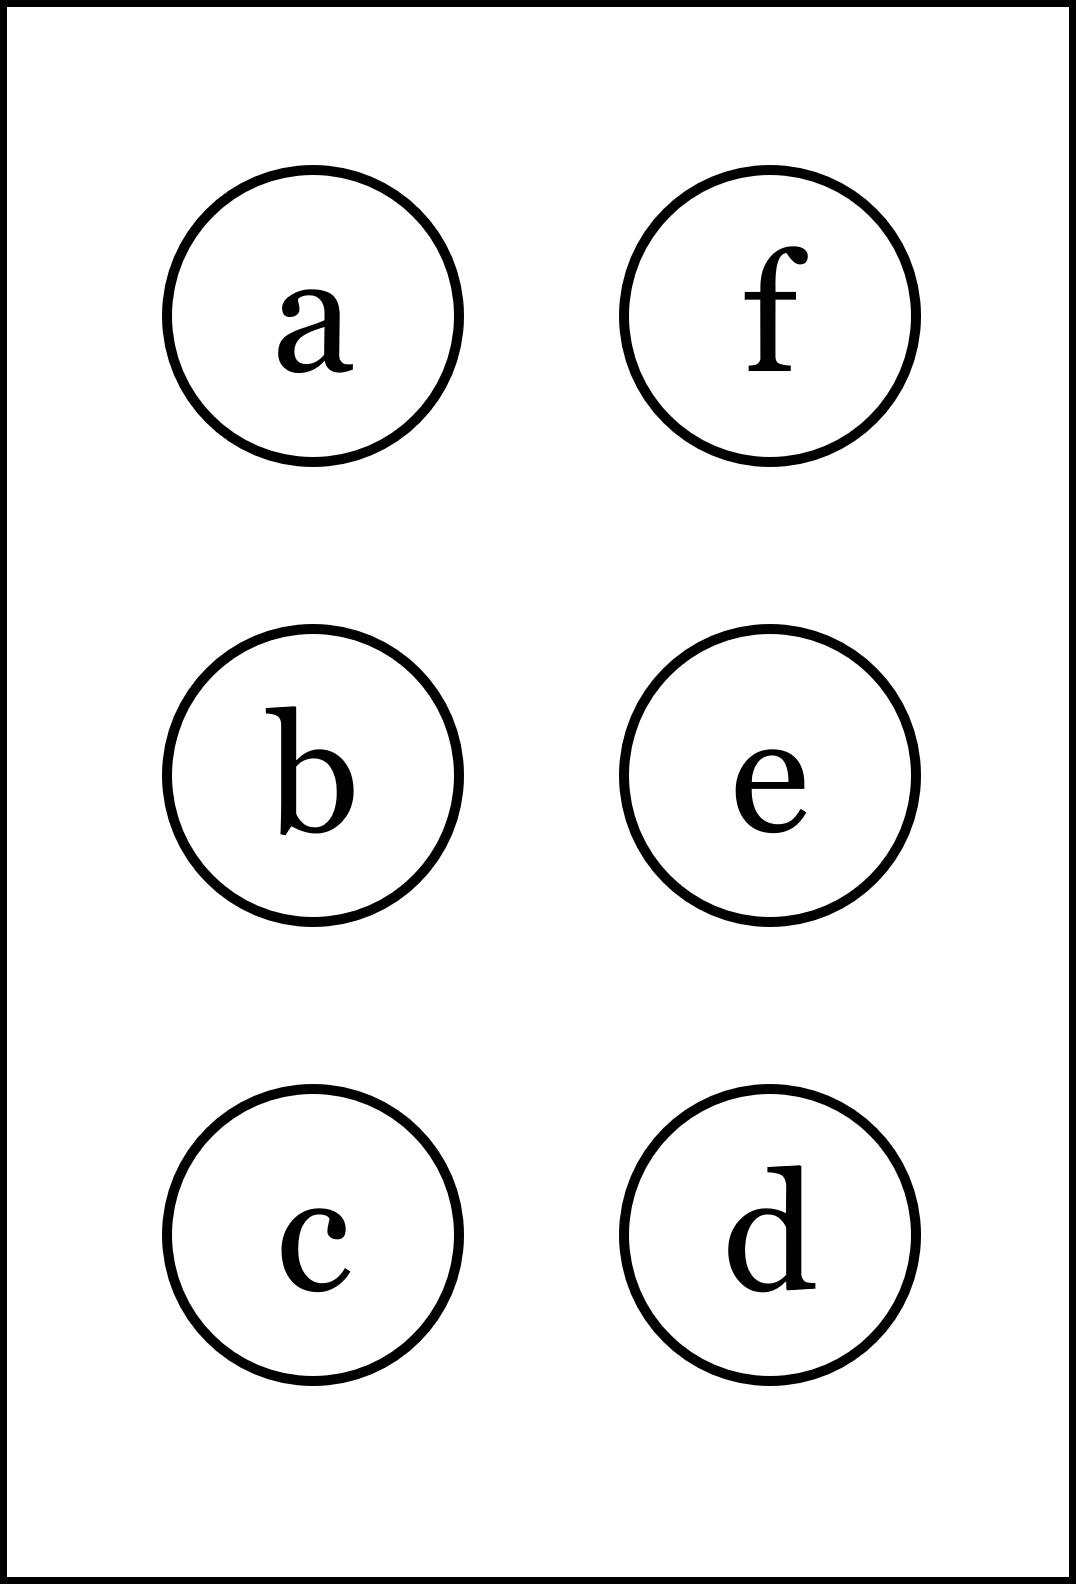
\includegraphics[height=40mm]{../images/braille.png}
{\small Písmeno Braillovej abecedy}
\end{center}
\end{minipage}
\end{center}
\end{minipage}
&
\begin{minipage}[c][104.5mm][t]{0.5\linewidth}
\begin{center}
\vspace{7mm}
{\huge Kvadratická rovnice, skupina \textit{Zeta $\zeta$} -\romannumeral4}\\[5mm]
\textit{Jméno:}\phantom{xxxxxxxxxxxxxxxxxxxxxxxxxxxxxxxxxxxxxxxxxxxxxxxxxxxxxxxxxxxxxxxxx}\\[5mm]
\begin{minipage}{0.95\linewidth}
\begin{center}
V \textbf{(a)} a \textbf{(b)} zjisti počet řešení. V \textbf{(c)} x-ovú polohu vrcholu, a v \textbf{(d)} y-ovú polohu vrcholu.\\V \textbf{(e)} a \textbf{(f)} zjisti součet řešení. Pokud ti vyjde stejný výsledek jako je za otazníky, tak\\napravo obarvi příslušející kroužek načerno. \textbf{Spolu odevzdejte výsledné slovo}.
\end{center}
\end{minipage}
\\[1mm]
\begin{minipage}{0.79\linewidth}
\begin{center}
\begin{varwidth}{\linewidth}
\begin{enumerate}
\Large
\item $-5x^2+9x+6=0$\quad \dotfill\; ???\;\dotfill \quad 2
\item $-3x^2-x+3=0$\quad \dotfill\; ???\;\dotfill \quad 1
\item $f(x)=4x^2+x+1$\quad \dotfill\; ???\;\dotfill \quad $\nicefrac{-1}{8}$
\item $f(x)=-2x^2-5x+2$\quad \dotfill\; ???\;\dotfill \quad $\nicefrac{41}{8}$
\item $-2x^2-10x-12=0$\quad \dotfill\; ???\;\dotfill \quad -5
\item $-x^2-8x-7=0$\quad \dotfill\; ???\;\dotfill \quad $-8$
\end{enumerate}
\end{varwidth}
\end{center}
\end{minipage}
\begin{minipage}{0.20\linewidth}
\begin{center}
{\Huge\bfseries 4.} \\[2mm]
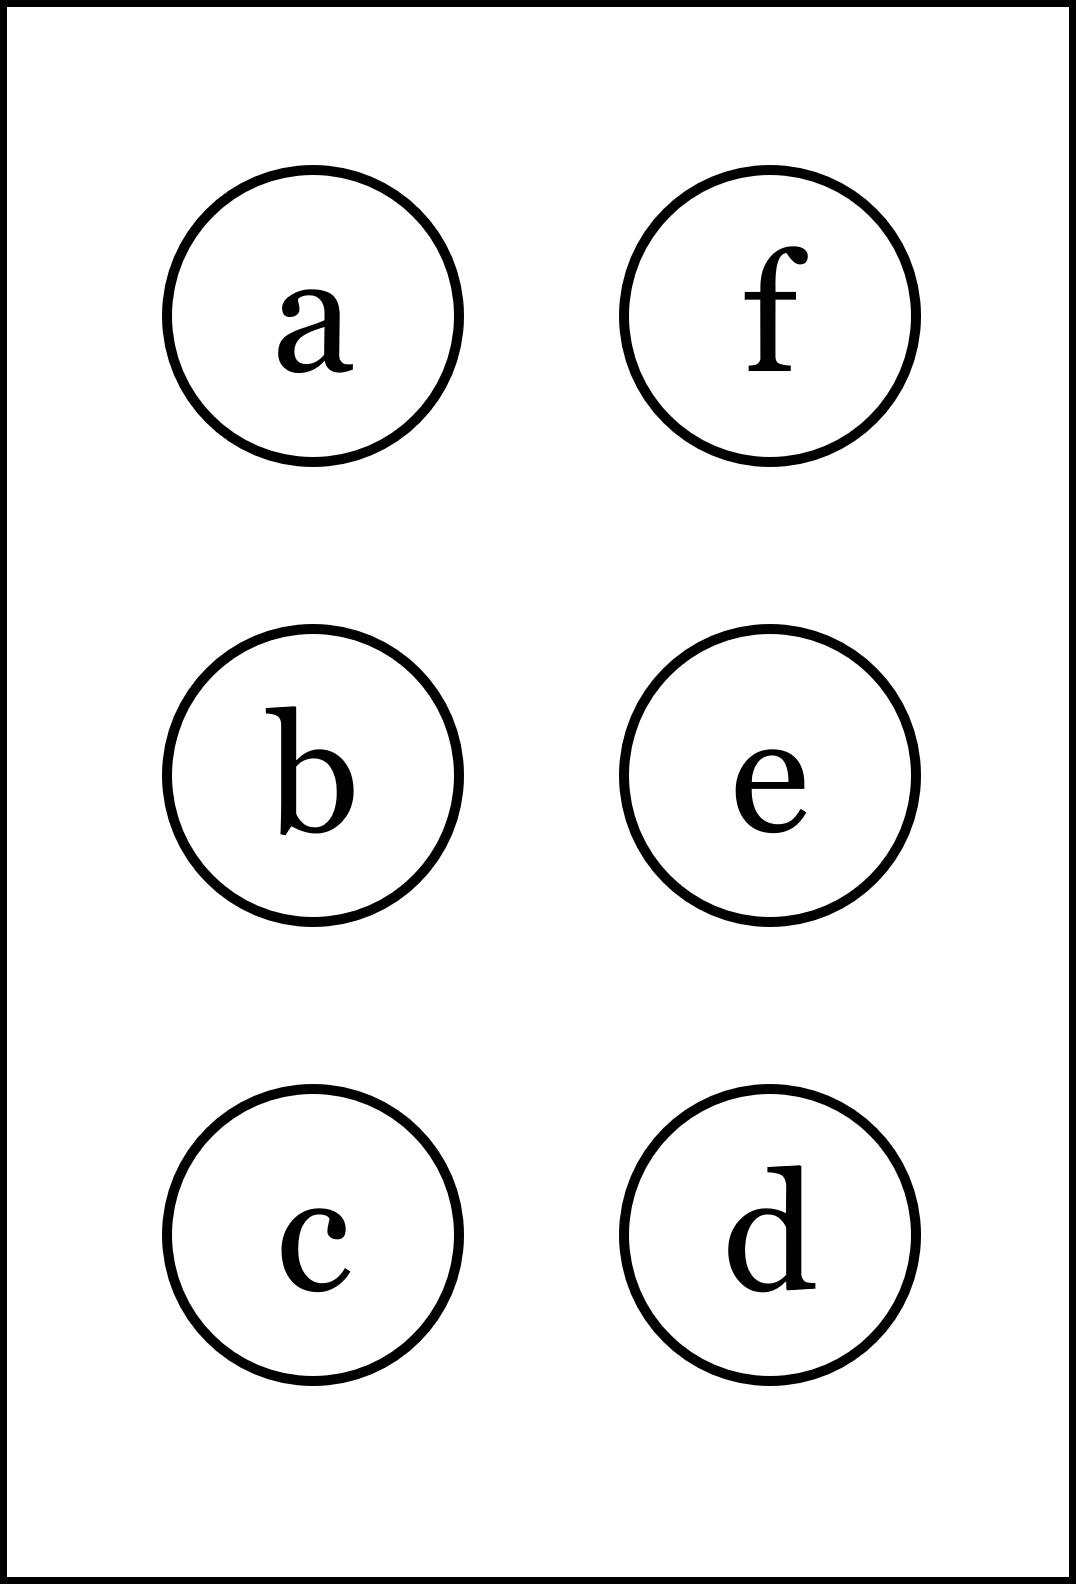
\includegraphics[height=40mm]{../images/braille.png}
{\small Písmeno Braillovej abecedy}
\end{center}
\end{minipage}
\end{center}
\end{minipage}
%
\end{tabular}
\newpage
\thispagestyle{empty}
\begin{tabular}{c:c}
\begin{minipage}[c][104.5mm][t]{0.5\linewidth}
\begin{center}
\vspace{7mm}
{\huge Kvadratická rovnice, skupina \textit{Eta $\eta$} -\romannumeral1}\\[5mm]
\textit{Jméno:}\phantom{xxxxxxxxxxxxxxxxxxxxxxxxxxxxxxxxxxxxxxxxxxxxxxxxxxxxxxxxxxxxxxxxx}\\[5mm]
\begin{minipage}{0.95\linewidth}
\begin{center}
V \textbf{(a)} a \textbf{(b)} zjisti počet řešení. V \textbf{(c)} x-ovú polohu vrcholu, a v \textbf{(d)} y-ovú polohu vrcholu.\\V \textbf{(e)} a \textbf{(f)} zjisti součet řešení. Pokud ti vyjde stejný výsledek jako je za otazníky, tak\\napravo obarvi příslušející kroužek načerno. \textbf{Spolu odevzdejte výsledné slovo}.
\end{center}
\end{minipage}
\\[1mm]
\begin{minipage}{0.79\linewidth}
\begin{center}
\begin{varwidth}{\linewidth}
\begin{enumerate}
\Large
\item $-6x^2+3x+1=0$\quad \dotfill\; ???\;\dotfill \quad 2
\item $2x^2+2x+3=0$\quad \dotfill\; ???\;\dotfill \quad 1
\item $f(x)=-3x^2+x+5$\quad \dotfill\; ???\;\dotfill \quad $\nicefrac{1}{6}$
\item $f(x)=-9x^2+6x-2$\quad \dotfill\; ???\;\dotfill \quad $0$
\item $-x^2-11x-24=0$\quad \dotfill\; ???\;\dotfill \quad -13
\item $-9x^2+6x+3=0$\quad \dotfill\; ???\;\dotfill \quad $\nicefrac{4}{3}$
\end{enumerate}
\end{varwidth}
\end{center}
\end{minipage}
\begin{minipage}{0.20\linewidth}
\begin{center}
{\Huge\bfseries 1.} \\[2mm]
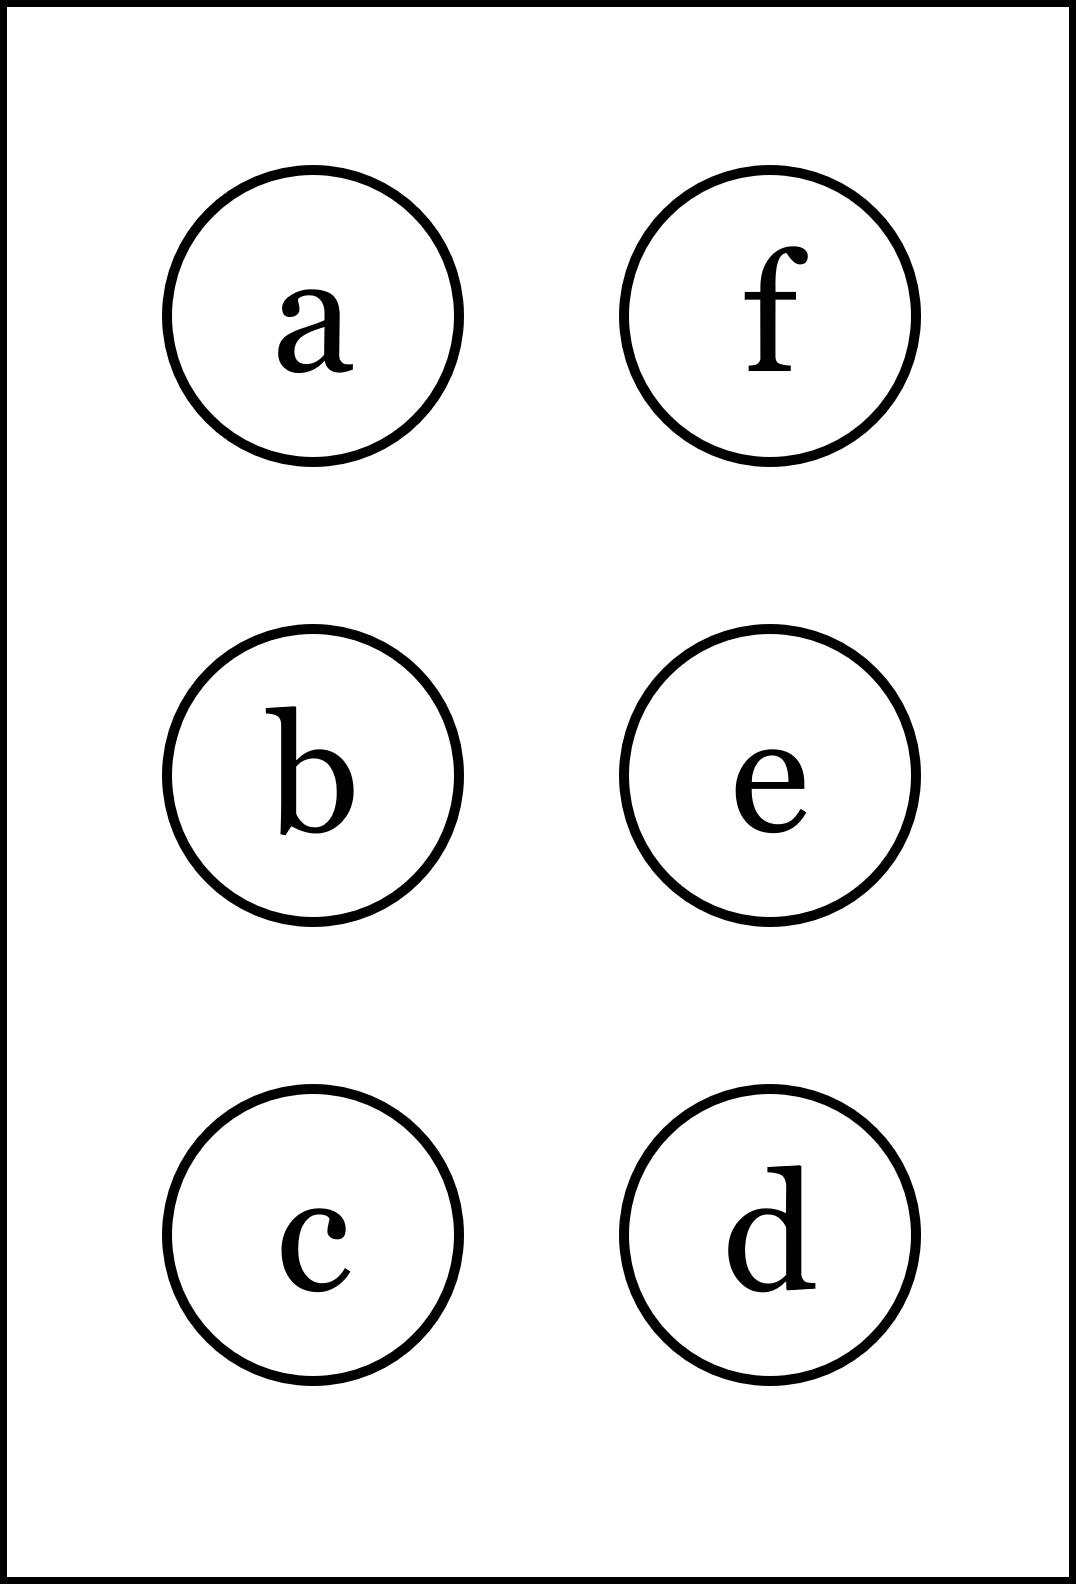
\includegraphics[height=40mm]{../images/braille.png}
{\small Písmeno Braillovej abecedy}
\end{center}
\end{minipage}
\end{center}
\end{minipage}
&
\begin{minipage}[c][104.5mm][t]{0.5\linewidth}
\begin{center}
\vspace{7mm}
{\huge Kvadratická rovnice, skupina \textit{Eta $\eta$} -\romannumeral2}\\[5mm]
\textit{Jméno:}\phantom{xxxxxxxxxxxxxxxxxxxxxxxxxxxxxxxxxxxxxxxxxxxxxxxxxxxxxxxxxxxxxxxxx}\\[5mm]
\begin{minipage}{0.95\linewidth}
\begin{center}
V \textbf{(a)} a \textbf{(b)} zjisti počet řešení. V \textbf{(c)} x-ovú polohu vrcholu, a v \textbf{(d)} y-ovú polohu vrcholu.\\V \textbf{(e)} a \textbf{(f)} zjisti součet řešení. Pokud ti vyjde stejný výsledek jako je za otazníky, tak\\napravo obarvi příslušející kroužek načerno. \textbf{Spolu odevzdejte výsledné slovo}.
\end{center}
\end{minipage}
\\[1mm]
\begin{minipage}{0.79\linewidth}
\begin{center}
\begin{varwidth}{\linewidth}
\begin{enumerate}
\Large
\item $-2x^2-3x-5=0$\quad \dotfill\; ???\;\dotfill \quad 0
\item $5x^2+4x+3=0$\quad \dotfill\; ???\;\dotfill \quad 1
\item $f(x)=2x^2-2x-8$\quad \dotfill\; ???\;\dotfill \quad $\nicefrac{1}{2}$
\item $f(x)=6x^2+x-4$\quad \dotfill\; ???\;\dotfill \quad $\nicefrac{-49}{24}$
\item $-x^2-9x-14=0$\quad \dotfill\; ???\;\dotfill \quad -9
\item $-10x^2+14x-4=0$\quad \dotfill\; ???\;\dotfill \quad $\nicefrac{-3}{5}$
\end{enumerate}
\end{varwidth}
\end{center}
\end{minipage}
\begin{minipage}{0.20\linewidth}
\begin{center}
{\Huge\bfseries 2.} \\[2mm]
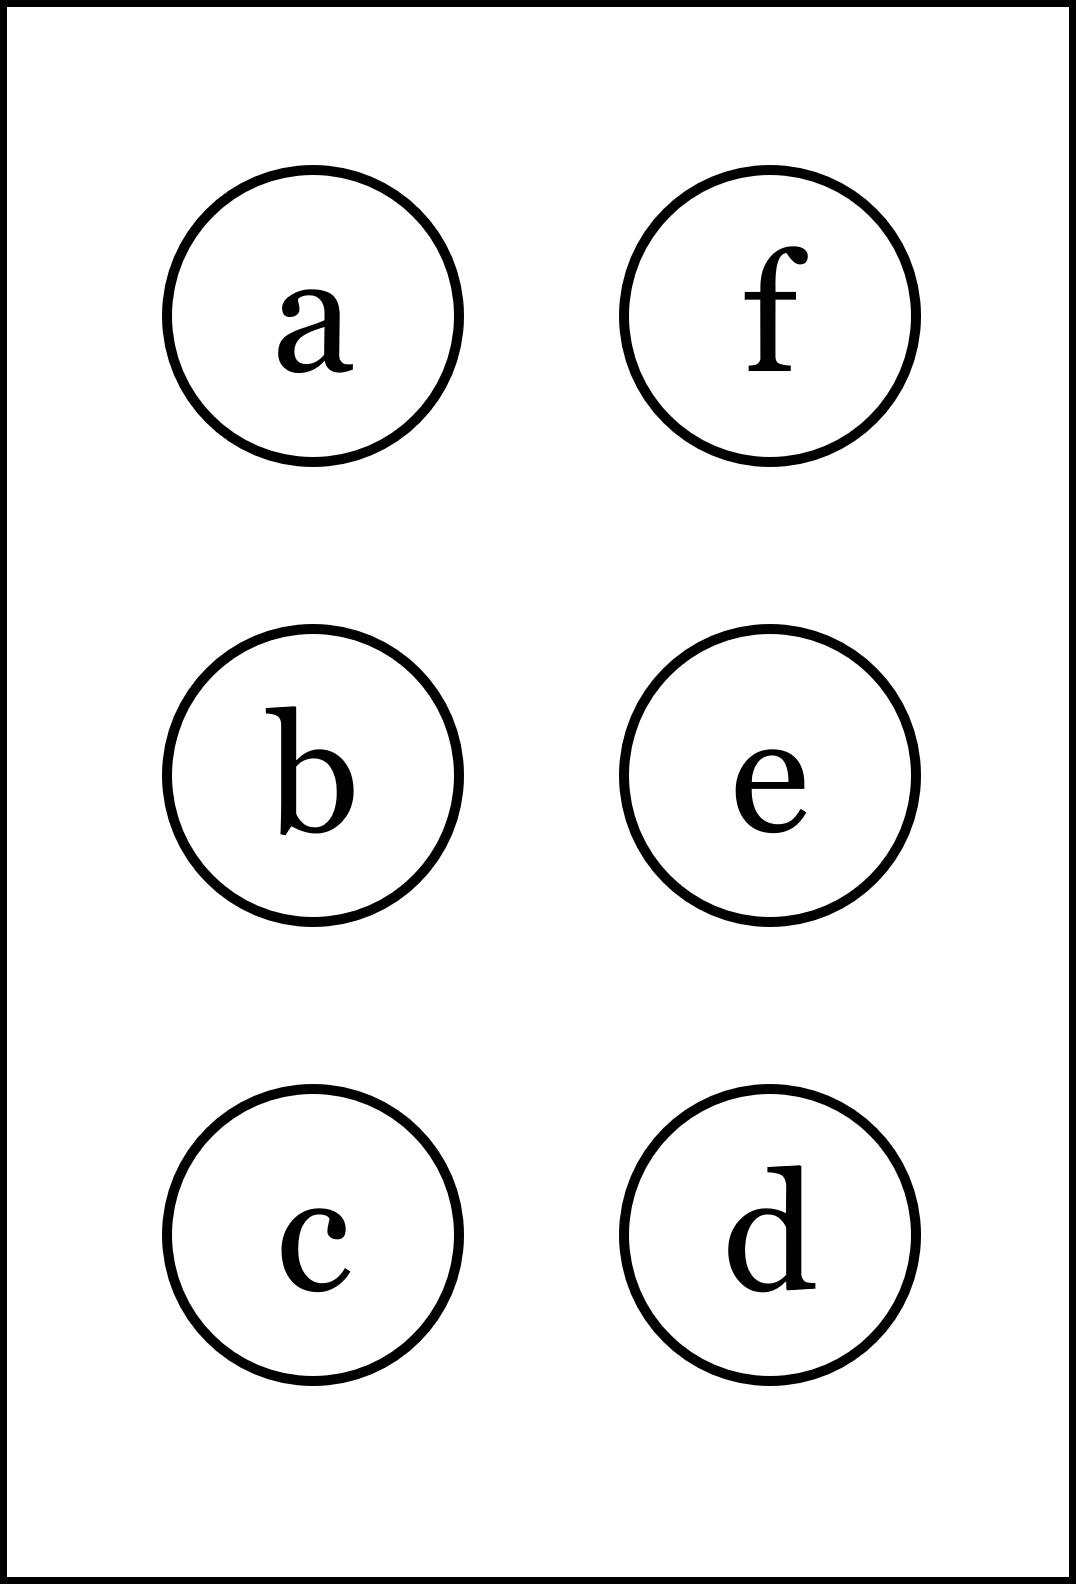
\includegraphics[height=40mm]{../images/braille.png}
{\small Písmeno Braillovej abecedy}
\end{center}
\end{minipage}
\end{center}
\end{minipage}
\\ \hdashline
\begin{minipage}[c][104.5mm][t]{0.5\linewidth}
\begin{center}
\vspace{7mm}
{\huge Kvadratická rovnice, skupina \textit{Eta $\eta$} -\romannumeral3}\\[5mm]
\textit{Jméno:}\phantom{xxxxxxxxxxxxxxxxxxxxxxxxxxxxxxxxxxxxxxxxxxxxxxxxxxxxxxxxxxxxxxxxx}\\[5mm]
\begin{minipage}{0.95\linewidth}
\begin{center}
V \textbf{(a)} a \textbf{(b)} zjisti počet řešení. V \textbf{(c)} x-ovú polohu vrcholu, a v \textbf{(d)} y-ovú polohu vrcholu.\\V \textbf{(e)} a \textbf{(f)} zjisti součet řešení. Pokud ti vyjde stejný výsledek jako je za otazníky, tak\\napravo obarvi příslušející kroužek načerno. \textbf{Spolu odevzdejte výsledné slovo}.
\end{center}
\end{minipage}
\\[1mm]
\begin{minipage}{0.79\linewidth}
\begin{center}
\begin{varwidth}{\linewidth}
\begin{enumerate}
\Large
\item $9x^2+2x+1=0$\quad \dotfill\; ???\;\dotfill \quad 0
\item $-8x^2-4x-3=0$\quad \dotfill\; ???\;\dotfill \quad 0
\item $f(x)=8x^2+2x+6$\quad \dotfill\; ???\;\dotfill \quad $\nicefrac{-1}{8}$
\item $f(x)=2x^2-3x-6$\quad \dotfill\; ???\;\dotfill \quad $\nicefrac{-33}{8}$
\item $6x^2-18x+12=0$\quad \dotfill\; ???\;\dotfill \quad 1
\item $2x^2-x-28=0$\quad \dotfill\; ???\;\dotfill \quad $\nicefrac{-15}{2}$
\end{enumerate}
\end{varwidth}
\end{center}
\end{minipage}
\begin{minipage}{0.20\linewidth}
\begin{center}
{\Huge\bfseries 3.} \\[2mm]
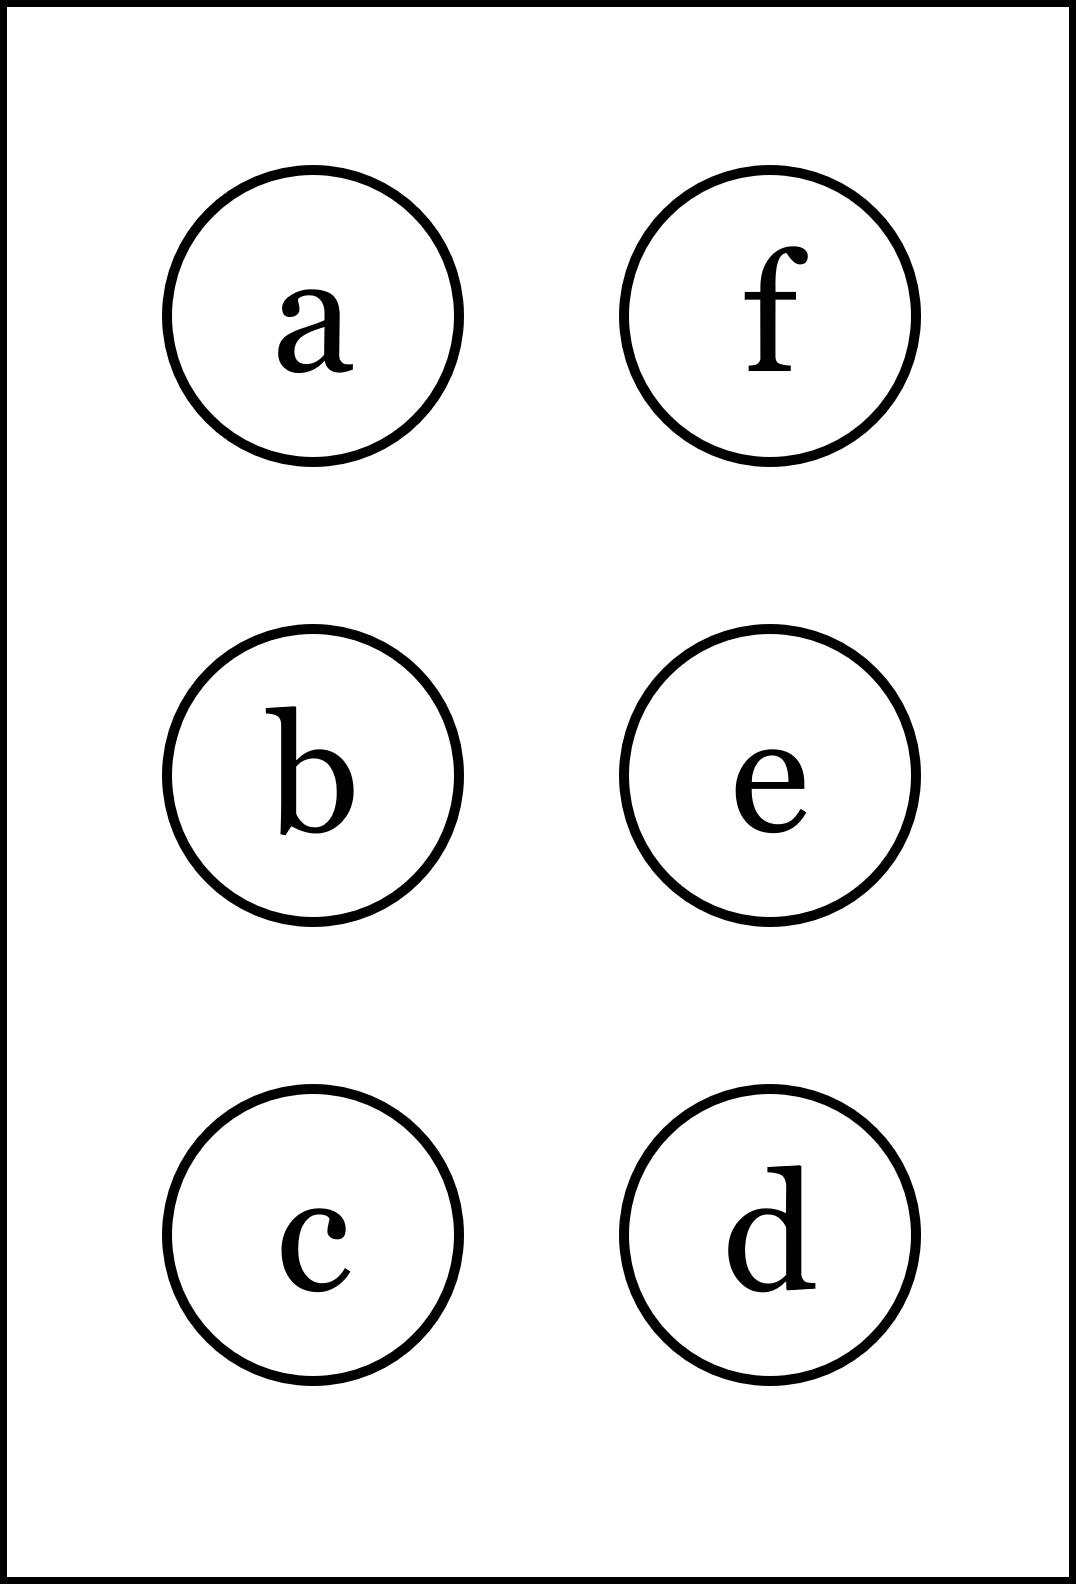
\includegraphics[height=40mm]{../images/braille.png}
{\small Písmeno Braillovej abecedy}
\end{center}
\end{minipage}
\end{center}
\end{minipage}
&
\begin{minipage}[c][104.5mm][t]{0.5\linewidth}
\begin{center}
\vspace{7mm}
{\huge Kvadratická rovnice, skupina \textit{Eta $\eta$} -\romannumeral4}\\[5mm]
\textit{Jméno:}\phantom{xxxxxxxxxxxxxxxxxxxxxxxxxxxxxxxxxxxxxxxxxxxxxxxxxxxxxxxxxxxxxxxxx}\\[5mm]
\begin{minipage}{0.95\linewidth}
\begin{center}
V \textbf{(a)} a \textbf{(b)} zjisti počet řešení. V \textbf{(c)} x-ovú polohu vrcholu, a v \textbf{(d)} y-ovú polohu vrcholu.\\V \textbf{(e)} a \textbf{(f)} zjisti součet řešení. Pokud ti vyjde stejný výsledek jako je za otazníky, tak\\napravo obarvi příslušející kroužek načerno. \textbf{Spolu odevzdejte výsledné slovo}.
\end{center}
\end{minipage}
\\[1mm]
\begin{minipage}{0.79\linewidth}
\begin{center}
\begin{varwidth}{\linewidth}
\begin{enumerate}
\Large
\item $-9x^2+4x-3=0$\quad \dotfill\; ???\;\dotfill \quad 0
\item $-6x^2-5x+7=0$\quad \dotfill\; ???\;\dotfill \quad 0
\item $f(x)=5x^2+x-2$\quad \dotfill\; ???\;\dotfill \quad $\nicefrac{-1}{10}$
\item $f(x)=-4x^2+6x+2$\quad \dotfill\; ???\;\dotfill \quad $\nicefrac{13}{4}$
\item $-2x^2+12x+14=0$\quad \dotfill\; ???\;\dotfill \quad 6
\item $4x^2-18x+20=0$\quad \dotfill\; ???\;\dotfill \quad $\nicefrac{-1}{2}$
\end{enumerate}
\end{varwidth}
\end{center}
\end{minipage}
\begin{minipage}{0.20\linewidth}
\begin{center}
{\Huge\bfseries 4.} \\[2mm]
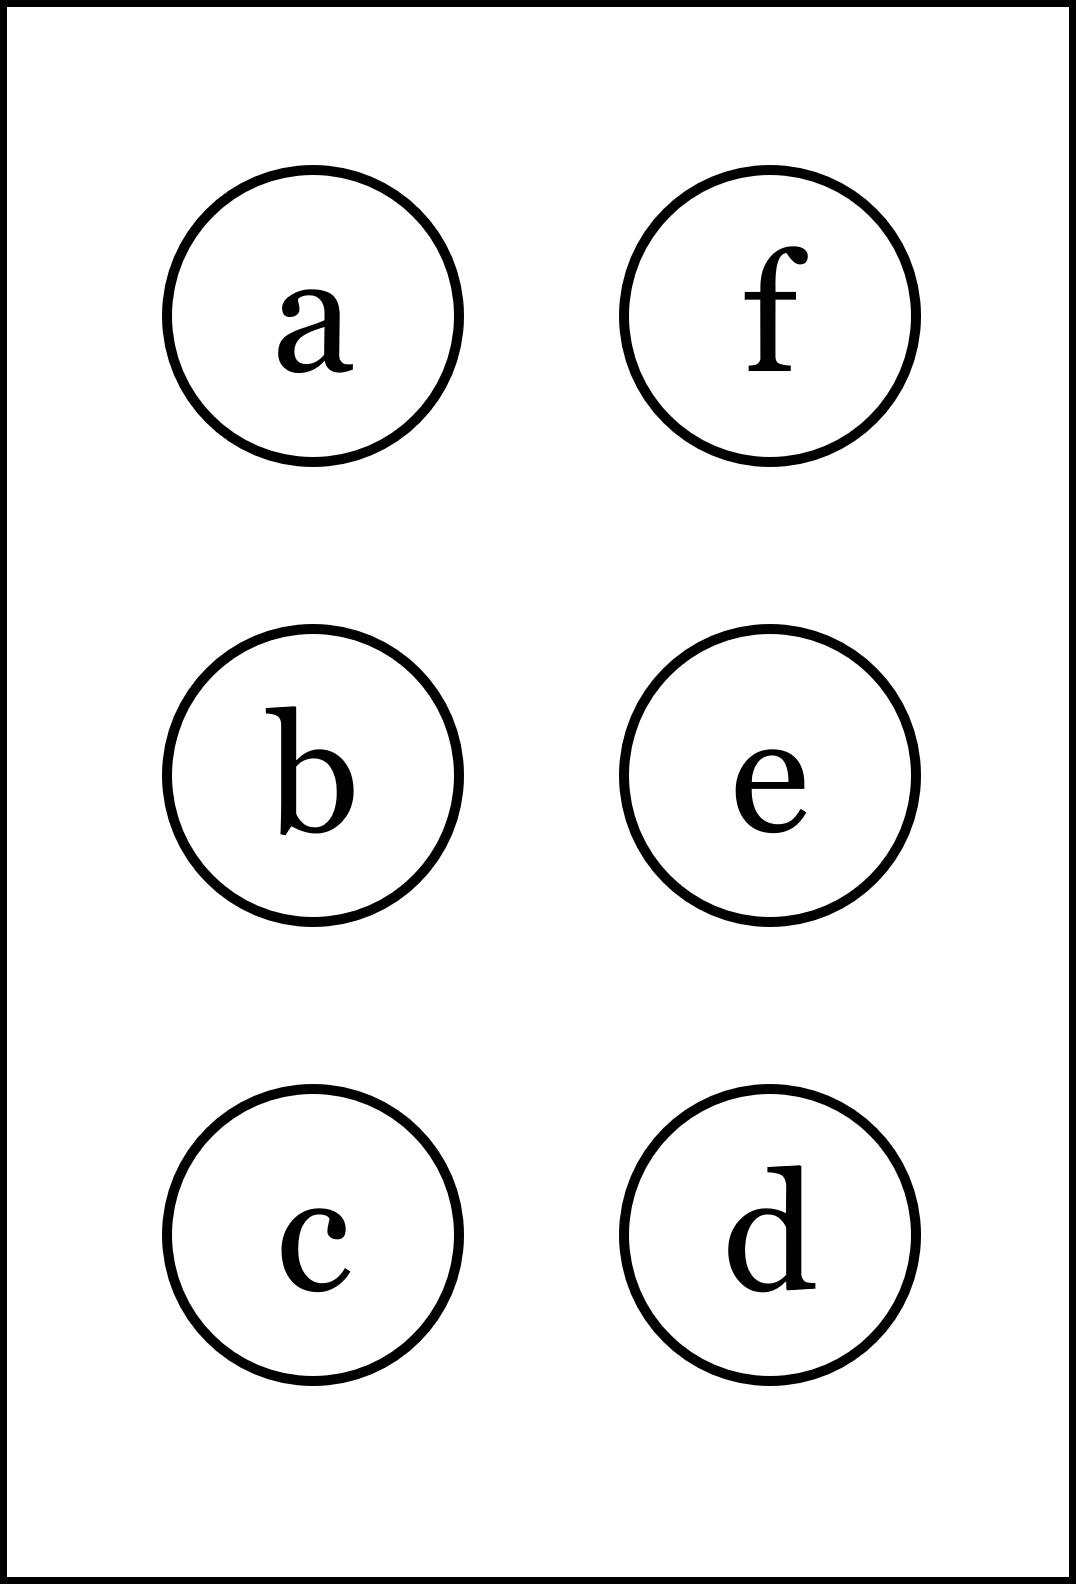
\includegraphics[height=40mm]{../images/braille.png}
{\small Písmeno Braillovej abecedy}
\end{center}
\end{minipage}
\end{center}
\end{minipage}
%
\end{tabular}
\newpage
\thispagestyle{empty}
\begin{tabular}{c:c}
\begin{minipage}[c][104.5mm][t]{0.5\linewidth}
\begin{center}
\vspace{7mm}
{\huge Kvadratická rovnice, skupina \textit{Theta $\theta$} -\romannumeral1}\\[5mm]
\textit{Jméno:}\phantom{xxxxxxxxxxxxxxxxxxxxxxxxxxxxxxxxxxxxxxxxxxxxxxxxxxxxxxxxxxxxxxxxx}\\[5mm]
\begin{minipage}{0.95\linewidth}
\begin{center}
V \textbf{(a)} a \textbf{(b)} zjisti počet řešení. V \textbf{(c)} x-ovú polohu vrcholu, a v \textbf{(d)} y-ovú polohu vrcholu.\\V \textbf{(e)} a \textbf{(f)} zjisti součet řešení. Pokud ti vyjde stejný výsledek jako je za otazníky, tak\\napravo obarvi příslušející kroužek načerno. \textbf{Spolu odevzdejte výsledné slovo}.
\end{center}
\end{minipage}
\\[1mm]
\begin{minipage}{0.79\linewidth}
\begin{center}
\begin{varwidth}{\linewidth}
\begin{enumerate}
\Large
\item $-2x^2-3x+4=0$\quad \dotfill\; ???\;\dotfill \quad 2
\item $-2x^2-2x+3=0$\quad \dotfill\; ???\;\dotfill \quad 0
\item $f(x)=x^2+6x-3$\quad \dotfill\; ???\;\dotfill \quad $-3$
\item $f(x)=5x^2-7x+1$\quad \dotfill\; ???\;\dotfill \quad $\nicefrac{-39}{20}$
\item $4x^2-20x+24=0$\quad \dotfill\; ???\;\dotfill \quad 7
\item $10x^2+11x+3=0$\quad \dotfill\; ???\;\dotfill \quad $\nicefrac{-11}{10}$
\end{enumerate}
\end{varwidth}
\end{center}
\end{minipage}
\begin{minipage}{0.20\linewidth}
\begin{center}
{\Huge\bfseries 1.} \\[2mm]
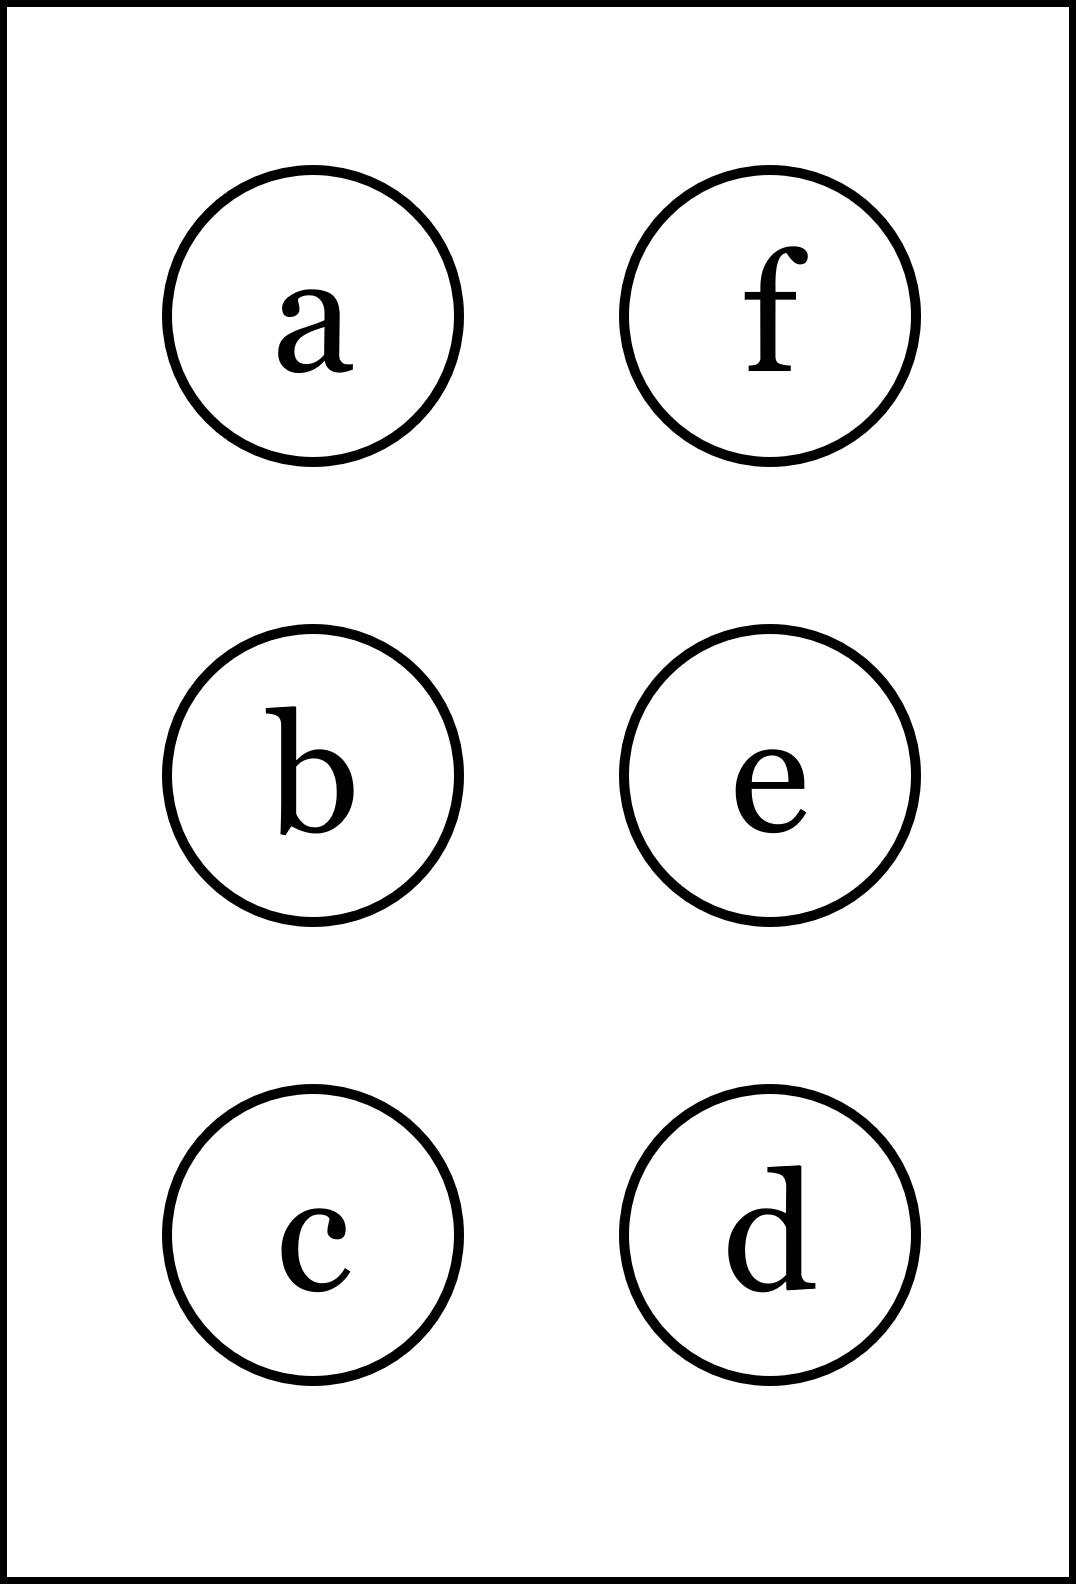
\includegraphics[height=40mm]{../images/braille.png}
{\small Písmeno Braillovej abecedy}
\end{center}
\end{minipage}
\end{center}
\end{minipage}
&
\begin{minipage}[c][104.5mm][t]{0.5\linewidth}
\begin{center}
\vspace{7mm}
{\huge Kvadratická rovnice, skupina \textit{Theta $\theta$} -\romannumeral2}\\[5mm]
\textit{Jméno:}\phantom{xxxxxxxxxxxxxxxxxxxxxxxxxxxxxxxxxxxxxxxxxxxxxxxxxxxxxxxxxxxxxxxxx}\\[5mm]
\begin{minipage}{0.95\linewidth}
\begin{center}
V \textbf{(a)} a \textbf{(b)} zjisti počet řešení. V \textbf{(c)} x-ovú polohu vrcholu, a v \textbf{(d)} y-ovú polohu vrcholu.\\V \textbf{(e)} a \textbf{(f)} zjisti součet řešení. Pokud ti vyjde stejný výsledek jako je za otazníky, tak\\napravo obarvi příslušející kroužek načerno. \textbf{Spolu odevzdejte výsledné slovo}.
\end{center}
\end{minipage}
\\[1mm]
\begin{minipage}{0.79\linewidth}
\begin{center}
\begin{varwidth}{\linewidth}
\begin{enumerate}
\Large
\item $2x^2-6x+4=0$\quad \dotfill\; ???\;\dotfill \quad 2
\item $x^2+x+1=0$\quad \dotfill\; ???\;\dotfill \quad 0
\item $f(x)=-5x^2-2x-3$\quad \dotfill\; ???\;\dotfill \quad $\nicefrac{-1}{5}$
\item $f(x)=2x^2+4x-5$\quad \dotfill\; ???\;\dotfill \quad $\nicefrac{-9}{2}$
\item $-6x^2-12x+18=0$\quad \dotfill\; ???\;\dotfill \quad -2
\item $-x^2-5x+24=0$\quad \dotfill\; ???\;\dotfill \quad $-11$
\end{enumerate}
\end{varwidth}
\end{center}
\end{minipage}
\begin{minipage}{0.20\linewidth}
\begin{center}
{\Huge\bfseries 2.} \\[2mm]
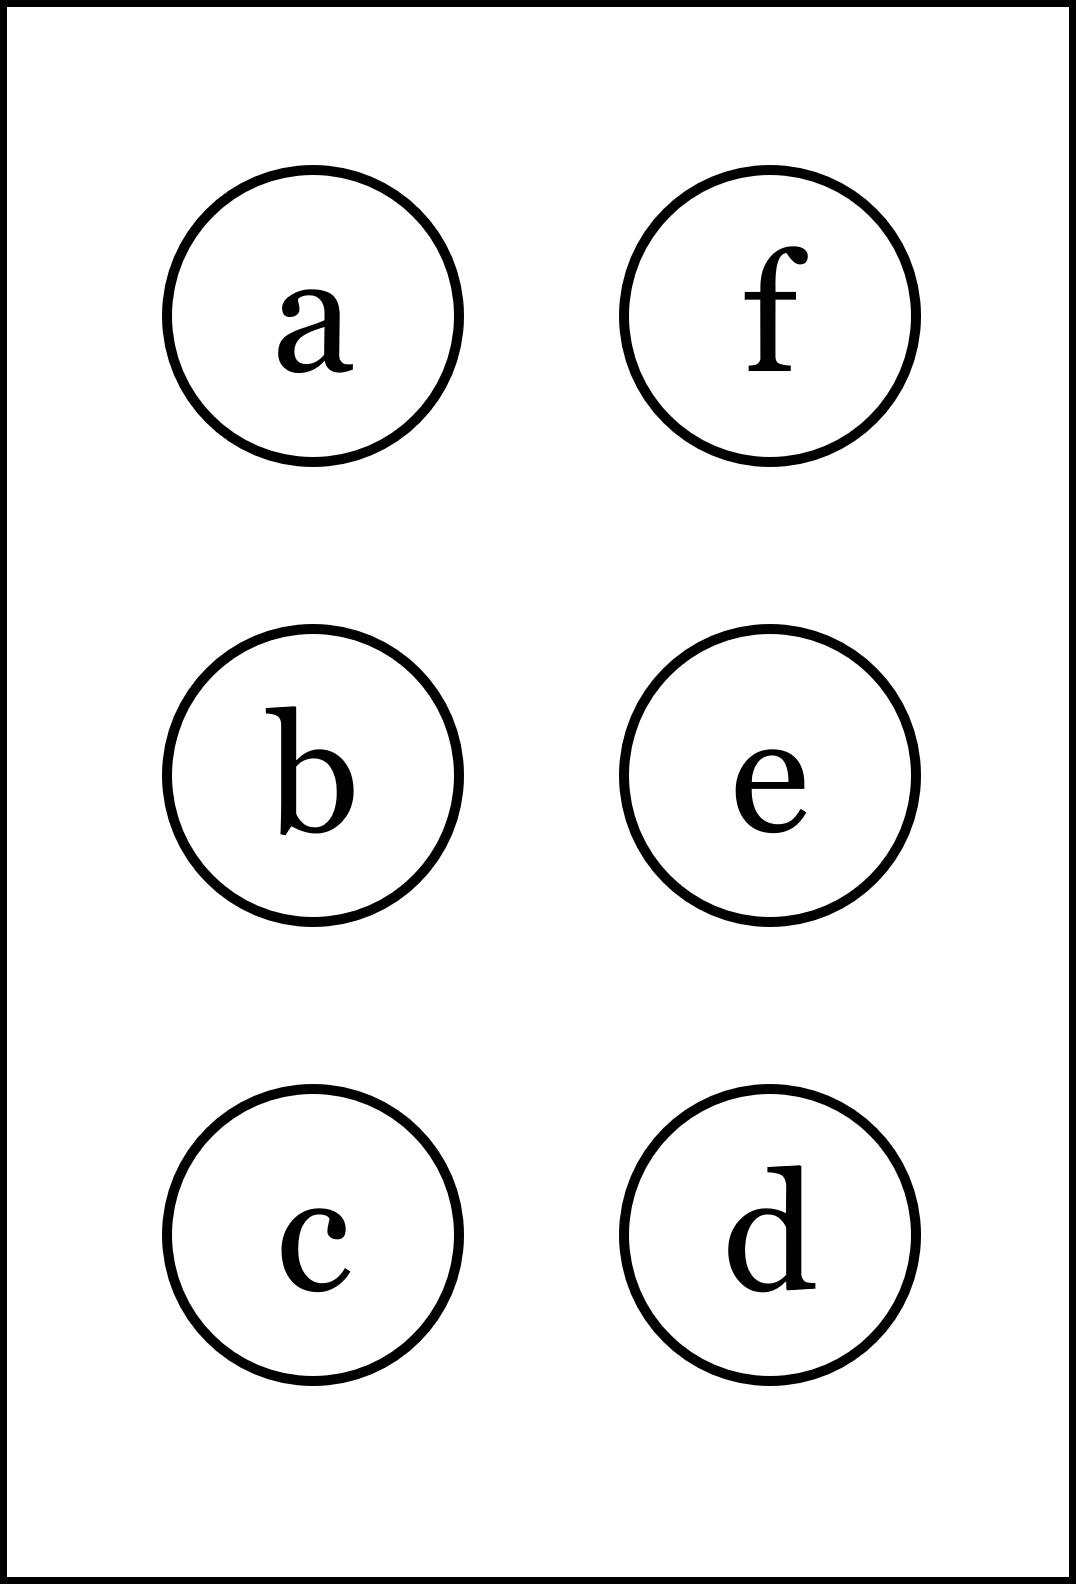
\includegraphics[height=40mm]{../images/braille.png}
{\small Písmeno Braillovej abecedy}
\end{center}
\end{minipage}
\end{center}
\end{minipage}
\\ \hdashline
\begin{minipage}[c][104.5mm][t]{0.5\linewidth}
\begin{center}
\vspace{7mm}
{\huge Kvadratická rovnice, skupina \textit{Theta $\theta$} -\romannumeral3}\\[5mm]
\textit{Jméno:}\phantom{xxxxxxxxxxxxxxxxxxxxxxxxxxxxxxxxxxxxxxxxxxxxxxxxxxxxxxxxxxxxxxxxx}\\[5mm]
\begin{minipage}{0.95\linewidth}
\begin{center}
V \textbf{(a)} a \textbf{(b)} zjisti počet řešení. V \textbf{(c)} x-ovú polohu vrcholu, a v \textbf{(d)} y-ovú polohu vrcholu.\\V \textbf{(e)} a \textbf{(f)} zjisti součet řešení. Pokud ti vyjde stejný výsledek jako je za otazníky, tak\\napravo obarvi příslušející kroužek načerno. \textbf{Spolu odevzdejte výsledné slovo}.
\end{center}
\end{minipage}
\\[1mm]
\begin{minipage}{0.79\linewidth}
\begin{center}
\begin{varwidth}{\linewidth}
\begin{enumerate}
\Large
\item $-7x^2-x-1=0$\quad \dotfill\; ???\;\dotfill \quad 0
\item $6x^2-2x-4=0$\quad \dotfill\; ???\;\dotfill \quad 0
\item $f(x)=-x^2+9x-1$\quad \dotfill\; ???\;\dotfill \quad $\nicefrac{-9}{2}$
\item $f(x)=-x^2+5x-6$\quad \dotfill\; ???\;\dotfill \quad $\nicefrac{13}{4}$
\item $-4x^2+20x-24=0$\quad \dotfill\; ???\;\dotfill \quad 4
\item $-2x^2-5x+12=0$\quad \dotfill\; ???\;\dotfill \quad $\nicefrac{11}{2}$
\end{enumerate}
\end{varwidth}
\end{center}
\end{minipage}
\begin{minipage}{0.20\linewidth}
\begin{center}
{\Huge\bfseries 3.} \\[2mm]
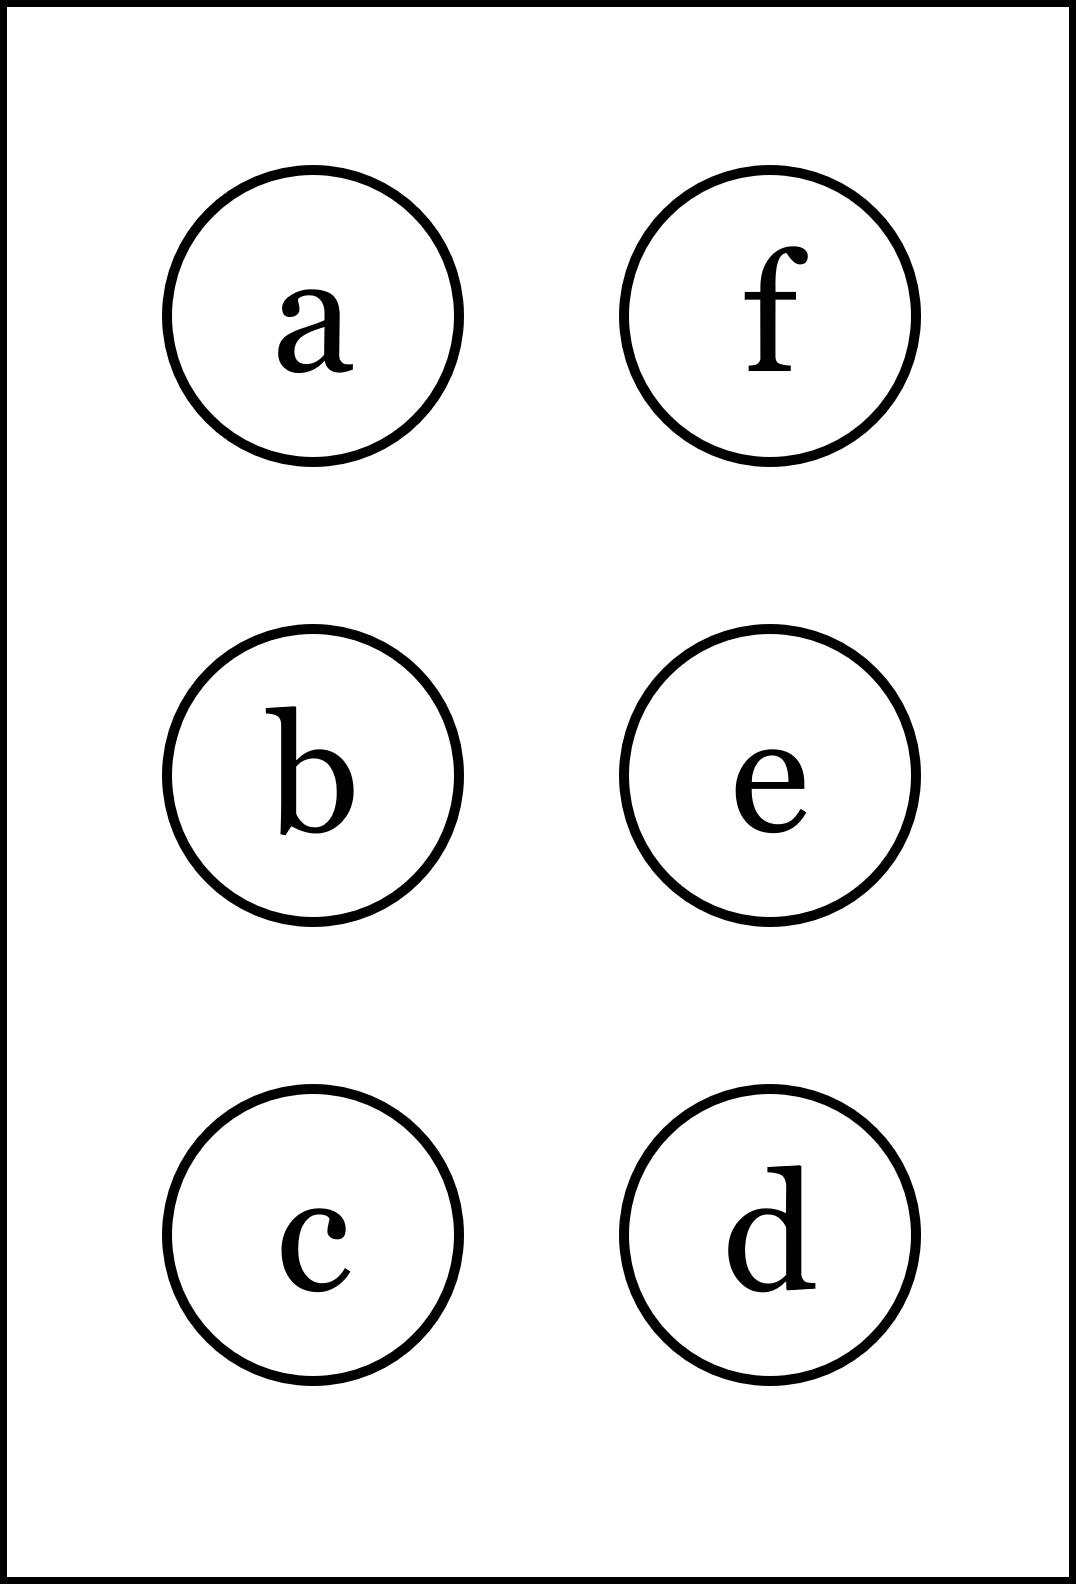
\includegraphics[height=40mm]{../images/braille.png}
{\small Písmeno Braillovej abecedy}
\end{center}
\end{minipage}
\end{center}
\end{minipage}
&
\begin{minipage}[c][104.5mm][t]{0.5\linewidth}
\begin{center}
\vspace{7mm}
{\huge Kvadratická rovnice, skupina \textit{Theta $\theta$} -\romannumeral4}\\[5mm]
\textit{Jméno:}\phantom{xxxxxxxxxxxxxxxxxxxxxxxxxxxxxxxxxxxxxxxxxxxxxxxxxxxxxxxxxxxxxxxxx}\\[5mm]
\begin{minipage}{0.95\linewidth}
\begin{center}
V \textbf{(a)} a \textbf{(b)} zjisti počet řešení. V \textbf{(c)} x-ovú polohu vrcholu, a v \textbf{(d)} y-ovú polohu vrcholu.\\V \textbf{(e)} a \textbf{(f)} zjisti součet řešení. Pokud ti vyjde stejný výsledek jako je za otazníky, tak\\napravo obarvi příslušející kroužek načerno. \textbf{Spolu odevzdejte výsledné slovo}.
\end{center}
\end{minipage}
\\[1mm]
\begin{minipage}{0.79\linewidth}
\begin{center}
\begin{varwidth}{\linewidth}
\begin{enumerate}
\Large
\item $5x^2-6x+1=0$\quad \dotfill\; ???\;\dotfill \quad 2
\item $5x^2+x+1=0$\quad \dotfill\; ???\;\dotfill \quad 1
\item $f(x)=-8x^2+x-5$\quad \dotfill\; ???\;\dotfill \quad $\nicefrac{1}{16}$
\item $f(x)=-7x^2+x+2$\quad \dotfill\; ???\;\dotfill \quad $\nicefrac{29}{28}$
\item $2x^2-6x+4=0$\quad \dotfill\; ???\;\dotfill \quad 5
\item $3x^2+7x-6=0$\quad \dotfill\; ???\;\dotfill \quad $\nicefrac{-11}{3}$
\end{enumerate}
\end{varwidth}
\end{center}
\end{minipage}
\begin{minipage}{0.20\linewidth}
\begin{center}
{\Huge\bfseries 4.} \\[2mm]
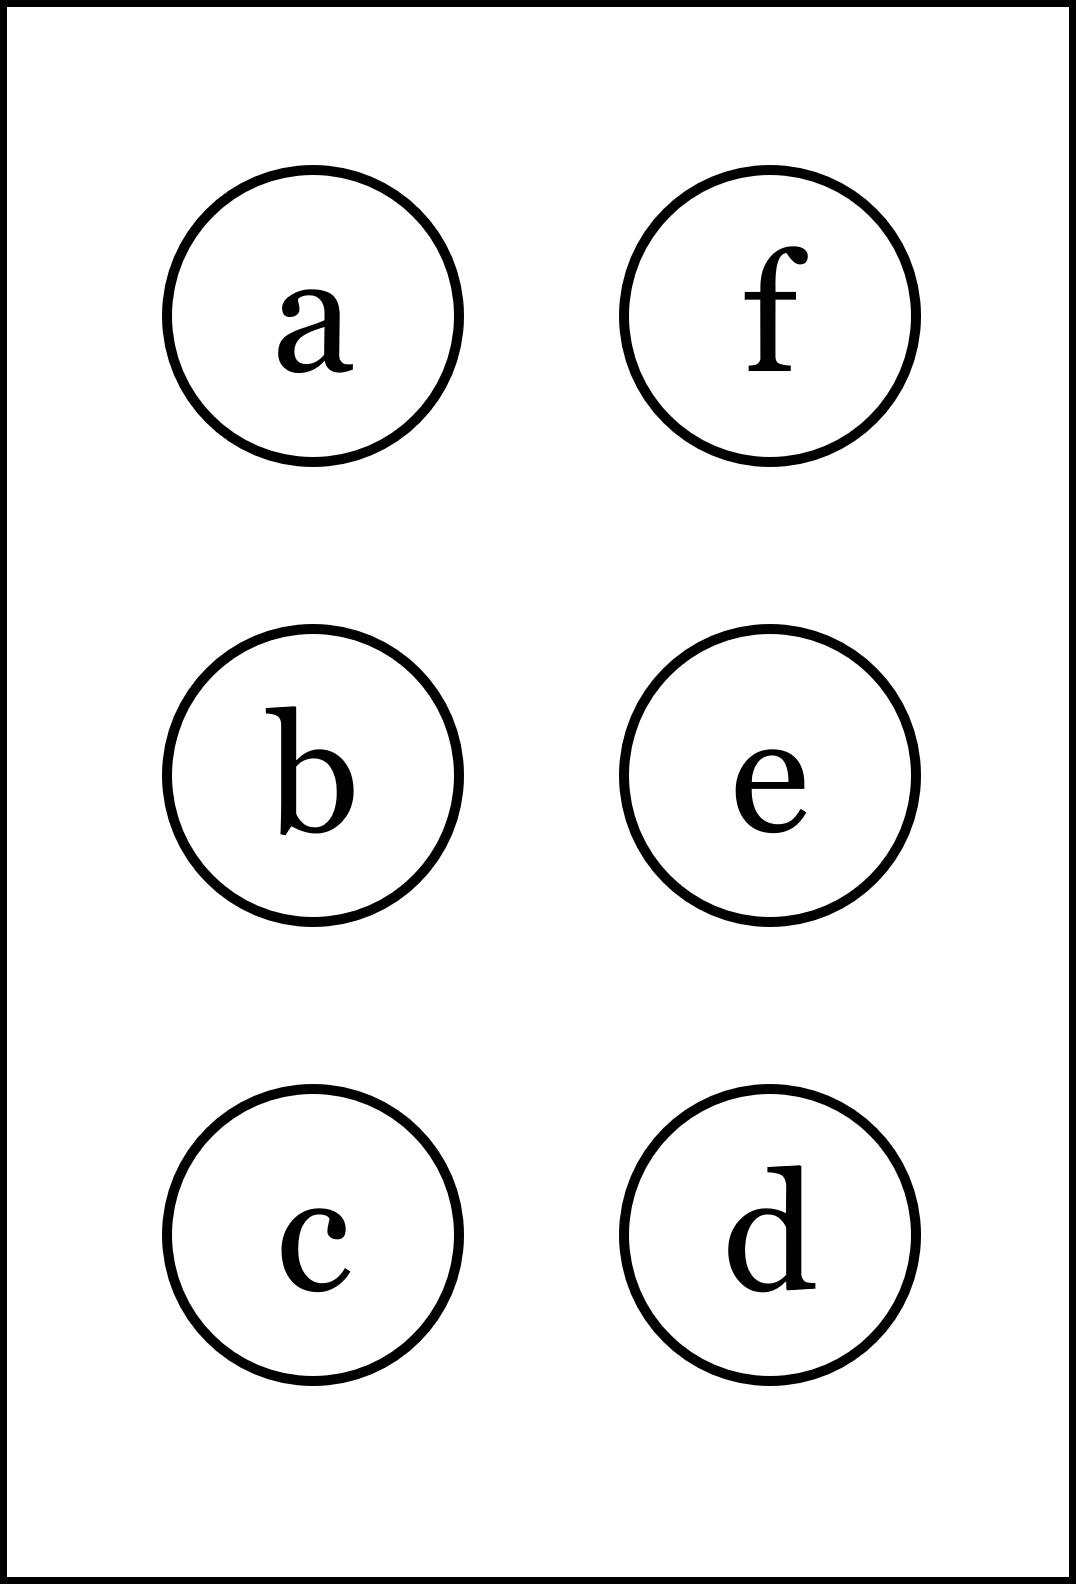
\includegraphics[height=40mm]{../images/braille.png}
{\small Písmeno Braillovej abecedy}
\end{center}
\end{minipage}
\end{center}
\end{minipage}
%
\end{tabular}
\newpage
\thispagestyle{empty}
\begin{tabular}{c:c}
\begin{minipage}[c][104.5mm][t]{0.5\linewidth}
\begin{center}
\vspace{7mm}
{\huge Kvadratická rovnice, skupina \textit{Iota $\iota$} -\romannumeral1}\\[5mm]
\textit{Jméno:}\phantom{xxxxxxxxxxxxxxxxxxxxxxxxxxxxxxxxxxxxxxxxxxxxxxxxxxxxxxxxxxxxxxxxx}\\[5mm]
\begin{minipage}{0.95\linewidth}
\begin{center}
V \textbf{(a)} a \textbf{(b)} zjisti počet řešení. V \textbf{(c)} x-ovú polohu vrcholu, a v \textbf{(d)} y-ovú polohu vrcholu.\\V \textbf{(e)} a \textbf{(f)} zjisti součet řešení. Pokud ti vyjde stejný výsledek jako je za otazníky, tak\\napravo obarvi příslušející kroužek načerno. \textbf{Spolu odevzdejte výsledné slovo}.
\end{center}
\end{minipage}
\\[1mm]
\begin{minipage}{0.79\linewidth}
\begin{center}
\begin{varwidth}{\linewidth}
\begin{enumerate}
\Large
\item $x^2-2x+7=0$\quad \dotfill\; ???\;\dotfill \quad 1
\item $-2x^2+2x+2=0$\quad \dotfill\; ???\;\dotfill \quad 2
\item $f(x)=-4x^2-x+1$\quad \dotfill\; ???\;\dotfill \quad $\nicefrac{-1}{8}$
\item $f(x)=-4x^2+7x+3$\quad \dotfill\; ???\;\dotfill \quad $\nicefrac{73}{16}$
\item $-x^2-6x-8=0$\quad \dotfill\; ???\;\dotfill \quad -9
\item $-6x^2+16x-10=0$\quad \dotfill\; ???\;\dotfill \quad $\nicefrac{8}{3}$
\end{enumerate}
\end{varwidth}
\end{center}
\end{minipage}
\begin{minipage}{0.20\linewidth}
\begin{center}
{\Huge\bfseries 1.} \\[2mm]
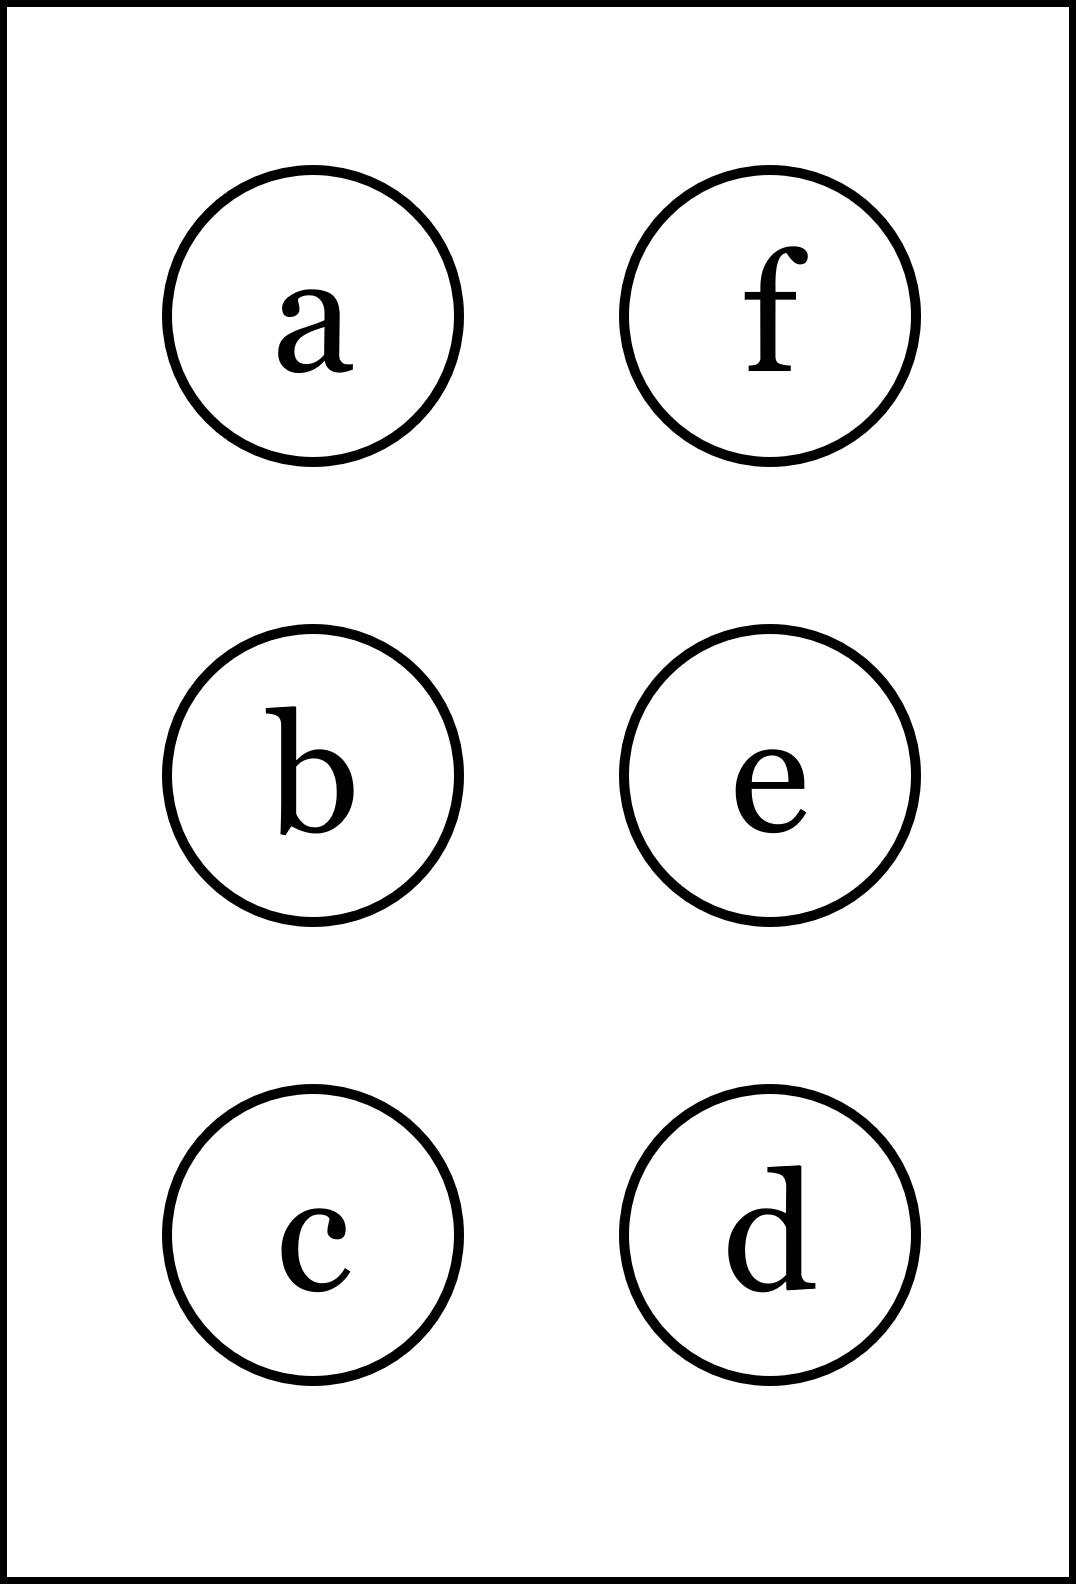
\includegraphics[height=40mm]{../images/braille.png}
{\small Písmeno Braillovej abecedy}
\end{center}
\end{minipage}
\end{center}
\end{minipage}
&
\begin{minipage}[c][104.5mm][t]{0.5\linewidth}
\begin{center}
\vspace{7mm}
{\huge Kvadratická rovnice, skupina \textit{Iota $\iota$} -\romannumeral2}\\[5mm]
\textit{Jméno:}\phantom{xxxxxxxxxxxxxxxxxxxxxxxxxxxxxxxxxxxxxxxxxxxxxxxxxxxxxxxxxxxxxxxxx}\\[5mm]
\begin{minipage}{0.95\linewidth}
\begin{center}
V \textbf{(a)} a \textbf{(b)} zjisti počet řešení. V \textbf{(c)} x-ovú polohu vrcholu, a v \textbf{(d)} y-ovú polohu vrcholu.\\V \textbf{(e)} a \textbf{(f)} zjisti součet řešení. Pokud ti vyjde stejný výsledek jako je za otazníky, tak\\napravo obarvi příslušející kroužek načerno. \textbf{Spolu odevzdejte výsledné slovo}.
\end{center}
\end{minipage}
\\[1mm]
\begin{minipage}{0.79\linewidth}
\begin{center}
\begin{varwidth}{\linewidth}
\begin{enumerate}
\Large
\item $-6x^2-x-4=0$\quad \dotfill\; ???\;\dotfill \quad 0
\item $-x^2+5x-5=0$\quad \dotfill\; ???\;\dotfill \quad 0
\item $f(x)=5x^2+3x+8$\quad \dotfill\; ???\;\dotfill \quad $\nicefrac{3}{10}$
\item $f(x)=2x^2-2x+1$\quad \dotfill\; ???\;\dotfill \quad $0$
\item $-2x^2+18x-36=0$\quad \dotfill\; ???\;\dotfill \quad 9
\item $-24x^2+5x+1=0$\quad \dotfill\; ???\;\dotfill \quad $\nicefrac{11}{24}$
\end{enumerate}
\end{varwidth}
\end{center}
\end{minipage}
\begin{minipage}{0.20\linewidth}
\begin{center}
{\Huge\bfseries 2.} \\[2mm]
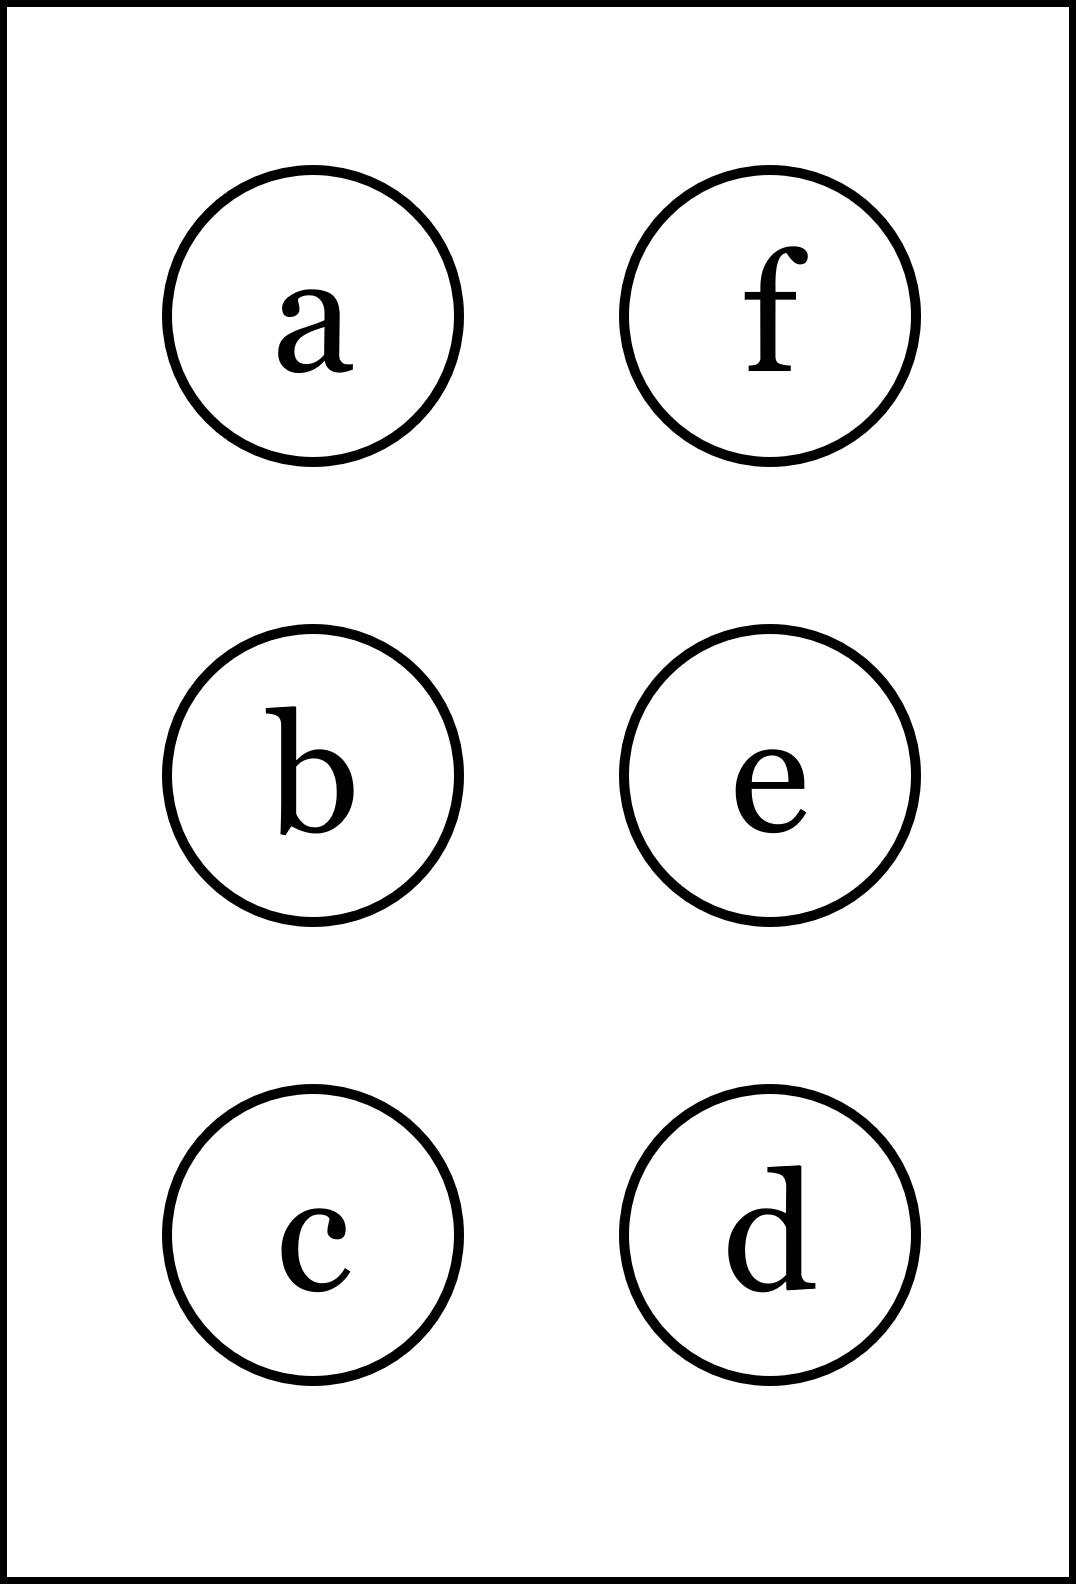
\includegraphics[height=40mm]{../images/braille.png}
{\small Písmeno Braillovej abecedy}
\end{center}
\end{minipage}
\end{center}
\end{minipage}
\\ \hdashline
\begin{minipage}[c][104.5mm][t]{0.5\linewidth}
\begin{center}
\vspace{7mm}
{\huge Kvadratická rovnice, skupina \textit{Iota $\iota$} -\romannumeral3}\\[5mm]
\textit{Jméno:}\phantom{xxxxxxxxxxxxxxxxxxxxxxxxxxxxxxxxxxxxxxxxxxxxxxxxxxxxxxxxxxxxxxxxx}\\[5mm]
\begin{minipage}{0.95\linewidth}
\begin{center}
V \textbf{(a)} a \textbf{(b)} zjisti počet řešení. V \textbf{(c)} x-ovú polohu vrcholu, a v \textbf{(d)} y-ovú polohu vrcholu.\\V \textbf{(e)} a \textbf{(f)} zjisti součet řešení. Pokud ti vyjde stejný výsledek jako je za otazníky, tak\\napravo obarvi příslušející kroužek načerno. \textbf{Spolu odevzdejte výsledné slovo}.
\end{center}
\end{minipage}
\\[1mm]
\begin{minipage}{0.79\linewidth}
\begin{center}
\begin{varwidth}{\linewidth}
\begin{enumerate}
\Large
\item $3x^2+3x-2=0$\quad \dotfill\; ???\;\dotfill \quad 2
\item $4x^2+2x+3=0$\quad \dotfill\; ???\;\dotfill \quad 1
\item $f(x)=4x^2+3x+9$\quad \dotfill\; ???\;\dotfill \quad $\nicefrac{-3}{8}$
\item $f(x)=-5x^2+6x-5$\quad \dotfill\; ???\;\dotfill \quad $\nicefrac{-7}{10}$
\item $4x^2-12x+8=0$\quad \dotfill\; ???\;\dotfill \quad 3
\item $x^2+x-2=0$\quad \dotfill\; ???\;\dotfill \quad $-1$
\end{enumerate}
\end{varwidth}
\end{center}
\end{minipage}
\begin{minipage}{0.20\linewidth}
\begin{center}
{\Huge\bfseries 3.} \\[2mm]
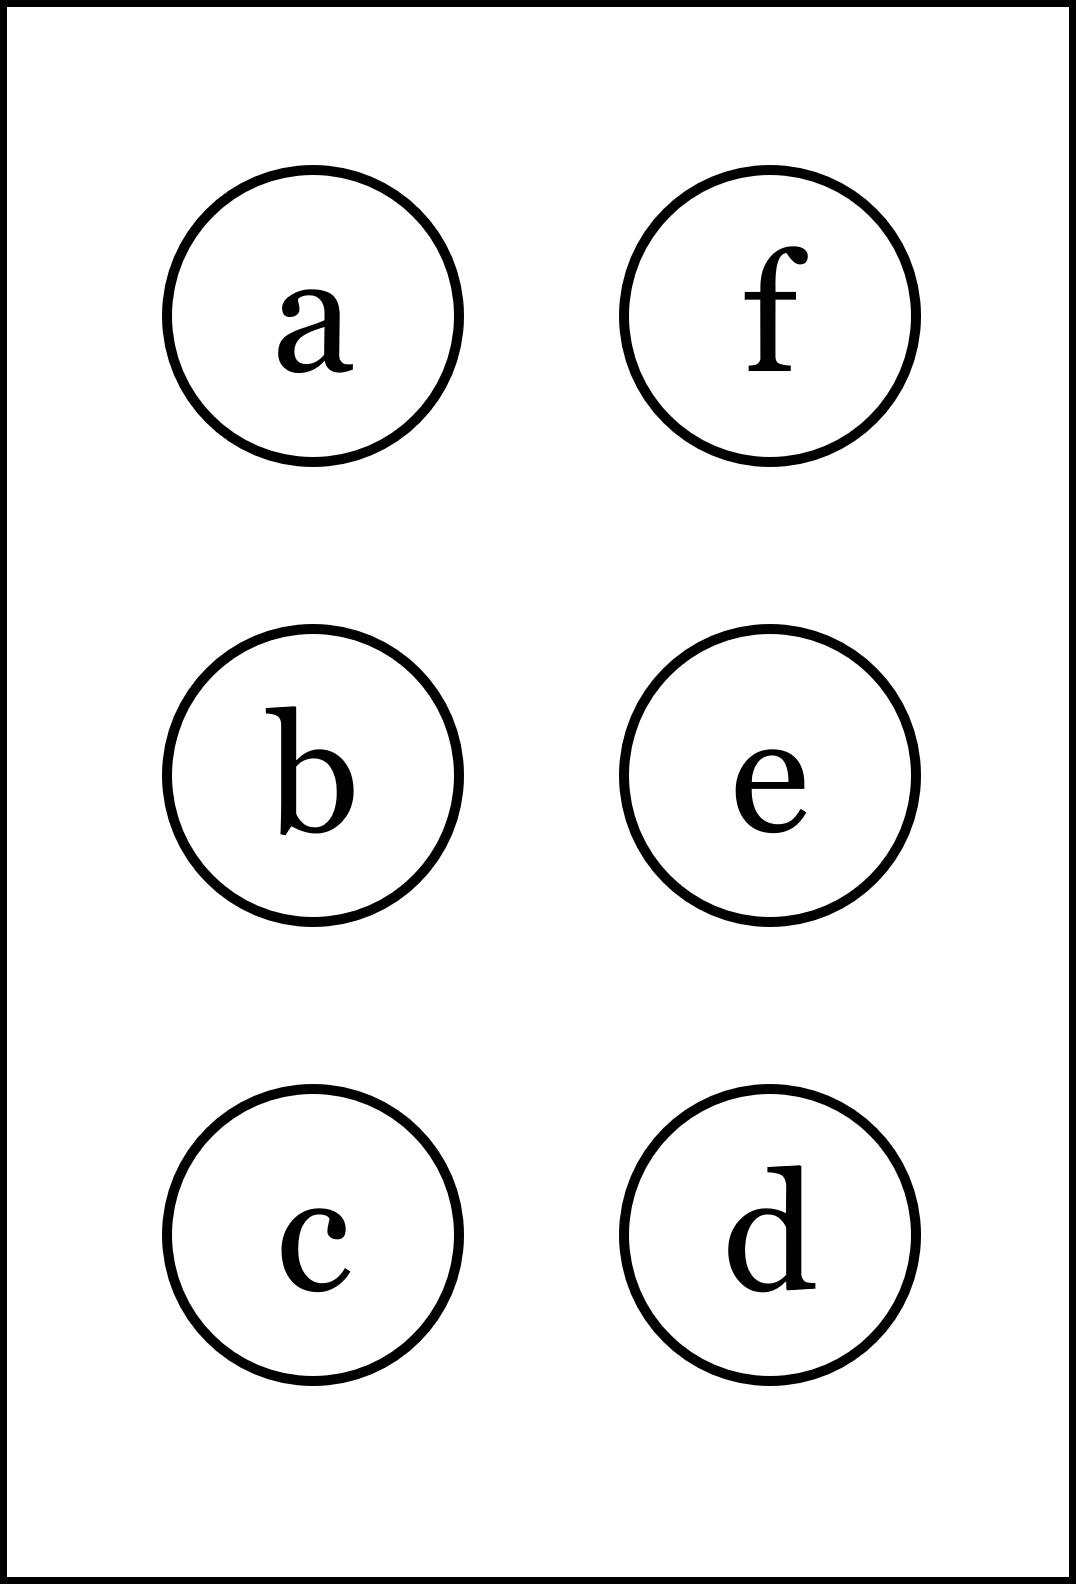
\includegraphics[height=40mm]{../images/braille.png}
{\small Písmeno Braillovej abecedy}
\end{center}
\end{minipage}
\end{center}
\end{minipage}
&
\begin{minipage}[c][104.5mm][t]{0.5\linewidth}
\begin{center}
\vspace{7mm}
{\huge Kvadratická rovnice, skupina \textit{Iota $\iota$} -\romannumeral4}\\[5mm]
\textit{Jméno:}\phantom{xxxxxxxxxxxxxxxxxxxxxxxxxxxxxxxxxxxxxxxxxxxxxxxxxxxxxxxxxxxxxxxxx}\\[5mm]
\begin{minipage}{0.95\linewidth}
\begin{center}
V \textbf{(a)} a \textbf{(b)} zjisti počet řešení. V \textbf{(c)} x-ovú polohu vrcholu, a v \textbf{(d)} y-ovú polohu vrcholu.\\V \textbf{(e)} a \textbf{(f)} zjisti součet řešení. Pokud ti vyjde stejný výsledek jako je za otazníky, tak\\napravo obarvi příslušející kroužek načerno. \textbf{Spolu odevzdejte výsledné slovo}.
\end{center}
\end{minipage}
\\[1mm]
\begin{minipage}{0.79\linewidth}
\begin{center}
\begin{varwidth}{\linewidth}
\begin{enumerate}
\Large
\item $7x^2+6x-1=0$\quad \dotfill\; ???\;\dotfill \quad 2
\item $3x^2+5x-8=0$\quad \dotfill\; ???\;\dotfill \quad 1
\item $f(x)=-9x^2+7x-2$\quad \dotfill\; ???\;\dotfill \quad $\nicefrac{7}{18}$
\item $f(x)=-2x^2+3x-2$\quad \dotfill\; ???\;\dotfill \quad $\nicefrac{1}{8}$
\item $-4x^2+16x-12=0$\quad \dotfill\; ???\;\dotfill \quad 4
\item $2x^2+7x+6=0$\quad \dotfill\; ???\;\dotfill \quad $\nicefrac{-1}{2}$
\end{enumerate}
\end{varwidth}
\end{center}
\end{minipage}
\begin{minipage}{0.20\linewidth}
\begin{center}
{\Huge\bfseries 4.} \\[2mm]
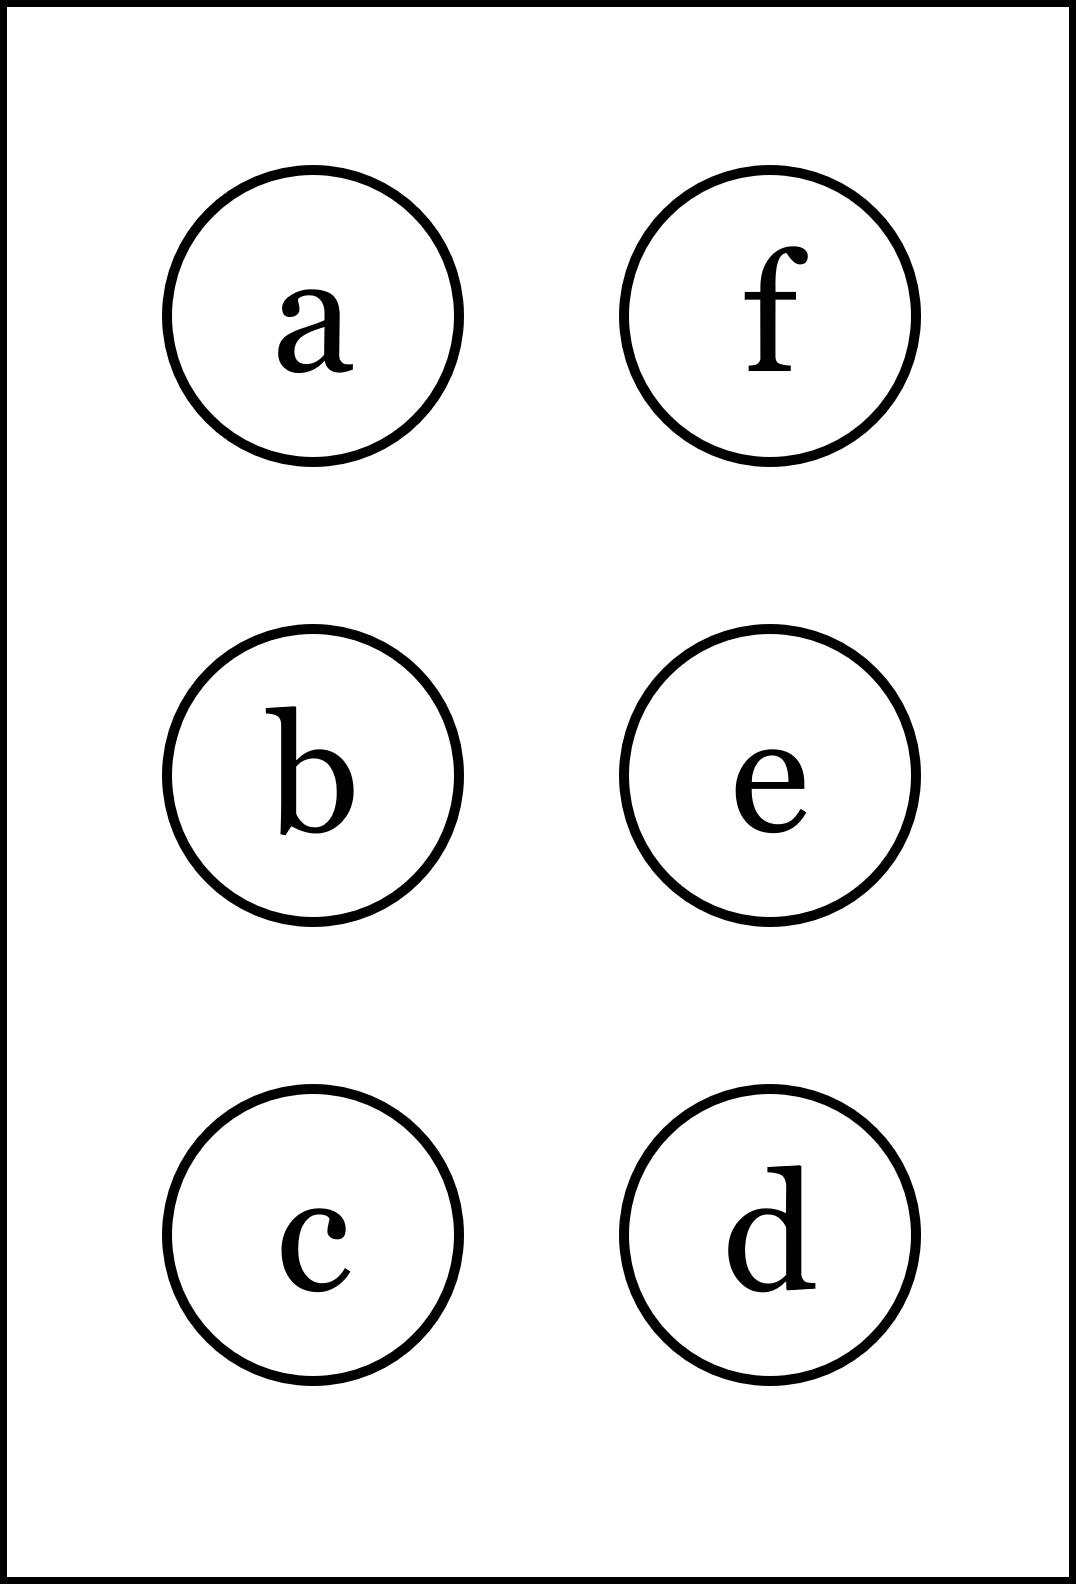
\includegraphics[height=40mm]{../images/braille.png}
{\small Písmeno Braillovej abecedy}
\end{center}
\end{minipage}
\end{center}
\end{minipage}
%
\end{tabular}
\newpage
\thispagestyle{empty}
\begin{tabular}{c:c}
\begin{minipage}[c][104.5mm][t]{0.5\linewidth}
\begin{center}
\vspace{7mm}
{\huge Kvadratická rovnice, skupina \textit{Kappa $\kappa$} -\romannumeral1}\\[5mm]
\textit{Jméno:}\phantom{xxxxxxxxxxxxxxxxxxxxxxxxxxxxxxxxxxxxxxxxxxxxxxxxxxxxxxxxxxxxxxxxx}\\[5mm]
\begin{minipage}{0.95\linewidth}
\begin{center}
V \textbf{(a)} a \textbf{(b)} zjisti počet řešení. V \textbf{(c)} x-ovú polohu vrcholu, a v \textbf{(d)} y-ovú polohu vrcholu.\\V \textbf{(e)} a \textbf{(f)} zjisti součet řešení. Pokud ti vyjde stejný výsledek jako je za otazníky, tak\\napravo obarvi příslušející kroužek načerno. \textbf{Spolu odevzdejte výsledné slovo}.
\end{center}
\end{minipage}
\\[1mm]
\begin{minipage}{0.79\linewidth}
\begin{center}
\begin{varwidth}{\linewidth}
\begin{enumerate}
\Large
\item $2x^2-6x+3=0$\quad \dotfill\; ???\;\dotfill \quad 1
\item $2x^2-x-4=0$\quad \dotfill\; ???\;\dotfill \quad 2
\item $f(x)=-7x^2+4x-2$\quad \dotfill\; ???\;\dotfill \quad $\nicefrac{2}{7}$
\item $f(x)=-2x^2-2x-1$\quad \dotfill\; ???\;\dotfill \quad $\nicefrac{-1}{2}$
\item $8x^2-32x+24=0$\quad \dotfill\; ???\;\dotfill \quad 5
\item $x^2-4x-5=0$\quad \dotfill\; ???\;\dotfill \quad $4$
\end{enumerate}
\end{varwidth}
\end{center}
\end{minipage}
\begin{minipage}{0.20\linewidth}
\begin{center}
{\Huge\bfseries 1.} \\[2mm]
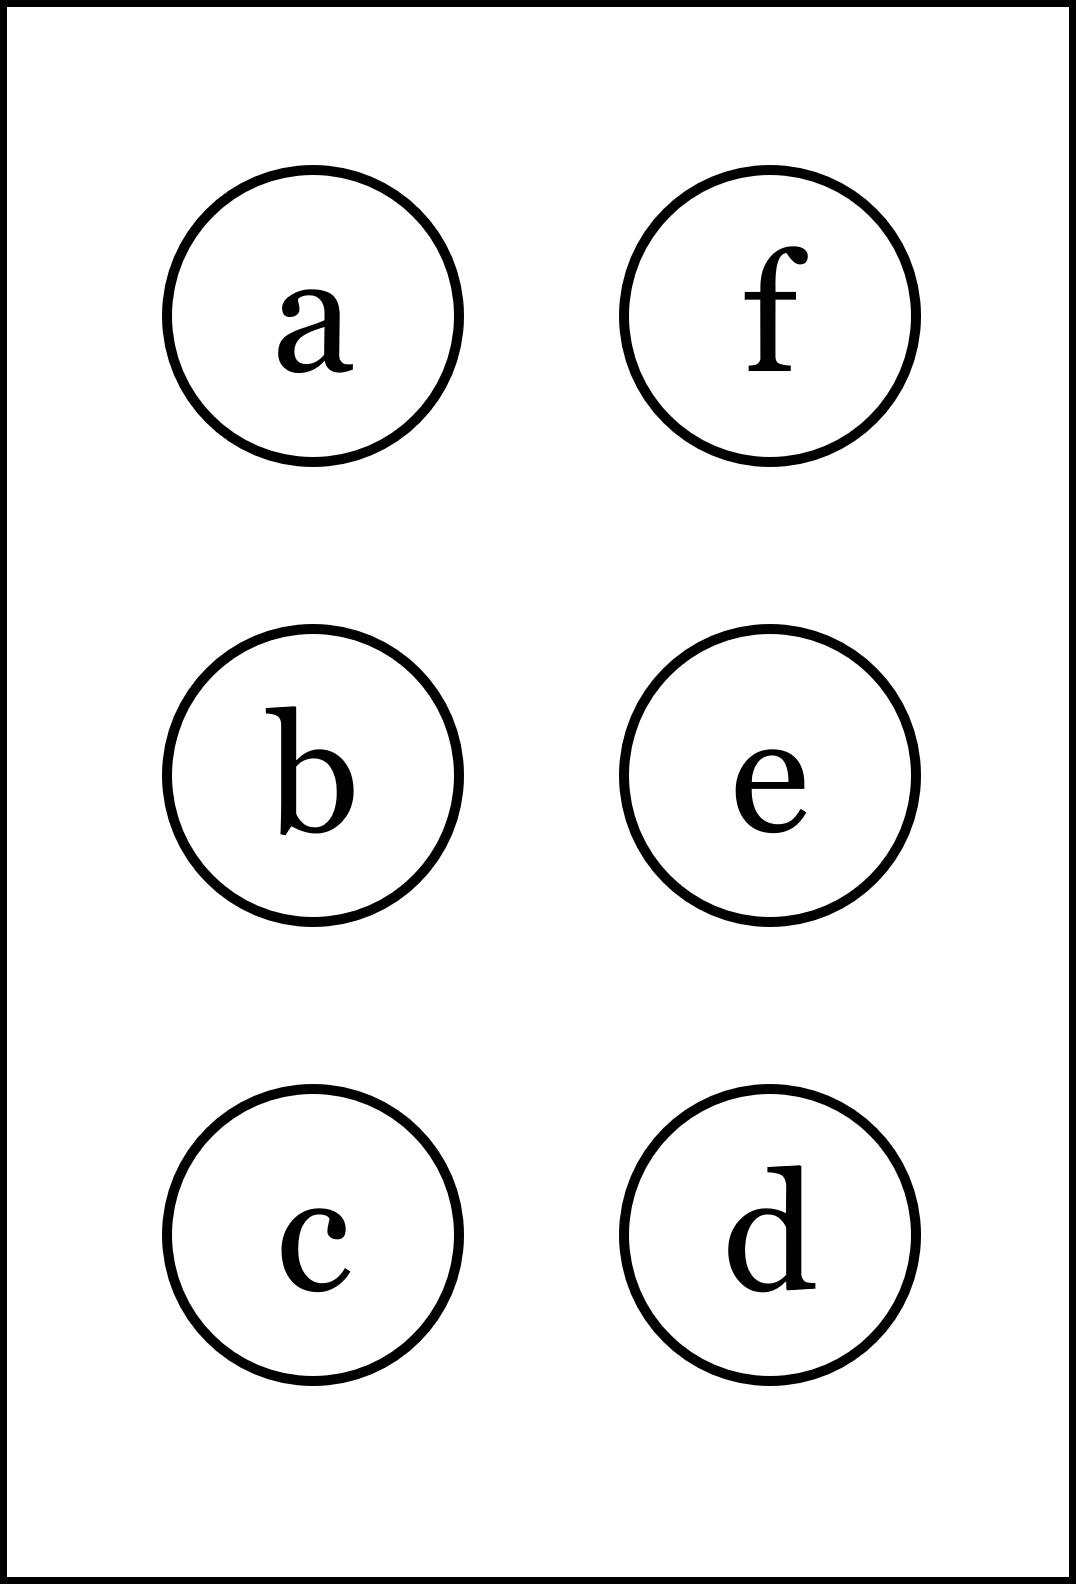
\includegraphics[height=40mm]{../images/braille.png}
{\small Písmeno Braillovej abecedy}
\end{center}
\end{minipage}
\end{center}
\end{minipage}
&
\begin{minipage}[c][104.5mm][t]{0.5\linewidth}
\begin{center}
\vspace{7mm}
{\huge Kvadratická rovnice, skupina \textit{Kappa $\kappa$} -\romannumeral2}\\[5mm]
\textit{Jméno:}\phantom{xxxxxxxxxxxxxxxxxxxxxxxxxxxxxxxxxxxxxxxxxxxxxxxxxxxxxxxxxxxxxxxxx}\\[5mm]
\begin{minipage}{0.95\linewidth}
\begin{center}
V \textbf{(a)} a \textbf{(b)} zjisti počet řešení. V \textbf{(c)} x-ovú polohu vrcholu, a v \textbf{(d)} y-ovú polohu vrcholu.\\V \textbf{(e)} a \textbf{(f)} zjisti součet řešení. Pokud ti vyjde stejný výsledek jako je za otazníky, tak\\napravo obarvi příslušející kroužek načerno. \textbf{Spolu odevzdejte výsledné slovo}.
\end{center}
\end{minipage}
\\[1mm]
\begin{minipage}{0.79\linewidth}
\begin{center}
\begin{varwidth}{\linewidth}
\begin{enumerate}
\Large
\item $2x^2-x-5=0$\quad \dotfill\; ???\;\dotfill \quad 2
\item $7x^2-7x+4=0$\quad \dotfill\; ???\;\dotfill \quad 1
\item $f(x)=-7x^2-x-8$\quad \dotfill\; ???\;\dotfill \quad $\nicefrac{1}{14}$
\item $f(x)=2x^2-8x+1$\quad \dotfill\; ???\;\dotfill \quad $-7$
\item $2x^2+8x-10=0$\quad \dotfill\; ???\;\dotfill \quad -5
\item $-2x^2+13x-15=0$\quad \dotfill\; ???\;\dotfill \quad $\nicefrac{-7}{2}$
\end{enumerate}
\end{varwidth}
\end{center}
\end{minipage}
\begin{minipage}{0.20\linewidth}
\begin{center}
{\Huge\bfseries 2.} \\[2mm]
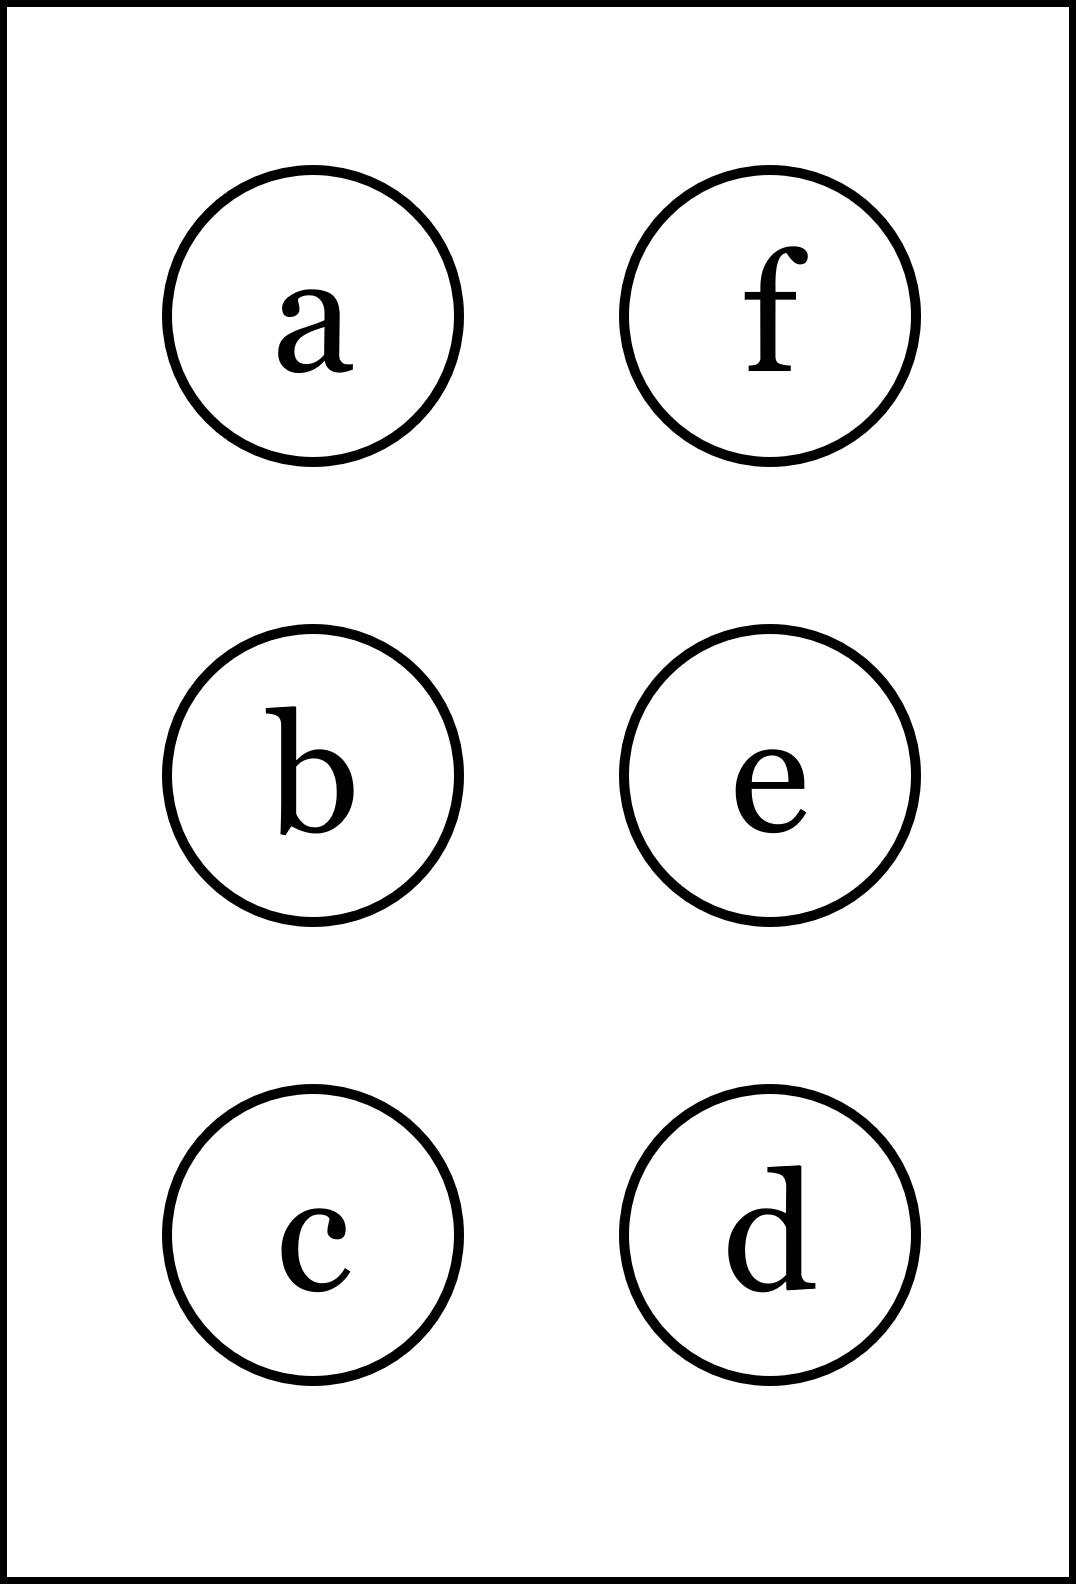
\includegraphics[height=40mm]{../images/braille.png}
{\small Písmeno Braillovej abecedy}
\end{center}
\end{minipage}
\end{center}
\end{minipage}
\\ \hdashline
\begin{minipage}[c][104.5mm][t]{0.5\linewidth}
\begin{center}
\vspace{7mm}
{\huge Kvadratická rovnice, skupina \textit{Kappa $\kappa$} -\romannumeral3}\\[5mm]
\textit{Jméno:}\phantom{xxxxxxxxxxxxxxxxxxxxxxxxxxxxxxxxxxxxxxxxxxxxxxxxxxxxxxxxxxxxxxxxx}\\[5mm]
\begin{minipage}{0.95\linewidth}
\begin{center}
V \textbf{(a)} a \textbf{(b)} zjisti počet řešení. V \textbf{(c)} x-ovú polohu vrcholu, a v \textbf{(d)} y-ovú polohu vrcholu.\\V \textbf{(e)} a \textbf{(f)} zjisti součet řešení. Pokud ti vyjde stejný výsledek jako je za otazníky, tak\\napravo obarvi příslušející kroužek načerno. \textbf{Spolu odevzdejte výsledné slovo}.
\end{center}
\end{minipage}
\\[1mm]
\begin{minipage}{0.79\linewidth}
\begin{center}
\begin{varwidth}{\linewidth}
\begin{enumerate}
\Large
\item $3x^2+2x+1=0$\quad \dotfill\; ???\;\dotfill \quad 0
\item $-5x^2+3x+8=0$\quad \dotfill\; ???\;\dotfill \quad 2
\item $f(x)=5x^2-3x+1$\quad \dotfill\; ???\;\dotfill \quad $\nicefrac{-3}{10}$
\item $f(x)=-2x^2+8x-8$\quad \dotfill\; ???\;\dotfill \quad $4$
\item $x^2-7x+10=0$\quad \dotfill\; ???\;\dotfill \quad 6
\item $-4x^2+11x-6=0$\quad \dotfill\; ???\;\dotfill \quad $\nicefrac{-5}{4}$
\end{enumerate}
\end{varwidth}
\end{center}
\end{minipage}
\begin{minipage}{0.20\linewidth}
\begin{center}
{\Huge\bfseries 3.} \\[2mm]
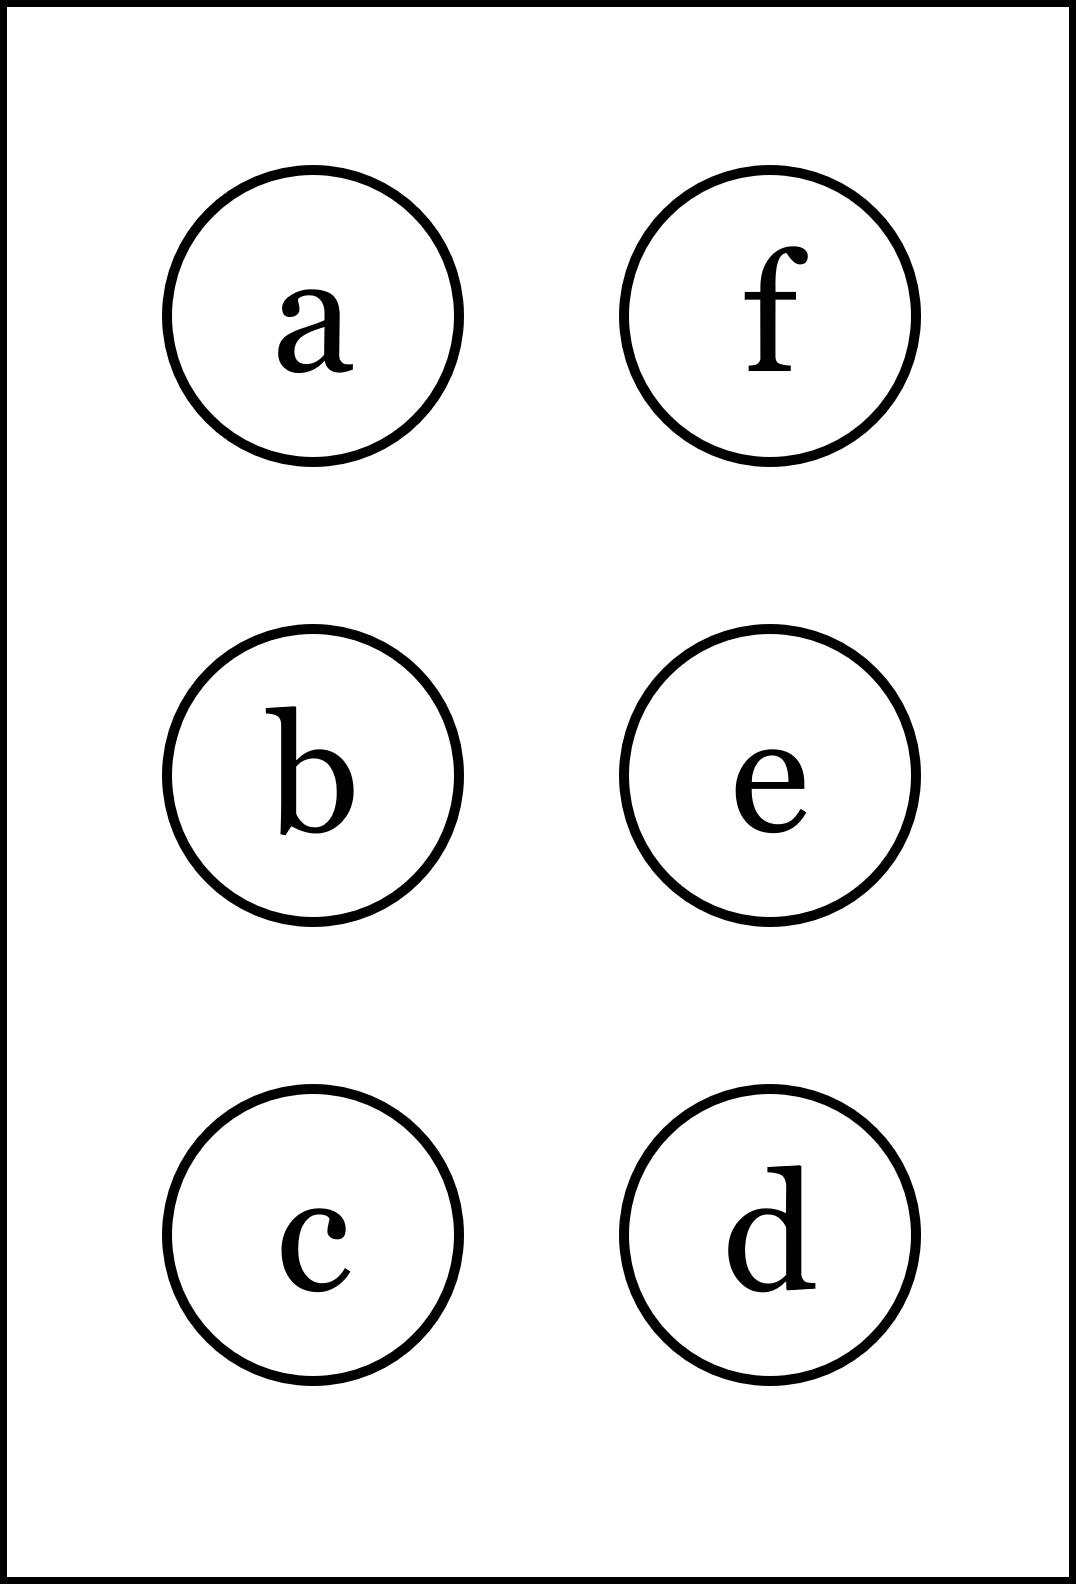
\includegraphics[height=40mm]{../images/braille.png}
{\small Písmeno Braillovej abecedy}
\end{center}
\end{minipage}
\end{center}
\end{minipage}
&
\begin{minipage}[c][104.5mm][t]{0.5\linewidth}
\begin{center}
\vspace{7mm}
{\huge Kvadratická rovnice, skupina \textit{Kappa $\kappa$} -\romannumeral4}\\[5mm]
\textit{Jméno:}\phantom{xxxxxxxxxxxxxxxxxxxxxxxxxxxxxxxxxxxxxxxxxxxxxxxxxxxxxxxxxxxxxxxxx}\\[5mm]
\begin{minipage}{0.95\linewidth}
\begin{center}
V \textbf{(a)} a \textbf{(b)} zjisti počet řešení. V \textbf{(c)} x-ovú polohu vrcholu, a v \textbf{(d)} y-ovú polohu vrcholu.\\V \textbf{(e)} a \textbf{(f)} zjisti součet řešení. Pokud ti vyjde stejný výsledek jako je za otazníky, tak\\napravo obarvi příslušející kroužek načerno. \textbf{Spolu odevzdejte výsledné slovo}.
\end{center}
\end{minipage}
\\[1mm]
\begin{minipage}{0.79\linewidth}
\begin{center}
\begin{varwidth}{\linewidth}
\begin{enumerate}
\Large
\item $-4x^2+2x-5=0$\quad \dotfill\; ???\;\dotfill \quad 0
\item $-x^2-4x+1=0$\quad \dotfill\; ???\;\dotfill \quad 1
\item $f(x)=5x^2-9x+1$\quad \dotfill\; ???\;\dotfill \quad $\nicefrac{-9}{10}$
\item $f(x)=3x^2+2x+7$\quad \dotfill\; ???\;\dotfill \quad $\nicefrac{19}{6}$
\item $-4x^2+12x-8=0$\quad \dotfill\; ???\;\dotfill \quad 6
\item $2x^2-9x+9=0$\quad \dotfill\; ???\;\dotfill \quad $\nicefrac{3}{2}$
\end{enumerate}
\end{varwidth}
\end{center}
\end{minipage}
\begin{minipage}{0.20\linewidth}
\begin{center}
{\Huge\bfseries 4.} \\[2mm]
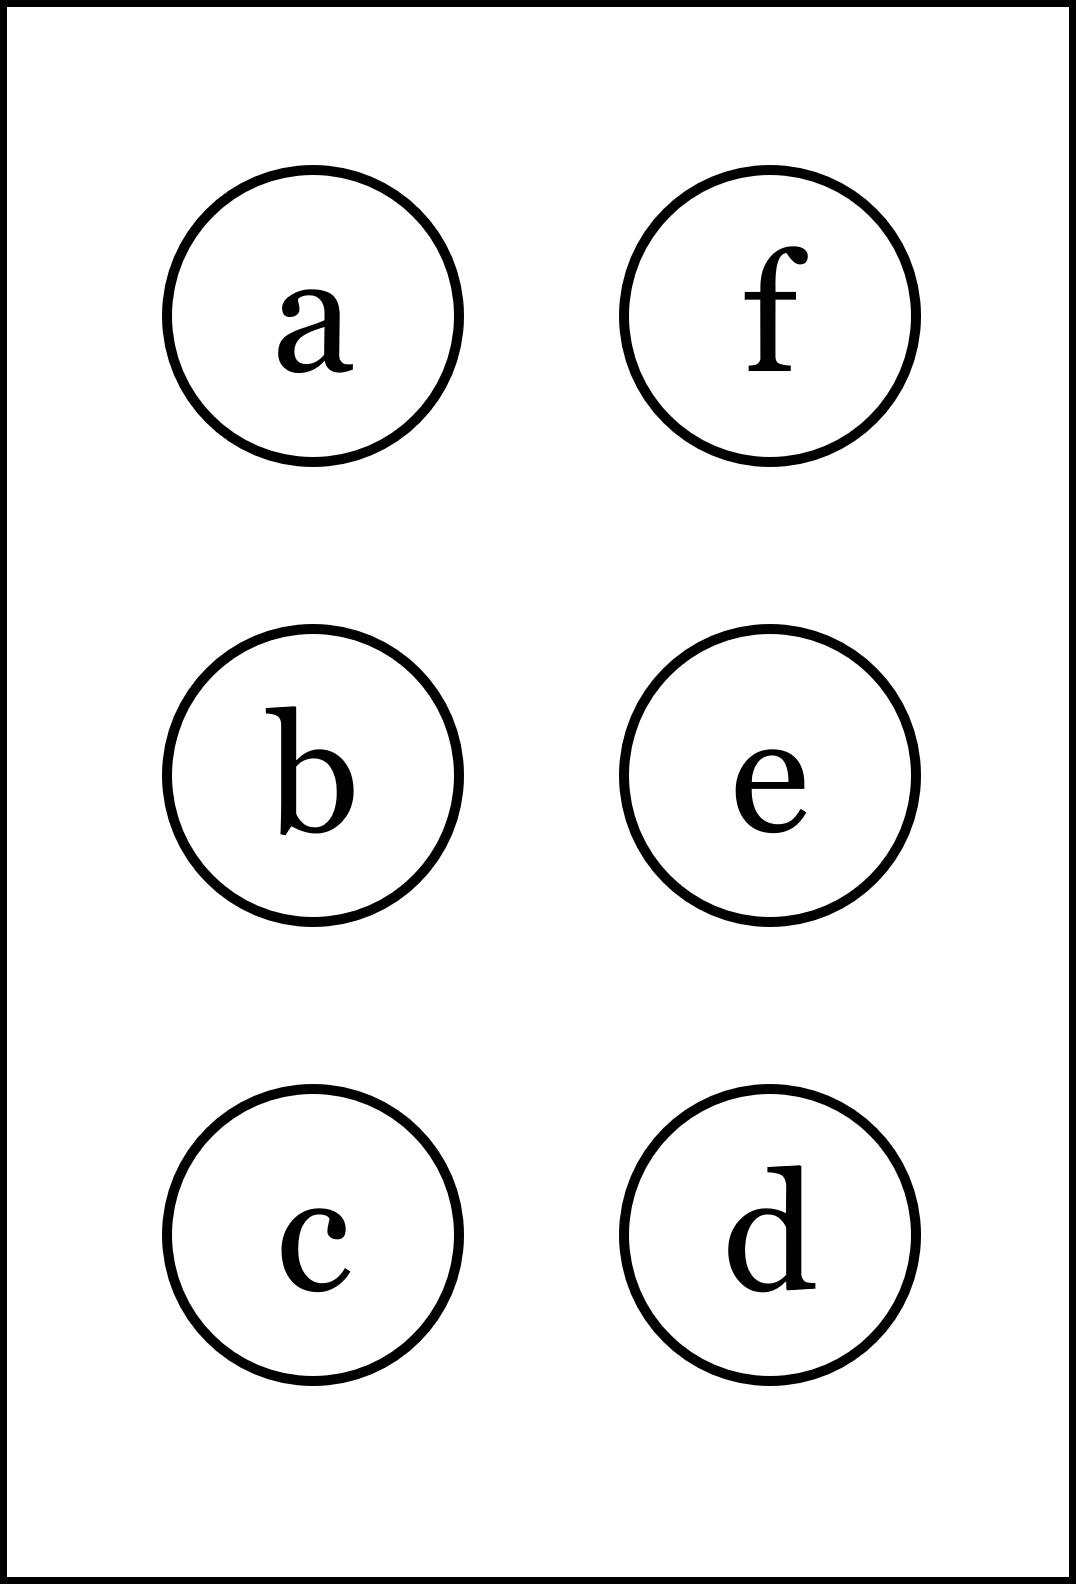
\includegraphics[height=40mm]{../images/braille.png}
{\small Písmeno Braillovej abecedy}
\end{center}
\end{minipage}
\end{center}
\end{minipage}
%
\end{tabular}
\newpage
\thispagestyle{empty}
\begin{tabular}{c:c}
\begin{minipage}[c][104.5mm][t]{0.5\linewidth}
\begin{center}
\vspace{7mm}
{\huge Kvadratická rovnice, skupina \textit{Lambda $\lambda$} -\romannumeral1}\\[5mm]
\textit{Jméno:}\phantom{xxxxxxxxxxxxxxxxxxxxxxxxxxxxxxxxxxxxxxxxxxxxxxxxxxxxxxxxxxxxxxxxx}\\[5mm]
\begin{minipage}{0.95\linewidth}
\begin{center}
V \textbf{(a)} a \textbf{(b)} zjisti počet řešení. V \textbf{(c)} x-ovú polohu vrcholu, a v \textbf{(d)} y-ovú polohu vrcholu.\\V \textbf{(e)} a \textbf{(f)} zjisti součet řešení. Pokud ti vyjde stejný výsledek jako je za otazníky, tak\\napravo obarvi příslušející kroužek načerno. \textbf{Spolu odevzdejte výsledné slovo}.
\end{center}
\end{minipage}
\\[1mm]
\begin{minipage}{0.79\linewidth}
\begin{center}
\begin{varwidth}{\linewidth}
\begin{enumerate}
\Large
\item $x^2-4x+1=0$\quad \dotfill\; ???\;\dotfill \quad 2
\item $2x^2+7x-4=0$\quad \dotfill\; ???\;\dotfill \quad 2
\item $f(x)=-x^2-3x+1$\quad \dotfill\; ???\;\dotfill \quad $\nicefrac{-3}{2}$
\item $f(x)=-7x^2+3x-8$\quad \dotfill\; ???\;\dotfill \quad $\nicefrac{-103}{28}$
\item $-2x^2+6x+20=0$\quad \dotfill\; ???\;\dotfill \quad 3
\item $-2x^2+x+21=0$\quad \dotfill\; ???\;\dotfill \quad $\nicefrac{-13}{2}$
\end{enumerate}
\end{varwidth}
\end{center}
\end{minipage}
\begin{minipage}{0.20\linewidth}
\begin{center}
{\Huge\bfseries 1.} \\[2mm]
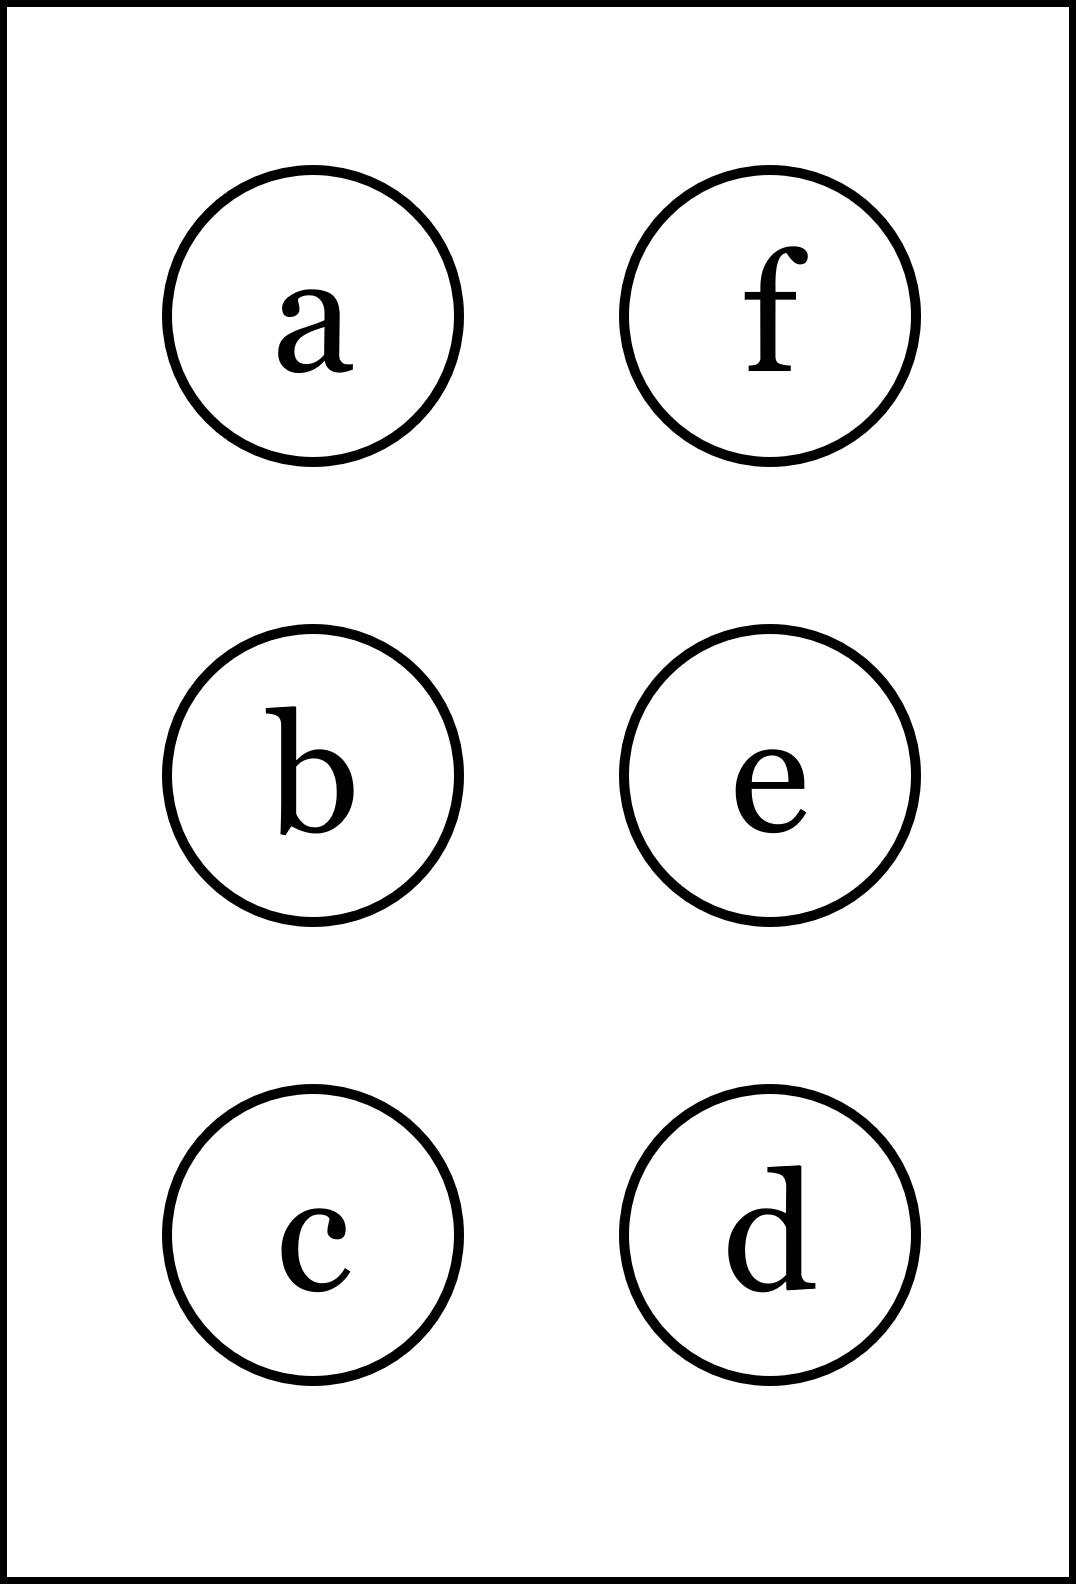
\includegraphics[height=40mm]{../images/braille.png}
{\small Písmeno Braillovej abecedy}
\end{center}
\end{minipage}
\end{center}
\end{minipage}
&
\begin{minipage}[c][104.5mm][t]{0.5\linewidth}
\begin{center}
\vspace{7mm}
{\huge Kvadratická rovnice, skupina \textit{Lambda $\lambda$} -\romannumeral2}\\[5mm]
\textit{Jméno:}\phantom{xxxxxxxxxxxxxxxxxxxxxxxxxxxxxxxxxxxxxxxxxxxxxxxxxxxxxxxxxxxxxxxxx}\\[5mm]
\begin{minipage}{0.95\linewidth}
\begin{center}
V \textbf{(a)} a \textbf{(b)} zjisti počet řešení. V \textbf{(c)} x-ovú polohu vrcholu, a v \textbf{(d)} y-ovú polohu vrcholu.\\V \textbf{(e)} a \textbf{(f)} zjisti součet řešení. Pokud ti vyjde stejný výsledek jako je za otazníky, tak\\napravo obarvi příslušející kroužek načerno. \textbf{Spolu odevzdejte výsledné slovo}.
\end{center}
\end{minipage}
\\[1mm]
\begin{minipage}{0.79\linewidth}
\begin{center}
\begin{varwidth}{\linewidth}
\begin{enumerate}
\Large
\item $-x^2-8x+8=0$\quad \dotfill\; ???\;\dotfill \quad 2
\item $-2x^2+3x-5=0$\quad \dotfill\; ???\;\dotfill \quad 2
\item $f(x)=-3x^2+6x+1$\quad \dotfill\; ???\;\dotfill \quad $1$
\item $f(x)=-x^2-9x-4$\quad \dotfill\; ???\;\dotfill \quad $\nicefrac{65}{4}$
\item $x^2-9x+20=0$\quad \dotfill\; ???\;\dotfill \quad 10
\item $-4x^2+6x+10=0$\quad \dotfill\; ???\;\dotfill \quad $\nicefrac{7}{2}$
\end{enumerate}
\end{varwidth}
\end{center}
\end{minipage}
\begin{minipage}{0.20\linewidth}
\begin{center}
{\Huge\bfseries 2.} \\[2mm]
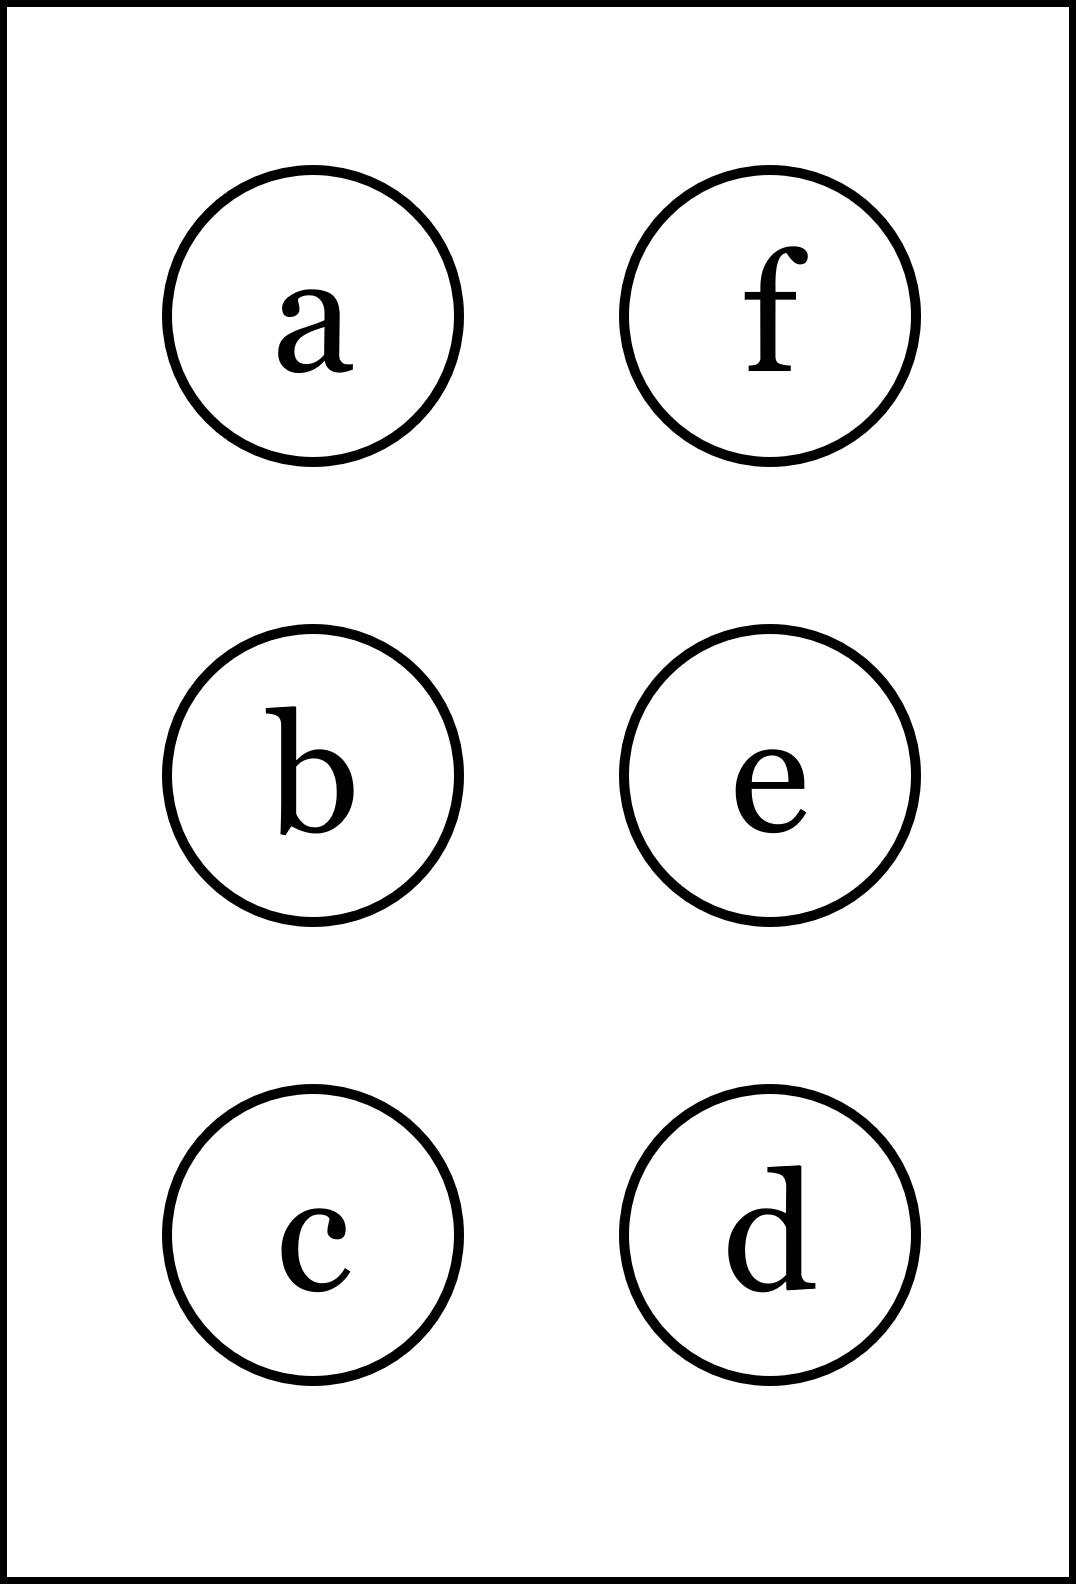
\includegraphics[height=40mm]{../images/braille.png}
{\small Písmeno Braillovej abecedy}
\end{center}
\end{minipage}
\end{center}
\end{minipage}
\\ \hdashline
\begin{minipage}[c][104.5mm][t]{0.5\linewidth}
\begin{center}
\vspace{7mm}
{\huge Kvadratická rovnice, skupina \textit{Lambda $\lambda$} -\romannumeral3}\\[5mm]
\textit{Jméno:}\phantom{xxxxxxxxxxxxxxxxxxxxxxxxxxxxxxxxxxxxxxxxxxxxxxxxxxxxxxxxxxxxxxxxx}\\[5mm]
\begin{minipage}{0.95\linewidth}
\begin{center}
V \textbf{(a)} a \textbf{(b)} zjisti počet řešení. V \textbf{(c)} x-ovú polohu vrcholu, a v \textbf{(d)} y-ovú polohu vrcholu.\\V \textbf{(e)} a \textbf{(f)} zjisti součet řešení. Pokud ti vyjde stejný výsledek jako je za otazníky, tak\\napravo obarvi příslušející kroužek načerno. \textbf{Spolu odevzdejte výsledné slovo}.
\end{center}
\end{minipage}
\\[1mm]
\begin{minipage}{0.79\linewidth}
\begin{center}
\begin{varwidth}{\linewidth}
\begin{enumerate}
\Large
\item $9x^2-3x+1=0$\quad \dotfill\; ???\;\dotfill \quad 0
\item $4x^2+x-2=0$\quad \dotfill\; ???\;\dotfill \quad 0
\item $f(x)=x^2+7x+3$\quad \dotfill\; ???\;\dotfill \quad $\nicefrac{-7}{2}$
\item $f(x)=-6x^2+2x+4$\quad \dotfill\; ???\;\dotfill \quad $\nicefrac{13}{6}$
\item $-2x^2+14x-24=0$\quad \dotfill\; ???\;\dotfill \quad 10
\item $-4x^2+12x-8=0$\quad \dotfill\; ???\;\dotfill \quad $1$
\end{enumerate}
\end{varwidth}
\end{center}
\end{minipage}
\begin{minipage}{0.20\linewidth}
\begin{center}
{\Huge\bfseries 3.} \\[2mm]
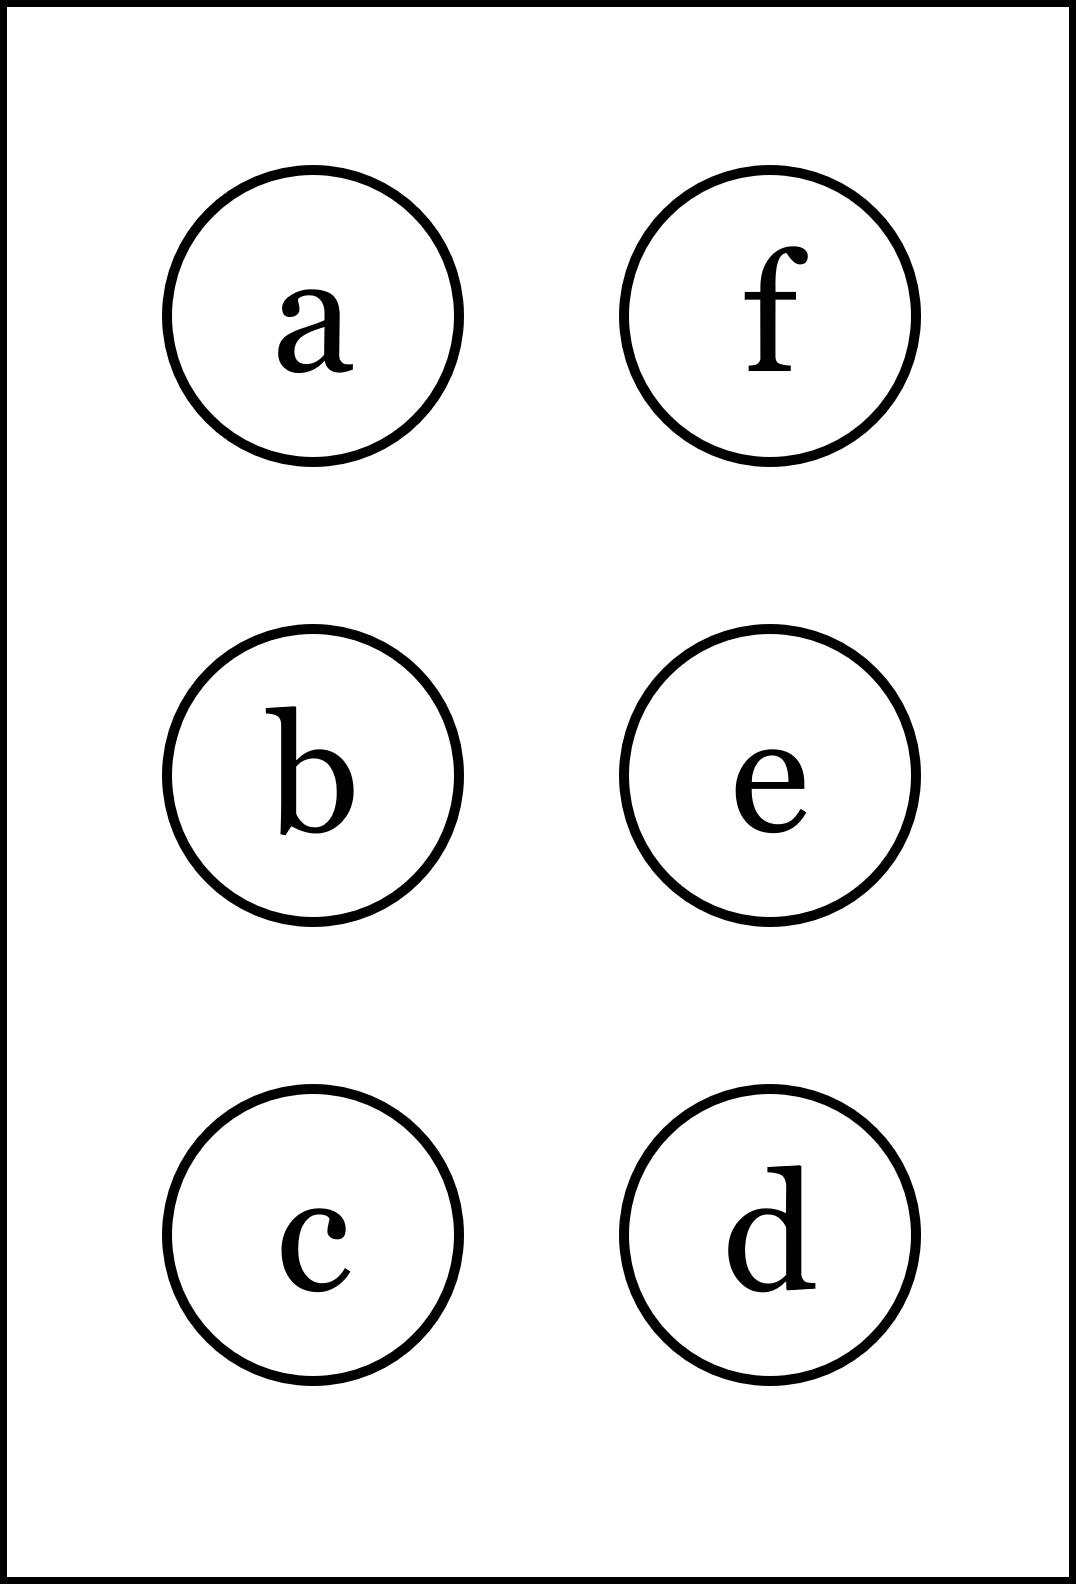
\includegraphics[height=40mm]{../images/braille.png}
{\small Písmeno Braillovej abecedy}
\end{center}
\end{minipage}
\end{center}
\end{minipage}
&
\begin{minipage}[c][104.5mm][t]{0.5\linewidth}
\begin{center}
\vspace{7mm}
{\huge Kvadratická rovnice, skupina \textit{Lambda $\lambda$} -\romannumeral4}\\[5mm]
\textit{Jméno:}\phantom{xxxxxxxxxxxxxxxxxxxxxxxxxxxxxxxxxxxxxxxxxxxxxxxxxxxxxxxxxxxxxxxxx}\\[5mm]
\begin{minipage}{0.95\linewidth}
\begin{center}
V \textbf{(a)} a \textbf{(b)} zjisti počet řešení. V \textbf{(c)} x-ovú polohu vrcholu, a v \textbf{(d)} y-ovú polohu vrcholu.\\V \textbf{(e)} a \textbf{(f)} zjisti součet řešení. Pokud ti vyjde stejný výsledek jako je za otazníky, tak\\napravo obarvi příslušející kroužek načerno. \textbf{Spolu odevzdejte výsledné slovo}.
\end{center}
\end{minipage}
\\[1mm]
\begin{minipage}{0.79\linewidth}
\begin{center}
\begin{varwidth}{\linewidth}
\begin{enumerate}
\Large
\item $2x^2+5x+5=0$\quad \dotfill\; ???\;\dotfill \quad 0
\item $-2x^2+4x+1=0$\quad \dotfill\; ???\;\dotfill \quad 0
\item $f(x)=-4x^2+6x-3$\quad \dotfill\; ???\;\dotfill \quad $\nicefrac{-3}{4}$
\item $f(x)=5x^2+2x+5$\quad \dotfill\; ???\;\dotfill \quad $\nicefrac{23}{10}$
\item $x^2+12x+35=0$\quad \dotfill\; ???\;\dotfill \quad -14
\item $-6x^2+x+5=0$\quad \dotfill\; ???\;\dotfill \quad $\nicefrac{-11}{6}$
\end{enumerate}
\end{varwidth}
\end{center}
\end{minipage}
\begin{minipage}{0.20\linewidth}
\begin{center}
{\Huge\bfseries 4.} \\[2mm]
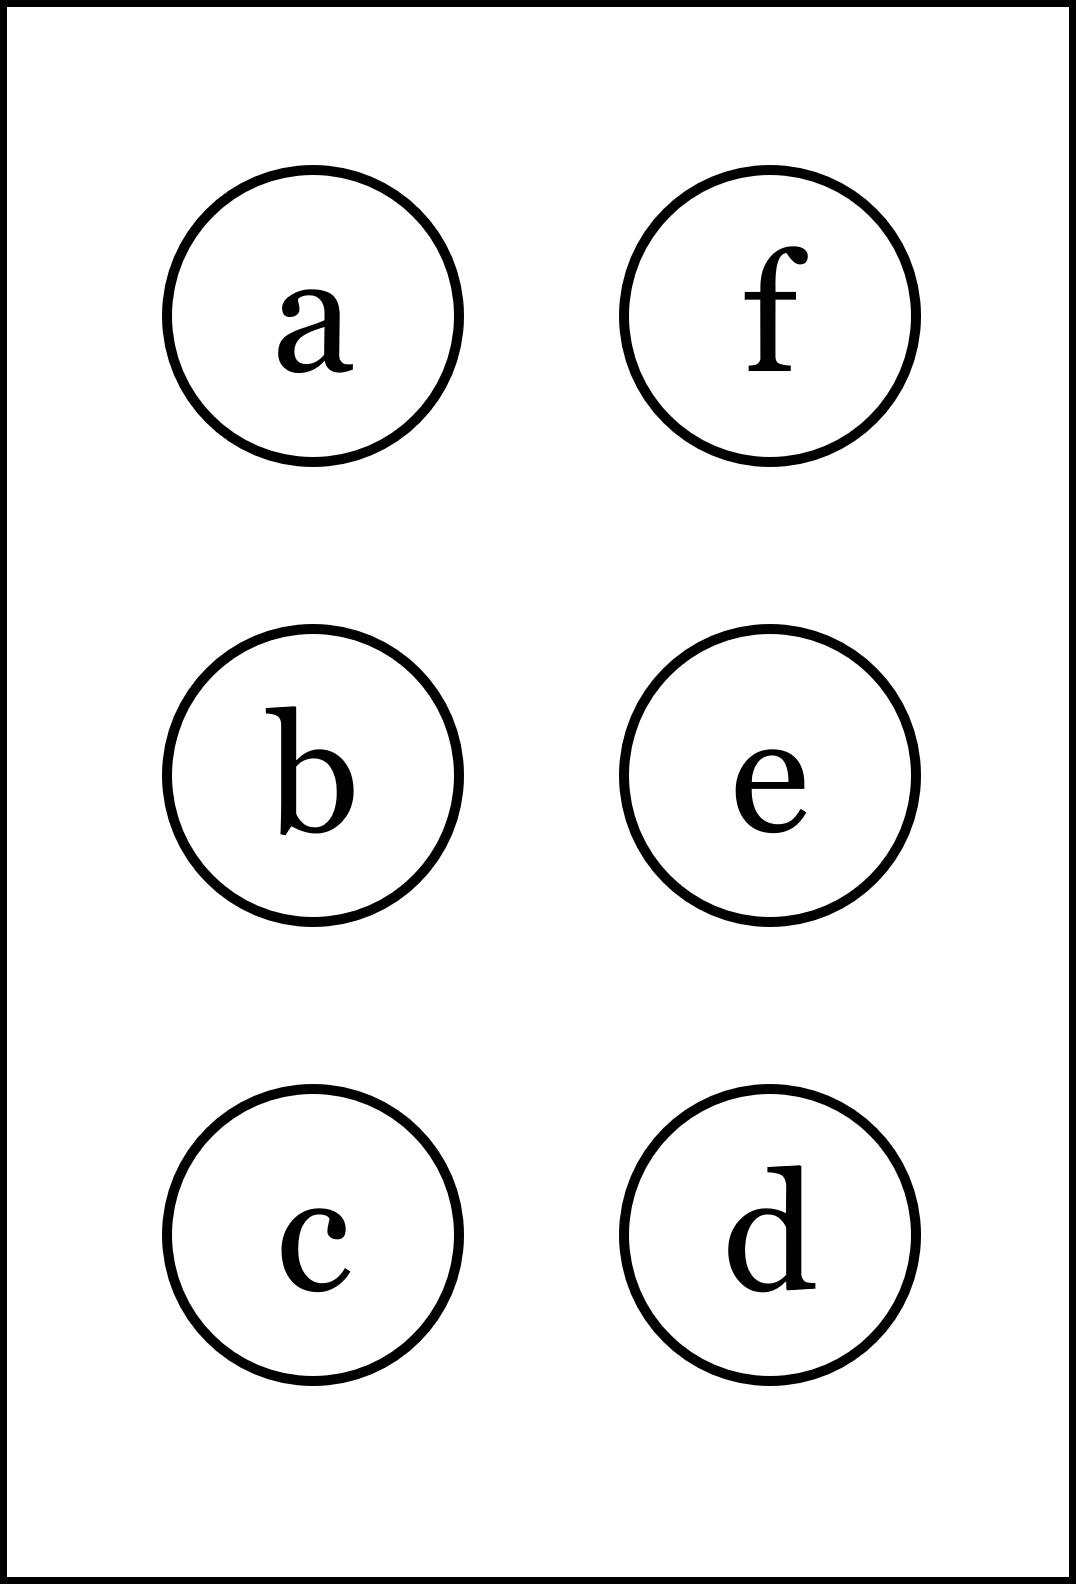
\includegraphics[height=40mm]{../images/braille.png}
{\small Písmeno Braillovej abecedy}
\end{center}
\end{minipage}
\end{center}
\end{minipage}
%
\end{tabular}
\newpage
\thispagestyle{empty}
\begin{tabular}{c:c}
\begin{minipage}[c][104.5mm][t]{0.5\linewidth}
\begin{center}
\vspace{7mm}
{\huge Kvadratická rovnice, skupina \textit{Mu $\mu$} -\romannumeral1}\\[5mm]
\textit{Jméno:}\phantom{xxxxxxxxxxxxxxxxxxxxxxxxxxxxxxxxxxxxxxxxxxxxxxxxxxxxxxxxxxxxxxxxx}\\[5mm]
\begin{minipage}{0.95\linewidth}
\begin{center}
V \textbf{(a)} a \textbf{(b)} zjisti počet řešení. V \textbf{(c)} x-ovú polohu vrcholu, a v \textbf{(d)} y-ovú polohu vrcholu.\\V \textbf{(e)} a \textbf{(f)} zjisti součet řešení. Pokud ti vyjde stejný výsledek jako je za otazníky, tak\\napravo obarvi příslušející kroužek načerno. \textbf{Spolu odevzdejte výsledné slovo}.
\end{center}
\end{minipage}
\\[1mm]
\begin{minipage}{0.79\linewidth}
\begin{center}
\begin{varwidth}{\linewidth}
\begin{enumerate}
\Large
\item $x^2+4x-5=0$\quad \dotfill\; ???\;\dotfill \quad 2
\item $-8x^2-3x+5=0$\quad \dotfill\; ???\;\dotfill \quad 2
\item $f(x)=7x^2-9x+2$\quad \dotfill\; ???\;\dotfill \quad $\nicefrac{-9}{14}$
\item $f(x)=-2x^2-x+6$\quad \dotfill\; ???\;\dotfill \quad $\nicefrac{25}{8}$
\item $-2x^2-10x-12=0$\quad \dotfill\; ???\;\dotfill \quad -6
\item $10x^2-14x+4=0$\quad \dotfill\; ???\;\dotfill \quad $\nicefrac{7}{5}$
\end{enumerate}
\end{varwidth}
\end{center}
\end{minipage}
\begin{minipage}{0.20\linewidth}
\begin{center}
{\Huge\bfseries 1.} \\[2mm]
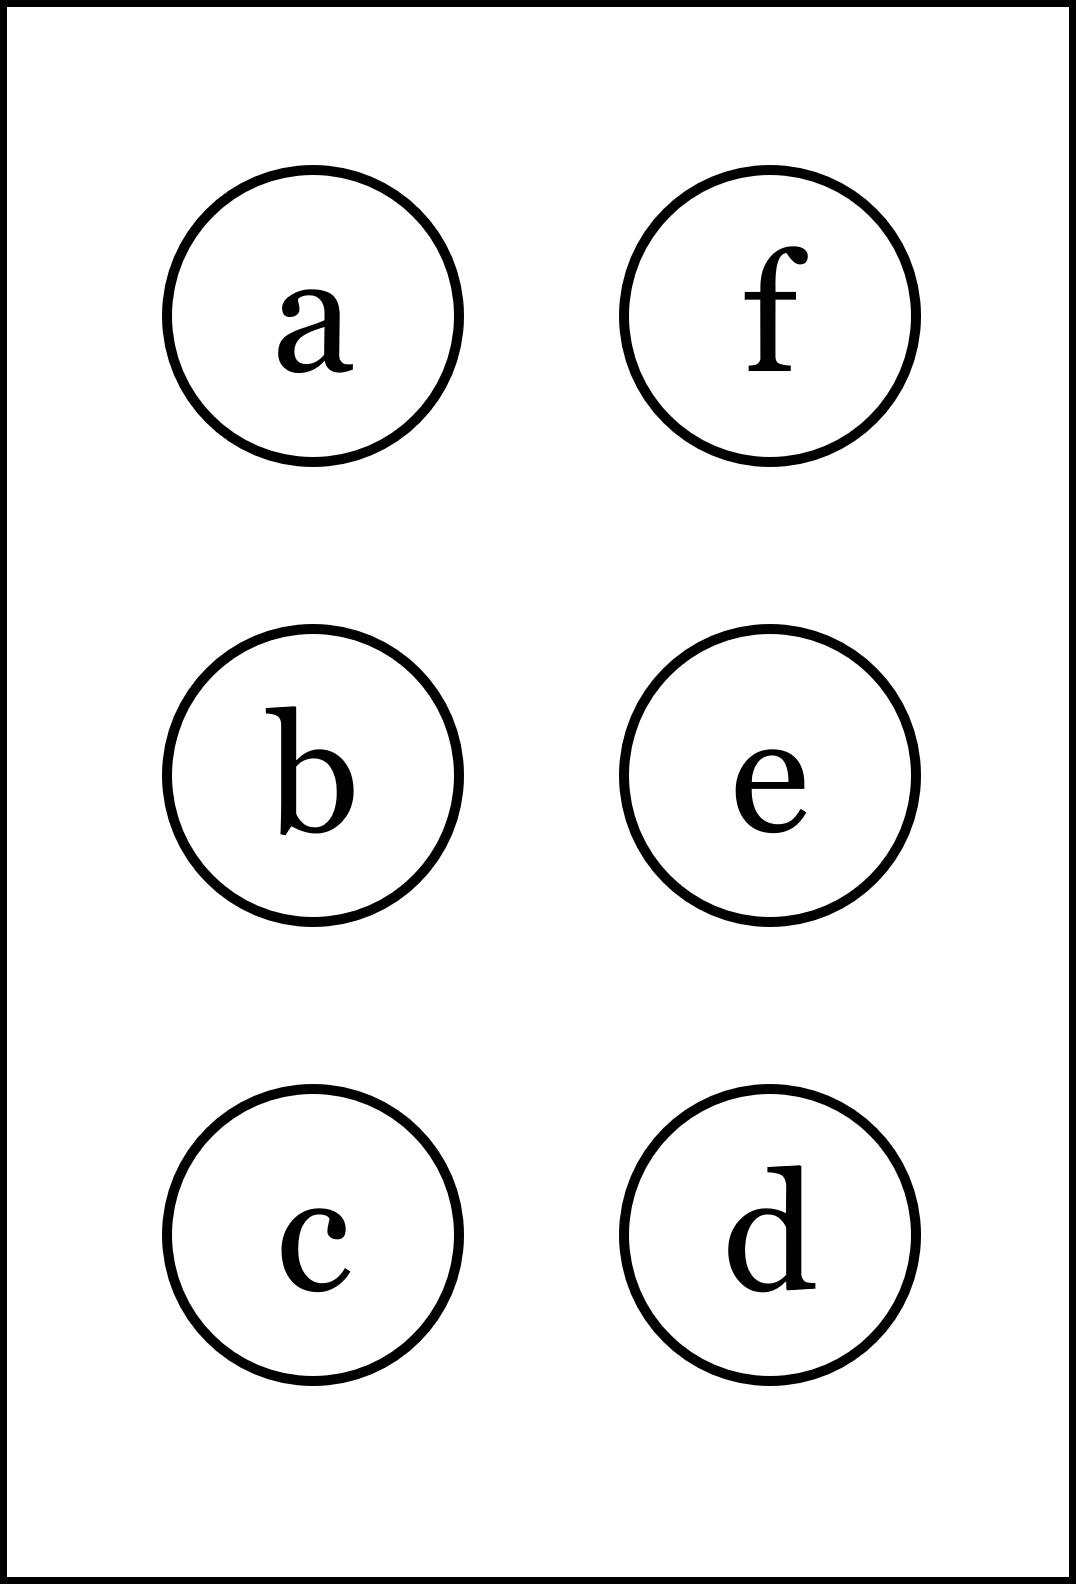
\includegraphics[height=40mm]{../images/braille.png}
{\small Písmeno Braillovej abecedy}
\end{center}
\end{minipage}
\end{center}
\end{minipage}
&
\begin{minipage}[c][104.5mm][t]{0.5\linewidth}
\begin{center}
\vspace{7mm}
{\huge Kvadratická rovnice, skupina \textit{Mu $\mu$} -\romannumeral2}\\[5mm]
\textit{Jméno:}\phantom{xxxxxxxxxxxxxxxxxxxxxxxxxxxxxxxxxxxxxxxxxxxxxxxxxxxxxxxxxxxxxxxxx}\\[5mm]
\begin{minipage}{0.95\linewidth}
\begin{center}
V \textbf{(a)} a \textbf{(b)} zjisti počet řešení. V \textbf{(c)} x-ovú polohu vrcholu, a v \textbf{(d)} y-ovú polohu vrcholu.\\V \textbf{(e)} a \textbf{(f)} zjisti součet řešení. Pokud ti vyjde stejný výsledek jako je za otazníky, tak\\napravo obarvi příslušející kroužek načerno. \textbf{Spolu odevzdejte výsledné slovo}.
\end{center}
\end{minipage}
\\[1mm]
\begin{minipage}{0.79\linewidth}
\begin{center}
\begin{varwidth}{\linewidth}
\begin{enumerate}
\Large
\item $-5x^2+4x-4=0$\quad \dotfill\; ???\;\dotfill \quad 0
\item $5x^2+7x-2=0$\quad \dotfill\; ???\;\dotfill \quad 2
\item $f(x)=5x^2+7x+6$\quad \dotfill\; ???\;\dotfill \quad $\nicefrac{-7}{10}$
\item $f(x)=9x^2+2x+4$\quad \dotfill\; ???\;\dotfill \quad $\nicefrac{17}{9}$
\item $-2x^2+16x-24=0$\quad \dotfill\; ???\;\dotfill \quad 5
\item $4x^2-6x+2=0$\quad \dotfill\; ???\;\dotfill \quad $\nicefrac{1}{2}$
\end{enumerate}
\end{varwidth}
\end{center}
\end{minipage}
\begin{minipage}{0.20\linewidth}
\begin{center}
{\Huge\bfseries 2.} \\[2mm]
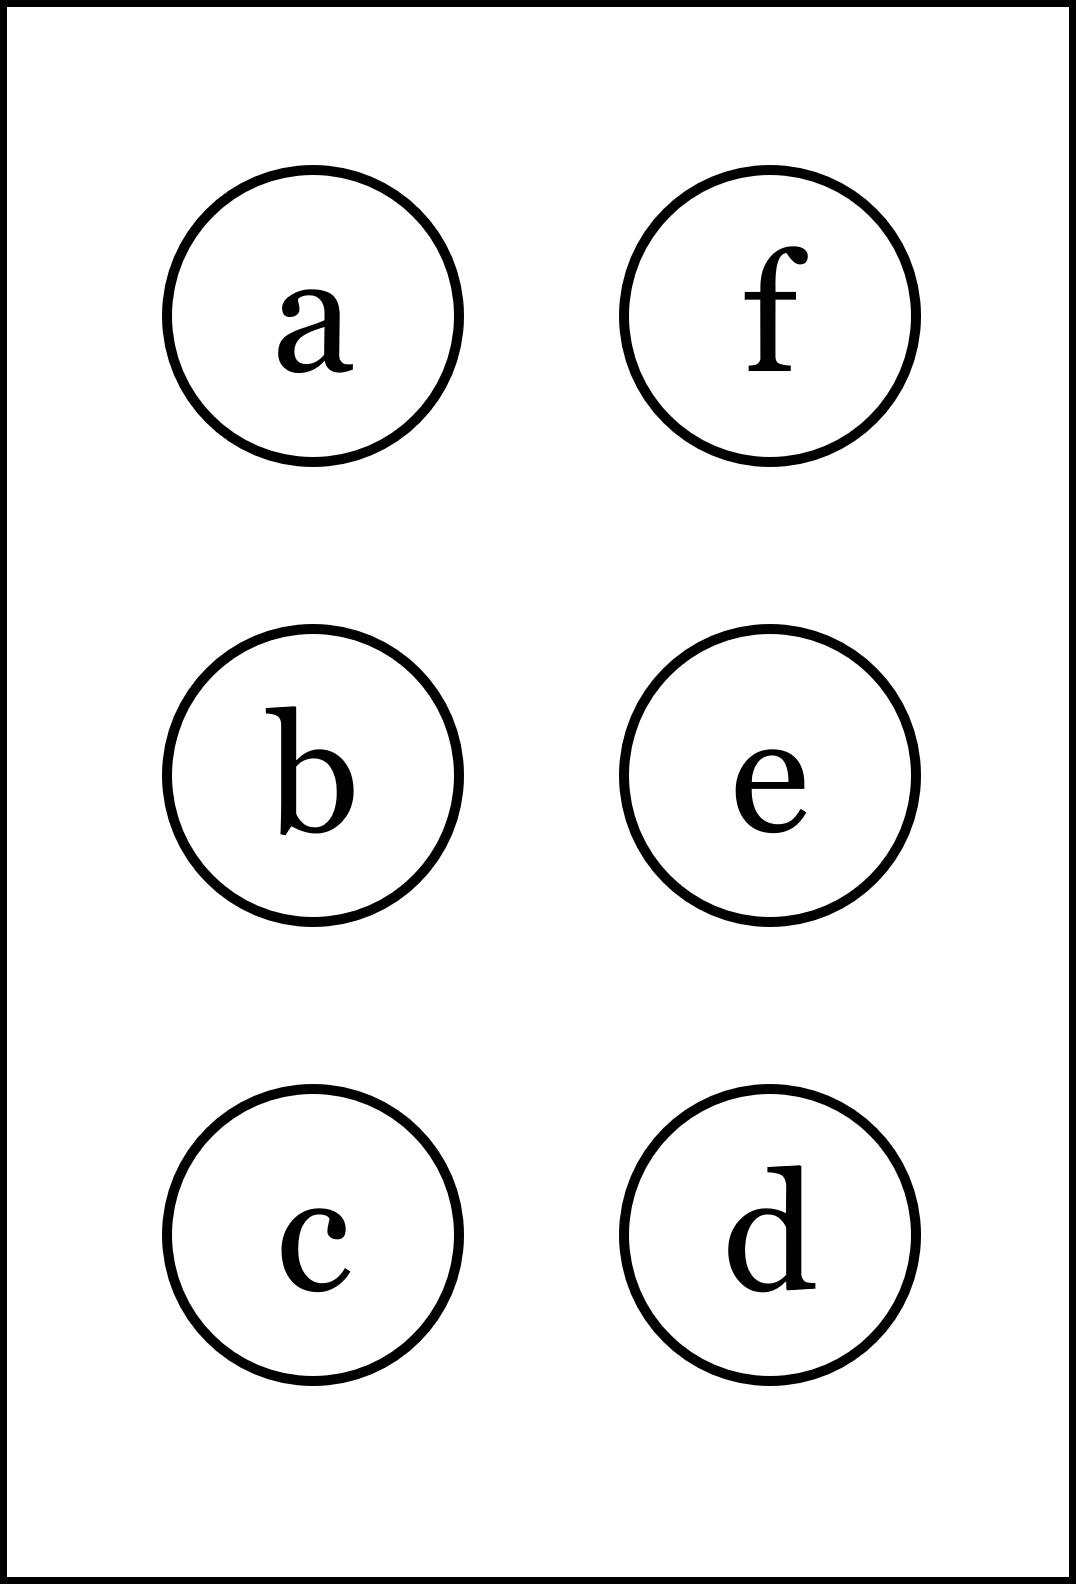
\includegraphics[height=40mm]{../images/braille.png}
{\small Písmeno Braillovej abecedy}
\end{center}
\end{minipage}
\end{center}
\end{minipage}
\\ \hdashline
\begin{minipage}[c][104.5mm][t]{0.5\linewidth}
\begin{center}
\vspace{7mm}
{\huge Kvadratická rovnice, skupina \textit{Mu $\mu$} -\romannumeral3}\\[5mm]
\textit{Jméno:}\phantom{xxxxxxxxxxxxxxxxxxxxxxxxxxxxxxxxxxxxxxxxxxxxxxxxxxxxxxxxxxxxxxxxx}\\[5mm]
\begin{minipage}{0.95\linewidth}
\begin{center}
V \textbf{(a)} a \textbf{(b)} zjisti počet řešení. V \textbf{(c)} x-ovú polohu vrcholu, a v \textbf{(d)} y-ovú polohu vrcholu.\\V \textbf{(e)} a \textbf{(f)} zjisti součet řešení. Pokud ti vyjde stejný výsledek jako je za otazníky, tak\\napravo obarvi příslušející kroužek načerno. \textbf{Spolu odevzdejte výsledné slovo}.
\end{center}
\end{minipage}
\\[1mm]
\begin{minipage}{0.79\linewidth}
\begin{center}
\begin{varwidth}{\linewidth}
\begin{enumerate}
\Large
\item $-6x^2+4x-6=0$\quad \dotfill\; ???\;\dotfill \quad 0
\item $-8x^2+7x-7=0$\quad \dotfill\; ???\;\dotfill \quad 1
\item $f(x)=-2x^2-3x-7$\quad \dotfill\; ???\;\dotfill \quad $\nicefrac{3}{4}$
\item $f(x)=2x^2-x+7$\quad \dotfill\; ???\;\dotfill \quad $\nicefrac{27}{8}$
\item $-3x^2-9x+30=0$\quad \dotfill\; ???\;\dotfill \quad -3
\item $x^2+6x+8=0$\quad \dotfill\; ???\;\dotfill \quad $-2$
\end{enumerate}
\end{varwidth}
\end{center}
\end{minipage}
\begin{minipage}{0.20\linewidth}
\begin{center}
{\Huge\bfseries 3.} \\[2mm]
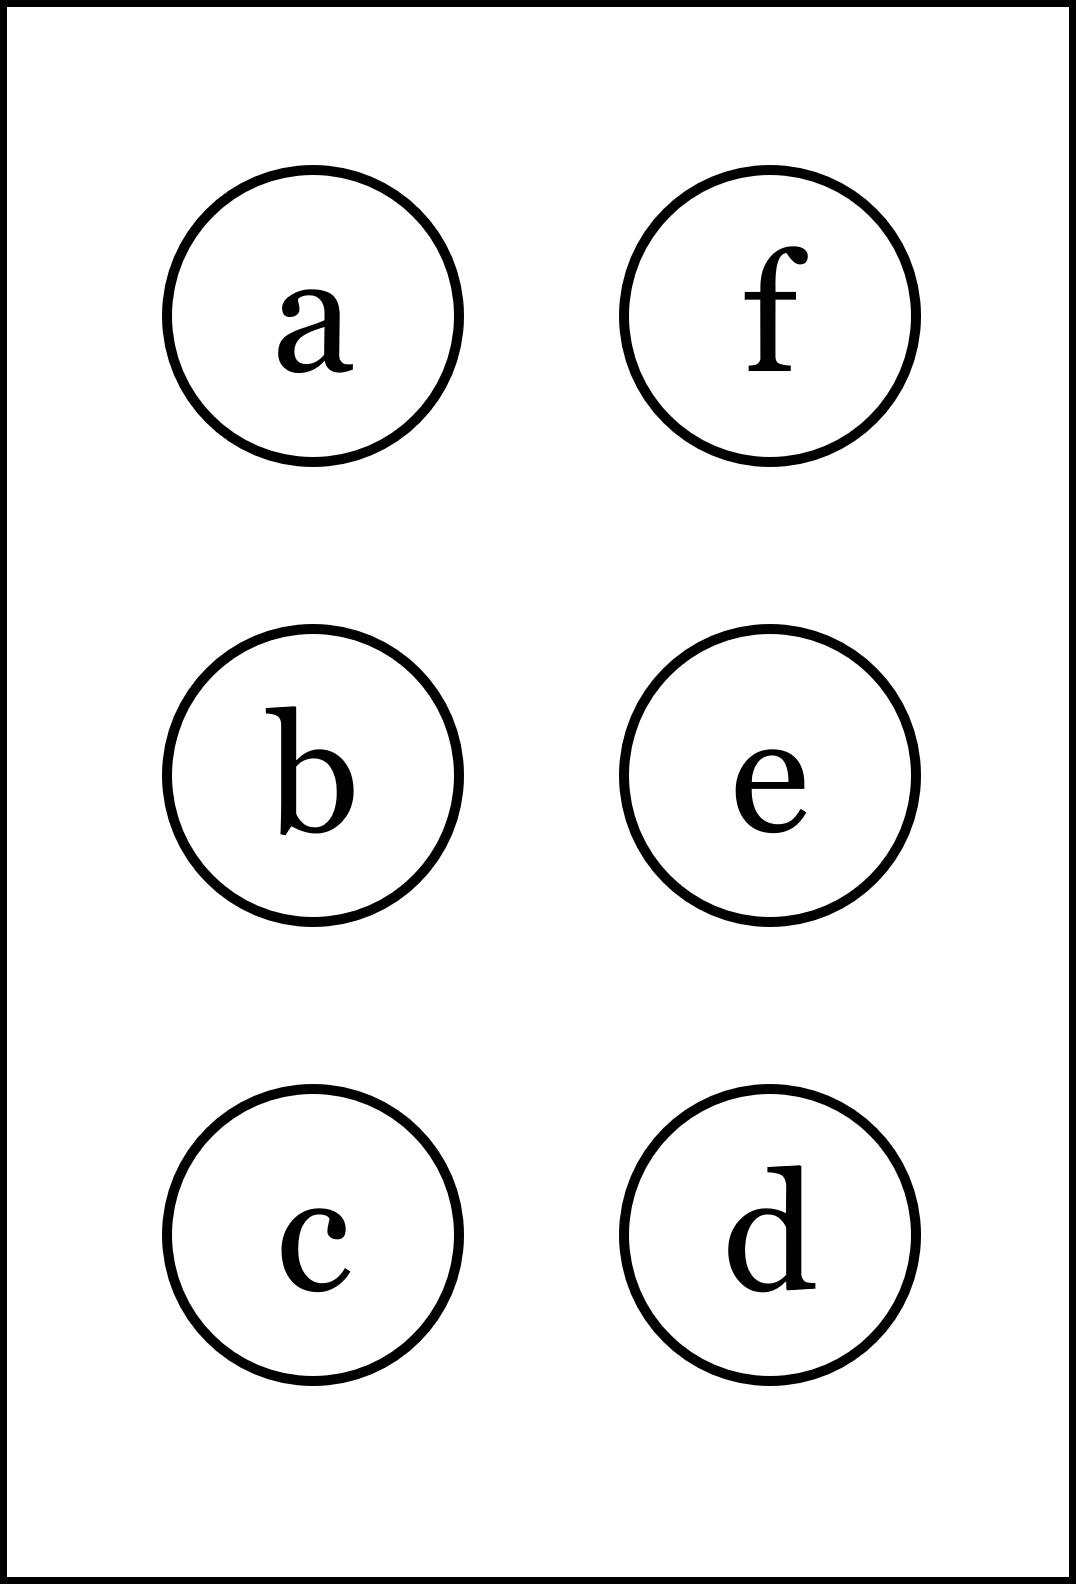
\includegraphics[height=40mm]{../images/braille.png}
{\small Písmeno Braillovej abecedy}
\end{center}
\end{minipage}
\end{center}
\end{minipage}
&
\begin{minipage}[c][104.5mm][t]{0.5\linewidth}
\begin{center}
\vspace{7mm}
{\huge Kvadratická rovnice, skupina \textit{Mu $\mu$} -\romannumeral4}\\[5mm]
\textit{Jméno:}\phantom{xxxxxxxxxxxxxxxxxxxxxxxxxxxxxxxxxxxxxxxxxxxxxxxxxxxxxxxxxxxxxxxxx}\\[5mm]
\begin{minipage}{0.95\linewidth}
\begin{center}
V \textbf{(a)} a \textbf{(b)} zjisti počet řešení. V \textbf{(c)} x-ovú polohu vrcholu, a v \textbf{(d)} y-ovú polohu vrcholu.\\V \textbf{(e)} a \textbf{(f)} zjisti součet řešení. Pokud ti vyjde stejný výsledek jako je za otazníky, tak\\napravo obarvi příslušející kroužek načerno. \textbf{Spolu odevzdejte výsledné slovo}.
\end{center}
\end{minipage}
\\[1mm]
\begin{minipage}{0.79\linewidth}
\begin{center}
\begin{varwidth}{\linewidth}
\begin{enumerate}
\Large
\item $-7x^2-5x+3=0$\quad \dotfill\; ???\;\dotfill \quad 2
\item $-x^2-x-3=0$\quad \dotfill\; ???\;\dotfill \quad 1
\item $f(x)=3x^2-x+2$\quad \dotfill\; ???\;\dotfill \quad $\nicefrac{1}{6}$
\item $f(x)=-2x^2-4x+4$\quad \dotfill\; ???\;\dotfill \quad $4$
\item $-x^2+4x+5=0$\quad \dotfill\; ???\;\dotfill \quad 1
\item $9x^2-6x-3=0$\quad \dotfill\; ???\;\dotfill \quad $\nicefrac{4}{3}$
\end{enumerate}
\end{varwidth}
\end{center}
\end{minipage}
\begin{minipage}{0.20\linewidth}
\begin{center}
{\Huge\bfseries 4.} \\[2mm]
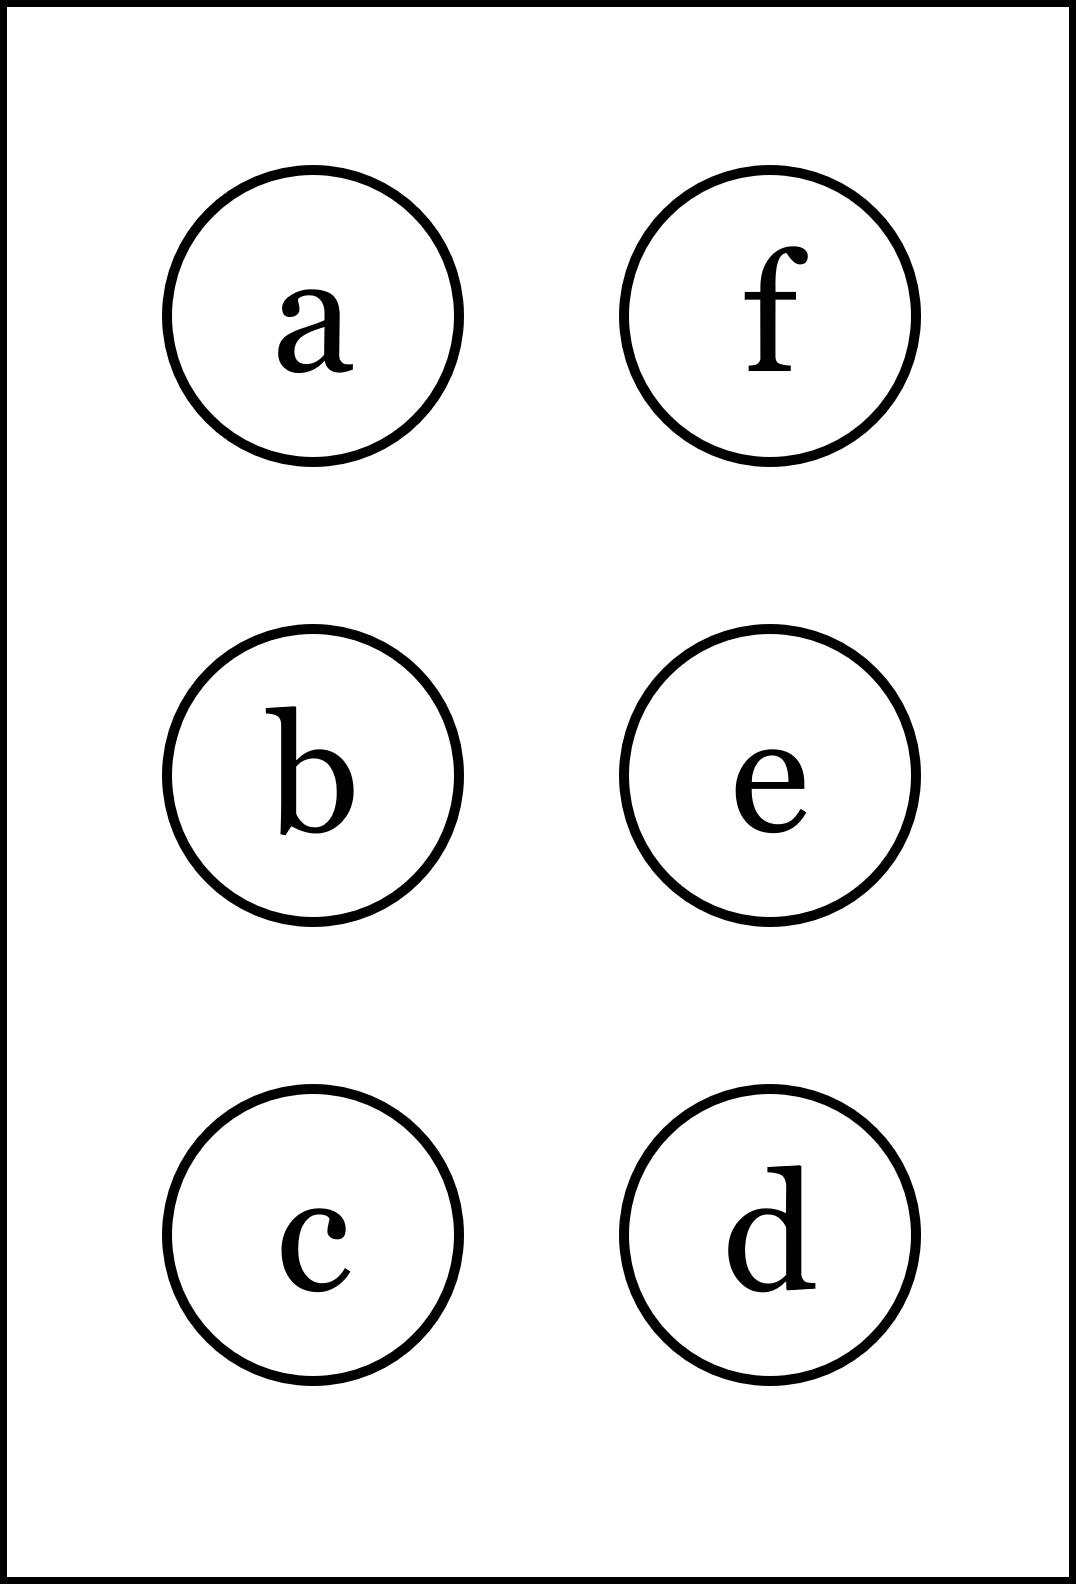
\includegraphics[height=40mm]{../images/braille.png}
{\small Písmeno Braillovej abecedy}
\end{center}
\end{minipage}
\end{center}
\end{minipage}
%
\end{tabular}
\newpage
\thispagestyle{empty}
\begin{tabular}{c:c}
\begin{minipage}[c][104.5mm][t]{0.5\linewidth}
\begin{center}
\vspace{7mm}
{\huge Kvadratická rovnice, skupina \textit{Nu $\nu$} -\romannumeral1}\\[5mm]
\textit{Jméno:}\phantom{xxxxxxxxxxxxxxxxxxxxxxxxxxxxxxxxxxxxxxxxxxxxxxxxxxxxxxxxxxxxxxxxx}\\[5mm]
\begin{minipage}{0.95\linewidth}
\begin{center}
V \textbf{(a)} a \textbf{(b)} zjisti počet řešení. V \textbf{(c)} x-ovú polohu vrcholu, a v \textbf{(d)} y-ovú polohu vrcholu.\\V \textbf{(e)} a \textbf{(f)} zjisti součet řešení. Pokud ti vyjde stejný výsledek jako je za otazníky, tak\\napravo obarvi příslušející kroužek načerno. \textbf{Spolu odevzdejte výsledné slovo}.
\end{center}
\end{minipage}
\\[1mm]
\begin{minipage}{0.79\linewidth}
\begin{center}
\begin{varwidth}{\linewidth}
\begin{enumerate}
\Large
\item $-x^2-x+1=0$\quad \dotfill\; ???\;\dotfill \quad 2
\item $2x^2+5x+8=0$\quad \dotfill\; ???\;\dotfill \quad 1
\item $f(x)=-x^2-5x+7$\quad \dotfill\; ???\;\dotfill \quad $\nicefrac{5}{2}$
\item $f(x)=6x^2+x+5$\quad \dotfill\; ???\;\dotfill \quad $\nicefrac{59}{24}$
\item $4x^2-4x-48=0$\quad \dotfill\; ???\;\dotfill \quad 1
\item $2x^2-12x+10=0$\quad \dotfill\; ???\;\dotfill \quad $-4$
\end{enumerate}
\end{varwidth}
\end{center}
\end{minipage}
\begin{minipage}{0.20\linewidth}
\begin{center}
{\Huge\bfseries 1.} \\[2mm]
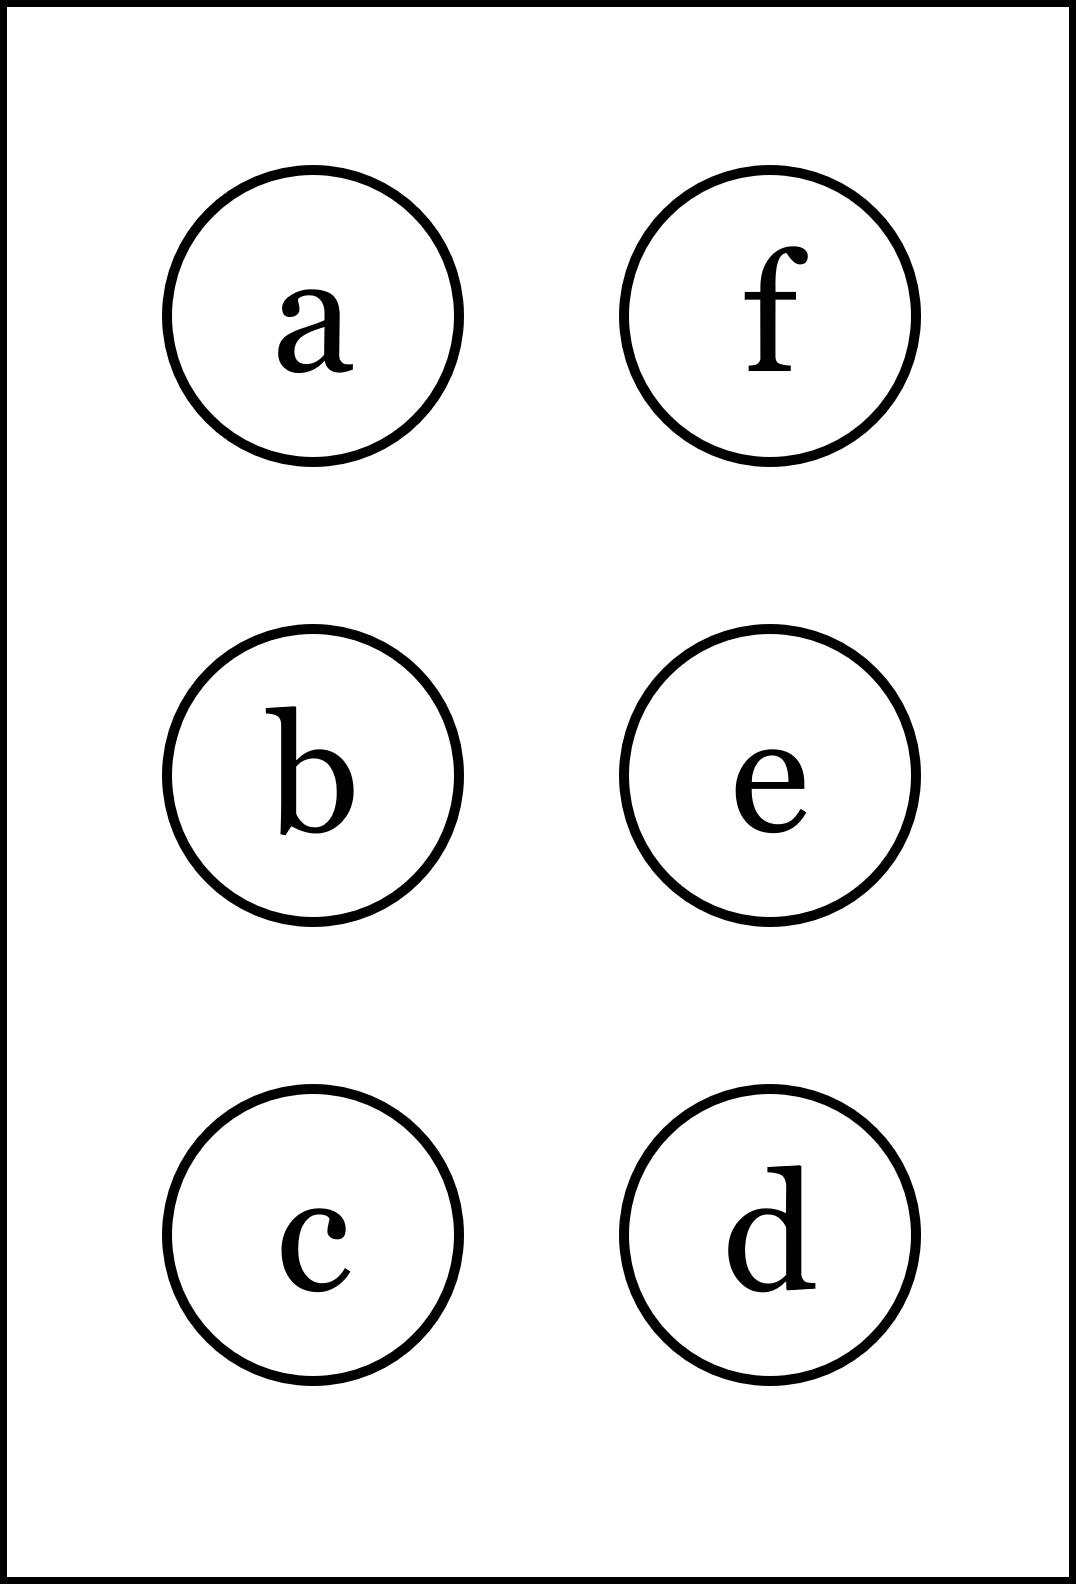
\includegraphics[height=40mm]{../images/braille.png}
{\small Písmeno Braillovej abecedy}
\end{center}
\end{minipage}
\end{center}
\end{minipage}
&
\begin{minipage}[c][104.5mm][t]{0.5\linewidth}
\begin{center}
\vspace{7mm}
{\huge Kvadratická rovnice, skupina \textit{Nu $\nu$} -\romannumeral2}\\[5mm]
\textit{Jméno:}\phantom{xxxxxxxxxxxxxxxxxxxxxxxxxxxxxxxxxxxxxxxxxxxxxxxxxxxxxxxxxxxxxxxxx}\\[5mm]
\begin{minipage}{0.95\linewidth}
\begin{center}
V \textbf{(a)} a \textbf{(b)} zjisti počet řešení. V \textbf{(c)} x-ovú polohu vrcholu, a v \textbf{(d)} y-ovú polohu vrcholu.\\V \textbf{(e)} a \textbf{(f)} zjisti součet řešení. Pokud ti vyjde stejný výsledek jako je za otazníky, tak\\napravo obarvi příslušející kroužek načerno. \textbf{Spolu odevzdejte výsledné slovo}.
\end{center}
\end{minipage}
\\[1mm]
\begin{minipage}{0.79\linewidth}
\begin{center}
\begin{varwidth}{\linewidth}
\begin{enumerate}
\Large
\item $-x^2-5x-2=0$\quad \dotfill\; ???\;\dotfill \quad 2
\item $-x^2-3x+4=0$\quad \dotfill\; ???\;\dotfill \quad 0
\item $f(x)=-8x^2-3x-2$\quad \dotfill\; ???\;\dotfill \quad $\nicefrac{-3}{16}$
\item $f(x)=4x^2+9x-4$\quad \dotfill\; ???\;\dotfill \quad $\nicefrac{-113}{16}$
\item $x^2+4x-12=0$\quad \dotfill\; ???\;\dotfill \quad -3
\item $-6x^2+2x+8=0$\quad \dotfill\; ???\;\dotfill \quad $\nicefrac{1}{3}$
\end{enumerate}
\end{varwidth}
\end{center}
\end{minipage}
\begin{minipage}{0.20\linewidth}
\begin{center}
{\Huge\bfseries 2.} \\[2mm]
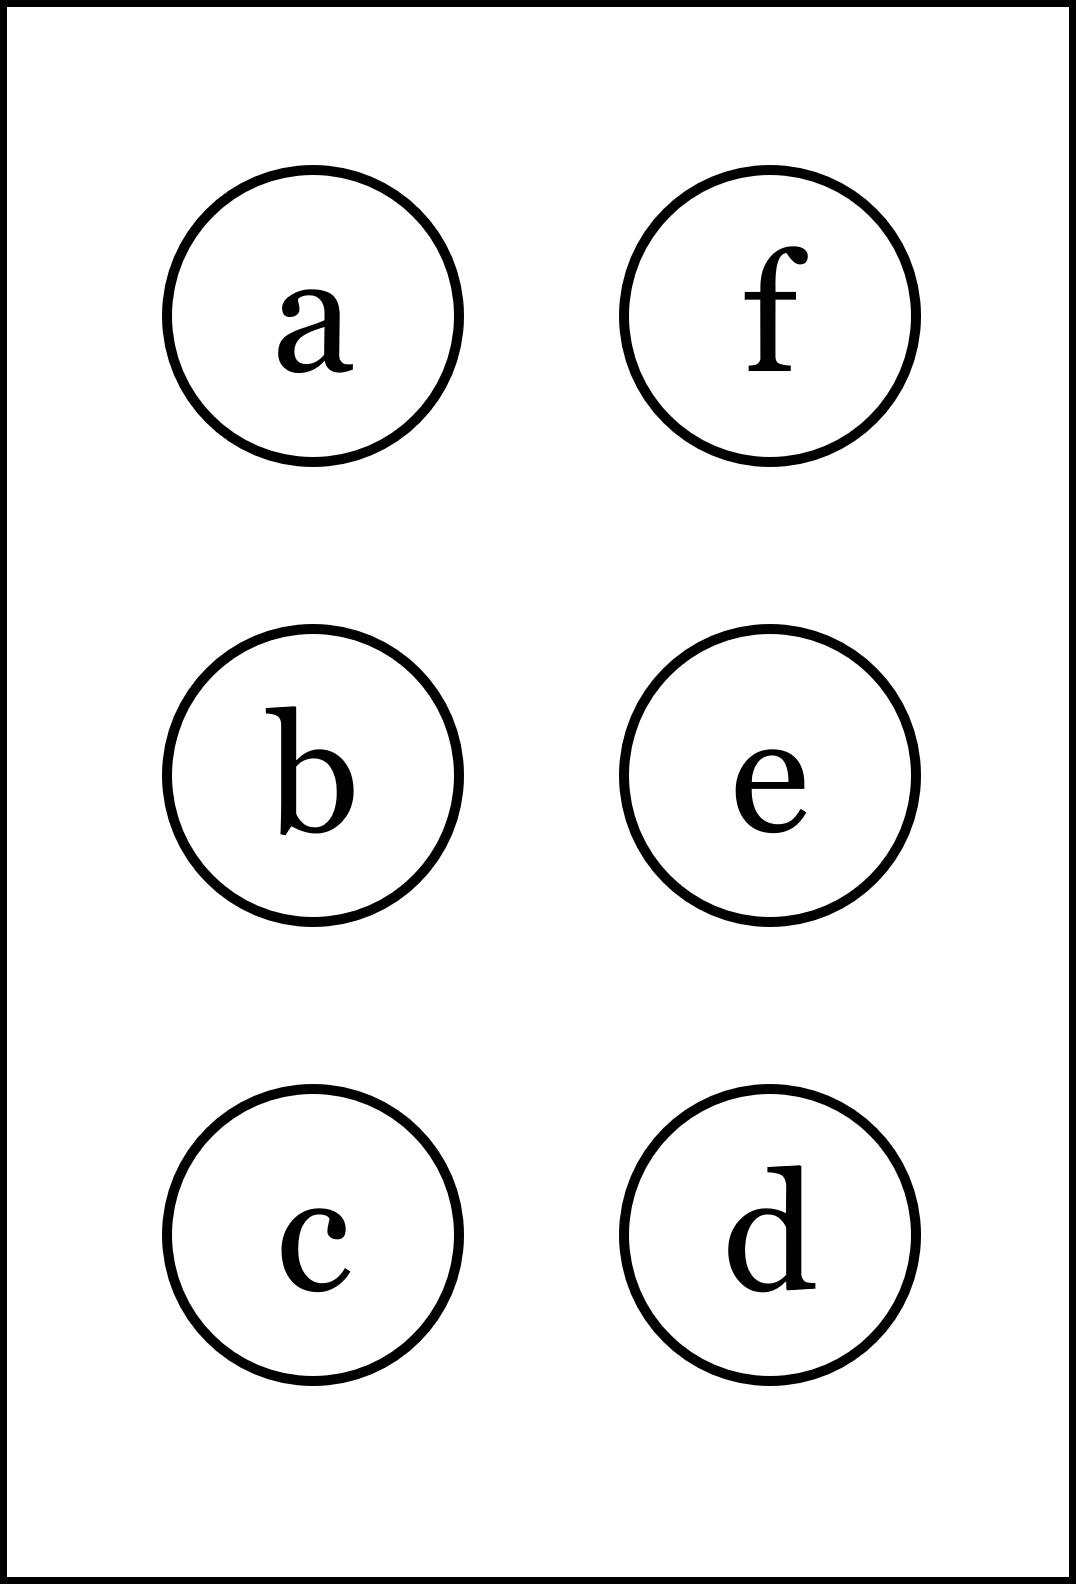
\includegraphics[height=40mm]{../images/braille.png}
{\small Písmeno Braillovej abecedy}
\end{center}
\end{minipage}
\end{center}
\end{minipage}
\\ \hdashline
\begin{minipage}[c][104.5mm][t]{0.5\linewidth}
\begin{center}
\vspace{7mm}
{\huge Kvadratická rovnice, skupina \textit{Nu $\nu$} -\romannumeral3}\\[5mm]
\textit{Jméno:}\phantom{xxxxxxxxxxxxxxxxxxxxxxxxxxxxxxxxxxxxxxxxxxxxxxxxxxxxxxxxxxxxxxxxx}\\[5mm]
\begin{minipage}{0.95\linewidth}
\begin{center}
V \textbf{(a)} a \textbf{(b)} zjisti počet řešení. V \textbf{(c)} x-ovú polohu vrcholu, a v \textbf{(d)} y-ovú polohu vrcholu.\\V \textbf{(e)} a \textbf{(f)} zjisti součet řešení. Pokud ti vyjde stejný výsledek jako je za otazníky, tak\\napravo obarvi příslušející kroužek načerno. \textbf{Spolu odevzdejte výsledné slovo}.
\end{center}
\end{minipage}
\\[1mm]
\begin{minipage}{0.79\linewidth}
\begin{center}
\begin{varwidth}{\linewidth}
\begin{enumerate}
\Large
\item $-5x^2+4x+8=0$\quad \dotfill\; ???\;\dotfill \quad 0
\item $-5x^2-7x-4=0$\quad \dotfill\; ???\;\dotfill \quad 0
\item $f(x)=-4x^2-2x+1$\quad \dotfill\; ???\;\dotfill \quad $\nicefrac{1}{4}$
\item $f(x)=-4x^2-x+2$\quad \dotfill\; ???\;\dotfill \quad $\nicefrac{17}{16}$
\item $3x^2-3x-36=0$\quad \dotfill\; ???\;\dotfill \quad 3
\item $2x^2-9x+9=0$\quad \dotfill\; ???\;\dotfill \quad $\nicefrac{9}{2}$
\end{enumerate}
\end{varwidth}
\end{center}
\end{minipage}
\begin{minipage}{0.20\linewidth}
\begin{center}
{\Huge\bfseries 3.} \\[2mm]
\includegraphics[height=40mm]{../images/braille.png}
{\small Písmeno Braillovej abecedy}
\end{center}
\end{minipage}
\end{center}
\end{minipage}
&
\begin{minipage}[c][104.5mm][t]{0.5\linewidth}
\begin{center}
\vspace{7mm}
{\huge Kvadratická rovnice, skupina \textit{Nu $\nu$} -\romannumeral4}\\[5mm]
\textit{Jméno:}\phantom{xxxxxxxxxxxxxxxxxxxxxxxxxxxxxxxxxxxxxxxxxxxxxxxxxxxxxxxxxxxxxxxxx}\\[5mm]
\begin{minipage}{0.95\linewidth}
\begin{center}
V \textbf{(a)} a \textbf{(b)} zjisti počet řešení. V \textbf{(c)} x-ovú polohu vrcholu, a v \textbf{(d)} y-ovú polohu vrcholu.\\V \textbf{(e)} a \textbf{(f)} zjisti součet řešení. Pokud ti vyjde stejný výsledek jako je za otazníky, tak\\napravo obarvi příslušející kroužek načerno. \textbf{Spolu odevzdejte výsledné slovo}.
\end{center}
\end{minipage}
\\[1mm]
\begin{minipage}{0.79\linewidth}
\begin{center}
\begin{varwidth}{\linewidth}
\begin{enumerate}
\Large
\item $8x^2-7x+4=0$\quad \dotfill\; ???\;\dotfill \quad 0
\item $5x^2-x-3=0$\quad \dotfill\; ???\;\dotfill \quad 2
\item $f(x)=2x^2+4x-3$\quad \dotfill\; ???\;\dotfill \quad $-1$
\item $f(x)=-x^2-4x+3$\quad \dotfill\; ???\;\dotfill \quad $\nicefrac{11}{2}$
\item $6x^2-30x+24=0$\quad \dotfill\; ???\;\dotfill \quad 6
\item $12x^2-14x+4=0$\quad \dotfill\; ???\;\dotfill \quad $\nicefrac{-1}{6}$
\end{enumerate}
\end{varwidth}
\end{center}
\end{minipage}
\begin{minipage}{0.20\linewidth}
\begin{center}
{\Huge\bfseries 4.} \\[2mm]
\includegraphics[height=40mm]{../images/braille.png}
{\small Písmeno Braillovej abecedy}
\end{center}
\end{minipage}
\end{center}
\end{minipage}
%
\end{tabular}
\newpage
\thispagestyle{empty}
\begin{tabular}{c:c}
\begin{minipage}[c][104.5mm][t]{0.5\linewidth}
\begin{center}
\vspace{7mm}
{\huge Kvadratická rovnice, skupina \textit{Xi $\xi$} -\romannumeral1}\\[5mm]
\textit{Jméno:}\phantom{xxxxxxxxxxxxxxxxxxxxxxxxxxxxxxxxxxxxxxxxxxxxxxxxxxxxxxxxxxxxxxxxx}\\[5mm]
\begin{minipage}{0.95\linewidth}
\begin{center}
V \textbf{(a)} a \textbf{(b)} zjisti počet řešení. V \textbf{(c)} x-ovú polohu vrcholu, a v \textbf{(d)} y-ovú polohu vrcholu.\\V \textbf{(e)} a \textbf{(f)} zjisti součet řešení. Pokud ti vyjde stejný výsledek jako je za otazníky, tak\\napravo obarvi příslušející kroužek načerno. \textbf{Spolu odevzdejte výsledné slovo}.
\end{center}
\end{minipage}
\\[1mm]
\begin{minipage}{0.79\linewidth}
\begin{center}
\begin{varwidth}{\linewidth}
\begin{enumerate}
\Large
\item $-5x^2+2x-3=0$\quad \dotfill\; ???\;\dotfill \quad 1
\item $-8x^2-x-1=0$\quad \dotfill\; ???\;\dotfill \quad 0
\item $f(x)=-x^2-3x+1$\quad \dotfill\; ???\;\dotfill \quad $\nicefrac{3}{2}$
\item $f(x)=9x^2+3x-5$\quad \dotfill\; ???\;\dotfill \quad $\nicefrac{-11}{4}$
\item $-2x^2-14x-12=0$\quad \dotfill\; ???\;\dotfill \quad -7
\item $4x^2-18x+20=0$\quad \dotfill\; ???\;\dotfill \quad $\nicefrac{9}{2}$
\end{enumerate}
\end{varwidth}
\end{center}
\end{minipage}
\begin{minipage}{0.20\linewidth}
\begin{center}
{\Huge\bfseries 1.} \\[2mm]
\includegraphics[height=40mm]{../images/braille.png}
{\small Písmeno Braillovej abecedy}
\end{center}
\end{minipage}
\end{center}
\end{minipage}
&
\begin{minipage}[c][104.5mm][t]{0.5\linewidth}
\begin{center}
\vspace{7mm}
{\huge Kvadratická rovnice, skupina \textit{Xi $\xi$} -\romannumeral2}\\[5mm]
\textit{Jméno:}\phantom{xxxxxxxxxxxxxxxxxxxxxxxxxxxxxxxxxxxxxxxxxxxxxxxxxxxxxxxxxxxxxxxxx}\\[5mm]
\begin{minipage}{0.95\linewidth}
\begin{center}
V \textbf{(a)} a \textbf{(b)} zjisti počet řešení. V \textbf{(c)} x-ovú polohu vrcholu, a v \textbf{(d)} y-ovú polohu vrcholu.\\V \textbf{(e)} a \textbf{(f)} zjisti součet řešení. Pokud ti vyjde stejný výsledek jako je za otazníky, tak\\napravo obarvi příslušející kroužek načerno. \textbf{Spolu odevzdejte výsledné slovo}.
\end{center}
\end{minipage}
\\[1mm]
\begin{minipage}{0.79\linewidth}
\begin{center}
\begin{varwidth}{\linewidth}
\begin{enumerate}
\Large
\item $-x^2-x+9=0$\quad \dotfill\; ???\;\dotfill \quad 2
\item $3x^2+4x-5=0$\quad \dotfill\; ???\;\dotfill \quad 1
\item $f(x)=6x^2+2x+5$\quad \dotfill\; ???\;\dotfill \quad $\nicefrac{-1}{6}$
\item $f(x)=5x^2+x+4$\quad \dotfill\; ???\;\dotfill \quad $\nicefrac{39}{20}$
\item $-x^2+9x-20=0$\quad \dotfill\; ???\;\dotfill \quad 9
\item $2x^2-6x+4=0$\quad \dotfill\; ???\;\dotfill \quad $-1$
\end{enumerate}
\end{varwidth}
\end{center}
\end{minipage}
\begin{minipage}{0.20\linewidth}
\begin{center}
{\Huge\bfseries 2.} \\[2mm]
\includegraphics[height=40mm]{../images/braille.png}
{\small Písmeno Braillovej abecedy}
\end{center}
\end{minipage}
\end{center}
\end{minipage}
\\ \hdashline
\begin{minipage}[c][104.5mm][t]{0.5\linewidth}
\begin{center}
\vspace{7mm}
{\huge Kvadratická rovnice, skupina \textit{Xi $\xi$} -\romannumeral3}\\[5mm]
\textit{Jméno:}\phantom{xxxxxxxxxxxxxxxxxxxxxxxxxxxxxxxxxxxxxxxxxxxxxxxxxxxxxxxxxxxxxxxxx}\\[5mm]
\begin{minipage}{0.95\linewidth}
\begin{center}
V \textbf{(a)} a \textbf{(b)} zjisti počet řešení. V \textbf{(c)} x-ovú polohu vrcholu, a v \textbf{(d)} y-ovú polohu vrcholu.\\V \textbf{(e)} a \textbf{(f)} zjisti součet řešení. Pokud ti vyjde stejný výsledek jako je za otazníky, tak\\napravo obarvi příslušející kroužek načerno. \textbf{Spolu odevzdejte výsledné slovo}.
\end{center}
\end{minipage}
\\[1mm]
\begin{minipage}{0.79\linewidth}
\begin{center}
\begin{varwidth}{\linewidth}
\begin{enumerate}
\Large
\item $4x^2+5x-7=0$\quad \dotfill\; ???\;\dotfill \quad 0
\item $-4x^2-x-4=0$\quad \dotfill\; ???\;\dotfill \quad 0
\item $f(x)=4x^2+4x-2$\quad \dotfill\; ???\;\dotfill \quad $\nicefrac{1}{2}$
\item $f(x)=x^2+4x+4$\quad \dotfill\; ???\;\dotfill \quad $-2$
\item $-x^2-3x+28=0$\quad \dotfill\; ???\;\dotfill \quad -3
\item $-5x^2+6x+8=0$\quad \dotfill\; ???\;\dotfill \quad $\nicefrac{6}{5}$
\end{enumerate}
\end{varwidth}
\end{center}
\end{minipage}
\begin{minipage}{0.20\linewidth}
\begin{center}
{\Huge\bfseries 3.} \\[2mm]
\includegraphics[height=40mm]{../images/braille.png}
{\small Písmeno Braillovej abecedy}
\end{center}
\end{minipage}
\end{center}
\end{minipage}
&
\begin{minipage}[c][104.5mm][t]{0.5\linewidth}
\begin{center}
\vspace{7mm}
{\huge Kvadratická rovnice, skupina \textit{Xi $\xi$} -\romannumeral4}\\[5mm]
\textit{Jméno:}\phantom{xxxxxxxxxxxxxxxxxxxxxxxxxxxxxxxxxxxxxxxxxxxxxxxxxxxxxxxxxxxxxxxxx}\\[5mm]
\begin{minipage}{0.95\linewidth}
\begin{center}
V \textbf{(a)} a \textbf{(b)} zjisti počet řešení. V \textbf{(c)} x-ovú polohu vrcholu, a v \textbf{(d)} y-ovú polohu vrcholu.\\V \textbf{(e)} a \textbf{(f)} zjisti součet řešení. Pokud ti vyjde stejný výsledek jako je za otazníky, tak\\napravo obarvi příslušející kroužek načerno. \textbf{Spolu odevzdejte výsledné slovo}.
\end{center}
\end{minipage}
\\[1mm]
\begin{minipage}{0.79\linewidth}
\begin{center}
\begin{varwidth}{\linewidth}
\begin{enumerate}
\Large
\item $7x^2-3x-1=0$\quad \dotfill\; ???\;\dotfill \quad 2
\item $2x^2+x+4=0$\quad \dotfill\; ???\;\dotfill \quad 2
\item $f(x)=6x^2-x-4$\quad \dotfill\; ???\;\dotfill \quad $\nicefrac{1}{12}$
\item $f(x)=3x^2-5x-5$\quad \dotfill\; ???\;\dotfill \quad $\nicefrac{-55}{12}$
\item $3x^2+9x-12=0$\quad \dotfill\; ???\;\dotfill \quad -3
\item $2x^2-8x+6=0$\quad \dotfill\; ???\;\dotfill \quad $-2$
\end{enumerate}
\end{varwidth}
\end{center}
\end{minipage}
\begin{minipage}{0.20\linewidth}
\begin{center}
{\Huge\bfseries 4.} \\[2mm]
\includegraphics[height=40mm]{../images/braille.png}
{\small Písmeno Braillovej abecedy}
\end{center}
\end{minipage}
\end{center}
\end{minipage}
%
\end{tabular}
\newpage
\thispagestyle{empty}
\begin{tabular}{c:c}
\begin{minipage}[c][104.5mm][t]{0.5\linewidth}
\begin{center}
\vspace{7mm}
{\huge Kvadratická rovnice, skupina \textit{Omicron $\omicron$} -\romannumeral1}\\[5mm]
\textit{Jméno:}\phantom{xxxxxxxxxxxxxxxxxxxxxxxxxxxxxxxxxxxxxxxxxxxxxxxxxxxxxxxxxxxxxxxxx}\\[5mm]
\begin{minipage}{0.95\linewidth}
\begin{center}
V \textbf{(a)} a \textbf{(b)} zjisti počet řešení. V \textbf{(c)} x-ovú polohu vrcholu, a v \textbf{(d)} y-ovú polohu vrcholu.\\V \textbf{(e)} a \textbf{(f)} zjisti součet řešení. Pokud ti vyjde stejný výsledek jako je za otazníky, tak\\napravo obarvi příslušející kroužek načerno. \textbf{Spolu odevzdejte výsledné slovo}.
\end{center}
\end{minipage}
\\[1mm]
\begin{minipage}{0.79\linewidth}
\begin{center}
\begin{varwidth}{\linewidth}
\begin{enumerate}
\Large
\item $-7x^2+6x+8=0$\quad \dotfill\; ???\;\dotfill \quad 2
\item $-x^2+9x+3=0$\quad \dotfill\; ???\;\dotfill \quad 0
\item $f(x)=-6x^2+4x+2$\quad \dotfill\; ???\;\dotfill \quad $\nicefrac{-1}{3}$
\item $f(x)=7x^2-x-7$\quad \dotfill\; ???\;\dotfill \quad $\nicefrac{-197}{28}$
\item $2x^2-2x-12=0$\quad \dotfill\; ???\;\dotfill \quad 2
\item $-12x^2-2x+4=0$\quad \dotfill\; ???\;\dotfill \quad $\nicefrac{-1}{6}$
\end{enumerate}
\end{varwidth}
\end{center}
\end{minipage}
\begin{minipage}{0.20\linewidth}
\begin{center}
{\Huge\bfseries 1.} \\[2mm]
\includegraphics[height=40mm]{../images/braille.png}
{\small Písmeno Braillovej abecedy}
\end{center}
\end{minipage}
\end{center}
\end{minipage}
&
\begin{minipage}[c][104.5mm][t]{0.5\linewidth}
\begin{center}
\vspace{7mm}
{\huge Kvadratická rovnice, skupina \textit{Omicron $\omicron$} -\romannumeral2}\\[5mm]
\textit{Jméno:}\phantom{xxxxxxxxxxxxxxxxxxxxxxxxxxxxxxxxxxxxxxxxxxxxxxxxxxxxxxxxxxxxxxxxx}\\[5mm]
\begin{minipage}{0.95\linewidth}
\begin{center}
V \textbf{(a)} a \textbf{(b)} zjisti počet řešení. V \textbf{(c)} x-ovú polohu vrcholu, a v \textbf{(d)} y-ovú polohu vrcholu.\\V \textbf{(e)} a \textbf{(f)} zjisti součet řešení. Pokud ti vyjde stejný výsledek jako je za otazníky, tak\\napravo obarvi příslušející kroužek načerno. \textbf{Spolu odevzdejte výsledné slovo}.
\end{center}
\end{minipage}
\\[1mm]
\begin{minipage}{0.79\linewidth}
\begin{center}
\begin{varwidth}{\linewidth}
\begin{enumerate}
\Large
\item $8x^2-2x-3=0$\quad \dotfill\; ???\;\dotfill \quad 0
\item $-9x^2-5x+3=0$\quad \dotfill\; ???\;\dotfill \quad 0
\item $f(x)=-4x^2+2x+1$\quad \dotfill\; ???\;\dotfill \quad $\nicefrac{1}{4}$
\item $f(x)=3x^2-4x-6$\quad \dotfill\; ???\;\dotfill \quad $\nicefrac{-13}{3}$
\item $-2x^2+6x+56=0$\quad \dotfill\; ???\;\dotfill \quad 6
\item $-7x^2+8x-1=0$\quad \dotfill\; ???\;\dotfill \quad $\nicefrac{8}{7}$
\end{enumerate}
\end{varwidth}
\end{center}
\end{minipage}
\begin{minipage}{0.20\linewidth}
\begin{center}
{\Huge\bfseries 2.} \\[2mm]
\includegraphics[height=40mm]{../images/braille.png}
{\small Písmeno Braillovej abecedy}
\end{center}
\end{minipage}
\end{center}
\end{minipage}
\\ \hdashline
\begin{minipage}[c][104.5mm][t]{0.5\linewidth}
\begin{center}
\vspace{7mm}
{\huge Kvadratická rovnice, skupina \textit{Omicron $\omicron$} -\romannumeral3}\\[5mm]
\textit{Jméno:}\phantom{xxxxxxxxxxxxxxxxxxxxxxxxxxxxxxxxxxxxxxxxxxxxxxxxxxxxxxxxxxxxxxxxx}\\[5mm]
\begin{minipage}{0.95\linewidth}
\begin{center}
V \textbf{(a)} a \textbf{(b)} zjisti počet řešení. V \textbf{(c)} x-ovú polohu vrcholu, a v \textbf{(d)} y-ovú polohu vrcholu.\\V \textbf{(e)} a \textbf{(f)} zjisti součet řešení. Pokud ti vyjde stejný výsledek jako je za otazníky, tak\\napravo obarvi příslušející kroužek načerno. \textbf{Spolu odevzdejte výsledné slovo}.
\end{center}
\end{minipage}
\\[1mm]
\begin{minipage}{0.79\linewidth}
\begin{center}
\begin{varwidth}{\linewidth}
\begin{enumerate}
\Large
\item $2x^2+6x-1=0$\quad \dotfill\; ???\;\dotfill \quad 2
\item $2x^2-x-2=0$\quad \dotfill\; ???\;\dotfill \quad 0
\item $f(x)=3x^2+9x+1$\quad \dotfill\; ???\;\dotfill \quad $\nicefrac{-3}{2}$
\item $f(x)=6x^2-x-3$\quad \dotfill\; ???\;\dotfill \quad $\nicefrac{-37}{24}$
\item $-x^2-4x+21=0$\quad \dotfill\; ???\;\dotfill \quad -4
\item $3x^2-4x-7=0$\quad \dotfill\; ???\;\dotfill \quad $\nicefrac{4}{3}$
\end{enumerate}
\end{varwidth}
\end{center}
\end{minipage}
\begin{minipage}{0.20\linewidth}
\begin{center}
{\Huge\bfseries 3.} \\[2mm]
\includegraphics[height=40mm]{../images/braille.png}
{\small Písmeno Braillovej abecedy}
\end{center}
\end{minipage}
\end{center}
\end{minipage}
&
\begin{minipage}[c][104.5mm][t]{0.5\linewidth}
\begin{center}
\vspace{7mm}
{\huge Kvadratická rovnice, skupina \textit{Omicron $\omicron$} -\romannumeral4}\\[5mm]
\textit{Jméno:}\phantom{xxxxxxxxxxxxxxxxxxxxxxxxxxxxxxxxxxxxxxxxxxxxxxxxxxxxxxxxxxxxxxxxx}\\[5mm]
\begin{minipage}{0.95\linewidth}
\begin{center}
V \textbf{(a)} a \textbf{(b)} zjisti počet řešení. V \textbf{(c)} x-ovú polohu vrcholu, a v \textbf{(d)} y-ovú polohu vrcholu.\\V \textbf{(e)} a \textbf{(f)} zjisti součet řešení. Pokud ti vyjde stejný výsledek jako je za otazníky, tak\\napravo obarvi příslušející kroužek načerno. \textbf{Spolu odevzdejte výsledné slovo}.
\end{center}
\end{minipage}
\\[1mm]
\begin{minipage}{0.79\linewidth}
\begin{center}
\begin{varwidth}{\linewidth}
\begin{enumerate}
\Large
\item $-7x^2+8x+1=0$\quad \dotfill\; ???\;\dotfill \quad 2
\item $x^2+4x+4=0$\quad \dotfill\; ???\;\dotfill \quad 0
\item $f(x)=x^2+4x+6$\quad \dotfill\; ???\;\dotfill \quad $2$
\item $f(x)=x^2-x-4$\quad \dotfill\; ???\;\dotfill \quad $\nicefrac{-9}{4}$
\item $-2x^2-24x-70=0$\quad \dotfill\; ???\;\dotfill \quad -15
\item $-x^2+6x+16=0$\quad \dotfill\; ???\;\dotfill \quad $-10$
\end{enumerate}
\end{varwidth}
\end{center}
\end{minipage}
\begin{minipage}{0.20\linewidth}
\begin{center}
{\Huge\bfseries 4.} \\[2mm]
\includegraphics[height=40mm]{../images/braille.png}
{\small Písmeno Braillovej abecedy}
\end{center}
\end{minipage}
\end{center}
\end{minipage}
%
\end{tabular}
\newpage
\thispagestyle{empty}
\begin{tabular}{c:c}
\begin{minipage}[c][104.5mm][t]{0.5\linewidth}
\begin{center}
\vspace{7mm}
{\huge Kvadratická rovnice, skupina \textit{Pi $\pi$} -\romannumeral1}\\[5mm]
\textit{Jméno:}\phantom{xxxxxxxxxxxxxxxxxxxxxxxxxxxxxxxxxxxxxxxxxxxxxxxxxxxxxxxxxxxxxxxxx}\\[5mm]
\begin{minipage}{0.95\linewidth}
\begin{center}
V \textbf{(a)} a \textbf{(b)} zjisti počet řešení. V \textbf{(c)} x-ovú polohu vrcholu, a v \textbf{(d)} y-ovú polohu vrcholu.\\V \textbf{(e)} a \textbf{(f)} zjisti součet řešení. Pokud ti vyjde stejný výsledek jako je za otazníky, tak\\napravo obarvi příslušející kroužek načerno. \textbf{Spolu odevzdejte výsledné slovo}.
\end{center}
\end{minipage}
\\[1mm]
\begin{minipage}{0.79\linewidth}
\begin{center}
\begin{varwidth}{\linewidth}
\begin{enumerate}
\Large
\item $2x^2+x-6=0$\quad \dotfill\; ???\;\dotfill \quad 2
\item $x^2-3x+9=0$\quad \dotfill\; ???\;\dotfill \quad 0
\item $f(x)=-4x^2+9x-3$\quad \dotfill\; ???\;\dotfill \quad $\nicefrac{9}{8}$
\item $f(x)=8x^2+x-5$\quad \dotfill\; ???\;\dotfill \quad $\nicefrac{-161}{32}$
\item $3x^2-15x+12=0$\quad \dotfill\; ???\;\dotfill \quad 5
\item $-4x^2+7x+2=0$\quad \dotfill\; ???\;\dotfill \quad $\nicefrac{9}{4}$
\end{enumerate}
\end{varwidth}
\end{center}
\end{minipage}
\begin{minipage}{0.20\linewidth}
\begin{center}
{\Huge\bfseries 1.} \\[2mm]
\includegraphics[height=40mm]{../images/braille.png}
{\small Písmeno Braillovej abecedy}
\end{center}
\end{minipage}
\end{center}
\end{minipage}
&
\begin{minipage}[c][104.5mm][t]{0.5\linewidth}
\begin{center}
\vspace{7mm}
{\huge Kvadratická rovnice, skupina \textit{Pi $\pi$} -\romannumeral2}\\[5mm]
\textit{Jméno:}\phantom{xxxxxxxxxxxxxxxxxxxxxxxxxxxxxxxxxxxxxxxxxxxxxxxxxxxxxxxxxxxxxxxxx}\\[5mm]
\begin{minipage}{0.95\linewidth}
\begin{center}
V \textbf{(a)} a \textbf{(b)} zjisti počet řešení. V \textbf{(c)} x-ovú polohu vrcholu, a v \textbf{(d)} y-ovú polohu vrcholu.\\V \textbf{(e)} a \textbf{(f)} zjisti součet řešení. Pokud ti vyjde stejný výsledek jako je za otazníky, tak\\napravo obarvi příslušející kroužek načerno. \textbf{Spolu odevzdejte výsledné slovo}.
\end{center}
\end{minipage}
\\[1mm]
\begin{minipage}{0.79\linewidth}
\begin{center}
\begin{varwidth}{\linewidth}
\begin{enumerate}
\Large
\item $-4x^2-2x+8=0$\quad \dotfill\; ???\;\dotfill \quad 2
\item $-8x^2-2x-4=0$\quad \dotfill\; ???\;\dotfill \quad 2
\item $f(x)=-2x^2-x-1$\quad \dotfill\; ???\;\dotfill \quad $\nicefrac{1}{4}$
\item $f(x)=2x^2+8x-8$\quad \dotfill\; ???\;\dotfill \quad $-12$
\item $4x^2+24x+20=0$\quad \dotfill\; ???\;\dotfill \quad -3
\item $8x^2-14x+5=0$\quad \dotfill\; ???\;\dotfill \quad $\nicefrac{-3}{4}$
\end{enumerate}
\end{varwidth}
\end{center}
\end{minipage}
\begin{minipage}{0.20\linewidth}
\begin{center}
{\Huge\bfseries 2.} \\[2mm]
\includegraphics[height=40mm]{../images/braille.png}
{\small Písmeno Braillovej abecedy}
\end{center}
\end{minipage}
\end{center}
\end{minipage}
\\ \hdashline
\begin{minipage}[c][104.5mm][t]{0.5\linewidth}
\begin{center}
\vspace{7mm}
{\huge Kvadratická rovnice, skupina \textit{Pi $\pi$} -\romannumeral3}\\[5mm]
\textit{Jméno:}\phantom{xxxxxxxxxxxxxxxxxxxxxxxxxxxxxxxxxxxxxxxxxxxxxxxxxxxxxxxxxxxxxxxxx}\\[5mm]
\begin{minipage}{0.95\linewidth}
\begin{center}
V \textbf{(a)} a \textbf{(b)} zjisti počet řešení. V \textbf{(c)} x-ovú polohu vrcholu, a v \textbf{(d)} y-ovú polohu vrcholu.\\V \textbf{(e)} a \textbf{(f)} zjisti součet řešení. Pokud ti vyjde stejný výsledek jako je za otazníky, tak\\napravo obarvi příslušející kroužek načerno. \textbf{Spolu odevzdejte výsledné slovo}.
\end{center}
\end{minipage}
\\[1mm]
\begin{minipage}{0.79\linewidth}
\begin{center}
\begin{varwidth}{\linewidth}
\begin{enumerate}
\Large
\item $-6x^2+4x+3=0$\quad \dotfill\; ???\;\dotfill \quad 0
\item $x^2-x-3=0$\quad \dotfill\; ???\;\dotfill \quad 2
\item $f(x)=x^2+2x+2$\quad \dotfill\; ???\;\dotfill \quad $-1$
\item $f(x)=-7x^2-x+1$\quad \dotfill\; ???\;\dotfill \quad $\nicefrac{15}{28}$
\item $3x^2+6x-24=0$\quad \dotfill\; ???\;\dotfill \quad -2
\item $12x^2+10x+2=0$\quad \dotfill\; ???\;\dotfill \quad $\nicefrac{-5}{6}$
\end{enumerate}
\end{varwidth}
\end{center}
\end{minipage}
\begin{minipage}{0.20\linewidth}
\begin{center}
{\Huge\bfseries 3.} \\[2mm]
\includegraphics[height=40mm]{../images/braille.png}
{\small Písmeno Braillovej abecedy}
\end{center}
\end{minipage}
\end{center}
\end{minipage}
&
\begin{minipage}[c][104.5mm][t]{0.5\linewidth}
\begin{center}
\vspace{7mm}
{\huge Kvadratická rovnice, skupina \textit{Pi $\pi$} -\romannumeral4}\\[5mm]
\textit{Jméno:}\phantom{xxxxxxxxxxxxxxxxxxxxxxxxxxxxxxxxxxxxxxxxxxxxxxxxxxxxxxxxxxxxxxxxx}\\[5mm]
\begin{minipage}{0.95\linewidth}
\begin{center}
V \textbf{(a)} a \textbf{(b)} zjisti počet řešení. V \textbf{(c)} x-ovú polohu vrcholu, a v \textbf{(d)} y-ovú polohu vrcholu.\\V \textbf{(e)} a \textbf{(f)} zjisti součet řešení. Pokud ti vyjde stejný výsledek jako je za otazníky, tak\\napravo obarvi příslušející kroužek načerno. \textbf{Spolu odevzdejte výsledné slovo}.
\end{center}
\end{minipage}
\\[1mm]
\begin{minipage}{0.79\linewidth}
\begin{center}
\begin{varwidth}{\linewidth}
\begin{enumerate}
\Large
\item $-x^2-x+3=0$\quad \dotfill\; ???\;\dotfill \quad 1
\item $-7x^2+4x-1=0$\quad \dotfill\; ???\;\dotfill \quad 0
\item $f(x)=2x^2-2x+1$\quad \dotfill\; ???\;\dotfill \quad $\nicefrac{1}{2}$
\item $f(x)=-3x^2+4x+1$\quad \dotfill\; ???\;\dotfill \quad $\nicefrac{11}{6}$
\item $-2x^2-2x+60=0$\quad \dotfill\; ???\;\dotfill \quad -1
\item $x^2-5x-24=0$\quad \dotfill\; ???\;\dotfill \quad $5$
\end{enumerate}
\end{varwidth}
\end{center}
\end{minipage}
\begin{minipage}{0.20\linewidth}
\begin{center}
{\Huge\bfseries 4.} \\[2mm]
\includegraphics[height=40mm]{../images/braille.png}
{\small Písmeno Braillovej abecedy}
\end{center}
\end{minipage}
\end{center}
\end{minipage}
%
\end{tabular}
\newpage
\thispagestyle{empty}
\begin{tabular}{c:c}
\begin{minipage}[c][104.5mm][t]{0.5\linewidth}
\begin{center}
\vspace{7mm}
{\huge Kvadratická rovnice, skupina \textit{Rho $\rho$} -\romannumeral1}\\[5mm]
\textit{Jméno:}\phantom{xxxxxxxxxxxxxxxxxxxxxxxxxxxxxxxxxxxxxxxxxxxxxxxxxxxxxxxxxxxxxxxxx}\\[5mm]
\begin{minipage}{0.95\linewidth}
\begin{center}
V \textbf{(a)} a \textbf{(b)} zjisti počet řešení. V \textbf{(c)} x-ovú polohu vrcholu, a v \textbf{(d)} y-ovú polohu vrcholu.\\V \textbf{(e)} a \textbf{(f)} zjisti součet řešení. Pokud ti vyjde stejný výsledek jako je za otazníky, tak\\napravo obarvi příslušející kroužek načerno. \textbf{Spolu odevzdejte výsledné slovo}.
\end{center}
\end{minipage}
\\[1mm]
\begin{minipage}{0.79\linewidth}
\begin{center}
\begin{varwidth}{\linewidth}
\begin{enumerate}
\Large
\item $5x^2-8x-2=0$\quad \dotfill\; ???\;\dotfill \quad 2
\item $-2x^2+6x+6=0$\quad \dotfill\; ???\;\dotfill \quad 2
\item $f(x)=-8x^2-2x+3$\quad \dotfill\; ???\;\dotfill \quad $\nicefrac{1}{8}$
\item $f(x)=4x^2+3x-2$\quad \dotfill\; ???\;\dotfill \quad $\nicefrac{-25}{16}$
\item $5x^2+20x+15=0$\quad \dotfill\; ???\;\dotfill \quad -5
\item $-4x^2-2x+12=0$\quad \dotfill\; ???\;\dotfill \quad $\nicefrac{-1}{2}$
\end{enumerate}
\end{varwidth}
\end{center}
\end{minipage}
\begin{minipage}{0.20\linewidth}
\begin{center}
{\Huge\bfseries 1.} \\[2mm]
\includegraphics[height=40mm]{../images/braille.png}
{\small Písmeno Braillovej abecedy}
\end{center}
\end{minipage}
\end{center}
\end{minipage}
&
\begin{minipage}[c][104.5mm][t]{0.5\linewidth}
\begin{center}
\vspace{7mm}
{\huge Kvadratická rovnice, skupina \textit{Rho $\rho$} -\romannumeral2}\\[5mm]
\textit{Jméno:}\phantom{xxxxxxxxxxxxxxxxxxxxxxxxxxxxxxxxxxxxxxxxxxxxxxxxxxxxxxxxxxxxxxxxx}\\[5mm]
\begin{minipage}{0.95\linewidth}
\begin{center}
V \textbf{(a)} a \textbf{(b)} zjisti počet řešení. V \textbf{(c)} x-ovú polohu vrcholu, a v \textbf{(d)} y-ovú polohu vrcholu.\\V \textbf{(e)} a \textbf{(f)} zjisti součet řešení. Pokud ti vyjde stejný výsledek jako je za otazníky, tak\\napravo obarvi příslušející kroužek načerno. \textbf{Spolu odevzdejte výsledné slovo}.
\end{center}
\end{minipage}
\\[1mm]
\begin{minipage}{0.79\linewidth}
\begin{center}
\begin{varwidth}{\linewidth}
\begin{enumerate}
\Large
\item $3x^2+4x+4=0$\quad \dotfill\; ???\;\dotfill \quad 0
\item $-5x^2+2x-2=0$\quad \dotfill\; ???\;\dotfill \quad 2
\item $f(x)=-3x^2-7x+2$\quad \dotfill\; ???\;\dotfill \quad $\nicefrac{7}{6}$
\item $f(x)=8x^2+x+2$\quad \dotfill\; ???\;\dotfill \quad $\nicefrac{31}{32}$
\item $-4x^2-4x+8=0$\quad \dotfill\; ???\;\dotfill \quad -1
\item $-2x^2-2x+24=0$\quad \dotfill\; ???\;\dotfill \quad $-7$
\end{enumerate}
\end{varwidth}
\end{center}
\end{minipage}
\begin{minipage}{0.20\linewidth}
\begin{center}
{\Huge\bfseries 2.} \\[2mm]
\includegraphics[height=40mm]{../images/braille.png}
{\small Písmeno Braillovej abecedy}
\end{center}
\end{minipage}
\end{center}
\end{minipage}
\\ \hdashline
\begin{minipage}[c][104.5mm][t]{0.5\linewidth}
\begin{center}
\vspace{7mm}
{\huge Kvadratická rovnice, skupina \textit{Rho $\rho$} -\romannumeral3}\\[5mm]
\textit{Jméno:}\phantom{xxxxxxxxxxxxxxxxxxxxxxxxxxxxxxxxxxxxxxxxxxxxxxxxxxxxxxxxxxxxxxxxx}\\[5mm]
\begin{minipage}{0.95\linewidth}
\begin{center}
V \textbf{(a)} a \textbf{(b)} zjisti počet řešení. V \textbf{(c)} x-ovú polohu vrcholu, a v \textbf{(d)} y-ovú polohu vrcholu.\\V \textbf{(e)} a \textbf{(f)} zjisti součet řešení. Pokud ti vyjde stejný výsledek jako je za otazníky, tak\\napravo obarvi příslušející kroužek načerno. \textbf{Spolu odevzdejte výsledné slovo}.
\end{center}
\end{minipage}
\\[1mm]
\begin{minipage}{0.79\linewidth}
\begin{center}
\begin{varwidth}{\linewidth}
\begin{enumerate}
\Large
\item $-7x^2-8x-4=0$\quad \dotfill\; ???\;\dotfill \quad 0
\item $-6x^2+6x-5=0$\quad \dotfill\; ???\;\dotfill \quad 1
\item $f(x)=5x^2+4x-9$\quad \dotfill\; ???\;\dotfill \quad $\nicefrac{-2}{5}$
\item $f(x)=4x^2+3x-4$\quad \dotfill\; ???\;\dotfill \quad $\nicefrac{-41}{16}$
\item $-5x^2-25x-20=0$\quad \dotfill\; ???\;\dotfill \quad -5
\item $x^2+5x-6=0$\quad \dotfill\; ???\;\dotfill \quad $-5$
\end{enumerate}
\end{varwidth}
\end{center}
\end{minipage}
\begin{minipage}{0.20\linewidth}
\begin{center}
{\Huge\bfseries 3.} \\[2mm]
\includegraphics[height=40mm]{../images/braille.png}
{\small Písmeno Braillovej abecedy}
\end{center}
\end{minipage}
\end{center}
\end{minipage}
&
\begin{minipage}[c][104.5mm][t]{0.5\linewidth}
\begin{center}
\vspace{7mm}
{\huge Kvadratická rovnice, skupina \textit{Rho $\rho$} -\romannumeral4}\\[5mm]
\textit{Jméno:}\phantom{xxxxxxxxxxxxxxxxxxxxxxxxxxxxxxxxxxxxxxxxxxxxxxxxxxxxxxxxxxxxxxxxx}\\[5mm]
\begin{minipage}{0.95\linewidth}
\begin{center}
V \textbf{(a)} a \textbf{(b)} zjisti počet řešení. V \textbf{(c)} x-ovú polohu vrcholu, a v \textbf{(d)} y-ovú polohu vrcholu.\\V \textbf{(e)} a \textbf{(f)} zjisti součet řešení. Pokud ti vyjde stejný výsledek jako je za otazníky, tak\\napravo obarvi příslušející kroužek načerno. \textbf{Spolu odevzdejte výsledné slovo}.
\end{center}
\end{minipage}
\\[1mm]
\begin{minipage}{0.79\linewidth}
\begin{center}
\begin{varwidth}{\linewidth}
\begin{enumerate}
\Large
\item $-4x^2+x+1=0$\quad \dotfill\; ???\;\dotfill \quad 2
\item $-3x^2-2x-4=0$\quad \dotfill\; ???\;\dotfill \quad 1
\item $f(x)=3x^2-5x+2$\quad \dotfill\; ???\;\dotfill \quad $\nicefrac{-5}{6}$
\item $f(x)=-x^2-4x-2$\quad \dotfill\; ???\;\dotfill \quad $3$
\item $-3x^2+24x-45=0$\quad \dotfill\; ???\;\dotfill \quad 9
\item $-6x^2-16x-10=0$\quad \dotfill\; ???\;\dotfill \quad $\nicefrac{2}{3}$
\end{enumerate}
\end{varwidth}
\end{center}
\end{minipage}
\begin{minipage}{0.20\linewidth}
\begin{center}
{\Huge\bfseries 4.} \\[2mm]
\includegraphics[height=40mm]{../images/braille.png}
{\small Písmeno Braillovej abecedy}
\end{center}
\end{minipage}
\end{center}
\end{minipage}
%
\end{tabular}
\newpage
\thispagestyle{empty}
\begin{tabular}{c:c}
\begin{minipage}[c][104.5mm][t]{0.5\linewidth}
\begin{center}
\vspace{7mm}
{\huge Kvadratická rovnice, skupina \textit{Sigma $\sigma$} -\romannumeral1}\\[5mm]
\textit{Jméno:}\phantom{xxxxxxxxxxxxxxxxxxxxxxxxxxxxxxxxxxxxxxxxxxxxxxxxxxxxxxxxxxxxxxxxx}\\[5mm]
\begin{minipage}{0.95\linewidth}
\begin{center}
V \textbf{(a)} a \textbf{(b)} zjisti počet řešení. V \textbf{(c)} x-ovú polohu vrcholu, a v \textbf{(d)} y-ovú polohu vrcholu.\\V \textbf{(e)} a \textbf{(f)} zjisti součet řešení. Pokud ti vyjde stejný výsledek jako je za otazníky, tak\\napravo obarvi příslušející kroužek načerno. \textbf{Spolu odevzdejte výsledné slovo}.
\end{center}
\end{minipage}
\\[1mm]
\begin{minipage}{0.79\linewidth}
\begin{center}
\begin{varwidth}{\linewidth}
\begin{enumerate}
\Large
\item $x^2+7x-1=0$\quad \dotfill\; ???\;\dotfill \quad 2
\item $-5x^2-x+2=0$\quad \dotfill\; ???\;\dotfill \quad 0
\item $f(x)=2x^2-4x+6$\quad \dotfill\; ???\;\dotfill \quad $1$
\item $f(x)=-4x^2+5x+8$\quad \dotfill\; ???\;\dotfill \quad $\nicefrac{153}{16}$
\item $-5x^2-25x-20=0$\quad \dotfill\; ???\;\dotfill \quad -7
\item $24x^2+x-3=0$\quad \dotfill\; ???\;\dotfill \quad $\nicefrac{-17}{24}$
\end{enumerate}
\end{varwidth}
\end{center}
\end{minipage}
\begin{minipage}{0.20\linewidth}
\begin{center}
{\Huge\bfseries 1.} \\[2mm]
\includegraphics[height=40mm]{../images/braille.png}
{\small Písmeno Braillovej abecedy}
\end{center}
\end{minipage}
\end{center}
\end{minipage}
&
\begin{minipage}[c][104.5mm][t]{0.5\linewidth}
\begin{center}
\vspace{7mm}
{\huge Kvadratická rovnice, skupina \textit{Sigma $\sigma$} -\romannumeral2}\\[5mm]
\textit{Jméno:}\phantom{xxxxxxxxxxxxxxxxxxxxxxxxxxxxxxxxxxxxxxxxxxxxxxxxxxxxxxxxxxxxxxxxx}\\[5mm]
\begin{minipage}{0.95\linewidth}
\begin{center}
V \textbf{(a)} a \textbf{(b)} zjisti počet řešení. V \textbf{(c)} x-ovú polohu vrcholu, a v \textbf{(d)} y-ovú polohu vrcholu.\\V \textbf{(e)} a \textbf{(f)} zjisti součet řešení. Pokud ti vyjde stejný výsledek jako je za otazníky, tak\\napravo obarvi příslušející kroužek načerno. \textbf{Spolu odevzdejte výsledné slovo}.
\end{center}
\end{minipage}
\\[1mm]
\begin{minipage}{0.79\linewidth}
\begin{center}
\begin{varwidth}{\linewidth}
\begin{enumerate}
\Large
\item $-5x^2-2x-9=0$\quad \dotfill\; ???\;\dotfill \quad 0
\item $-7x^2+3x-4=0$\quad \dotfill\; ???\;\dotfill \quad 0
\item $f(x)=3x^2+6x-5$\quad \dotfill\; ???\;\dotfill \quad $-1$
\item $f(x)=-6x^2+5x+3$\quad \dotfill\; ???\;\dotfill \quad $\nicefrac{61}{24}$
\item $-6x^2-24x-18=0$\quad \dotfill\; ???\;\dotfill \quad -4
\item $10x^2+5x-5=0$\quad \dotfill\; ???\;\dotfill \quad $\nicefrac{3}{2}$
\end{enumerate}
\end{varwidth}
\end{center}
\end{minipage}
\begin{minipage}{0.20\linewidth}
\begin{center}
{\Huge\bfseries 2.} \\[2mm]
\includegraphics[height=40mm]{../images/braille.png}
{\small Písmeno Braillovej abecedy}
\end{center}
\end{minipage}
\end{center}
\end{minipage}
\\ \hdashline
\begin{minipage}[c][104.5mm][t]{0.5\linewidth}
\begin{center}
\vspace{7mm}
{\huge Kvadratická rovnice, skupina \textit{Sigma $\sigma$} -\romannumeral3}\\[5mm]
\textit{Jméno:}\phantom{xxxxxxxxxxxxxxxxxxxxxxxxxxxxxxxxxxxxxxxxxxxxxxxxxxxxxxxxxxxxxxxxx}\\[5mm]
\begin{minipage}{0.95\linewidth}
\begin{center}
V \textbf{(a)} a \textbf{(b)} zjisti počet řešení. V \textbf{(c)} x-ovú polohu vrcholu, a v \textbf{(d)} y-ovú polohu vrcholu.\\V \textbf{(e)} a \textbf{(f)} zjisti součet řešení. Pokud ti vyjde stejný výsledek jako je za otazníky, tak\\napravo obarvi příslušející kroužek načerno. \textbf{Spolu odevzdejte výsledné slovo}.
\end{center}
\end{minipage}
\\[1mm]
\begin{minipage}{0.79\linewidth}
\begin{center}
\begin{varwidth}{\linewidth}
\begin{enumerate}
\Large
\item $-6x^2-6x+3=0$\quad \dotfill\; ???\;\dotfill \quad 2
\item $3x^2+6x+4=0$\quad \dotfill\; ???\;\dotfill \quad 1
\item $f(x)=-x^2+x+8$\quad \dotfill\; ???\;\dotfill \quad $\nicefrac{-1}{2}$
\item $f(x)=3x^2+6x-1$\quad \dotfill\; ???\;\dotfill \quad $\nicefrac{-7}{2}$
\item $-2x^2+4x+16=0$\quad \dotfill\; ???\;\dotfill \quad 0
\item $-5x^2+14x-8=0$\quad \dotfill\; ???\;\dotfill \quad $\nicefrac{6}{5}$
\end{enumerate}
\end{varwidth}
\end{center}
\end{minipage}
\begin{minipage}{0.20\linewidth}
\begin{center}
{\Huge\bfseries 3.} \\[2mm]
\includegraphics[height=40mm]{../images/braille.png}
{\small Písmeno Braillovej abecedy}
\end{center}
\end{minipage}
\end{center}
\end{minipage}
&
\begin{minipage}[c][104.5mm][t]{0.5\linewidth}
\begin{center}
\vspace{7mm}
{\huge Kvadratická rovnice, skupina \textit{Sigma $\sigma$} -\romannumeral4}\\[5mm]
\textit{Jméno:}\phantom{xxxxxxxxxxxxxxxxxxxxxxxxxxxxxxxxxxxxxxxxxxxxxxxxxxxxxxxxxxxxxxxxx}\\[5mm]
\begin{minipage}{0.95\linewidth}
\begin{center}
V \textbf{(a)} a \textbf{(b)} zjisti počet řešení. V \textbf{(c)} x-ovú polohu vrcholu, a v \textbf{(d)} y-ovú polohu vrcholu.\\V \textbf{(e)} a \textbf{(f)} zjisti součet řešení. Pokud ti vyjde stejný výsledek jako je za otazníky, tak\\napravo obarvi příslušející kroužek načerno. \textbf{Spolu odevzdejte výsledné slovo}.
\end{center}
\end{minipage}
\\[1mm]
\begin{minipage}{0.79\linewidth}
\begin{center}
\begin{varwidth}{\linewidth}
\begin{enumerate}
\Large
\item $-7x^2-x-2=0$\quad \dotfill\; ???\;\dotfill \quad 0
\item $2x^2+x+4=0$\quad \dotfill\; ???\;\dotfill \quad 2
\item $f(x)=-4x^2-x+9$\quad \dotfill\; ???\;\dotfill \quad $\nicefrac{-1}{8}$
\item $f(x)=-4x^2+2x+3$\quad \dotfill\; ???\;\dotfill \quad $\nicefrac{7}{4}$
\item $-2x^2-26x-84=0$\quad \dotfill\; ???\;\dotfill \quad -13
\item $3x^2-2x-16=0$\quad \dotfill\; ???\;\dotfill \quad $\nicefrac{2}{3}$
\end{enumerate}
\end{varwidth}
\end{center}
\end{minipage}
\begin{minipage}{0.20\linewidth}
\begin{center}
{\Huge\bfseries 4.} \\[2mm]
\includegraphics[height=40mm]{../images/braille.png}
{\small Písmeno Braillovej abecedy}
\end{center}
\end{minipage}
\end{center}
\end{minipage}
%
\end{tabular}
\newpage
\thispagestyle{empty}
\begin{tabular}{c:c}
\begin{minipage}[c][104.5mm][t]{0.5\linewidth}
\begin{center}
\vspace{7mm}
{\huge Kvadratická rovnice, skupina \textit{Tau $\tau$} -\romannumeral1}\\[5mm]
\textit{Jméno:}\phantom{xxxxxxxxxxxxxxxxxxxxxxxxxxxxxxxxxxxxxxxxxxxxxxxxxxxxxxxxxxxxxxxxx}\\[5mm]
\begin{minipage}{0.95\linewidth}
\begin{center}
V \textbf{(a)} a \textbf{(b)} zjisti počet řešení. V \textbf{(c)} x-ovú polohu vrcholu, a v \textbf{(d)} y-ovú polohu vrcholu.\\V \textbf{(e)} a \textbf{(f)} zjisti součet řešení. Pokud ti vyjde stejný výsledek jako je za otazníky, tak\\napravo obarvi příslušející kroužek načerno. \textbf{Spolu odevzdejte výsledné slovo}.
\end{center}
\end{minipage}
\\[1mm]
\begin{minipage}{0.79\linewidth}
\begin{center}
\begin{varwidth}{\linewidth}
\begin{enumerate}
\Large
\item $-7x^2-2x+2=0$\quad \dotfill\; ???\;\dotfill \quad 2
\item $2x^2-x+8=0$\quad \dotfill\; ???\;\dotfill \quad 1
\item $f(x)=-5x^2+2x+9$\quad \dotfill\; ???\;\dotfill \quad $\nicefrac{-1}{5}$
\item $f(x)=-x^2-2x-3$\quad \dotfill\; ???\;\dotfill \quad $\nicefrac{-1}{2}$
\item $4x^2-20x+24=0$\quad \dotfill\; ???\;\dotfill \quad 3
\item $12x^2+2x-4=0$\quad \dotfill\; ???\;\dotfill \quad $\nicefrac{-1}{6}$
\end{enumerate}
\end{varwidth}
\end{center}
\end{minipage}
\begin{minipage}{0.20\linewidth}
\begin{center}
{\Huge\bfseries 1.} \\[2mm]
\includegraphics[height=40mm]{../images/braille.png}
{\small Písmeno Braillovej abecedy}
\end{center}
\end{minipage}
\end{center}
\end{minipage}
&
\begin{minipage}[c][104.5mm][t]{0.5\linewidth}
\begin{center}
\vspace{7mm}
{\huge Kvadratická rovnice, skupina \textit{Tau $\tau$} -\romannumeral2}\\[5mm]
\textit{Jméno:}\phantom{xxxxxxxxxxxxxxxxxxxxxxxxxxxxxxxxxxxxxxxxxxxxxxxxxxxxxxxxxxxxxxxxx}\\[5mm]
\begin{minipage}{0.95\linewidth}
\begin{center}
V \textbf{(a)} a \textbf{(b)} zjisti počet řešení. V \textbf{(c)} x-ovú polohu vrcholu, a v \textbf{(d)} y-ovú polohu vrcholu.\\V \textbf{(e)} a \textbf{(f)} zjisti součet řešení. Pokud ti vyjde stejný výsledek jako je za otazníky, tak\\napravo obarvi příslušející kroužek načerno. \textbf{Spolu odevzdejte výsledné slovo}.
\end{center}
\end{minipage}
\\[1mm]
\begin{minipage}{0.79\linewidth}
\begin{center}
\begin{varwidth}{\linewidth}
\begin{enumerate}
\Large
\item $-4x^2-x+7=0$\quad \dotfill\; ???\;\dotfill \quad 2
\item $-2x^2-4x-8=0$\quad \dotfill\; ???\;\dotfill \quad 2
\item $f(x)=-2x^2-x+6$\quad \dotfill\; ???\;\dotfill \quad $\nicefrac{1}{4}$
\item $f(x)=3x^2+3x-6$\quad \dotfill\; ???\;\dotfill \quad $\nicefrac{-15}{4}$
\item $-4x^2-4x+24=0$\quad \dotfill\; ???\;\dotfill \quad -1
\item $-2x^2+6x-4=0$\quad \dotfill\; ???\;\dotfill \quad $-1$
\end{enumerate}
\end{varwidth}
\end{center}
\end{minipage}
\begin{minipage}{0.20\linewidth}
\begin{center}
{\Huge\bfseries 2.} \\[2mm]
\includegraphics[height=40mm]{../images/braille.png}
{\small Písmeno Braillovej abecedy}
\end{center}
\end{minipage}
\end{center}
\end{minipage}
\\ \hdashline
\begin{minipage}[c][104.5mm][t]{0.5\linewidth}
\begin{center}
\vspace{7mm}
{\huge Kvadratická rovnice, skupina \textit{Tau $\tau$} -\romannumeral3}\\[5mm]
\textit{Jméno:}\phantom{xxxxxxxxxxxxxxxxxxxxxxxxxxxxxxxxxxxxxxxxxxxxxxxxxxxxxxxxxxxxxxxxx}\\[5mm]
\begin{minipage}{0.95\linewidth}
\begin{center}
V \textbf{(a)} a \textbf{(b)} zjisti počet řešení. V \textbf{(c)} x-ovú polohu vrcholu, a v \textbf{(d)} y-ovú polohu vrcholu.\\V \textbf{(e)} a \textbf{(f)} zjisti součet řešení. Pokud ti vyjde stejný výsledek jako je za otazníky, tak\\napravo obarvi příslušející kroužek načerno. \textbf{Spolu odevzdejte výsledné slovo}.
\end{center}
\end{minipage}
\\[1mm]
\begin{minipage}{0.79\linewidth}
\begin{center}
\begin{varwidth}{\linewidth}
\begin{enumerate}
\Large
\item $-x^2+3x+5=0$\quad \dotfill\; ???\;\dotfill \quad 2
\item $3x^2-5x-9=0$\quad \dotfill\; ???\;\dotfill \quad 0
\item $f(x)=x^2+8x+4$\quad \dotfill\; ???\;\dotfill \quad $-4$
\item $f(x)=4x^2-2x+9$\quad \dotfill\; ???\;\dotfill \quad $\nicefrac{17}{4}$
\item $-8x^2-8x+16=0$\quad \dotfill\; ???\;\dotfill \quad -1
\item $3x^2-2x-5=0$\quad \dotfill\; ???\;\dotfill \quad $\nicefrac{2}{3}$
\end{enumerate}
\end{varwidth}
\end{center}
\end{minipage}
\begin{minipage}{0.20\linewidth}
\begin{center}
{\Huge\bfseries 3.} \\[2mm]
\includegraphics[height=40mm]{../images/braille.png}
{\small Písmeno Braillovej abecedy}
\end{center}
\end{minipage}
\end{center}
\end{minipage}
&
\begin{minipage}[c][104.5mm][t]{0.5\linewidth}
\begin{center}
\vspace{7mm}
{\huge Kvadratická rovnice, skupina \textit{Tau $\tau$} -\romannumeral4}\\[5mm]
\textit{Jméno:}\phantom{xxxxxxxxxxxxxxxxxxxxxxxxxxxxxxxxxxxxxxxxxxxxxxxxxxxxxxxxxxxxxxxxx}\\[5mm]
\begin{minipage}{0.95\linewidth}
\begin{center}
V \textbf{(a)} a \textbf{(b)} zjisti počet řešení. V \textbf{(c)} x-ovú polohu vrcholu, a v \textbf{(d)} y-ovú polohu vrcholu.\\V \textbf{(e)} a \textbf{(f)} zjisti součet řešení. Pokud ti vyjde stejný výsledek jako je za otazníky, tak\\napravo obarvi příslušející kroužek načerno. \textbf{Spolu odevzdejte výsledné slovo}.
\end{center}
\end{minipage}
\\[1mm]
\begin{minipage}{0.79\linewidth}
\begin{center}
\begin{varwidth}{\linewidth}
\begin{enumerate}
\Large
\item $7x^2+6x+3=0$\quad \dotfill\; ???\;\dotfill \quad 0
\item $6x^2+8x-2=0$\quad \dotfill\; ???\;\dotfill \quad 0
\item $f(x)=-5x^2+8x-5$\quad \dotfill\; ???\;\dotfill \quad $\nicefrac{-4}{5}$
\item $f(x)=6x^2-6x+5$\quad \dotfill\; ???\;\dotfill \quad $1$
\item $-3x^2+12x+15=0$\quad \dotfill\; ???\;\dotfill \quad 1
\item $-3x^2+9x-6=0$\quad \dotfill\; ???\;\dotfill \quad $1$
\end{enumerate}
\end{varwidth}
\end{center}
\end{minipage}
\begin{minipage}{0.20\linewidth}
\begin{center}
{\Huge\bfseries 4.} \\[2mm]
\includegraphics[height=40mm]{../images/braille.png}
{\small Písmeno Braillovej abecedy}
\end{center}
\end{minipage}
\end{center}
\end{minipage}
%
\end{tabular}
\newpage
\thispagestyle{empty}
\begin{tabular}{c:c}
\begin{minipage}[c][104.5mm][t]{0.5\linewidth}
\begin{center}
\vspace{7mm}
{\huge Kvadratická rovnice, skupina \textit{Upsilon $\upsilon$} -\romannumeral1}\\[5mm]
\textit{Jméno:}\phantom{xxxxxxxxxxxxxxxxxxxxxxxxxxxxxxxxxxxxxxxxxxxxxxxxxxxxxxxxxxxxxxxxx}\\[5mm]
\begin{minipage}{0.95\linewidth}
\begin{center}
V \textbf{(a)} a \textbf{(b)} zjisti počet řešení. V \textbf{(c)} x-ovú polohu vrcholu, a v \textbf{(d)} y-ovú polohu vrcholu.\\V \textbf{(e)} a \textbf{(f)} zjisti součet řešení. Pokud ti vyjde stejný výsledek jako je za otazníky, tak\\napravo obarvi příslušející kroužek načerno. \textbf{Spolu odevzdejte výsledné slovo}.
\end{center}
\end{minipage}
\\[1mm]
\begin{minipage}{0.79\linewidth}
\begin{center}
\begin{varwidth}{\linewidth}
\begin{enumerate}
\Large
\item $3x^2-2x-6=0$\quad \dotfill\; ???\;\dotfill \quad 0
\item $2x^2-5x-5=0$\quad \dotfill\; ???\;\dotfill \quad 2
\item $f(x)=2x^2-x+8$\quad \dotfill\; ???\;\dotfill \quad $\nicefrac{-1}{4}$
\item $f(x)=-8x^2-4x+1$\quad \dotfill\; ???\;\dotfill \quad $1$
\item $-3x^2+27x-60=0$\quad \dotfill\; ???\;\dotfill \quad 9
\item $8x^2+2x-3=0$\quad \dotfill\; ???\;\dotfill \quad $\nicefrac{-1}{4}$
\end{enumerate}
\end{varwidth}
\end{center}
\end{minipage}
\begin{minipage}{0.20\linewidth}
\begin{center}
{\Huge\bfseries 1.} \\[2mm]
\includegraphics[height=40mm]{../images/braille.png}
{\small Písmeno Braillovej abecedy}
\end{center}
\end{minipage}
\end{center}
\end{minipage}
&
\begin{minipage}[c][104.5mm][t]{0.5\linewidth}
\begin{center}
\vspace{7mm}
{\huge Kvadratická rovnice, skupina \textit{Upsilon $\upsilon$} -\romannumeral2}\\[5mm]
\textit{Jméno:}\phantom{xxxxxxxxxxxxxxxxxxxxxxxxxxxxxxxxxxxxxxxxxxxxxxxxxxxxxxxxxxxxxxxxx}\\[5mm]
\begin{minipage}{0.95\linewidth}
\begin{center}
V \textbf{(a)} a \textbf{(b)} zjisti počet řešení. V \textbf{(c)} x-ovú polohu vrcholu, a v \textbf{(d)} y-ovú polohu vrcholu.\\V \textbf{(e)} a \textbf{(f)} zjisti součet řešení. Pokud ti vyjde stejný výsledek jako je za otazníky, tak\\napravo obarvi příslušející kroužek načerno. \textbf{Spolu odevzdejte výsledné slovo}.
\end{center}
\end{minipage}
\\[1mm]
\begin{minipage}{0.79\linewidth}
\begin{center}
\begin{varwidth}{\linewidth}
\begin{enumerate}
\Large
\item $4x^2+x+5=0$\quad \dotfill\; ???\;\dotfill \quad 0
\item $5x^2-6x+1=0$\quad \dotfill\; ???\;\dotfill \quad 1
\item $f(x)=-6x^2+5x+5$\quad \dotfill\; ???\;\dotfill \quad $\nicefrac{-5}{12}$
\item $f(x)=-7x^2+x+1$\quad \dotfill\; ???\;\dotfill \quad $\nicefrac{15}{28}$
\item $2x^2+10x+8=0$\quad \dotfill\; ???\;\dotfill \quad -7
\item $2x^2-11x+5=0$\quad \dotfill\; ???\;\dotfill \quad $\nicefrac{9}{2}$
\end{enumerate}
\end{varwidth}
\end{center}
\end{minipage}
\begin{minipage}{0.20\linewidth}
\begin{center}
{\Huge\bfseries 2.} \\[2mm]
\includegraphics[height=40mm]{../images/braille.png}
{\small Písmeno Braillovej abecedy}
\end{center}
\end{minipage}
\end{center}
\end{minipage}
\\ \hdashline
\begin{minipage}[c][104.5mm][t]{0.5\linewidth}
\begin{center}
\vspace{7mm}
{\huge Kvadratická rovnice, skupina \textit{Upsilon $\upsilon$} -\romannumeral3}\\[5mm]
\textit{Jméno:}\phantom{xxxxxxxxxxxxxxxxxxxxxxxxxxxxxxxxxxxxxxxxxxxxxxxxxxxxxxxxxxxxxxxxx}\\[5mm]
\begin{minipage}{0.95\linewidth}
\begin{center}
V \textbf{(a)} a \textbf{(b)} zjisti počet řešení. V \textbf{(c)} x-ovú polohu vrcholu, a v \textbf{(d)} y-ovú polohu vrcholu.\\V \textbf{(e)} a \textbf{(f)} zjisti součet řešení. Pokud ti vyjde stejný výsledek jako je za otazníky, tak\\napravo obarvi příslušející kroužek načerno. \textbf{Spolu odevzdejte výsledné slovo}.
\end{center}
\end{minipage}
\\[1mm]
\begin{minipage}{0.79\linewidth}
\begin{center}
\begin{varwidth}{\linewidth}
\begin{enumerate}
\Large
\item $-6x^2+9x+1=0$\quad \dotfill\; ???\;\dotfill \quad 2
\item $5x^2+4x-1=0$\quad \dotfill\; ???\;\dotfill \quad 1
\item $f(x)=6x^2-6x+1$\quad \dotfill\; ???\;\dotfill \quad $\nicefrac{1}{2}$
\item $f(x)=2x^2+6x-3$\quad \dotfill\; ???\;\dotfill \quad $-6$
\item $-4x^2-12x+16=0$\quad \dotfill\; ???\;\dotfill \quad -3
\item $9x^2+6x-3=0$\quad \dotfill\; ???\;\dotfill \quad $\nicefrac{-2}{3}$
\end{enumerate}
\end{varwidth}
\end{center}
\end{minipage}
\begin{minipage}{0.20\linewidth}
\begin{center}
{\Huge\bfseries 3.} \\[2mm]
\includegraphics[height=40mm]{../images/braille.png}
{\small Písmeno Braillovej abecedy}
\end{center}
\end{minipage}
\end{center}
\end{minipage}
&
\begin{minipage}[c][104.5mm][t]{0.5\linewidth}
\begin{center}
\vspace{7mm}
{\huge Kvadratická rovnice, skupina \textit{Upsilon $\upsilon$} -\romannumeral4}\\[5mm]
\textit{Jméno:}\phantom{xxxxxxxxxxxxxxxxxxxxxxxxxxxxxxxxxxxxxxxxxxxxxxxxxxxxxxxxxxxxxxxxx}\\[5mm]
\begin{minipage}{0.95\linewidth}
\begin{center}
V \textbf{(a)} a \textbf{(b)} zjisti počet řešení. V \textbf{(c)} x-ovú polohu vrcholu, a v \textbf{(d)} y-ovú polohu vrcholu.\\V \textbf{(e)} a \textbf{(f)} zjisti součet řešení. Pokud ti vyjde stejný výsledek jako je za otazníky, tak\\napravo obarvi příslušející kroužek načerno. \textbf{Spolu odevzdejte výsledné slovo}.
\end{center}
\end{minipage}
\\[1mm]
\begin{minipage}{0.79\linewidth}
\begin{center}
\begin{varwidth}{\linewidth}
\begin{enumerate}
\Large
\item $6x^2-2x-1=0$\quad \dotfill\; ???\;\dotfill \quad 2
\item $-3x^2+9x+6=0$\quad \dotfill\; ???\;\dotfill \quad 1
\item $f(x)=-7x^2-x-1$\quad \dotfill\; ???\;\dotfill \quad $\nicefrac{1}{14}$
\item $f(x)=-5x^2+5x+6$\quad \dotfill\; ???\;\dotfill \quad $\nicefrac{17}{4}$
\item $4x^2+16x+12=0$\quad \dotfill\; ???\;\dotfill \quad -2
\item $30x^2+x-1=0$\quad \dotfill\; ???\;\dotfill \quad $\nicefrac{11}{30}$
\end{enumerate}
\end{varwidth}
\end{center}
\end{minipage}
\begin{minipage}{0.20\linewidth}
\begin{center}
{\Huge\bfseries 4.} \\[2mm]
\includegraphics[height=40mm]{../images/braille.png}
{\small Písmeno Braillovej abecedy}
\end{center}
\end{minipage}
\end{center}
\end{minipage}
%
\end{tabular}
\newpage
\thispagestyle{empty}
\begin{tabular}{c:c}
\begin{minipage}[c][104.5mm][t]{0.5\linewidth}
\begin{center}
\vspace{7mm}
{\huge Kvadratická rovnice, skupina \textit{Phi $\phi$} -\romannumeral1}\\[5mm]
\textit{Jméno:}\phantom{xxxxxxxxxxxxxxxxxxxxxxxxxxxxxxxxxxxxxxxxxxxxxxxxxxxxxxxxxxxxxxxxx}\\[5mm]
\begin{minipage}{0.95\linewidth}
\begin{center}
V \textbf{(a)} a \textbf{(b)} zjisti počet řešení. V \textbf{(c)} x-ovú polohu vrcholu, a v \textbf{(d)} y-ovú polohu vrcholu.\\V \textbf{(e)} a \textbf{(f)} zjisti součet řešení. Pokud ti vyjde stejný výsledek jako je za otazníky, tak\\napravo obarvi příslušející kroužek načerno. \textbf{Spolu odevzdejte výsledné slovo}.
\end{center}
\end{minipage}
\\[1mm]
\begin{minipage}{0.79\linewidth}
\begin{center}
\begin{varwidth}{\linewidth}
\begin{enumerate}
\Large
\item $x^2+2x-5=0$\quad \dotfill\; ???\;\dotfill \quad 0
\item $-5x^2+x-2=0$\quad \dotfill\; ???\;\dotfill \quad 0
\item $f(x)=-3x^2+2x+1$\quad \dotfill\; ???\;\dotfill \quad $\nicefrac{1}{3}$
\item $f(x)=-3x^2+6x-2$\quad \dotfill\; ???\;\dotfill \quad $1$
\item $x^2+9x+20=0$\quad \dotfill\; ???\;\dotfill \quad -10
\item $2x^2+5x+2=0$\quad \dotfill\; ???\;\dotfill \quad $\nicefrac{-5}{2}$
\end{enumerate}
\end{varwidth}
\end{center}
\end{minipage}
\begin{minipage}{0.20\linewidth}
\begin{center}
{\Huge\bfseries 1.} \\[2mm]
\includegraphics[height=40mm]{../images/braille.png}
{\small Písmeno Braillovej abecedy}
\end{center}
\end{minipage}
\end{center}
\end{minipage}
&
\begin{minipage}[c][104.5mm][t]{0.5\linewidth}
\begin{center}
\vspace{7mm}
{\huge Kvadratická rovnice, skupina \textit{Phi $\phi$} -\romannumeral2}\\[5mm]
\textit{Jméno:}\phantom{xxxxxxxxxxxxxxxxxxxxxxxxxxxxxxxxxxxxxxxxxxxxxxxxxxxxxxxxxxxxxxxxx}\\[5mm]
\begin{minipage}{0.95\linewidth}
\begin{center}
V \textbf{(a)} a \textbf{(b)} zjisti počet řešení. V \textbf{(c)} x-ovú polohu vrcholu, a v \textbf{(d)} y-ovú polohu vrcholu.\\V \textbf{(e)} a \textbf{(f)} zjisti součet řešení. Pokud ti vyjde stejný výsledek jako je za otazníky, tak\\napravo obarvi příslušející kroužek načerno. \textbf{Spolu odevzdejte výsledné slovo}.
\end{center}
\end{minipage}
\\[1mm]
\begin{minipage}{0.79\linewidth}
\begin{center}
\begin{varwidth}{\linewidth}
\begin{enumerate}
\Large
\item $6x^2-3x+1=0$\quad \dotfill\; ???\;\dotfill \quad 1
\item $3x^2+8x+4=0$\quad \dotfill\; ???\;\dotfill \quad 0
\item $f(x)=3x^2-4x-4$\quad \dotfill\; ???\;\dotfill \quad $\nicefrac{2}{3}$
\item $f(x)=-4x^2-4x-9$\quad \dotfill\; ???\;\dotfill \quad $\nicefrac{-7}{2}$
\item $-9x^2+45x-54=0$\quad \dotfill\; ???\;\dotfill \quad 8
\item $-2x^2-14x-24=0$\quad \dotfill\; ???\;\dotfill \quad $-7$
\end{enumerate}
\end{varwidth}
\end{center}
\end{minipage}
\begin{minipage}{0.20\linewidth}
\begin{center}
{\Huge\bfseries 2.} \\[2mm]
\includegraphics[height=40mm]{../images/braille.png}
{\small Písmeno Braillovej abecedy}
\end{center}
\end{minipage}
\end{center}
\end{minipage}
\\ \hdashline
\begin{minipage}[c][104.5mm][t]{0.5\linewidth}
\begin{center}
\vspace{7mm}
{\huge Kvadratická rovnice, skupina \textit{Phi $\phi$} -\romannumeral3}\\[5mm]
\textit{Jméno:}\phantom{xxxxxxxxxxxxxxxxxxxxxxxxxxxxxxxxxxxxxxxxxxxxxxxxxxxxxxxxxxxxxxxxx}\\[5mm]
\begin{minipage}{0.95\linewidth}
\begin{center}
V \textbf{(a)} a \textbf{(b)} zjisti počet řešení. V \textbf{(c)} x-ovú polohu vrcholu, a v \textbf{(d)} y-ovú polohu vrcholu.\\V \textbf{(e)} a \textbf{(f)} zjisti součet řešení. Pokud ti vyjde stejný výsledek jako je za otazníky, tak\\napravo obarvi příslušející kroužek načerno. \textbf{Spolu odevzdejte výsledné slovo}.
\end{center}
\end{minipage}
\\[1mm]
\begin{minipage}{0.79\linewidth}
\begin{center}
\begin{varwidth}{\linewidth}
\begin{enumerate}
\Large
\item $-x^2-9x-1=0$\quad \dotfill\; ???\;\dotfill \quad 2
\item $-7x^2+5x-3=0$\quad \dotfill\; ???\;\dotfill \quad 0
\item $f(x)=-2x^2+x-9$\quad \dotfill\; ???\;\dotfill \quad $\nicefrac{1}{4}$
\item $f(x)=-3x^2-4x+7$\quad \dotfill\; ???\;\dotfill \quad $\nicefrac{29}{6}$
\item $-6x^2+30x-24=0$\quad \dotfill\; ???\;\dotfill \quad 4
\item $-2x^2-11x-14=0$\quad \dotfill\; ???\;\dotfill \quad $\nicefrac{-3}{2}$
\end{enumerate}
\end{varwidth}
\end{center}
\end{minipage}
\begin{minipage}{0.20\linewidth}
\begin{center}
{\Huge\bfseries 3.} \\[2mm]
\includegraphics[height=40mm]{../images/braille.png}
{\small Písmeno Braillovej abecedy}
\end{center}
\end{minipage}
\end{center}
\end{minipage}
&
\begin{minipage}[c][104.5mm][t]{0.5\linewidth}
\begin{center}
\vspace{7mm}
{\huge Kvadratická rovnice, skupina \textit{Phi $\phi$} -\romannumeral4}\\[5mm]
\textit{Jméno:}\phantom{xxxxxxxxxxxxxxxxxxxxxxxxxxxxxxxxxxxxxxxxxxxxxxxxxxxxxxxxxxxxxxxxx}\\[5mm]
\begin{minipage}{0.95\linewidth}
\begin{center}
V \textbf{(a)} a \textbf{(b)} zjisti počet řešení. V \textbf{(c)} x-ovú polohu vrcholu, a v \textbf{(d)} y-ovú polohu vrcholu.\\V \textbf{(e)} a \textbf{(f)} zjisti součet řešení. Pokud ti vyjde stejný výsledek jako je za otazníky, tak\\napravo obarvi příslušející kroužek načerno. \textbf{Spolu odevzdejte výsledné slovo}.
\end{center}
\end{minipage}
\\[1mm]
\begin{minipage}{0.79\linewidth}
\begin{center}
\begin{varwidth}{\linewidth}
\begin{enumerate}
\Large
\item $-6x^2+5x-1=0$\quad \dotfill\; ???\;\dotfill \quad 2
\item $5x^2+2x-1=0$\quad \dotfill\; ???\;\dotfill \quad 0
\item $f(x)=6x^2-7x-2$\quad \dotfill\; ???\;\dotfill \quad $\nicefrac{-7}{12}$
\item $f(x)=x^2-2x+1$\quad \dotfill\; ???\;\dotfill \quad $\nicefrac{-1}{2}$
\item $x^2+6x+5=0$\quad \dotfill\; ???\;\dotfill \quad -9
\item $15x^2-14x+3=0$\quad \dotfill\; ???\;\dotfill \quad $\nicefrac{-4}{15}$
\end{enumerate}
\end{varwidth}
\end{center}
\end{minipage}
\begin{minipage}{0.20\linewidth}
\begin{center}
{\Huge\bfseries 4.} \\[2mm]
\includegraphics[height=40mm]{../images/braille.png}
{\small Písmeno Braillovej abecedy}
\end{center}
\end{minipage}
\end{center}
\end{minipage}
%
\end{tabular}
\newpage
\thispagestyle{empty}
\begin{tabular}{c:c}
\begin{minipage}[c][104.5mm][t]{0.5\linewidth}
\begin{center}
\vspace{7mm}
{\huge Kvadratická rovnice, skupina \textit{Chi $\chi$} -\romannumeral1}\\[5mm]
\textit{Jméno:}\phantom{xxxxxxxxxxxxxxxxxxxxxxxxxxxxxxxxxxxxxxxxxxxxxxxxxxxxxxxxxxxxxxxxx}\\[5mm]
\begin{minipage}{0.95\linewidth}
\begin{center}
V \textbf{(a)} a \textbf{(b)} zjisti počet řešení. V \textbf{(c)} x-ovú polohu vrcholu, a v \textbf{(d)} y-ovú polohu vrcholu.\\V \textbf{(e)} a \textbf{(f)} zjisti součet řešení. Pokud ti vyjde stejný výsledek jako je za otazníky, tak\\napravo obarvi příslušející kroužek načerno. \textbf{Spolu odevzdejte výsledné slovo}.
\end{center}
\end{minipage}
\\[1mm]
\begin{minipage}{0.79\linewidth}
\begin{center}
\begin{varwidth}{\linewidth}
\begin{enumerate}
\Large
\item $-3x^2-3x-9=0$\quad \dotfill\; ???\;\dotfill \quad 1
\item $2x^2+4x+4=0$\quad \dotfill\; ???\;\dotfill \quad 0
\item $f(x)=-x^2+2x+3$\quad \dotfill\; ???\;\dotfill \quad $-1$
\item $f(x)=2x^2-x+4$\quad \dotfill\; ???\;\dotfill \quad $\nicefrac{15}{8}$
\item $4x^2-4x-24=0$\quad \dotfill\; ???\;\dotfill \quad 1
\item $4x^2+8x+3=0$\quad \dotfill\; ???\;\dotfill \quad $-2$
\end{enumerate}
\end{varwidth}
\end{center}
\end{minipage}
\begin{minipage}{0.20\linewidth}
\begin{center}
{\Huge\bfseries 1.} \\[2mm]
\includegraphics[height=40mm]{../images/braille.png}
{\small Písmeno Braillovej abecedy}
\end{center}
\end{minipage}
\end{center}
\end{minipage}
&
\begin{minipage}[c][104.5mm][t]{0.5\linewidth}
\begin{center}
\vspace{7mm}
{\huge Kvadratická rovnice, skupina \textit{Chi $\chi$} -\romannumeral2}\\[5mm]
\textit{Jméno:}\phantom{xxxxxxxxxxxxxxxxxxxxxxxxxxxxxxxxxxxxxxxxxxxxxxxxxxxxxxxxxxxxxxxxx}\\[5mm]
\begin{minipage}{0.95\linewidth}
\begin{center}
V \textbf{(a)} a \textbf{(b)} zjisti počet řešení. V \textbf{(c)} x-ovú polohu vrcholu, a v \textbf{(d)} y-ovú polohu vrcholu.\\V \textbf{(e)} a \textbf{(f)} zjisti součet řešení. Pokud ti vyjde stejný výsledek jako je za otazníky, tak\\napravo obarvi příslušející kroužek načerno. \textbf{Spolu odevzdejte výsledné slovo}.
\end{center}
\end{minipage}
\\[1mm]
\begin{minipage}{0.79\linewidth}
\begin{center}
\begin{varwidth}{\linewidth}
\begin{enumerate}
\Large
\item $-8x^2+4x+5=0$\quad \dotfill\; ???\;\dotfill \quad 2
\item $8x^2+7x-1=0$\quad \dotfill\; ???\;\dotfill \quad 0
\item $f(x)=x^2+x-1$\quad \dotfill\; ???\;\dotfill \quad $\nicefrac{1}{2}$
\item $f(x)=-2x^2-5x+5$\quad \dotfill\; ???\;\dotfill \quad $\nicefrac{65}{8}$
\item $-2x^2+4x+6=0$\quad \dotfill\; ???\;\dotfill \quad 1
\item $3x^2-10x+3=0$\quad \dotfill\; ???\;\dotfill \quad $\nicefrac{8}{3}$
\end{enumerate}
\end{varwidth}
\end{center}
\end{minipage}
\begin{minipage}{0.20\linewidth}
\begin{center}
{\Huge\bfseries 2.} \\[2mm]
\includegraphics[height=40mm]{../images/braille.png}
{\small Písmeno Braillovej abecedy}
\end{center}
\end{minipage}
\end{center}
\end{minipage}
\\ \hdashline
\begin{minipage}[c][104.5mm][t]{0.5\linewidth}
\begin{center}
\vspace{7mm}
{\huge Kvadratická rovnice, skupina \textit{Chi $\chi$} -\romannumeral3}\\[5mm]
\textit{Jméno:}\phantom{xxxxxxxxxxxxxxxxxxxxxxxxxxxxxxxxxxxxxxxxxxxxxxxxxxxxxxxxxxxxxxxxx}\\[5mm]
\begin{minipage}{0.95\linewidth}
\begin{center}
V \textbf{(a)} a \textbf{(b)} zjisti počet řešení. V \textbf{(c)} x-ovú polohu vrcholu, a v \textbf{(d)} y-ovú polohu vrcholu.\\V \textbf{(e)} a \textbf{(f)} zjisti součet řešení. Pokud ti vyjde stejný výsledek jako je za otazníky, tak\\napravo obarvi příslušející kroužek načerno. \textbf{Spolu odevzdejte výsledné slovo}.
\end{center}
\end{minipage}
\\[1mm]
\begin{minipage}{0.79\linewidth}
\begin{center}
\begin{varwidth}{\linewidth}
\begin{enumerate}
\Large
\item $-8x^2-4x-5=0$\quad \dotfill\; ???\;\dotfill \quad 0
\item $-x^2+4x-1=0$\quad \dotfill\; ???\;\dotfill \quad 1
\item $f(x)=-4x^2+3x+4$\quad \dotfill\; ???\;\dotfill \quad $\nicefrac{3}{8}$
\item $f(x)=6x^2-8x+7$\quad \dotfill\; ???\;\dotfill \quad $\nicefrac{5}{6}$
\item $x^2-12x+32=0$\quad \dotfill\; ???\;\dotfill \quad 13
\item $2x^2-4x-6=0$\quad \dotfill\; ???\;\dotfill \quad $2$
\end{enumerate}
\end{varwidth}
\end{center}
\end{minipage}
\begin{minipage}{0.20\linewidth}
\begin{center}
{\Huge\bfseries 3.} \\[2mm]
\includegraphics[height=40mm]{../images/braille.png}
{\small Písmeno Braillovej abecedy}
\end{center}
\end{minipage}
\end{center}
\end{minipage}
&
\begin{minipage}[c][104.5mm][t]{0.5\linewidth}
\begin{center}
\vspace{7mm}
{\huge Kvadratická rovnice, skupina \textit{Chi $\chi$} -\romannumeral4}\\[5mm]
\textit{Jméno:}\phantom{xxxxxxxxxxxxxxxxxxxxxxxxxxxxxxxxxxxxxxxxxxxxxxxxxxxxxxxxxxxxxxxxx}\\[5mm]
\begin{minipage}{0.95\linewidth}
\begin{center}
V \textbf{(a)} a \textbf{(b)} zjisti počet řešení. V \textbf{(c)} x-ovú polohu vrcholu, a v \textbf{(d)} y-ovú polohu vrcholu.\\V \textbf{(e)} a \textbf{(f)} zjisti součet řešení. Pokud ti vyjde stejný výsledek jako je za otazníky, tak\\napravo obarvi příslušející kroužek načerno. \textbf{Spolu odevzdejte výsledné slovo}.
\end{center}
\end{minipage}
\\[1mm]
\begin{minipage}{0.79\linewidth}
\begin{center}
\begin{varwidth}{\linewidth}
\begin{enumerate}
\Large
\item $4x^2-2x-5=0$\quad \dotfill\; ???\;\dotfill \quad 2
\item $-6x^2-9x-2=0$\quad \dotfill\; ???\;\dotfill \quad 1
\item $f(x)=6x^2-x-2$\quad \dotfill\; ???\;\dotfill \quad $\nicefrac{-1}{12}$
\item $f(x)=-5x^2+3x-2$\quad \dotfill\; ???\;\dotfill \quad $\nicefrac{-11}{20}$
\item $x^2+3x-10=0$\quad \dotfill\; ???\;\dotfill \quad -2
\item $4x^2+12x+5=0$\quad \dotfill\; ???\;\dotfill \quad $2$
\end{enumerate}
\end{varwidth}
\end{center}
\end{minipage}
\begin{minipage}{0.20\linewidth}
\begin{center}
{\Huge\bfseries 4.} \\[2mm]
\includegraphics[height=40mm]{../images/braille.png}
{\small Písmeno Braillovej abecedy}
\end{center}
\end{minipage}
\end{center}
\end{minipage}
%
\end{tabular}
\newpage
\thispagestyle{empty}
\begin{tabular}{c:c}
\begin{minipage}[c][104.5mm][t]{0.5\linewidth}
\begin{center}
\vspace{7mm}
{\huge Kvadratická rovnice, skupina \textit{Psi $\psi$} -\romannumeral1}\\[5mm]
\textit{Jméno:}\phantom{xxxxxxxxxxxxxxxxxxxxxxxxxxxxxxxxxxxxxxxxxxxxxxxxxxxxxxxxxxxxxxxxx}\\[5mm]
\begin{minipage}{0.95\linewidth}
\begin{center}
V \textbf{(a)} a \textbf{(b)} zjisti počet řešení. V \textbf{(c)} x-ovú polohu vrcholu, a v \textbf{(d)} y-ovú polohu vrcholu.\\V \textbf{(e)} a \textbf{(f)} zjisti součet řešení. Pokud ti vyjde stejný výsledek jako je za otazníky, tak\\napravo obarvi příslušející kroužek načerno. \textbf{Spolu odevzdejte výsledné slovo}.
\end{center}
\end{minipage}
\\[1mm]
\begin{minipage}{0.79\linewidth}
\begin{center}
\begin{varwidth}{\linewidth}
\begin{enumerate}
\Large
\item $-8x^2-3x+2=0$\quad \dotfill\; ???\;\dotfill \quad 2
\item $-4x^2-4x+1=0$\quad \dotfill\; ???\;\dotfill \quad 1
\item $f(x)=-x^2+6x+3$\quad \dotfill\; ???\;\dotfill \quad $3$
\item $f(x)=-2x^2+2x+1$\quad \dotfill\; ???\;\dotfill \quad $1$
\item $x^2+7x+6=0$\quad \dotfill\; ???\;\dotfill \quad -6
\item $-3x^2-4x+4=0$\quad \dotfill\; ???\;\dotfill \quad $\nicefrac{-4}{3}$
\end{enumerate}
\end{varwidth}
\end{center}
\end{minipage}
\begin{minipage}{0.20\linewidth}
\begin{center}
{\Huge\bfseries 1.} \\[2mm]
\includegraphics[height=40mm]{../images/braille.png}
{\small Písmeno Braillovej abecedy}
\end{center}
\end{minipage}
\end{center}
\end{minipage}
&
\begin{minipage}[c][104.5mm][t]{0.5\linewidth}
\begin{center}
\vspace{7mm}
{\huge Kvadratická rovnice, skupina \textit{Psi $\psi$} -\romannumeral2}\\[5mm]
\textit{Jméno:}\phantom{xxxxxxxxxxxxxxxxxxxxxxxxxxxxxxxxxxxxxxxxxxxxxxxxxxxxxxxxxxxxxxxxx}\\[5mm]
\begin{minipage}{0.95\linewidth}
\begin{center}
V \textbf{(a)} a \textbf{(b)} zjisti počet řešení. V \textbf{(c)} x-ovú polohu vrcholu, a v \textbf{(d)} y-ovú polohu vrcholu.\\V \textbf{(e)} a \textbf{(f)} zjisti součet řešení. Pokud ti vyjde stejný výsledek jako je za otazníky, tak\\napravo obarvi příslušející kroužek načerno. \textbf{Spolu odevzdejte výsledné slovo}.
\end{center}
\end{minipage}
\\[1mm]
\begin{minipage}{0.79\linewidth}
\begin{center}
\begin{varwidth}{\linewidth}
\begin{enumerate}
\Large
\item $5x^2-7x+1=0$\quad \dotfill\; ???\;\dotfill \quad 2
\item $-3x^2-6x-2=0$\quad \dotfill\; ???\;\dotfill \quad 0
\item $f(x)=x^2+4x+5$\quad \dotfill\; ???\;\dotfill \quad $-2$
\item $f(x)=4x^2-8x-3$\quad \dotfill\; ???\;\dotfill \quad $\nicefrac{-11}{2}$
\item $2x^2-2x-12=0$\quad \dotfill\; ???\;\dotfill \quad 1
\item $-7x^2+12x-5=0$\quad \dotfill\; ???\;\dotfill \quad $\nicefrac{2}{7}$
\end{enumerate}
\end{varwidth}
\end{center}
\end{minipage}
\begin{minipage}{0.20\linewidth}
\begin{center}
{\Huge\bfseries 2.} \\[2mm]
\includegraphics[height=40mm]{../images/braille.png}
{\small Písmeno Braillovej abecedy}
\end{center}
\end{minipage}
\end{center}
\end{minipage}
\\ \hdashline
\begin{minipage}[c][104.5mm][t]{0.5\linewidth}
\begin{center}
\vspace{7mm}
{\huge Kvadratická rovnice, skupina \textit{Psi $\psi$} -\romannumeral3}\\[5mm]
\textit{Jméno:}\phantom{xxxxxxxxxxxxxxxxxxxxxxxxxxxxxxxxxxxxxxxxxxxxxxxxxxxxxxxxxxxxxxxxx}\\[5mm]
\begin{minipage}{0.95\linewidth}
\begin{center}
V \textbf{(a)} a \textbf{(b)} zjisti počet řešení. V \textbf{(c)} x-ovú polohu vrcholu, a v \textbf{(d)} y-ovú polohu vrcholu.\\V \textbf{(e)} a \textbf{(f)} zjisti součet řešení. Pokud ti vyjde stejný výsledek jako je za otazníky, tak\\napravo obarvi příslušející kroužek načerno. \textbf{Spolu odevzdejte výsledné slovo}.
\end{center}
\end{minipage}
\\[1mm]
\begin{minipage}{0.79\linewidth}
\begin{center}
\begin{varwidth}{\linewidth}
\begin{enumerate}
\Large
\item $8x^2+2x+1=0$\quad \dotfill\; ???\;\dotfill \quad 2
\item $-4x^2+2x-8=0$\quad \dotfill\; ???\;\dotfill \quad 0
\item $f(x)=-6x^2-2x-7$\quad \dotfill\; ???\;\dotfill \quad $\nicefrac{-1}{6}$
\item $f(x)=-3x^2-4x+7$\quad \dotfill\; ???\;\dotfill \quad $\nicefrac{29}{6}$
\item $-x^2-8x-15=0$\quad \dotfill\; ???\;\dotfill \quad -11
\item $2x^2+6x+4=0$\quad \dotfill\; ???\;\dotfill \quad $-3$
\end{enumerate}
\end{varwidth}
\end{center}
\end{minipage}
\begin{minipage}{0.20\linewidth}
\begin{center}
{\Huge\bfseries 3.} \\[2mm]
\includegraphics[height=40mm]{../images/braille.png}
{\small Písmeno Braillovej abecedy}
\end{center}
\end{minipage}
\end{center}
\end{minipage}
&
\begin{minipage}[c][104.5mm][t]{0.5\linewidth}
\begin{center}
\vspace{7mm}
{\huge Kvadratická rovnice, skupina \textit{Psi $\psi$} -\romannumeral4}\\[5mm]
\textit{Jméno:}\phantom{xxxxxxxxxxxxxxxxxxxxxxxxxxxxxxxxxxxxxxxxxxxxxxxxxxxxxxxxxxxxxxxxx}\\[5mm]
\begin{minipage}{0.95\linewidth}
\begin{center}
V \textbf{(a)} a \textbf{(b)} zjisti počet řešení. V \textbf{(c)} x-ovú polohu vrcholu, a v \textbf{(d)} y-ovú polohu vrcholu.\\V \textbf{(e)} a \textbf{(f)} zjisti součet řešení. Pokud ti vyjde stejný výsledek jako je za otazníky, tak\\napravo obarvi příslušející kroužek načerno. \textbf{Spolu odevzdejte výsledné slovo}.
\end{center}
\end{minipage}
\\[1mm]
\begin{minipage}{0.79\linewidth}
\begin{center}
\begin{varwidth}{\linewidth}
\begin{enumerate}
\Large
\item $8x^2-6x-3=0$\quad \dotfill\; ???\;\dotfill \quad 0
\item $x^2+x+4=0$\quad \dotfill\; ???\;\dotfill \quad 0
\item $f(x)=2x^2-2x-2$\quad \dotfill\; ???\;\dotfill \quad $\nicefrac{1}{2}$
\item $f(x)=2x^2-x-1$\quad \dotfill\; ???\;\dotfill \quad $\nicefrac{-5}{8}$
\item $x^2-9x+14=0$\quad \dotfill\; ???\;\dotfill \quad 9
\item $x^2-7x+10=0$\quad \dotfill\; ???\;\dotfill \quad $7$
\end{enumerate}
\end{varwidth}
\end{center}
\end{minipage}
\begin{minipage}{0.20\linewidth}
\begin{center}
{\Huge\bfseries 4.} \\[2mm]
\includegraphics[height=40mm]{../images/braille.png}
{\small Písmeno Braillovej abecedy}
\end{center}
\end{minipage}
\end{center}
\end{minipage}
%
\end{tabular}
\newpage
\thispagestyle{empty}
\begin{tabular}{c:c}
\begin{minipage}[c][104.5mm][t]{0.5\linewidth}
\begin{center}
\vspace{7mm}
{\huge Kvadratická rovnice, skupina \textit{Omega $\omega$} -\romannumeral1}\\[5mm]
\textit{Jméno:}\phantom{xxxxxxxxxxxxxxxxxxxxxxxxxxxxxxxxxxxxxxxxxxxxxxxxxxxxxxxxxxxxxxxxx}\\[5mm]
\begin{minipage}{0.95\linewidth}
\begin{center}
V \textbf{(a)} a \textbf{(b)} zjisti počet řešení. V \textbf{(c)} x-ovú polohu vrcholu, a v \textbf{(d)} y-ovú polohu vrcholu.\\V \textbf{(e)} a \textbf{(f)} zjisti součet řešení. Pokud ti vyjde stejný výsledek jako je za otazníky, tak\\napravo obarvi příslušející kroužek načerno. \textbf{Spolu odevzdejte výsledné slovo}.
\end{center}
\end{minipage}
\\[1mm]
\begin{minipage}{0.79\linewidth}
\begin{center}
\begin{varwidth}{\linewidth}
\begin{enumerate}
\Large
\item $-2x^2+5x+5=0$\quad \dotfill\; ???\;\dotfill \quad 2
\item $-2x^2-2x+4=0$\quad \dotfill\; ???\;\dotfill \quad 0
\item $f(x)=5x^2+2x+4$\quad \dotfill\; ???\;\dotfill \quad $\nicefrac{-1}{5}$
\item $f(x)=4x^2+4x-4$\quad \dotfill\; ???\;\dotfill \quad $-3$
\item $3x^2-24x+45=0$\quad \dotfill\; ???\;\dotfill \quad 7
\item $12x^2+2x-4=0$\quad \dotfill\; ???\;\dotfill \quad $\nicefrac{-1}{6}$
\end{enumerate}
\end{varwidth}
\end{center}
\end{minipage}
\begin{minipage}{0.20\linewidth}
\begin{center}
{\Huge\bfseries 1.} \\[2mm]
\includegraphics[height=40mm]{../images/braille.png}
{\small Písmeno Braillovej abecedy}
\end{center}
\end{minipage}
\end{center}
\end{minipage}
&
\begin{minipage}[c][104.5mm][t]{0.5\linewidth}
\begin{center}
\vspace{7mm}
{\huge Kvadratická rovnice, skupina \textit{Omega $\omega$} -\romannumeral2}\\[5mm]
\textit{Jméno:}\phantom{xxxxxxxxxxxxxxxxxxxxxxxxxxxxxxxxxxxxxxxxxxxxxxxxxxxxxxxxxxxxxxxxx}\\[5mm]
\begin{minipage}{0.95\linewidth}
\begin{center}
V \textbf{(a)} a \textbf{(b)} zjisti počet řešení. V \textbf{(c)} x-ovú polohu vrcholu, a v \textbf{(d)} y-ovú polohu vrcholu.\\V \textbf{(e)} a \textbf{(f)} zjisti součet řešení. Pokud ti vyjde stejný výsledek jako je za otazníky, tak\\napravo obarvi příslušející kroužek načerno. \textbf{Spolu odevzdejte výsledné slovo}.
\end{center}
\end{minipage}
\\[1mm]
\begin{minipage}{0.79\linewidth}
\begin{center}
\begin{varwidth}{\linewidth}
\begin{enumerate}
\Large
\item $-7x^2+4x-7=0$\quad \dotfill\; ???\;\dotfill \quad 0
\item $-8x^2+x-2=0$\quad \dotfill\; ???\;\dotfill \quad 1
\item $f(x)=-6x^2+7x+3$\quad \dotfill\; ???\;\dotfill \quad $\nicefrac{-7}{12}$
\item $f(x)=-6x^2-8x+6$\quad \dotfill\; ???\;\dotfill \quad $\nicefrac{26}{3}$
\item $-x^2-2x+3=0$\quad \dotfill\; ???\;\dotfill \quad 0
\item $-15x^2-19x-6=0$\quad \dotfill\; ???\;\dotfill \quad $\nicefrac{1}{15}$
\end{enumerate}
\end{varwidth}
\end{center}
\end{minipage}
\begin{minipage}{0.20\linewidth}
\begin{center}
{\Huge\bfseries 2.} \\[2mm]
\includegraphics[height=40mm]{../images/braille.png}
{\small Písmeno Braillovej abecedy}
\end{center}
\end{minipage}
\end{center}
\end{minipage}
\\ \hdashline
\begin{minipage}[c][104.5mm][t]{0.5\linewidth}
\begin{center}
\vspace{7mm}
{\huge Kvadratická rovnice, skupina \textit{Omega $\omega$} -\romannumeral3}\\[5mm]
\textit{Jméno:}\phantom{xxxxxxxxxxxxxxxxxxxxxxxxxxxxxxxxxxxxxxxxxxxxxxxxxxxxxxxxxxxxxxxxx}\\[5mm]
\begin{minipage}{0.95\linewidth}
\begin{center}
V \textbf{(a)} a \textbf{(b)} zjisti počet řešení. V \textbf{(c)} x-ovú polohu vrcholu, a v \textbf{(d)} y-ovú polohu vrcholu.\\V \textbf{(e)} a \textbf{(f)} zjisti součet řešení. Pokud ti vyjde stejný výsledek jako je za otazníky, tak\\napravo obarvi příslušející kroužek načerno. \textbf{Spolu odevzdejte výsledné slovo}.
\end{center}
\end{minipage}
\\[1mm]
\begin{minipage}{0.79\linewidth}
\begin{center}
\begin{varwidth}{\linewidth}
\begin{enumerate}
\Large
\item $3x^2-x+7=0$\quad \dotfill\; ???\;\dotfill \quad 0
\item $-9x^2-8x+5=0$\quad \dotfill\; ???\;\dotfill \quad 1
\item $f(x)=2x^2+6x-4$\quad \dotfill\; ???\;\dotfill \quad $\nicefrac{-3}{2}$
\item $f(x)=7x^2+4x-8$\quad \dotfill\; ???\;\dotfill \quad $\nicefrac{-32}{7}$
\item $2x^2-4x-16=0$\quad \dotfill\; ???\;\dotfill \quad 4
\item $12x^2+5x-3=0$\quad \dotfill\; ???\;\dotfill \quad $\nicefrac{-5}{12}$
\end{enumerate}
\end{varwidth}
\end{center}
\end{minipage}
\begin{minipage}{0.20\linewidth}
\begin{center}
{\Huge\bfseries 3.} \\[2mm]
\includegraphics[height=40mm]{../images/braille.png}
{\small Písmeno Braillovej abecedy}
\end{center}
\end{minipage}
\end{center}
\end{minipage}
&
\begin{minipage}[c][104.5mm][t]{0.5\linewidth}
\begin{center}
\vspace{7mm}
{\huge Kvadratická rovnice, skupina \textit{Omega $\omega$} -\romannumeral4}\\[5mm]
\textit{Jméno:}\phantom{xxxxxxxxxxxxxxxxxxxxxxxxxxxxxxxxxxxxxxxxxxxxxxxxxxxxxxxxxxxxxxxxx}\\[5mm]
\begin{minipage}{0.95\linewidth}
\begin{center}
V \textbf{(a)} a \textbf{(b)} zjisti počet řešení. V \textbf{(c)} x-ovú polohu vrcholu, a v \textbf{(d)} y-ovú polohu vrcholu.\\V \textbf{(e)} a \textbf{(f)} zjisti součet řešení. Pokud ti vyjde stejný výsledek jako je za otazníky, tak\\napravo obarvi příslušející kroužek načerno. \textbf{Spolu odevzdejte výsledné slovo}.
\end{center}
\end{minipage}
\\[1mm]
\begin{minipage}{0.79\linewidth}
\begin{center}
\begin{varwidth}{\linewidth}
\begin{enumerate}
\Large
\item $3x^2-5x+8=0$\quad \dotfill\; ???\;\dotfill \quad 0
\item $4x^2+6x-1=0$\quad \dotfill\; ???\;\dotfill \quad 1
\item $f(x)=5x^2-7x+5$\quad \dotfill\; ???\;\dotfill \quad $\nicefrac{-7}{10}$
\item $f(x)=-8x^2-4x-1$\quad \dotfill\; ???\;\dotfill \quad $0$
\item $-x^2+9x-14=0$\quad \dotfill\; ???\;\dotfill \quad 10
\item $-2x^2+14x-24=0$\quad \dotfill\; ???\;\dotfill \quad $-1$
\end{enumerate}
\end{varwidth}
\end{center}
\end{minipage}
\begin{minipage}{0.20\linewidth}
\begin{center}
{\Huge\bfseries 4.} \\[2mm]
\includegraphics[height=40mm]{../images/braille.png}
{\small Písmeno Braillovej abecedy}
\end{center}
\end{minipage}
\end{center}
\end{minipage}
%
\end{tabular}
\newpage
\begin{landscape}
\newgeometry{total={194mm,285mm}, left=8mm, top=9mm}
\begin{center}
{\huge Kvadratická rovnice (riešenia)}\\[4mm]
\begin{varwidth}{\linewidth}
\begin{center}
\small
\rule[1mm]{\linewidth}{0.5pt}
$\boxed{\bm{\alpha}} \quad \begin{aligned}
\romannumeral1 : \; &\textbf{Š} 
 &&\mathrm{\textbf{(a) }} 0\,\text{\ding{51}}
 &&\mathrm{\textbf{(b) }} 2\,\text{\ding{55}}
 &&\mathrm{\textbf{(c) }} \nicefrac{2}{5}\,\text{\ding{55}}
 &&\mathrm{\textbf{(d) }} \nicefrac{-55}{16}\,\text{\ding{51}}
 &&\mathrm{\textbf{(e) }} -3\,\text{\ding{51}}
 &&\mathrm{\textbf{(f) }} \nicefrac{9}{4}\,\text{\ding{55}}
\\[-0.4mm]
\romannumeral2 : \; &\textbf{N} 
 &&\mathrm{\textbf{(a) }} 0\,\text{\ding{51}}
 &&\mathrm{\textbf{(b) }} 2\,\text{\ding{55}}
 &&\mathrm{\textbf{(c) }} \nicefrac{1}{2}\,\text{\ding{51}}
 &&\mathrm{\textbf{(d) }} 4\,\text{\ding{55}}
 &&\mathrm{\textbf{(e) }} 3\,\text{\ding{51}}
 &&\mathrm{\textbf{(f) }} \nicefrac{13}{40}\,\text{\ding{51}}
\\[-0.4mm]
\romannumeral3 : \; &\textbf{E} 
 &&\mathrm{\textbf{(a) }} 2\,\text{\ding{51}}
 &&\mathrm{\textbf{(b) }} 2\,\text{\ding{55}}
 &&\mathrm{\textbf{(c) }} \nicefrac{-1}{12}\,\text{\ding{55}}
 &&\mathrm{\textbf{(d) }} \nicefrac{97}{16}\,\text{\ding{55}}
 &&\mathrm{\textbf{(e) }} -4\,\text{\ding{51}}
 &&\mathrm{\textbf{(f) }} \nicefrac{11}{10}\,\text{\ding{55}}
\\[-0.4mm]
\romannumeral4 : \; &\textbf{K} 
 &&\mathrm{\textbf{(a) }} 2\,\text{\ding{51}}
 &&\mathrm{\textbf{(b) }} 2\,\text{\ding{55}}
 &&\mathrm{\textbf{(c) }} \nicefrac{-1}{4}\,\text{\ding{51}}
 &&\mathrm{\textbf{(d) }} \nicefrac{3}{8}\,\text{\ding{55}}
 &&\mathrm{\textbf{(e) }} 10\,\text{\ding{55}}
 &&\mathrm{\textbf{(f) }} \nicefrac{7}{12}\,\text{\ding{55}}
\end{aligned} $
\\[2mm]
\rule[1mm]{\linewidth}{0.5pt}
$\boxed{\bm{\beta}} \quad \begin{aligned}
\romannumeral1 : \; &\textbf{H} 
 &&\mathrm{\textbf{(a) }} 2\,\text{\ding{51}}
 &&\mathrm{\textbf{(b) }} 2\,\text{\ding{51}}
 &&\mathrm{\textbf{(c) }} \nicefrac{1}{2}\,\text{\ding{55}}
 &&\mathrm{\textbf{(d) }} \nicefrac{-35}{6}\,\text{\ding{55}}
 &&\mathrm{\textbf{(e) }} -9\,\text{\ding{51}}
 &&\mathrm{\textbf{(f) }} \nicefrac{-1}{2}\,\text{\ding{55}}
\\[-0.4mm]
\romannumeral2 : \; &\textbf{A} 
 &&\mathrm{\textbf{(a) }} 2\,\text{\ding{51}}
 &&\mathrm{\textbf{(b) }} 2\,\text{\ding{55}}
 &&\mathrm{\textbf{(c) }} 1\,\text{\ding{55}}
 &&\mathrm{\textbf{(d) }} \nicefrac{-113}{8}\,\text{\ding{55}}
 &&\mathrm{\textbf{(e) }} -1\,\text{\ding{55}}
 &&\mathrm{\textbf{(f) }} 2\,\text{\ding{55}}
\\[-0.4mm]
\romannumeral3 : \; &\textbf{N} 
 &&\mathrm{\textbf{(a) }} 2\,\text{\ding{51}}
 &&\mathrm{\textbf{(b) }} 0\,\text{\ding{55}}
 &&\mathrm{\textbf{(c) }} \nicefrac{1}{8}\,\text{\ding{51}}
 &&\mathrm{\textbf{(d) }} \nicefrac{195}{28}\,\text{\ding{55}}
 &&\mathrm{\textbf{(e) }} 3\,\text{\ding{51}}
 &&\mathrm{\textbf{(f) }} \nicefrac{-5}{6}\,\text{\ding{51}}
\\[-0.4mm]
\romannumeral4 : \; &\textbf{A} 
 &&\mathrm{\textbf{(a) }} 2\,\text{\ding{51}}
 &&\mathrm{\textbf{(b) }} 2\,\text{\ding{55}}
 &&\mathrm{\textbf{(c) }} \nicefrac{-3}{5}\,\text{\ding{55}}
 &&\mathrm{\textbf{(d) }} \nicefrac{9}{2}\,\text{\ding{55}}
 &&\mathrm{\textbf{(e) }} -6\,\text{\ding{55}}
 &&\mathrm{\textbf{(f) }} -2\,\text{\ding{55}}
\end{aligned} $
\\[2mm]
\rule[1mm]{\linewidth}{0.5pt}
$\boxed{\bm{\gamma}} \quad \begin{aligned}
\romannumeral1 : \; &\textbf{V} 
 &&\mathrm{\textbf{(a) }} 2\,\text{\ding{51}}
 &&\mathrm{\textbf{(b) }} 2\,\text{\ding{51}}
 &&\mathrm{\textbf{(c) }} \nicefrac{-5}{4}\,\text{\ding{51}}
 &&\mathrm{\textbf{(d) }} \nicefrac{-5}{2}\,\text{\ding{51}}
 &&\mathrm{\textbf{(e) }} -3\,\text{\ding{55}}
 &&\mathrm{\textbf{(f) }} \nicefrac{-4}{15}\,\text{\ding{55}}
\\[-0.4mm]
\romannumeral2 : \; &\textbf{A} 
 &&\mathrm{\textbf{(a) }} 2\,\text{\ding{51}}
 &&\mathrm{\textbf{(b) }} 2\,\text{\ding{55}}
 &&\mathrm{\textbf{(c) }} \nicefrac{-3}{2}\,\text{\ding{55}}
 &&\mathrm{\textbf{(d) }} \nicefrac{-1}{2}\,\text{\ding{55}}
 &&\mathrm{\textbf{(e) }} -5\,\text{\ding{55}}
 &&\mathrm{\textbf{(f) }} 3\,\text{\ding{55}}
\\[-0.4mm]
\romannumeral3 : \; &\textbf{N} 
 &&\mathrm{\textbf{(a) }} 0\,\text{\ding{51}}
 &&\mathrm{\textbf{(b) }} 2\,\text{\ding{55}}
 &&\mathrm{\textbf{(c) }} \nicefrac{1}{2}\,\text{\ding{51}}
 &&\mathrm{\textbf{(d) }} \nicefrac{-71}{12}\,\text{\ding{55}}
 &&\mathrm{\textbf{(e) }} -8\,\text{\ding{51}}
 &&\mathrm{\textbf{(f) }} \nicefrac{5}{6}\,\text{\ding{51}}
\\[-0.4mm]
\romannumeral4 : \; &\textbf{A} 
 &&\mathrm{\textbf{(a) }} 2\,\text{\ding{51}}
 &&\mathrm{\textbf{(b) }} 0\,\text{\ding{55}}
 &&\mathrm{\textbf{(c) }} \nicefrac{-1}{5}\,\text{\ding{55}}
 &&\mathrm{\textbf{(d) }} \nicefrac{17}{8}\,\text{\ding{55}}
 &&\mathrm{\textbf{(e) }} -3\,\text{\ding{55}}
 &&\mathrm{\textbf{(f) }} \nicefrac{3}{2}\,\text{\ding{55}}
\end{aligned} $
\\[2mm]
\rule[1mm]{\linewidth}{0.5pt}
$\boxed{\bm{\delta}} \quad \begin{aligned}
\romannumeral1 : \; &\textbf{A} 
 &&\mathrm{\textbf{(a) }} 2\,\text{\ding{51}}
 &&\mathrm{\textbf{(b) }} 0\,\text{\ding{55}}
 &&\mathrm{\textbf{(c) }} 1\,\text{\ding{55}}
 &&\mathrm{\textbf{(d) }} 13\,\text{\ding{55}}
 &&\mathrm{\textbf{(e) }} 7\,\text{\ding{55}}
 &&\mathrm{\textbf{(f) }} \nicefrac{7}{4}\,\text{\ding{55}}
\\[-0.4mm]
\romannumeral2 : \; &\textbf{U} 
 &&\mathrm{\textbf{(a) }} 2\,\text{\ding{51}}
 &&\mathrm{\textbf{(b) }} 2\,\text{\ding{55}}
 &&\mathrm{\textbf{(c) }} \nicefrac{-2}{3}\,\text{\ding{51}}
 &&\mathrm{\textbf{(d) }} \nicefrac{23}{16}\,\text{\ding{51}}
 &&\mathrm{\textbf{(e) }} 3\,\text{\ding{55}}
 &&\mathrm{\textbf{(f) }} \nicefrac{-12}{7}\,\text{\ding{55}}
\\[-0.4mm]
\romannumeral3 : \; &\textbf{T} 
 &&\mathrm{\textbf{(a) }} 2\,\text{\ding{55}}
 &&\mathrm{\textbf{(b) }} 0\,\text{\ding{51}}
 &&\mathrm{\textbf{(c) }} 1\,\text{\ding{51}}
 &&\mathrm{\textbf{(d) }} \nicefrac{-97}{24}\,\text{\ding{55}}
 &&\mathrm{\textbf{(e) }} -4\,\text{\ding{51}}
 &&\mathrm{\textbf{(f) }} -4\,\text{\ding{51}}
\\[-0.4mm]
\romannumeral4 : \; &\textbf{O} 
 &&\mathrm{\textbf{(a) }} 2\,\text{\ding{51}}
 &&\mathrm{\textbf{(b) }} 2\,\text{\ding{55}}
 &&\mathrm{\textbf{(c) }} \nicefrac{5}{16}\,\text{\ding{51}}
 &&\mathrm{\textbf{(d) }} \nicefrac{-15}{2}\,\text{\ding{55}}
 &&\mathrm{\textbf{(e) }} -1\,\text{\ding{51}}
 &&\mathrm{\textbf{(f) }} -1\,\text{\ding{55}}
\end{aligned} $
\\[2mm]
\rule[1mm]{\linewidth}{0.5pt}
$\boxed{\bm{\epsilon}} \quad \begin{aligned}
\romannumeral1 : \; &\textbf{H} 
 &&\mathrm{\textbf{(a) }} 2\,\text{\ding{51}}
 &&\mathrm{\textbf{(b) }} 0\,\text{\ding{51}}
 &&\mathrm{\textbf{(c) }} \nicefrac{-7}{4}\,\text{\ding{55}}
 &&\mathrm{\textbf{(d) }} -5\,\text{\ding{55}}
 &&\mathrm{\textbf{(e) }} -10\,\text{\ding{51}}
 &&\mathrm{\textbf{(f) }} \nicefrac{-1}{6}\,\text{\ding{55}}
\\[-0.4mm]
\romannumeral2 : \; &\textbf{O} 
 &&\mathrm{\textbf{(a) }} 0\,\text{\ding{51}}
 &&\mathrm{\textbf{(b) }} 2\,\text{\ding{55}}
 &&\mathrm{\textbf{(c) }} \nicefrac{-5}{4}\,\text{\ding{51}}
 &&\mathrm{\textbf{(d) }} \nicefrac{-109}{28}\,\text{\ding{55}}
 &&\mathrm{\textbf{(e) }} 3\,\text{\ding{51}}
 &&\mathrm{\textbf{(f) }} \nicefrac{1}{2}\,\text{\ding{55}}
\\[-0.4mm]
\romannumeral3 : \; &\textbf{R} 
 &&\mathrm{\textbf{(a) }} 0\,\text{\ding{51}}
 &&\mathrm{\textbf{(b) }} 2\,\text{\ding{51}}
 &&\mathrm{\textbf{(c) }} \nicefrac{1}{3}\,\text{\ding{51}}
 &&\mathrm{\textbf{(d) }} \nicefrac{33}{8}\,\text{\ding{55}}
 &&\mathrm{\textbf{(e) }} -1\,\text{\ding{51}}
 &&\mathrm{\textbf{(f) }} \nicefrac{5}{8}\,\text{\ding{55}}
\\[-0.4mm]
\romannumeral4 : \; &\textbf{A} 
 &&\mathrm{\textbf{(a) }} 0\,\text{\ding{51}}
 &&\mathrm{\textbf{(b) }} 2\,\text{\ding{55}}
 &&\mathrm{\textbf{(c) }} \nicefrac{-7}{10}\,\text{\ding{55}}
 &&\mathrm{\textbf{(d) }} -11\,\text{\ding{55}}
 &&\mathrm{\textbf{(e) }} 7\,\text{\ding{55}}
 &&\mathrm{\textbf{(f) }} 1\,\text{\ding{55}}
\end{aligned} $
\\[2mm]
\rule[1mm]{\linewidth}{0.5pt}
$\boxed{\bm{\zeta}} \quad \begin{aligned}
\romannumeral1 : \; &\textbf{Z} 
 &&\mathrm{\textbf{(a) }} 0\,\text{\ding{51}}
 &&\mathrm{\textbf{(b) }} 2\,\text{\ding{55}}
 &&\mathrm{\textbf{(c) }} \nicefrac{-4}{5}\,\text{\ding{51}}
 &&\mathrm{\textbf{(d) }} \nicefrac{-119}{24}\,\text{\ding{51}}
 &&\mathrm{\textbf{(e) }} 6\,\text{\ding{51}}
 &&\mathrm{\textbf{(f) }} \nicefrac{-11}{2}\,\text{\ding{55}}
\\[-0.4mm]
\romannumeral2 : \; &\textbf{U} 
 &&\mathrm{\textbf{(a) }} 2\,\text{\ding{51}}
 &&\mathrm{\textbf{(b) }} 0\,\text{\ding{55}}
 &&\mathrm{\textbf{(c) }} \nicefrac{-1}{4}\,\text{\ding{51}}
 &&\mathrm{\textbf{(d) }} \nicefrac{93}{28}\,\text{\ding{51}}
 &&\mathrm{\textbf{(e) }} -5\,\text{\ding{55}}
 &&\mathrm{\textbf{(f) }} \nicefrac{-4}{3}\,\text{\ding{55}}
\\[-0.4mm]
\romannumeral3 : \; &\textbf{B} 
 &&\mathrm{\textbf{(a) }} 2\,\text{\ding{51}}
 &&\mathrm{\textbf{(b) }} 0\,\text{\ding{51}}
 &&\mathrm{\textbf{(c) }} \nicefrac{-4}{3}\,\text{\ding{55}}
 &&\mathrm{\textbf{(d) }} \nicefrac{55}{8}\,\text{\ding{55}}
 &&\mathrm{\textbf{(e) }} -1\,\text{\ding{55}}
 &&\mathrm{\textbf{(f) }} -3\,\text{\ding{55}}
\\[-0.4mm]
\romannumeral4 : \; &\textbf{Y} 
 &&\mathrm{\textbf{(a) }} 2\,\text{\ding{51}}
 &&\mathrm{\textbf{(b) }} 2\,\text{\ding{55}}
 &&\mathrm{\textbf{(c) }} \nicefrac{-1}{8}\,\text{\ding{51}}
 &&\mathrm{\textbf{(d) }} \nicefrac{41}{8}\,\text{\ding{51}}
 &&\mathrm{\textbf{(e) }} -5\,\text{\ding{51}}
 &&\mathrm{\textbf{(f) }} -8\,\text{\ding{51}}
\end{aligned} $
\\[2mm]
\rule[1mm]{\linewidth}{0.5pt}
$\boxed{\bm{\eta}} \quad \begin{aligned}
\romannumeral1 : \; &\textbf{K} 
 &&\mathrm{\textbf{(a) }} 2\,\text{\ding{51}}
 &&\mathrm{\textbf{(b) }} 0\,\text{\ding{55}}
 &&\mathrm{\textbf{(c) }} \nicefrac{1}{6}\,\text{\ding{51}}
 &&\mathrm{\textbf{(d) }} -1\,\text{\ding{55}}
 &&\mathrm{\textbf{(e) }} -11\,\text{\ding{55}}
 &&\mathrm{\textbf{(f) }} \nicefrac{2}{3}\,\text{\ding{55}}
\\[-0.4mm]
\romannumeral2 : \; &\textbf{O} 
 &&\mathrm{\textbf{(a) }} 0\,\text{\ding{51}}
 &&\mathrm{\textbf{(b) }} 0\,\text{\ding{55}}
 &&\mathrm{\textbf{(c) }} \nicefrac{1}{2}\,\text{\ding{51}}
 &&\mathrm{\textbf{(d) }} \nicefrac{-97}{24}\,\text{\ding{55}}
 &&\mathrm{\textbf{(e) }} -9\,\text{\ding{51}}
 &&\mathrm{\textbf{(f) }} \nicefrac{7}{5}\,\text{\ding{55}}
\\[-0.4mm]
\romannumeral3 : \; &\textbf{L} 
 &&\mathrm{\textbf{(a) }} 0\,\text{\ding{51}}
 &&\mathrm{\textbf{(b) }} 0\,\text{\ding{51}}
 &&\mathrm{\textbf{(c) }} \nicefrac{-1}{8}\,\text{\ding{51}}
 &&\mathrm{\textbf{(d) }} \nicefrac{-57}{8}\,\text{\ding{55}}
 &&\mathrm{\textbf{(e) }} 3\,\text{\ding{55}}
 &&\mathrm{\textbf{(f) }} \nicefrac{1}{2}\,\text{\ding{55}}
\\[-0.4mm]
\romannumeral4 : \; &\textbf{O} 
 &&\mathrm{\textbf{(a) }} 0\,\text{\ding{51}}
 &&\mathrm{\textbf{(b) }} 2\,\text{\ding{55}}
 &&\mathrm{\textbf{(c) }} \nicefrac{-1}{10}\,\text{\ding{51}}
 &&\mathrm{\textbf{(d) }} \nicefrac{17}{4}\,\text{\ding{55}}
 &&\mathrm{\textbf{(e) }} 6\,\text{\ding{51}}
 &&\mathrm{\textbf{(f) }} \nicefrac{9}{2}\,\text{\ding{55}}
\end{aligned} $
\\[2mm]
\rule[1mm]{\linewidth}{0.5pt}
$\boxed{\bm{\theta}} \quad \begin{aligned}
\romannumeral1 : \; &\textbf{M} 
 &&\mathrm{\textbf{(a) }} 2\,\text{\ding{51}}
 &&\mathrm{\textbf{(b) }} 2\,\text{\ding{55}}
 &&\mathrm{\textbf{(c) }} -3\,\text{\ding{51}}
 &&\mathrm{\textbf{(d) }} \nicefrac{-29}{20}\,\text{\ding{55}}
 &&\mathrm{\textbf{(e) }} 5\,\text{\ding{55}}
 &&\mathrm{\textbf{(f) }} \nicefrac{-11}{10}\,\text{\ding{51}}
\\[-0.4mm]
\romannumeral2 : \; &\textbf{R} 
 &&\mathrm{\textbf{(a) }} 2\,\text{\ding{51}}
 &&\mathrm{\textbf{(b) }} 0\,\text{\ding{51}}
 &&\mathrm{\textbf{(c) }} \nicefrac{-1}{5}\,\text{\ding{51}}
 &&\mathrm{\textbf{(d) }} -7\,\text{\ding{55}}
 &&\mathrm{\textbf{(e) }} -2\,\text{\ding{51}}
 &&\mathrm{\textbf{(f) }} -5\,\text{\ding{55}}
\\[-0.4mm]
\romannumeral3 : \; &\textbf{A} 
 &&\mathrm{\textbf{(a) }} 0\,\text{\ding{51}}
 &&\mathrm{\textbf{(b) }} 2\,\text{\ding{55}}
 &&\mathrm{\textbf{(c) }} \nicefrac{9}{2}\,\text{\ding{55}}
 &&\mathrm{\textbf{(d) }} \nicefrac{1}{4}\,\text{\ding{55}}
 &&\mathrm{\textbf{(e) }} 5\,\text{\ding{55}}
 &&\mathrm{\textbf{(f) }} \nicefrac{-5}{2}\,\text{\ding{55}}
\\[-0.4mm]
\romannumeral4 : \; &\textbf{K} 
 &&\mathrm{\textbf{(a) }} 2\,\text{\ding{51}}
 &&\mathrm{\textbf{(b) }} 0\,\text{\ding{55}}
 &&\mathrm{\textbf{(c) }} \nicefrac{1}{16}\,\text{\ding{51}}
 &&\mathrm{\textbf{(d) }} \nicefrac{57}{28}\,\text{\ding{55}}
 &&\mathrm{\textbf{(e) }} 3\,\text{\ding{55}}
 &&\mathrm{\textbf{(f) }} \nicefrac{-7}{3}\,\text{\ding{55}}
\end{aligned} $
\\[2mm]
\rule[1mm]{\linewidth}{0.5pt}
$\boxed{\bm{\iota}} \quad \begin{aligned}
\romannumeral1 : \; &\textbf{S} 
 &&\mathrm{\textbf{(a) }} 0\,\text{\ding{55}}
 &&\mathrm{\textbf{(b) }} 2\,\text{\ding{51}}
 &&\mathrm{\textbf{(c) }} \nicefrac{-1}{8}\,\text{\ding{51}}
 &&\mathrm{\textbf{(d) }} \nicefrac{97}{16}\,\text{\ding{55}}
 &&\mathrm{\textbf{(e) }} -6\,\text{\ding{55}}
 &&\mathrm{\textbf{(f) }} \nicefrac{8}{3}\,\text{\ding{51}}
\\[-0.4mm]
\romannumeral2 : \; &\textbf{E} 
 &&\mathrm{\textbf{(a) }} 0\,\text{\ding{51}}
 &&\mathrm{\textbf{(b) }} 2\,\text{\ding{55}}
 &&\mathrm{\textbf{(c) }} \nicefrac{-3}{10}\,\text{\ding{55}}
 &&\mathrm{\textbf{(d) }} \nicefrac{1}{2}\,\text{\ding{55}}
 &&\mathrm{\textbf{(e) }} 9\,\text{\ding{51}}
 &&\mathrm{\textbf{(f) }} \nicefrac{5}{24}\,\text{\ding{55}}
\\[-0.4mm]
\romannumeral3 : \; &\textbf{N} 
 &&\mathrm{\textbf{(a) }} 2\,\text{\ding{51}}
 &&\mathrm{\textbf{(b) }} 0\,\text{\ding{55}}
 &&\mathrm{\textbf{(c) }} \nicefrac{-3}{8}\,\text{\ding{51}}
 &&\mathrm{\textbf{(d) }} \nicefrac{-16}{5}\,\text{\ding{55}}
 &&\mathrm{\textbf{(e) }} 3\,\text{\ding{51}}
 &&\mathrm{\textbf{(f) }} -1\,\text{\ding{51}}
\\[-0.4mm]
\romannumeral4 : \; &\textbf{O} 
 &&\mathrm{\textbf{(a) }} 2\,\text{\ding{51}}
 &&\mathrm{\textbf{(b) }} 2\,\text{\ding{55}}
 &&\mathrm{\textbf{(c) }} \nicefrac{7}{18}\,\text{\ding{51}}
 &&\mathrm{\textbf{(d) }} \nicefrac{-7}{8}\,\text{\ding{55}}
 &&\mathrm{\textbf{(e) }} 4\,\text{\ding{51}}
 &&\mathrm{\textbf{(f) }} \nicefrac{-7}{2}\,\text{\ding{55}}
\end{aligned} $
\\[2mm]
\rule[1mm]{\linewidth}{0.5pt}
$\boxed{\bm{\kappa}} \quad \begin{aligned}
\romannumeral1 : \; &\textbf{Ž} 
 &&\mathrm{\textbf{(a) }} 2\,\text{\ding{55}}
 &&\mathrm{\textbf{(b) }} 2\,\text{\ding{51}}
 &&\mathrm{\textbf{(c) }} \nicefrac{2}{7}\,\text{\ding{51}}
 &&\mathrm{\textbf{(d) }} \nicefrac{-1}{2}\,\text{\ding{51}}
 &&\mathrm{\textbf{(e) }} 4\,\text{\ding{55}}
 &&\mathrm{\textbf{(f) }} 4\,\text{\ding{51}}
\\[-0.4mm]
\romannumeral2 : \; &\textbf{Á} 
 &&\mathrm{\textbf{(a) }} 2\,\text{\ding{51}}
 &&\mathrm{\textbf{(b) }} 0\,\text{\ding{55}}
 &&\mathrm{\textbf{(c) }} \nicefrac{-1}{14}\,\text{\ding{55}}
 &&\mathrm{\textbf{(d) }} -7\,\text{\ding{51}}
 &&\mathrm{\textbf{(e) }} -4\,\text{\ding{55}}
 &&\mathrm{\textbf{(f) }} \nicefrac{13}{2}\,\text{\ding{55}}
\\[-0.4mm]
\romannumeral3 : \; &\textbf{B} 
 &&\mathrm{\textbf{(a) }} 0\,\text{\ding{51}}
 &&\mathrm{\textbf{(b) }} 2\,\text{\ding{51}}
 &&\mathrm{\textbf{(c) }} \nicefrac{3}{10}\,\text{\ding{55}}
 &&\mathrm{\textbf{(d) }} 0\,\text{\ding{55}}
 &&\mathrm{\textbf{(e) }} 7\,\text{\ding{55}}
 &&\mathrm{\textbf{(f) }} \nicefrac{11}{4}\,\text{\ding{55}}
\\[-0.4mm]
\romannumeral4 : \; &\textbf{A} 
 &&\mathrm{\textbf{(a) }} 0\,\text{\ding{51}}
 &&\mathrm{\textbf{(b) }} 2\,\text{\ding{55}}
 &&\mathrm{\textbf{(c) }} \nicefrac{9}{10}\,\text{\ding{55}}
 &&\mathrm{\textbf{(d) }} \nicefrac{20}{3}\,\text{\ding{55}}
 &&\mathrm{\textbf{(e) }} 3\,\text{\ding{55}}
 &&\mathrm{\textbf{(f) }} \nicefrac{9}{2}\,\text{\ding{55}}
\end{aligned} $
\\[2mm]
\rule[1mm]{\linewidth}{0.5pt}
$\boxed{\bm{\lambda}} \quad \begin{aligned}
\romannumeral1 : \; &\textbf{R} 
 &&\mathrm{\textbf{(a) }} 2\,\text{\ding{51}}
 &&\mathrm{\textbf{(b) }} 2\,\text{\ding{51}}
 &&\mathrm{\textbf{(c) }} \nicefrac{-3}{2}\,\text{\ding{51}}
 &&\mathrm{\textbf{(d) }} \nicefrac{-215}{28}\,\text{\ding{55}}
 &&\mathrm{\textbf{(e) }} 3\,\text{\ding{51}}
 &&\mathrm{\textbf{(f) }} \nicefrac{1}{2}\,\text{\ding{55}}
\\[-0.4mm]
\romannumeral2 : \; &\textbf{U} 
 &&\mathrm{\textbf{(a) }} 2\,\text{\ding{51}}
 &&\mathrm{\textbf{(b) }} 0\,\text{\ding{55}}
 &&\mathrm{\textbf{(c) }} 1\,\text{\ding{51}}
 &&\mathrm{\textbf{(d) }} \nicefrac{65}{4}\,\text{\ding{51}}
 &&\mathrm{\textbf{(e) }} 9\,\text{\ding{55}}
 &&\mathrm{\textbf{(f) }} \nicefrac{3}{2}\,\text{\ding{55}}
\\[-0.4mm]
\romannumeral3 : \; &\textbf{K} 
 &&\mathrm{\textbf{(a) }} 0\,\text{\ding{51}}
 &&\mathrm{\textbf{(b) }} 2\,\text{\ding{55}}
 &&\mathrm{\textbf{(c) }} \nicefrac{-7}{2}\,\text{\ding{51}}
 &&\mathrm{\textbf{(d) }} \nicefrac{25}{6}\,\text{\ding{55}}
 &&\mathrm{\textbf{(e) }} 7\,\text{\ding{55}}
 &&\mathrm{\textbf{(f) }} 3\,\text{\ding{55}}
\\[-0.4mm]
\romannumeral4 : \; &\textbf{A} 
 &&\mathrm{\textbf{(a) }} 0\,\text{\ding{51}}
 &&\mathrm{\textbf{(b) }} 2\,\text{\ding{55}}
 &&\mathrm{\textbf{(c) }} \nicefrac{3}{4}\,\text{\ding{55}}
 &&\mathrm{\textbf{(d) }} \nicefrac{24}{5}\,\text{\ding{55}}
 &&\mathrm{\textbf{(e) }} -12\,\text{\ding{55}}
 &&\mathrm{\textbf{(f) }} \nicefrac{1}{6}\,\text{\ding{55}}
\end{aligned} $
\\[2mm]
\rule[1mm]{\linewidth}{0.5pt}
$\boxed{\bm{\mu}} \quad \begin{aligned}
\romannumeral1 : \; &\textbf{F} 
 &&\mathrm{\textbf{(a) }} 2\,\text{\ding{51}}
 &&\mathrm{\textbf{(b) }} 2\,\text{\ding{51}}
 &&\mathrm{\textbf{(c) }} \nicefrac{9}{14}\,\text{\ding{55}}
 &&\mathrm{\textbf{(d) }} \nicefrac{49}{8}\,\text{\ding{55}}
 &&\mathrm{\textbf{(e) }} -5\,\text{\ding{55}}
 &&\mathrm{\textbf{(f) }} \nicefrac{7}{5}\,\text{\ding{51}}
\\[-0.4mm]
\romannumeral2 : \; &\textbf{L} 
 &&\mathrm{\textbf{(a) }} 0\,\text{\ding{51}}
 &&\mathrm{\textbf{(b) }} 2\,\text{\ding{51}}
 &&\mathrm{\textbf{(c) }} \nicefrac{-7}{10}\,\text{\ding{51}}
 &&\mathrm{\textbf{(d) }} \nicefrac{35}{9}\,\text{\ding{55}}
 &&\mathrm{\textbf{(e) }} 8\,\text{\ding{55}}
 &&\mathrm{\textbf{(f) }} \nicefrac{3}{2}\,\text{\ding{55}}
\\[-0.4mm]
\romannumeral3 : \; &\textbf{E} 
 &&\mathrm{\textbf{(a) }} 0\,\text{\ding{51}}
 &&\mathrm{\textbf{(b) }} 0\,\text{\ding{55}}
 &&\mathrm{\textbf{(c) }} \nicefrac{-3}{4}\,\text{\ding{55}}
 &&\mathrm{\textbf{(d) }} \nicefrac{55}{8}\,\text{\ding{55}}
 &&\mathrm{\textbf{(e) }} -3\,\text{\ding{51}}
 &&\mathrm{\textbf{(f) }} -6\,\text{\ding{55}}
\\[-0.4mm]
\romannumeral4 : \; &\textbf{K} 
 &&\mathrm{\textbf{(a) }} 2\,\text{\ding{51}}
 &&\mathrm{\textbf{(b) }} 0\,\text{\ding{55}}
 &&\mathrm{\textbf{(c) }} \nicefrac{1}{6}\,\text{\ding{51}}
 &&\mathrm{\textbf{(d) }} 6\,\text{\ding{55}}
 &&\mathrm{\textbf{(e) }} 4\,\text{\ding{55}}
 &&\mathrm{\textbf{(f) }} \nicefrac{2}{3}\,\text{\ding{55}}
\end{aligned} $
\\[2mm]
\rule[1mm]{\linewidth}{0.5pt}
\end{center}\end{varwidth}\end{center}\clearpage\begin{center}{\huge Kvadratická rovnice (riešenia)}\\[4mm]\begin{varwidth}{\linewidth}\begin{center}
\small
\rule[1mm]{\linewidth}{0.5pt}
$\boxed{\bm{\nu}} \quad \begin{aligned}
\romannumeral1 : \; &\textbf{E} 
 &&\mathrm{\textbf{(a) }} 2\,\text{\ding{51}}
 &&\mathrm{\textbf{(b) }} 0\,\text{\ding{55}}
 &&\mathrm{\textbf{(c) }} \nicefrac{-5}{2}\,\text{\ding{55}}
 &&\mathrm{\textbf{(d) }} \nicefrac{119}{24}\,\text{\ding{55}}
 &&\mathrm{\textbf{(e) }} 1\,\text{\ding{51}}
 &&\mathrm{\textbf{(f) }} 6\,\text{\ding{55}}
\\[-0.4mm]
\romannumeral2 : \; &\textbf{M} 
 &&\mathrm{\textbf{(a) }} 2\,\text{\ding{51}}
 &&\mathrm{\textbf{(b) }} 2\,\text{\ding{55}}
 &&\mathrm{\textbf{(c) }} \nicefrac{-3}{16}\,\text{\ding{51}}
 &&\mathrm{\textbf{(d) }} \nicefrac{-145}{16}\,\text{\ding{55}}
 &&\mathrm{\textbf{(e) }} -4\,\text{\ding{55}}
 &&\mathrm{\textbf{(f) }} \nicefrac{1}{3}\,\text{\ding{51}}
\\[-0.4mm]
\romannumeral3 : \; &\textbf{I} 
 &&\mathrm{\textbf{(a) }} 2\,\text{\ding{55}}
 &&\mathrm{\textbf{(b) }} 0\,\text{\ding{51}}
 &&\mathrm{\textbf{(c) }} \nicefrac{-1}{4}\,\text{\ding{55}}
 &&\mathrm{\textbf{(d) }} \nicefrac{33}{16}\,\text{\ding{55}}
 &&\mathrm{\textbf{(e) }} 1\,\text{\ding{55}}
 &&\mathrm{\textbf{(f) }} \nicefrac{9}{2}\,\text{\ding{51}}
\\[-0.4mm]
\romannumeral4 : \; &\textbf{L} 
 &&\mathrm{\textbf{(a) }} 0\,\text{\ding{51}}
 &&\mathrm{\textbf{(b) }} 2\,\text{\ding{51}}
 &&\mathrm{\textbf{(c) }} -1\,\text{\ding{51}}
 &&\mathrm{\textbf{(d) }} 7\,\text{\ding{55}}
 &&\mathrm{\textbf{(e) }} 5\,\text{\ding{55}}
 &&\mathrm{\textbf{(f) }} \nicefrac{7}{6}\,\text{\ding{55}}
\end{aligned} $
\\[2mm]
\rule[1mm]{\linewidth}{0.5pt}
$\boxed{\bm{\xi}} \quad \begin{aligned}
\romannumeral1 : \; &\textbf{J} 
 &&\mathrm{\textbf{(a) }} 0\,\text{\ding{55}}
 &&\mathrm{\textbf{(b) }} 0\,\text{\ding{51}}
 &&\mathrm{\textbf{(c) }} \nicefrac{-3}{2}\,\text{\ding{55}}
 &&\mathrm{\textbf{(d) }} \nicefrac{-21}{4}\,\text{\ding{55}}
 &&\mathrm{\textbf{(e) }} -7\,\text{\ding{51}}
 &&\mathrm{\textbf{(f) }} \nicefrac{9}{2}\,\text{\ding{51}}
\\[-0.4mm]
\romannumeral2 : \; &\textbf{O} 
 &&\mathrm{\textbf{(a) }} 2\,\text{\ding{51}}
 &&\mathrm{\textbf{(b) }} 2\,\text{\ding{55}}
 &&\mathrm{\textbf{(c) }} \nicefrac{-1}{6}\,\text{\ding{51}}
 &&\mathrm{\textbf{(d) }} \nicefrac{79}{20}\,\text{\ding{55}}
 &&\mathrm{\textbf{(e) }} 9\,\text{\ding{51}}
 &&\mathrm{\textbf{(f) }} 3\,\text{\ding{55}}
\\[-0.4mm]
\romannumeral3 : \; &\textbf{J} 
 &&\mathrm{\textbf{(a) }} 2\,\text{\ding{55}}
 &&\mathrm{\textbf{(b) }} 0\,\text{\ding{51}}
 &&\mathrm{\textbf{(c) }} \nicefrac{-1}{2}\,\text{\ding{55}}
 &&\mathrm{\textbf{(d) }} 0\,\text{\ding{55}}
 &&\mathrm{\textbf{(e) }} -3\,\text{\ding{51}}
 &&\mathrm{\textbf{(f) }} \nicefrac{6}{5}\,\text{\ding{51}}
\\[-0.4mm]
\romannumeral4 : \; &\textbf{O} 
 &&\mathrm{\textbf{(a) }} 2\,\text{\ding{51}}
 &&\mathrm{\textbf{(b) }} 0\,\text{\ding{55}}
 &&\mathrm{\textbf{(c) }} \nicefrac{1}{12}\,\text{\ding{51}}
 &&\mathrm{\textbf{(d) }} \nicefrac{-85}{12}\,\text{\ding{55}}
 &&\mathrm{\textbf{(e) }} -3\,\text{\ding{51}}
 &&\mathrm{\textbf{(f) }} 4\,\text{\ding{55}}
\end{aligned} $
\\[2mm]
\rule[1mm]{\linewidth}{0.5pt}
$\boxed{\bm{\omicron}} \quad \begin{aligned}
\romannumeral1 : \; &\textbf{Č} 
 &&\mathrm{\textbf{(a) }} 2\,\text{\ding{51}}
 &&\mathrm{\textbf{(b) }} 2\,\text{\ding{55}}
 &&\mathrm{\textbf{(c) }} \nicefrac{1}{3}\,\text{\ding{55}}
 &&\mathrm{\textbf{(d) }} \nicefrac{-197}{28}\,\text{\ding{51}}
 &&\mathrm{\textbf{(e) }} 1\,\text{\ding{55}}
 &&\mathrm{\textbf{(f) }} \nicefrac{-1}{6}\,\text{\ding{51}}
\\[-0.4mm]
\romannumeral2 : \; &\textbf{Í} 
 &&\mathrm{\textbf{(a) }} 2\,\text{\ding{55}}
 &&\mathrm{\textbf{(b) }} 2\,\text{\ding{55}}
 &&\mathrm{\textbf{(c) }} \nicefrac{1}{4}\,\text{\ding{51}}
 &&\mathrm{\textbf{(d) }} \nicefrac{-22}{3}\,\text{\ding{55}}
 &&\mathrm{\textbf{(e) }} 3\,\text{\ding{55}}
 &&\mathrm{\textbf{(f) }} \nicefrac{8}{7}\,\text{\ding{51}}
\\[-0.4mm]
\romannumeral3 : \; &\textbf{N} 
 &&\mathrm{\textbf{(a) }} 2\,\text{\ding{51}}
 &&\mathrm{\textbf{(b) }} 2\,\text{\ding{55}}
 &&\mathrm{\textbf{(c) }} \nicefrac{-3}{2}\,\text{\ding{51}}
 &&\mathrm{\textbf{(d) }} \nicefrac{-73}{24}\,\text{\ding{55}}
 &&\mathrm{\textbf{(e) }} -4\,\text{\ding{51}}
 &&\mathrm{\textbf{(f) }} \nicefrac{4}{3}\,\text{\ding{51}}
\\[-0.4mm]
\romannumeral4 : \; &\textbf{A} 
 &&\mathrm{\textbf{(a) }} 2\,\text{\ding{51}}
 &&\mathrm{\textbf{(b) }} 1\,\text{\ding{55}}
 &&\mathrm{\textbf{(c) }} -2\,\text{\ding{55}}
 &&\mathrm{\textbf{(d) }} \nicefrac{-17}{4}\,\text{\ding{55}}
 &&\mathrm{\textbf{(e) }} -12\,\text{\ding{55}}
 &&\mathrm{\textbf{(f) }} 6\,\text{\ding{55}}
\end{aligned} $
\\[2mm]
\rule[1mm]{\linewidth}{0.5pt}
$\boxed{\bm{\pi}} \quad \begin{aligned}
\romannumeral1 : \; &\textbf{W} 
 &&\mathrm{\textbf{(a) }} 2\,\text{\ding{51}}
 &&\mathrm{\textbf{(b) }} 0\,\text{\ding{51}}
 &&\mathrm{\textbf{(c) }} \nicefrac{9}{8}\,\text{\ding{51}}
 &&\mathrm{\textbf{(d) }} \nicefrac{-161}{32}\,\text{\ding{51}}
 &&\mathrm{\textbf{(e) }} 5\,\text{\ding{51}}
 &&\mathrm{\textbf{(f) }} \nicefrac{7}{4}\,\text{\ding{55}}
\\[-0.4mm]
\romannumeral2 : \; &\textbf{A} 
 &&\mathrm{\textbf{(a) }} 2\,\text{\ding{51}}
 &&\mathrm{\textbf{(b) }} 0\,\text{\ding{55}}
 &&\mathrm{\textbf{(c) }} \nicefrac{-1}{4}\,\text{\ding{55}}
 &&\mathrm{\textbf{(d) }} -16\,\text{\ding{55}}
 &&\mathrm{\textbf{(e) }} -6\,\text{\ding{55}}
 &&\mathrm{\textbf{(f) }} \nicefrac{7}{4}\,\text{\ding{55}}
\\[-0.4mm]
\romannumeral3 : \; &\textbf{T} 
 &&\mathrm{\textbf{(a) }} 2\,\text{\ding{55}}
 &&\mathrm{\textbf{(b) }} 2\,\text{\ding{51}}
 &&\mathrm{\textbf{(c) }} -1\,\text{\ding{51}}
 &&\mathrm{\textbf{(d) }} \nicefrac{29}{28}\,\text{\ding{55}}
 &&\mathrm{\textbf{(e) }} -2\,\text{\ding{51}}
 &&\mathrm{\textbf{(f) }} \nicefrac{-5}{6}\,\text{\ding{51}}
\\[-0.4mm]
\romannumeral4 : \; &\textbf{T} 
 &&\mathrm{\textbf{(a) }} 2\,\text{\ding{55}}
 &&\mathrm{\textbf{(b) }} 0\,\text{\ding{51}}
 &&\mathrm{\textbf{(c) }} \nicefrac{1}{2}\,\text{\ding{51}}
 &&\mathrm{\textbf{(d) }} \nicefrac{7}{3}\,\text{\ding{55}}
 &&\mathrm{\textbf{(e) }} -1\,\text{\ding{51}}
 &&\mathrm{\textbf{(f) }} 5\,\text{\ding{51}}
\end{aligned} $
\\[2mm]
\rule[1mm]{\linewidth}{0.5pt}
$\boxed{\bm{\rho}} \quad \begin{aligned}
\romannumeral1 : \; &\textbf{F} 
 &&\mathrm{\textbf{(a) }} 2\,\text{\ding{51}}
 &&\mathrm{\textbf{(b) }} 2\,\text{\ding{51}}
 &&\mathrm{\textbf{(c) }} \nicefrac{-1}{8}\,\text{\ding{55}}
 &&\mathrm{\textbf{(d) }} \nicefrac{-41}{16}\,\text{\ding{55}}
 &&\mathrm{\textbf{(e) }} -4\,\text{\ding{55}}
 &&\mathrm{\textbf{(f) }} \nicefrac{-1}{2}\,\text{\ding{51}}
\\[-0.4mm]
\romannumeral2 : \; &\textbf{E} 
 &&\mathrm{\textbf{(a) }} 0\,\text{\ding{51}}
 &&\mathrm{\textbf{(b) }} 0\,\text{\ding{55}}
 &&\mathrm{\textbf{(c) }} \nicefrac{-7}{6}\,\text{\ding{55}}
 &&\mathrm{\textbf{(d) }} \nicefrac{63}{32}\,\text{\ding{55}}
 &&\mathrm{\textbf{(e) }} -1\,\text{\ding{51}}
 &&\mathrm{\textbf{(f) }} -1\,\text{\ding{55}}
\\[-0.4mm]
\romannumeral3 : \; &\textbf{N} 
 &&\mathrm{\textbf{(a) }} 0\,\text{\ding{51}}
 &&\mathrm{\textbf{(b) }} 0\,\text{\ding{55}}
 &&\mathrm{\textbf{(c) }} \nicefrac{-2}{5}\,\text{\ding{51}}
 &&\mathrm{\textbf{(d) }} \nicefrac{-73}{16}\,\text{\ding{55}}
 &&\mathrm{\textbf{(e) }} -5\,\text{\ding{51}}
 &&\mathrm{\textbf{(f) }} -5\,\text{\ding{51}}
\\[-0.4mm]
\romannumeral4 : \; &\textbf{A} 
 &&\mathrm{\textbf{(a) }} 2\,\text{\ding{51}}
 &&\mathrm{\textbf{(b) }} 0\,\text{\ding{55}}
 &&\mathrm{\textbf{(c) }} \nicefrac{5}{6}\,\text{\ding{55}}
 &&\mathrm{\textbf{(d) }} 2\,\text{\ding{55}}
 &&\mathrm{\textbf{(e) }} 8\,\text{\ding{55}}
 &&\mathrm{\textbf{(f) }} \nicefrac{-8}{3}\,\text{\ding{55}}
\end{aligned} $
\\[2mm]
\rule[1mm]{\linewidth}{0.5pt}
$\boxed{\bm{\sigma}} \quad \begin{aligned}
\romannumeral1 : \; &\textbf{U} 
 &&\mathrm{\textbf{(a) }} 2\,\text{\ding{51}}
 &&\mathrm{\textbf{(b) }} 2\,\text{\ding{55}}
 &&\mathrm{\textbf{(c) }} 1\,\text{\ding{51}}
 &&\mathrm{\textbf{(d) }} \nicefrac{153}{16}\,\text{\ding{51}}
 &&\mathrm{\textbf{(e) }} -5\,\text{\ding{55}}
 &&\mathrm{\textbf{(f) }} \nicefrac{-1}{24}\,\text{\ding{55}}
\\[-0.4mm]
\romannumeral2 : \; &\textbf{R} 
 &&\mathrm{\textbf{(a) }} 0\,\text{\ding{51}}
 &&\mathrm{\textbf{(b) }} 0\,\text{\ding{51}}
 &&\mathrm{\textbf{(c) }} -1\,\text{\ding{51}}
 &&\mathrm{\textbf{(d) }} \nicefrac{97}{24}\,\text{\ding{55}}
 &&\mathrm{\textbf{(e) }} -4\,\text{\ding{51}}
 &&\mathrm{\textbf{(f) }} \nicefrac{-1}{2}\,\text{\ding{55}}
\\[-0.4mm]
\romannumeral3 : \; &\textbf{A} 
 &&\mathrm{\textbf{(a) }} 2\,\text{\ding{51}}
 &&\mathrm{\textbf{(b) }} 0\,\text{\ding{55}}
 &&\mathrm{\textbf{(c) }} \nicefrac{1}{2}\,\text{\ding{55}}
 &&\mathrm{\textbf{(d) }} -4\,\text{\ding{55}}
 &&\mathrm{\textbf{(e) }} 2\,\text{\ding{55}}
 &&\mathrm{\textbf{(f) }} \nicefrac{14}{5}\,\text{\ding{55}}
\\[-0.4mm]
\romannumeral4 : \; &\textbf{N} 
 &&\mathrm{\textbf{(a) }} 0\,\text{\ding{51}}
 &&\mathrm{\textbf{(b) }} 0\,\text{\ding{55}}
 &&\mathrm{\textbf{(c) }} \nicefrac{-1}{8}\,\text{\ding{51}}
 &&\mathrm{\textbf{(d) }} \nicefrac{13}{4}\,\text{\ding{55}}
 &&\mathrm{\textbf{(e) }} -13\,\text{\ding{51}}
 &&\mathrm{\textbf{(f) }} \nicefrac{2}{3}\,\text{\ding{51}}
\end{aligned} $
\\[2mm]
\rule[1mm]{\linewidth}{0.5pt}
$\boxed{\bm{\tau}} \quad \begin{aligned}
\romannumeral1 : \; &\textbf{C} 
 &&\mathrm{\textbf{(a) }} 2\,\text{\ding{51}}
 &&\mathrm{\textbf{(b) }} 0\,\text{\ding{55}}
 &&\mathrm{\textbf{(c) }} \nicefrac{1}{5}\,\text{\ding{55}}
 &&\mathrm{\textbf{(d) }} -2\,\text{\ding{55}}
 &&\mathrm{\textbf{(e) }} 5\,\text{\ding{55}}
 &&\mathrm{\textbf{(f) }} \nicefrac{-1}{6}\,\text{\ding{51}}
\\[-0.4mm]
\romannumeral2 : \; &\textbf{E} 
 &&\mathrm{\textbf{(a) }} 2\,\text{\ding{51}}
 &&\mathrm{\textbf{(b) }} 0\,\text{\ding{55}}
 &&\mathrm{\textbf{(c) }} \nicefrac{-1}{4}\,\text{\ding{55}}
 &&\mathrm{\textbf{(d) }} \nicefrac{-27}{4}\,\text{\ding{55}}
 &&\mathrm{\textbf{(e) }} -1\,\text{\ding{51}}
 &&\mathrm{\textbf{(f) }} 3\,\text{\ding{55}}
\\[-0.4mm]
\romannumeral3 : \; &\textbf{N} 
 &&\mathrm{\textbf{(a) }} 2\,\text{\ding{51}}
 &&\mathrm{\textbf{(b) }} 2\,\text{\ding{55}}
 &&\mathrm{\textbf{(c) }} -4\,\text{\ding{51}}
 &&\mathrm{\textbf{(d) }} \nicefrac{35}{4}\,\text{\ding{55}}
 &&\mathrm{\textbf{(e) }} -1\,\text{\ding{51}}
 &&\mathrm{\textbf{(f) }} \nicefrac{2}{3}\,\text{\ding{51}}
\\[-0.4mm]
\romannumeral4 : \; &\textbf{A} 
 &&\mathrm{\textbf{(a) }} 0\,\text{\ding{51}}
 &&\mathrm{\textbf{(b) }} 2\,\text{\ding{55}}
 &&\mathrm{\textbf{(c) }} \nicefrac{4}{5}\,\text{\ding{55}}
 &&\mathrm{\textbf{(d) }} \nicefrac{7}{2}\,\text{\ding{55}}
 &&\mathrm{\textbf{(e) }} 4\,\text{\ding{55}}
 &&\mathrm{\textbf{(f) }} 3\,\text{\ding{55}}
\end{aligned} $
\\[2mm]
\rule[1mm]{\linewidth}{0.5pt}
$\boxed{\bm{\upsilon}} \quad \begin{aligned}
\romannumeral1 : \; &\textbf{J} 
 &&\mathrm{\textbf{(a) }} 2\,\text{\ding{55}}
 &&\mathrm{\textbf{(b) }} 2\,\text{\ding{51}}
 &&\mathrm{\textbf{(c) }} \nicefrac{1}{4}\,\text{\ding{55}}
 &&\mathrm{\textbf{(d) }} \nicefrac{3}{2}\,\text{\ding{55}}
 &&\mathrm{\textbf{(e) }} 9\,\text{\ding{51}}
 &&\mathrm{\textbf{(f) }} \nicefrac{-1}{4}\,\text{\ding{51}}
\\[-0.4mm]
\romannumeral2 : \; &\textbf{A} 
 &&\mathrm{\textbf{(a) }} 0\,\text{\ding{51}}
 &&\mathrm{\textbf{(b) }} 2\,\text{\ding{55}}
 &&\mathrm{\textbf{(c) }} \nicefrac{5}{12}\,\text{\ding{55}}
 &&\mathrm{\textbf{(d) }} \nicefrac{29}{28}\,\text{\ding{55}}
 &&\mathrm{\textbf{(e) }} -5\,\text{\ding{55}}
 &&\mathrm{\textbf{(f) }} \nicefrac{11}{2}\,\text{\ding{55}}
\\[-0.4mm]
\romannumeral3 : \; &\textbf{N} 
 &&\mathrm{\textbf{(a) }} 2\,\text{\ding{51}}
 &&\mathrm{\textbf{(b) }} 2\,\text{\ding{55}}
 &&\mathrm{\textbf{(c) }} \nicefrac{1}{2}\,\text{\ding{51}}
 &&\mathrm{\textbf{(d) }} \nicefrac{-15}{2}\,\text{\ding{55}}
 &&\mathrm{\textbf{(e) }} -3\,\text{\ding{51}}
 &&\mathrm{\textbf{(f) }} \nicefrac{-2}{3}\,\text{\ding{51}}
\\[-0.4mm]
\romannumeral4 : \; &\textbf{A} 
 &&\mathrm{\textbf{(a) }} 2\,\text{\ding{51}}
 &&\mathrm{\textbf{(b) }} 2\,\text{\ding{55}}
 &&\mathrm{\textbf{(c) }} \nicefrac{-1}{14}\,\text{\ding{55}}
 &&\mathrm{\textbf{(d) }} \nicefrac{29}{4}\,\text{\ding{55}}
 &&\mathrm{\textbf{(e) }} -4\,\text{\ding{55}}
 &&\mathrm{\textbf{(f) }} \nicefrac{-1}{30}\,\text{\ding{55}}
\end{aligned} $
\\[2mm]
\rule[1mm]{\linewidth}{0.5pt}
$\boxed{\bm{\phi}} \quad \begin{aligned}
\romannumeral1 : \; &\textbf{Ž} 
 &&\mathrm{\textbf{(a) }} 2\,\text{\ding{55}}
 &&\mathrm{\textbf{(b) }} 0\,\text{\ding{51}}
 &&\mathrm{\textbf{(c) }} \nicefrac{1}{3}\,\text{\ding{51}}
 &&\mathrm{\textbf{(d) }} 1\,\text{\ding{51}}
 &&\mathrm{\textbf{(e) }} -9\,\text{\ding{55}}
 &&\mathrm{\textbf{(f) }} \nicefrac{-5}{2}\,\text{\ding{51}}
\\[-0.4mm]
\romannumeral2 : \; &\textbf{Í} 
 &&\mathrm{\textbf{(a) }} 0\,\text{\ding{55}}
 &&\mathrm{\textbf{(b) }} 2\,\text{\ding{55}}
 &&\mathrm{\textbf{(c) }} \nicefrac{2}{3}\,\text{\ding{51}}
 &&\mathrm{\textbf{(d) }} -8\,\text{\ding{55}}
 &&\mathrm{\textbf{(e) }} 5\,\text{\ding{55}}
 &&\mathrm{\textbf{(f) }} -7\,\text{\ding{51}}
\\[-0.4mm]
\romannumeral3 : \; &\textbf{L} 
 &&\mathrm{\textbf{(a) }} 2\,\text{\ding{51}}
 &&\mathrm{\textbf{(b) }} 0\,\text{\ding{51}}
 &&\mathrm{\textbf{(c) }} \nicefrac{1}{4}\,\text{\ding{51}}
 &&\mathrm{\textbf{(d) }} \nicefrac{25}{3}\,\text{\ding{55}}
 &&\mathrm{\textbf{(e) }} 5\,\text{\ding{55}}
 &&\mathrm{\textbf{(f) }} \nicefrac{-11}{2}\,\text{\ding{55}}
\\[-0.4mm]
\romannumeral4 : \; &\textbf{A} 
 &&\mathrm{\textbf{(a) }} 2\,\text{\ding{51}}
 &&\mathrm{\textbf{(b) }} 2\,\text{\ding{55}}
 &&\mathrm{\textbf{(c) }} \nicefrac{7}{12}\,\text{\ding{55}}
 &&\mathrm{\textbf{(d) }} 0\,\text{\ding{55}}
 &&\mathrm{\textbf{(e) }} -6\,\text{\ding{55}}
 &&\mathrm{\textbf{(f) }} \nicefrac{14}{15}\,\text{\ding{55}}
\end{aligned} $
\\[2mm]
\rule[1mm]{\linewidth}{0.5pt}
$\boxed{\bm{\chi}} \quad \begin{aligned}
\romannumeral1 : \; &\textbf{J} 
 &&\mathrm{\textbf{(a) }} 0\,\text{\ding{55}}
 &&\mathrm{\textbf{(b) }} 0\,\text{\ding{51}}
 &&\mathrm{\textbf{(c) }} 1\,\text{\ding{55}}
 &&\mathrm{\textbf{(d) }} \nicefrac{31}{8}\,\text{\ding{55}}
 &&\mathrm{\textbf{(e) }} 1\,\text{\ding{51}}
 &&\mathrm{\textbf{(f) }} -2\,\text{\ding{51}}
\\[-0.4mm]
\romannumeral2 : \; &\textbf{Á} 
 &&\mathrm{\textbf{(a) }} 2\,\text{\ding{51}}
 &&\mathrm{\textbf{(b) }} 2\,\text{\ding{55}}
 &&\mathrm{\textbf{(c) }} \nicefrac{-1}{2}\,\text{\ding{55}}
 &&\mathrm{\textbf{(d) }} \nicefrac{65}{8}\,\text{\ding{51}}
 &&\mathrm{\textbf{(e) }} 2\,\text{\ding{55}}
 &&\mathrm{\textbf{(f) }} \nicefrac{10}{3}\,\text{\ding{55}}
\\[-0.4mm]
\romannumeral3 : \; &\textbf{M} 
 &&\mathrm{\textbf{(a) }} 0\,\text{\ding{51}}
 &&\mathrm{\textbf{(b) }} 2\,\text{\ding{55}}
 &&\mathrm{\textbf{(c) }} \nicefrac{3}{8}\,\text{\ding{51}}
 &&\mathrm{\textbf{(d) }} \nicefrac{13}{3}\,\text{\ding{55}}
 &&\mathrm{\textbf{(e) }} 12\,\text{\ding{55}}
 &&\mathrm{\textbf{(f) }} 2\,\text{\ding{51}}
\\[-0.4mm]
\romannumeral4 : \; &\textbf{A} 
 &&\mathrm{\textbf{(a) }} 2\,\text{\ding{51}}
 &&\mathrm{\textbf{(b) }} 2\,\text{\ding{55}}
 &&\mathrm{\textbf{(c) }} \nicefrac{1}{12}\,\text{\ding{55}}
 &&\mathrm{\textbf{(d) }} \nicefrac{-31}{20}\,\text{\ding{55}}
 &&\mathrm{\textbf{(e) }} -3\,\text{\ding{55}}
 &&\mathrm{\textbf{(f) }} -3\,\text{\ding{55}}
\end{aligned} $
\\[2mm]
\rule[1mm]{\linewidth}{0.5pt}
$\boxed{\bm{\psi}} \quad \begin{aligned}
\romannumeral1 : \; &\textbf{M} 
 &&\mathrm{\textbf{(a) }} 2\,\text{\ding{51}}
 &&\mathrm{\textbf{(b) }} 2\,\text{\ding{55}}
 &&\mathrm{\textbf{(c) }} 3\,\text{\ding{51}}
 &&\mathrm{\textbf{(d) }} \nicefrac{3}{2}\,\text{\ding{55}}
 &&\mathrm{\textbf{(e) }} -7\,\text{\ding{55}}
 &&\mathrm{\textbf{(f) }} \nicefrac{-4}{3}\,\text{\ding{51}}
\\[-0.4mm]
\romannumeral2 : \; &\textbf{O} 
 &&\mathrm{\textbf{(a) }} 2\,\text{\ding{51}}
 &&\mathrm{\textbf{(b) }} 2\,\text{\ding{55}}
 &&\mathrm{\textbf{(c) }} -2\,\text{\ding{51}}
 &&\mathrm{\textbf{(d) }} -7\,\text{\ding{55}}
 &&\mathrm{\textbf{(e) }} 1\,\text{\ding{51}}
 &&\mathrm{\textbf{(f) }} \nicefrac{12}{7}\,\text{\ding{55}}
\\[-0.4mm]
\romannumeral3 : \; &\textbf{S} 
 &&\mathrm{\textbf{(a) }} 0\,\text{\ding{55}}
 &&\mathrm{\textbf{(b) }} 0\,\text{\ding{51}}
 &&\mathrm{\textbf{(c) }} \nicefrac{-1}{6}\,\text{\ding{51}}
 &&\mathrm{\textbf{(d) }} \nicefrac{25}{3}\,\text{\ding{55}}
 &&\mathrm{\textbf{(e) }} -8\,\text{\ding{55}}
 &&\mathrm{\textbf{(f) }} -3\,\text{\ding{51}}
\\[-0.4mm]
\romannumeral4 : \; &\textbf{T} 
 &&\mathrm{\textbf{(a) }} 2\,\text{\ding{55}}
 &&\mathrm{\textbf{(b) }} 0\,\text{\ding{51}}
 &&\mathrm{\textbf{(c) }} \nicefrac{1}{2}\,\text{\ding{51}}
 &&\mathrm{\textbf{(d) }} \nicefrac{-9}{8}\,\text{\ding{55}}
 &&\mathrm{\textbf{(e) }} 9\,\text{\ding{51}}
 &&\mathrm{\textbf{(f) }} 7\,\text{\ding{51}}
\end{aligned} $
\\[2mm]
\rule[1mm]{\linewidth}{0.5pt}
$\boxed{\bm{\omega}} \quad \begin{aligned}
\romannumeral1 : \; &\textbf{M} 
 &&\mathrm{\textbf{(a) }} 2\,\text{\ding{51}}
 &&\mathrm{\textbf{(b) }} 2\,\text{\ding{55}}
 &&\mathrm{\textbf{(c) }} \nicefrac{-1}{5}\,\text{\ding{51}}
 &&\mathrm{\textbf{(d) }} -5\,\text{\ding{55}}
 &&\mathrm{\textbf{(e) }} 8\,\text{\ding{55}}
 &&\mathrm{\textbf{(f) }} \nicefrac{-1}{6}\,\text{\ding{51}}
\\[-0.4mm]
\romannumeral2 : \; &\textbf{Á} 
 &&\mathrm{\textbf{(a) }} 0\,\text{\ding{51}}
 &&\mathrm{\textbf{(b) }} 0\,\text{\ding{55}}
 &&\mathrm{\textbf{(c) }} \nicefrac{7}{12}\,\text{\ding{55}}
 &&\mathrm{\textbf{(d) }} \nicefrac{26}{3}\,\text{\ding{51}}
 &&\mathrm{\textbf{(e) }} -2\,\text{\ding{55}}
 &&\mathrm{\textbf{(f) }} \nicefrac{-19}{15}\,\text{\ding{55}}
\\[-0.4mm]
\romannumeral3 : \; &\textbf{M} 
 &&\mathrm{\textbf{(a) }} 0\,\text{\ding{51}}
 &&\mathrm{\textbf{(b) }} 2\,\text{\ding{55}}
 &&\mathrm{\textbf{(c) }} \nicefrac{-3}{2}\,\text{\ding{51}}
 &&\mathrm{\textbf{(d) }} \nicefrac{-60}{7}\,\text{\ding{55}}
 &&\mathrm{\textbf{(e) }} 2\,\text{\ding{55}}
 &&\mathrm{\textbf{(f) }} \nicefrac{-5}{12}\,\text{\ding{51}}
\\[-0.4mm]
\romannumeral4 : \; &\textbf{A} 
 &&\mathrm{\textbf{(a) }} 0\,\text{\ding{51}}
 &&\mathrm{\textbf{(b) }} 2\,\text{\ding{55}}
 &&\mathrm{\textbf{(c) }} \nicefrac{7}{10}\,\text{\ding{55}}
 &&\mathrm{\textbf{(d) }} \nicefrac{-1}{2}\,\text{\ding{55}}
 &&\mathrm{\textbf{(e) }} 9\,\text{\ding{55}}
 &&\mathrm{\textbf{(f) }} 7\,\text{\ding{55}}
\end{aligned} $
\\[1mm]
\rule[-1mm]{\linewidth}{0.5pt}
\end{center}
\end{varwidth}
\end{center}
\end{landscape}
\clearpage
\setlength{\tabcolsep}{4mm}
\begin{tabular}{c c}
\begin{minipage}{0.47\textwidth}
\begin{center}
\phantom{x}\\[10mm]
{\Large Abeceda v Braillovom písmen na dekódování slov}\\[1mm]
\includegraphics[width=\textwidth]{../images/brailleSkratene.png}
\end{center}
\end{minipage}
&
\begin{minipage}{0.47\textwidth}
\begin{center}
\phantom{x}\\[10mm]
{\Large Abeceda v Braillovom písmen na dekódování slov}\\[1mm]
\includegraphics[width=\textwidth]{../images/brailleSkratene.png}
\end{center}
\end{minipage}
\\
\begin{minipage}{0.47\textwidth}
\begin{center}
\phantom{x}\\[10mm]
{\Large Abeceda v Braillovom písmen na dekódování slov}\\[1mm]
\includegraphics[width=\textwidth]{../images/brailleSkratene.png}
\end{center}
\end{minipage}
&
\begin{minipage}{0.47\textwidth}
\begin{center}
\phantom{x}\\[10mm]
{\Large Abeceda v Braillovom písmen na dekódování slov}\\[1mm]
\includegraphics[width=\textwidth]{../images/brailleSkratene.png}
\end{center}
\end{minipage}

\end{tabular}
\clearpage
\setlength{\tabcolsep}{4mm}
\begin{tabular}{c c}
\begin{minipage}{0.47\textwidth}
\begin{center}
\phantom{x}\\[10mm]
{\Large Abeceda v Braillovom písmen na dekódování slov}\\[1mm]
\includegraphics[width=\textwidth]{../images/brailleSkratene.png}
\end{center}
\end{minipage}
&
\begin{minipage}{0.47\textwidth}
\begin{center}
\phantom{x}\\[10mm]
{\Large Abeceda v Braillovom písmen na dekódování slov}\\[1mm]
\includegraphics[width=\textwidth]{../images/brailleSkratene.png}
\end{center}
\end{minipage}
\\
\begin{minipage}{0.47\textwidth}
\begin{center}
\phantom{x}\\[10mm]
{\Large Abeceda v Braillovom písmen na dekódování slov}\\[1mm]
\includegraphics[width=\textwidth]{../images/brailleSkratene.png}
\end{center}
\end{minipage}
&
\begin{minipage}{0.47\textwidth}
\begin{center}
\phantom{x}\\[10mm]
{\Large Abeceda v Braillovom písmen na dekódování slov}\\[1mm]
\includegraphics[width=\textwidth]{../images/brailleSkratene.png}
\end{center}
\end{minipage}

\end{tabular}
\clearpage
\setlength{\tabcolsep}{4mm}
\begin{tabular}{c c}
\begin{minipage}{0.47\textwidth}
\begin{center}
\phantom{x}\\[10mm]
{\Large Abeceda v Braillovom písmen na dekódování slov}\\[1mm]
\includegraphics[width=\textwidth]{../images/brailleSkratene.png}
\end{center}
\end{minipage}
&
\begin{minipage}{0.47\textwidth}
\begin{center}
\phantom{x}\\[10mm]
{\Large Abeceda v Braillovom písmen na dekódování slov}\\[1mm]
\includegraphics[width=\textwidth]{../images/brailleSkratene.png}
\end{center}
\end{minipage}
\\
\begin{minipage}{0.47\textwidth}
\begin{center}
\phantom{x}\\[10mm]
{\Large Abeceda v Braillovom písmen na dekódování slov}\\[1mm]
\includegraphics[width=\textwidth]{../images/brailleSkratene.png}
\end{center}
\end{minipage}
&
\begin{minipage}{0.47\textwidth}
\begin{center}
\phantom{x}\\[10mm]
{\Large Abeceda v Braillovom písmen na dekódování slov}\\[1mm]
\includegraphics[width=\textwidth]{../images/brailleSkratene.png}
\end{center}
\end{minipage}

\end{tabular}
\clearpage
\setlength{\tabcolsep}{4mm}
\begin{tabular}{c c}
\begin{minipage}{0.47\textwidth}
\begin{center}
\phantom{x}\\[10mm]
{\Large Abeceda v Braillovom písmen na dekódování slov}\\[1mm]
\includegraphics[width=\textwidth]{../images/brailleSkratene.png}
\end{center}
\end{minipage}
&
\begin{minipage}{0.47\textwidth}
\begin{center}
\phantom{x}\\[10mm]
{\Large Abeceda v Braillovom písmen na dekódování slov}\\[1mm]
\includegraphics[width=\textwidth]{../images/brailleSkratene.png}
\end{center}
\end{minipage}
\\
\begin{minipage}{0.47\textwidth}
\begin{center}
\phantom{x}\\[10mm]
{\Large Abeceda v Braillovom písmen na dekódování slov}\\[1mm]
\includegraphics[width=\textwidth]{../images/brailleSkratene.png}
\end{center}
\end{minipage}
&
\begin{minipage}{0.47\textwidth}
\begin{center}
\phantom{x}\\[10mm]
{\Large Abeceda v Braillovom písmen na dekódování slov}\\[1mm]
\includegraphics[width=\textwidth]{../images/brailleSkratene.png}
\end{center}
\end{minipage}

\end{tabular}
\clearpage
\setlength{\tabcolsep}{4mm}
\begin{tabular}{c c}
\begin{minipage}{0.47\textwidth}
\begin{center}
\phantom{x}\\[10mm]
{\Large Abeceda v Braillovom písmen na dekódování slov}\\[1mm]
\includegraphics[width=\textwidth]{../images/brailleSkratene.png}
\end{center}
\end{minipage}
&
\begin{minipage}{0.47\textwidth}
\begin{center}
\phantom{x}\\[10mm]
{\Large Abeceda v Braillovom písmen na dekódování slov}\\[1mm]
\includegraphics[width=\textwidth]{../images/brailleSkratene.png}
\end{center}
\end{minipage}
\\
\begin{minipage}{0.47\textwidth}
\begin{center}
\phantom{x}\\[10mm]
{\Large Abeceda v Braillovom písmen na dekódování slov}\\[1mm]
\includegraphics[width=\textwidth]{../images/brailleSkratene.png}
\end{center}
\end{minipage}
&
\begin{minipage}{0.47\textwidth}
\begin{center}
\phantom{x}\\[10mm]
{\Large Abeceda v Braillovom písmen na dekódování slov}\\[1mm]
\includegraphics[width=\textwidth]{../images/brailleSkratene.png}
\end{center}
\end{minipage}

\end{tabular}
\clearpage
\setlength{\tabcolsep}{4mm}
\begin{tabular}{c c}
\begin{minipage}{0.47\textwidth}
\begin{center}
\phantom{x}\\[10mm]
{\Large Abeceda v Braillovom písmen na dekódování slov}\\[1mm]
\includegraphics[width=\textwidth]{../images/brailleSkratene.png}
\end{center}
\end{minipage}
&
\begin{minipage}{0.47\textwidth}
\begin{center}
\phantom{x}\\[10mm]
{\Large Abeceda v Braillovom písmen na dekódování slov}\\[1mm]
\includegraphics[width=\textwidth]{../images/brailleSkratene.png}
\end{center}
\end{minipage}
\\
\begin{minipage}{0.47\textwidth}
\begin{center}
\phantom{x}\\[10mm]
{\Large Abeceda v Braillovom písmen na dekódování slov}\\[1mm]
\includegraphics[width=\textwidth]{../images/brailleSkratene.png}
\end{center}
\end{minipage}
&
\begin{minipage}{0.47\textwidth}
\begin{center}
\phantom{x}\\[10mm]
{\Large Abeceda v Braillovom písmen na dekódování slov}\\[1mm]
\includegraphics[width=\textwidth]{../images/brailleSkratene.png}
\end{center}
\end{minipage}

\end{tabular}
\clearpage
\setlength{\tabcolsep}{4mm}
\begin{tabular}{c c}
\begin{minipage}{0.47\textwidth}
\begin{center}
\phantom{x}\\[10mm]
{\Large Abeceda v Braillovom písmen na dekódování slov}\\[1mm]
\includegraphics[width=\textwidth]{../images/brailleSkratene.png}
\end{center}
\end{minipage}
&
\begin{minipage}{0.47\textwidth}
\begin{center}
\phantom{x}\\[10mm]
{\Large Abeceda v Braillovom písmen na dekódování slov}\\[1mm]
\includegraphics[width=\textwidth]{../images/brailleSkratene.png}
\end{center}
\end{minipage}
\\
\begin{minipage}{0.47\textwidth}
\begin{center}
\phantom{x}\\[10mm]
{\Large Abeceda v Braillovom písmen na dekódování slov}\\[1mm]
\includegraphics[width=\textwidth]{../images/brailleSkratene.png}
\end{center}
\end{minipage}
&
\begin{minipage}{0.47\textwidth}
\begin{center}
\phantom{x}\\[10mm]
{\Large Abeceda v Braillovom písmen na dekódování slov}\\[1mm]
\includegraphics[width=\textwidth]{../images/brailleSkratene.png}
\end{center}
\end{minipage}

\end{tabular}
\clearpage
\setlength{\tabcolsep}{4mm}
\begin{tabular}{c c}
\begin{minipage}{0.47\textwidth}
\begin{center}
\phantom{x}\\[10mm]
{\Large Abeceda v Braillovom písmen na dekódování slov}\\[1mm]
\includegraphics[width=\textwidth]{../images/brailleSkratene.png}
\end{center}
\end{minipage}
&
\begin{minipage}{0.47\textwidth}
\begin{center}
\phantom{x}\\[10mm]
{\Large Abeceda v Braillovom písmen na dekódování slov}\\[1mm]
\includegraphics[width=\textwidth]{../images/brailleSkratene.png}
\end{center}
\end{minipage}
\\
\begin{minipage}{0.47\textwidth}
\begin{center}
\phantom{x}\\[10mm]
{\Large Abeceda v Braillovom písmen na dekódování slov}\\[1mm]
\includegraphics[width=\textwidth]{../images/brailleSkratene.png}
\end{center}
\end{minipage}
&
\begin{minipage}{0.47\textwidth}
\begin{center}
\phantom{x}\\[10mm]
{\Large Abeceda v Braillovom písmen na dekódování slov}\\[1mm]
\includegraphics[width=\textwidth]{../images/brailleSkratene.png}
\end{center}
\end{minipage}

\end{tabular}
\end{document}
